\documentclass[12pt,letterpaper]{report}

\marginparsep 0pt
\textwidth 6in
\topmargin 0pt
\headsep .5in
\textheight 9.2in
\voffset = 0pt
\hoffset = 0pt
\marginparwidth = 0pt \oddsidemargin = 0pt \sloppy

%Dimensiones de la p�gina
\usepackage[left=2.5cm,top=3cm,right=2.5cm,bottom=2.5cm]{geometry}
%Sangr�a
\setlength{\parindent}{1cm}

%Numeracion
\pagenumbering{arabic}

\usepackage{templateICI}
\usepackage{amsmath,amsfonts}
\usepackage{graphicx}
\usepackage{graphics}
\usepackage[dvips]{epsfig}
\usepackage{times}
\usepackage[latin1]{inputenc}
\usepackage[dvips]{graphicx}
\usepackage[usenames]{color}
\usepackage[spanish]{babel}
\newcommand{\ie}{i.e.}
\newcommand {\out}[1]{}
\newtheorem{definicion}{Definicion}
\usepackage[dvips]{epsfig}
\usepackage{rotating}
\usepackage{multirow}
\usepackage{array}
\usepackage{longtable}
\usepackage[]{fontenc}
\usepackage{hyperref}
% mias :)
\usepackage{url}
\usepackage{epstopdf}
\usepackage{float}
\usepackage{multicol}
\usepackage[table,xcdraw]{xcolor}
\usepackage{booktabs} 
\usepackage{tabulary}
%\documentclass[xcolor=table]{beamer}

%-------------------------------------
% CS61 students begin copying here
\usepackage{amssymb}

\def\ojoin{\setbox0=\hbox{$\bowtie$}%
  \rule[-.02ex]{.25em}{.4pt}\llap{\rule[\ht0]{.25em}{.4pt}}}
\def\leftouterjoin{\mathbin{\ojoin\mkern-5.8mu\bowtie}}
\def\rightouterjoin{\mathbin{\bowtie\mkern-5.8mu\ojoin}}
\def\fullouterjoin{\mathbin{\ojoin\mkern-5.8mu\bowtie\mkern-5.8mu\ojoin}}

% Relational algebra symbols from ftp://reports.stanford.edu/www/dbgroup_only/latex-macros.html
\newcommand{\select}{\mbox{\Large$\sigma$}}
\newcommand{\cross}{\mbox{$\times$}}
\newcommand{\intersection}{\mbox{$\cap$}}
\newcommand{\intersect}{\mbox{$\cap$}}
\newcommand{\union}{\mbox{$\cup$}}
\newcommand{\join}{\mbox{$\Join$}}
\newcommand{\leftsemijoin}{\mbox{$\mathrel{\raise1pt\hbox{\vrule height5pt
depth0pt width0.6pt\hskip-1.5pt$>$\hskip -2.5pt$<$}}$}}
\newcommand{\rightsemijoin}{\mbox{$\mathrel{\raise1pt\hbox{\hskip-1.5pt$>$\hskip -2.5pt$<$\hskip -1.1pt\vrule height5pt
depth0pt width0.6pt}}$}}
\newcommand{\project}{\mbox{\Large$\pi$}}
\newcommand{\Project}{\mbox{$\Pi$}}
\newcommand{\aggregatefn}{\mbox{\Large$G$}}

% CS61 students end copying here
%-------------------------------------

\renewcommand{\shorthandsspanish}{}

\addto\captionsspanish{
\def\listtablename{�ndice de tablas}
\def\tablename{Tabla}}

\sloppy

\begin{document}
\title{\textbf{DESARROLLO DE UNA APLICACI�N PARA REALIZAR CONSULTAS EN �LGEBRA RELACIONAL}}
\author{\textbf{Sebasti�n Andr�s Segovia Cordero}}
\principaladviser{Eliana Paz Providel Godoy}
%\coprincipaladviser{Nombre Profesor Correferente}
%\firstreader{Nombre Profesor Informante 1}

\beforepreface
\prefacesection{Resumen}
La Escuela de Ingenier�a Civil Inform�tica de la Universidad de Valpara�so cuenta dentro de su malla curricular con una asignatura llamada Modelo de Datos. Ah� se imparten los fundamentos necesarios para entender lo que es una Base de Datos y sus clasificaciones, centr�ndose en Bases de Datos Relacionales. Cada concepto relacionado es impartido y ejercitado sin mayor dificultad, pero hay uno que muestra una falencia a la hora de ser impartido y estudiado por el alumno, b�sicamente por ser algo totalmente te�rico y su complejidad para medir el grado de avance en los alumnos, el �lgebra Relacional. \\

En este Trabajo de T�tulo se presenta un estudio a fondo de los conceptos relacionados al Modelo Relacional y al �lgebra Relacional, ambos necesarios para la formaci�n de cualquier ingeniero en inform�tica. Adem�s se muestra el estado actual de las aplicaciones para trabajar y ejecutar consultas en �lgebra Relacional, los cuales presentan grandes falencias a la hora de ser utilizados, ya sea porque en su mayor�a son aplicaciones de escritorio que dificultan el aprendizaje, por su bajo nivel de retroalimentaci�n hacia el usuario, o simplemente porque el acceso a ellos se limita a tener la aplicaci�n instalada en un computador. Bajo este escenario, se ha implementado una aplicaci�n WEB capaz de ejecutar consultas en �lgebra relacional, entregando una lista de bases de datos y ejercicios predefinidos con el fin de invitar a los alumnos a ejercitar sus conocimientos en �lgebra Relacional, y adem�s permitiendo al profesor estudiar c�mo se comportan los alumnos al resolver problemas de �lgebra Relacional. \\

Cada objetivo definido y requerimiento analizado es en pos de mejorar el aprendizaje. Todos y cada uno de los objetivos y requerimientos son enfocados a las necesidades de la Escuela de Ingenier�a Civil en Inform�tica de la Universidad de Valpara�so. Se ha realizado un extenso trabajo de an�lisis y dise�o para este sistema. Cada modelo y vista dise�ada son herramientas necesarias para crear un sistema de calidad. Desde la interfaz gr�fica hasta el acceso a la base de datos, incluyendo la etapa de testing, todo ha sido confeccionado e implementado para entregar una mejor experiencia educativa del alumno y al profesor. \\

%\newpage
%\prefacesection{Agradecimientos}
%Aqui pueden colocar sus agradecimientos.
%Si han estudiado con becas es recomendable colocar los agradecimientos a las instituciones que les otorgaron las becas.

\afterpreface

%Aqui deben incluir el fuente de cada capitulo, sin su encabezado.
\chapter{Introducci\'on}

En una era donde guardar y recuperar grandes colecciones de datos se ha convertido en una necesidad, ya sea para mantener un historial de las transacciones realizadas en un banco para un determinado tiempo o para recopilar y procesar datos obtenidos durante alguna simulaci�n, las Bases de Datos han otorgado una eficiente forma para ordenar, mantener y recuperar todo tipo de informaci�n. \\

Para dar soluci�n de forma efectiva al almacenamiento de datos han surgido muchos tipos de Bases de Datos, tales como: jer�rquicas, orientada a objetos, deductivas, espaciales, entre otros; todas ellas con diferentes objetivos y paradigmas. Pero hay una en especial que se ha instalado fuertemente en el universo de las aplicaciones de Base de Datos, de f�cil acceso y con fuertes fundamentos te�ricos: las Bases de Datos Relacionales \cite{elmasri2002fundamentos}. \\

Las Bases de Datos Relacionales se presentan como una colecci�n de datos y las relaciones existentes entre ellas, donde cada relaci�n es visualizada como una \textit{tabla} de valores denominada \textit{relaci�n}. En ella, cada \textit{fila} o \textit{tupla} representa un grupo de datos relacionados entre s� y cada \textit{columna} se explica como un valor de alg�n dominio espec�fico que pertenece a una \textit{tupla}, com�nmente llamado \textit{atributo}. En una Base de Datos Relacional, el nombre de las \textit{tablas} y los nombres de los \textit{atributos} ayudan a entender el significado de los valores que contiene cada \textit{tupla}, adem�s cada \textit{tupla} contiene un atributo �nico llamado \textit{clave primaria} que ayuda a identificarlas y diferenciarlas entre ellas. Una Base de Datos Relacional com�nmente contiene muchas \textit{relaciones} y en �stas las \textit{tuplas} est�n conectadas de diferentes maneras manteniendo a su vez una integridad en los datos. Esta integridad es obtenida mediante distintos tipos de restricciones que especifican c�mo debe comportarse un esquema relacional y cada una de sus instancias. Estas son: \textit{Integridad de Entidades}, que indica que ninguna clave primaria debe ser nula para poder as� diferenciar una tupla de otra; e \textit{integridad referencial}, que se centra en las referencias entre relaciones gracias a un atributo llamado \textit{Clave Externa}. �ste �ltimo debe cumplir con 2 reglas: primero debe pertenecer al mismo dominio que los atributos de la tabla que se quiere referenciar y su valor debe ocurrir en alguna tupla de la tabla referenciada o bien ser nulo \cite{elmasri2002fundamentos}. \\

Dentro de las Bases de Datos Relacionales, existen variadas operaciones que permiten actualizar y obtener los datos de ella. Cada una de estas operaciones debe seguir las \textit{Restricciones de Integridad} definidas anteriormente. Dentro de las actualizaciones, hay 3 operaciones que son b�sicas: \textit{insertar}, que sirve para agregar una o m�s \textit{tuplas} nuevas en una relaci�n; \textit{eliminar}, que permite eliminar una o m�s \textit{tuplas}; y \textit{modificar} que sirve para modificar los valores de algunos \textit{atributos}. \\

Para la obtenci�n, organizaci�n y gesti�n de datos, existe un lenguaje que permite la comunicaci�n con el Sistema Gestor de Base de Datos\footnote{Sistema Gestor de Base de Datos: ``Colecci�n de datos relacionados entre s�, estructurados y organizados, y un conjunto de programas que acceden y gestionan esos datos" \cite{ramos2006sistemas}.} (SGBD) llamado Lenguaje Estructurado de Consultas o SQL (Structured Query Language). Este es un lenguaje tan popular en Bases de Datos Relacionales que muchos lenguajes de programaci�n adicionan sentencias SQL como parte de su colecci�n. Entre sus principales caracter�sticas se destaca que es un lenguaje para todo tipo de usuarios, desde administradores, desarrolladores e incluso usuarios sin conocimientos avanzados; es un lenguaje declarativo, es decir, solamente se especifica qu� se quiere, no donde ni c�mo; y es utilizado tanto como para realizar consultas, como para actualizaciones, definiciones de datos y controles de acceso de usuarios y de transacciones \cite{ramos2006sistemas}. \\

De esta forma SQL proporciona un gran repertorio de sentencias que se usan en distintas tareas, tales como consultar datos, crear, actualizar y eliminar \textit{tablas} y sus datos, controlar el acceso a la base de datos y a \textit{las tablas} \cite{ramos2006sistemas}. Pero existe una mejor forma de entender las consultas en una Base de Datos Relacional previo a SQL, el �lgebra Relacional. \\

El �lgebra Relacional es un lenguaje que consta de una colecci�n de operaciones que se utilizan para manipular \textit{tablas} y especificar consultas. Estas operaciones, por ejemplo, permiten obtener una \textit{tupla} espec�fica o el valor de un \textit{atributo} de un conjunto de tuplas. El resultado de estas consultas es una nueva relaci�n, as� poder seguir aplicando operaciones de �lgebra Relacional para depurar una consulta. Estas operaciones se clasifican en 2 grupos: uno pertenece a las operaciones b�sicas de la Teor�a Matem�tica de Conjuntos (Uni�n, Intersecci�n, Diferencia, Producto Cartesiano, entre otras.) y el otro consta de operaciones espec�ficas paras Bases de Datos Relacionales (Seleccionar, Proyectar, Reuni�n, Renombrar, Divisi�n, Asignar, entre otras.) \cite{elmasri2002fundamentos}. \\

En este contexto, la Escuela de Ingenier�a Civil Inform�tica de la Universidad de Valpara�so, dentro de su malla curricular, contiene una asignatura que se especializa en el conocimiento de las Bases de Datos Relacionales, llamado INC402 - Modelo de Datos. En �l, se ense�an los distintos enfoques de modelo de bases de datos, centr�ndose principalmente en el Modelo Relacional, ya que �ste \textit{``se ha implementado en un gran n�mero de sistemas comerciales a lo largo de los �ltimos veinte a�os''} \cite{elmasri2002fundamentos}. \\

De esta forma, el �lgebra Relacional se transforma en un lenguaje potente a la hora de realizar consultas, ya que provee de simples pero poderosas operaciones para manipular de manera efectiva los datos en una Base de Datos Relacional. Su importancia es clave para entender el tratamiento de las Bases de Datos Relacionales y c�mo realizar consultas en �l, pero con una gran falencia, la forma como ense�a es s�lo te�rica. A consecuencia de esta falla surgen una serie de dudas. �Es posible entregar una base consistente para que los alumnos de la Escuela de Ingenier�a civil Inform�tica que deben aprender este lenguaje puedan entender claramente de que trata y c�mo funciona el �lgebra Relacional? �Existen herramientas para medir el grado de conocimiento que adquieren los alumnos a la hora de ense�arles este lenguaje? \\

Este Trabajo de T�tulo tiene como objetivo desarrollar una herramienta para �lgebra Relacional tal que pueda aportar a los alumnos en su aprendizaje y detectar los errores que ocurren con mayor frecuencia, para as� encaminar de manera personalizada la ense�anza de �ste lenguaje. \\

El Cap�tulo \ref{marco} se introduce el Marco Conceptual, el Cap�tulo \ref{problema} habla del problema detectado y una posible soluci�n a �ste, en el Cap�tulo \ref{analisis} se muestra el an�lisis completo de la aplicaci�n a desarrollar, en el Cap�tulo \ref{diseno} se muestra el dise�o de la soluci�n, en el Cap�tulo \ref{implementacion} se detalla la implementaci�n del sistema, en el Cap�tulo \ref{pruebas} se ejecutan las pruebas de validaci�n del sistema, en el Cap�tulo \ref{implantacion} se describe el procedimiento de implantaci�n del sistema y finalmente en el Cap�tulo \ref{conclusiones} se realizan las conclusiones pertinentes. \\


\chapter{Marco Conceptual}
\label{marco}

\section{Terminolog�a}
\label{term}

Este Trabajo de T�tulo se centra en el �rea de Bases de Datos, espec�ficamente en Bases de Datos Relacionales y �lgebra Relacional. Por ello es necesario definir algunos conceptos necesarios para entenderlo.

\begin{itemize}

\item Base de Datos (BD): Una Base de Datos es un conjunto de datos relacionados entre s�. Las Bases de Datos representan alg�n aspecto del mundo real; son l�gicamente coherente y con cierto significado inherente; dise�adas, construidas y pobladas para una intenci�n espec�fica. Es decir, tienen una fuente donde provienen los datos, alg�n grado de interacci�n con hechos del mundo real y un p�blico que se encuentra interesado en su contenido \cite{elmasri2002fundamentos}. \\

\item Sistema Gestor de Base de Datos (SGBD): Es un conjunto de programas que permiten acceder y gestionar la informaci�n en una Base de Datos. Consta con servicios de: creaci�n y definici�n de una Base de Datos, manipulaci�n de datos, acceso controlado a los datos, mantener integridad y consistencia, acceso compartido a los Datos y mecanismos de respaldo y recuperaci�n \cite{ramos2006sistemas}. \\

\item Modelo de Datos: Son el instrumento principal de abstracci�n de los datos que se desean representar, almacenar y manipular. �ste trabaja en tres niveles de abstracci�n: nivel f�sico, que es el nivel m�s bajo de abstracci�n y describe c�mo se almacenan realmente los datos, nivel l�gico o conceptual, donde se describen los datos que se almacenen en la base de datos y sus relaciones; y el nivel externo o de vistas, que describe la parte de la base de datos a la que los usuarios pueden acceder \cite{ramos2006sistemas}. 

\item Modelo Relacional: Es un modelo de datos que tiene en cuenta tres factores: la estructura, que permite representar la informaci�n que es de inter�s en el mundo real, la manipulaci�n de datos por medio de operaciones de actualizaci�n y consulta de datos; y la integridad, que es facilitada a trav�s del el establecimiento de reglas y condiciones que se deben cumplir \cite{campus2006}. \\

\item �lgebra Relacional (AR): Es un conjunto b�sico de operaciones basados en la teor�a matem�tica de conjuntos y otras creadas espec�ficamente para bases de datos relacionales, que permiten al usuario especificar peticiones de recuperaciones de datos. Entre las operaciones basadas en la teor�a de conjuntos se encuentra la uni�n, la intersecci�n, la diferencia y el producto cartesiano; y dentro de las operaciones espec�ficas para base de datos relacionales se encuentra la selecci�n, proyecci�n y reuni�n entre otros. \cite{elmasri2002fundamentos}\\

\item Lenguaje Estructurado de Consultas (SQL): Es el lenguaje de consultas m�s utilizado por los SGBD y contiene dos componentes principales: uno para la definici�n de estructuras de datos, relaciones y controles de acceso a los datos; y otro para la recuperaci�n y actualizaci�n de datos, adem�s de una sintaxis para controles de flujo. Este lenguaje puede ser utilizado de dos formas: ya sea ingresando sentencias a trav�s de una terminal o incorporando sentencias SQL en alg�n lenguaje procedural \cite{database2005}. \\

\end{itemize} 

\section{Modelo Relacional}
\label{modelorel}

En la Secci�n \ref{term} se defini� a grandes rasgos lo que es el Modelo Relacional, en esta secci�n se dar� una descripci�n m�s a fondo de las caracter�sticas de este modelo y sus componentes. \\

Es de suma importancia recalcar, que la estructura de datos por excelencia del modelo relacional se basa en el concepto de \textbf{relaci�n}. Informalmente, se puede obtener una idea intuitiva de �sta si se imagina como una \textit{tabla}. Como se aprecia en la Figura \ref{fig:tabla1} \cite{campus2006}, cada fila contiene un grupo de datos relacionados entre s� denominados \textit{tuplas}, adem�s la \textit{tabla} y cada una de sus \textit{columnas} tienen un \textit{nombre}. �sto ayuda a comprender el significado de los datos que contiene la \textit{tabla} y los valores de cada \textit{fila} que est�n relacionados \cite{campus2006}. \\

\begin{figure}[h!]
\centering
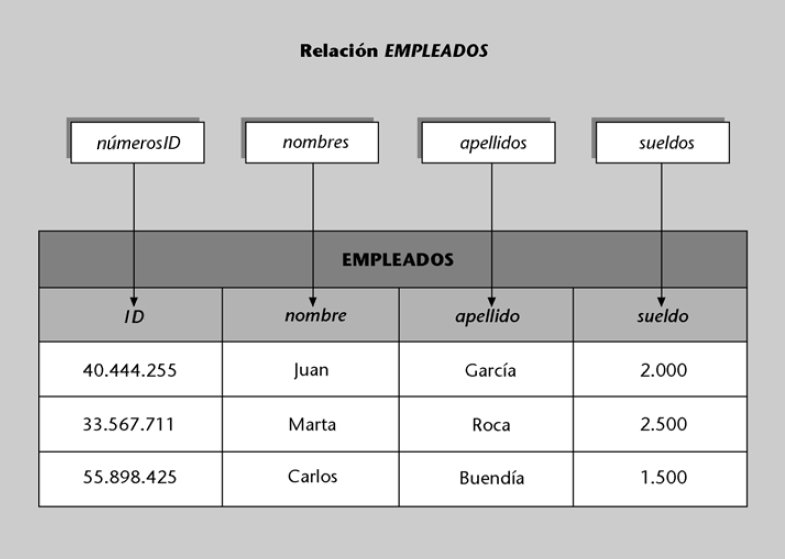
\includegraphics[width=8cm]{imagenes/01_tabla1.png}
\caption{Visualizaci�n de una relaci�n.}
\label{fig:tabla1}
\end{figure}

Luego de esta explicaci�n, se puede definir formalmente que son las \textit{relaciones}, adem�s de otros conceptos vinculados con ellas. \\

\subsection{Definici�n de Relaci�n}
\label{defrel}

Un \textbf{dominio $D$} es un conjunto de valores at�micos, es decir, indivisibles. �stos pueden ser de dos tipos: \textit{dominios predefinidos} que son los tipos de datos que proporcionan los lenguajes de bases de datos, por ejemplo los enteros, cadena de caracteres, reales, entre otros; y los \textit{dominios definidos por el usuario}, que pueden ser m�s espec�ficos. Estos �ltimos deben constar con un nombre de dominio y una descripci�n de valores que forman parte de �l, por ejemplo el dominio de edades de los trabajadores se denomina \textit{dom\_edad} y �ste contiene valores enteros entre 16 y 65 \cite{campus2006}. \\

Una \textbf{relaci�n $R$} consta de un \textit{esquema} y una \textit{extensi�n}. Como se muestra en la Figura \ref{fig:tabla2} \cite{campus2006}, el esquema es el nombre de la tabla junto con el nombre de sus columnas. El \textbf{esquema de la relaci�n} contiene el nombre de la relaci�n y un conjunto de atributos, es decir, $R({A}_{1},{A}_{2},...,{A}_{n})$, donde $R$ es el nombre de la relaci�n y ${A}_{1},{A}_{2},...,{A}_{n}$ es una lista de \textbf{atributos}. Cada \textbf{atributo $A_{i}$} es el nombre del rol que ejerce un \textit{dominio $D$} en un esquema de relaci�n, por ejemplo al revisar la Figura \ref{fig:tabla1}, se observa que el \textit{atributo} \textit{nombre} se refiere a los nombres de los empleados que ser�n almacenados en esa \textit{tabla}. \textit{$D$} es el \textbf{dominio de $A_{i}$} y se denota por $dom(A_{i})$ \cite{campus2006,elmasri2002fundamentos}. \\

\begin{figure}[h!]
\centering
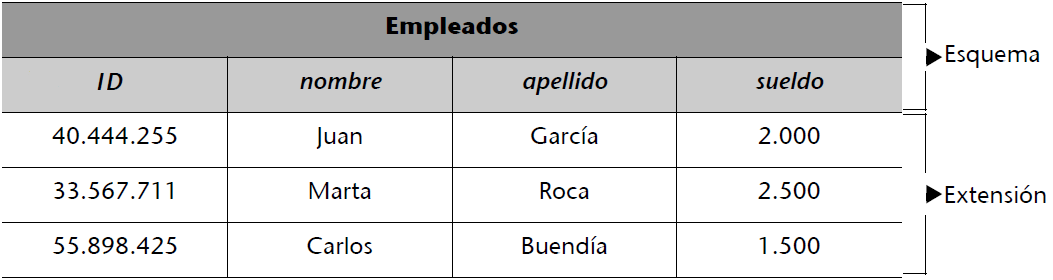
\includegraphics[width=10cm]{imagenes/02_tabla2.png}
\caption{Esquema y Extensi�n de una Relaci�n.}
\label{fig:tabla2}
\end{figure}

Cada \textit{atributo} es �nico, por ende no tiene sentido que un mismo \textit{dominio} realice dos veces el mismo rol en un mismo \textit{esquema}. Por ende, no existen dos \textit{atributos} con el mismo nombre en un \textit{esquema}, pero s� se puede repetir un nombre de un \textit{atributo} en distintas \textit{relaciones}. Por ejemplo, no tendr�a sentido que el \textit{atributo} \textit{nombre} de la \textit{tabla} que se presenta en la Figura \ref{fig:tabla2} se repita por cada \textit{tupla}, a menos que se desee guardar el segundo nombre de ellos, entonces ese nuevo \textit{atributo} estar�a realizando un rol distinto al anterior. Los \textit{dominios} no necesariamente deben ser diferentes en una \textit{relaci�n}\cite{campus2006}. \\

La \textbf{extensi�n de la relaci�n} del esquema $R({A}_{1},{A}_{2},...,{A}_{n})$ es un conjunto de \textbf{$n$-tuplas} $r=\lbrace t_{1},t_{2},...,t_{m} \rbrace$. Cada \textbf{$n$-tupla} es una lista de $n$ valores $t= <v_{1},v_{2},...,v_{n}>$, donde cada valor $v_{i}$ con $1 \leq i \leq n$, es un elemento de $dom(A_{i})$ o un valor especial denominado \textit{nulo}. Los valores \textit{nulos} representan los \textit{atributos} cuyos valores no existen para algunas \textit{tuplas} o simplemente se desconocen. Al denotar el esquema de la Figura \ref{fig:tabla1} como \emph{EMPLEADOS}$(ID,nombre,apellido,sueldo)$ el conjunto de \textbf{tuplas} se muestra en en la Figura \ref{fig:tabla3} \cite{campus2006,elmasri2002fundamentos}. \\

\begin{figure}[h!]
\centering
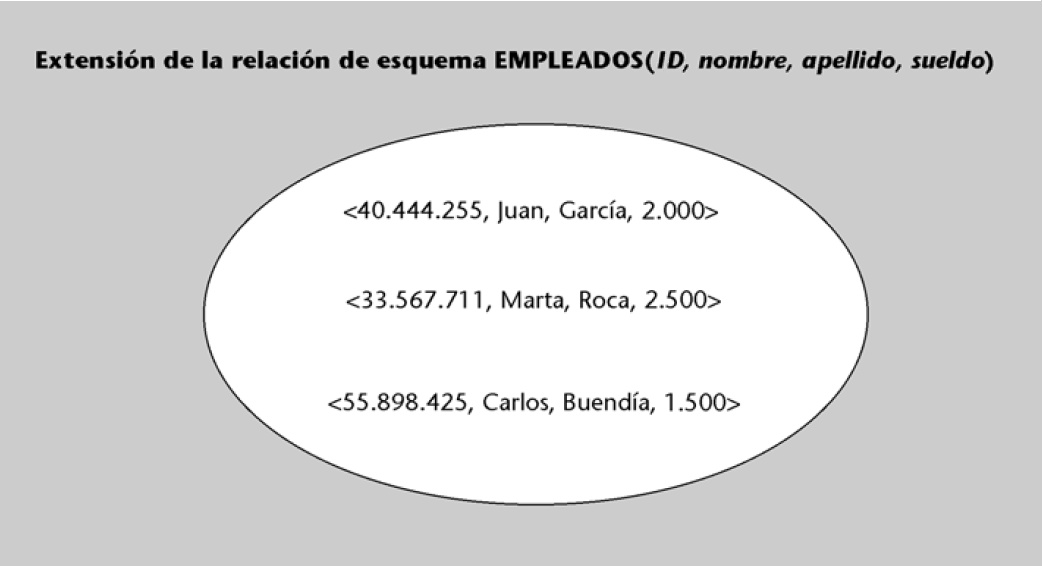
\includegraphics[width=10cm]{imagenes/03_tabla3.png}
\caption{Extensi�n de la relaci�n de un esquema.}
\label{fig:tabla3}
\end{figure}

El \textbf{grado} de una \textit{relaci�n} es el n�mero de \textit{atributos} que pertenecen a su \textit{esquema}. Por ejemplo, de la Figura \ref{fig:tabla3} se aprecia que el grado de la relaci�n del esquema es 4 \cite{campus2006}. \\

La \textbf{cardinalidad} de una \textit{relaci�n} es el n�mero de tuplas que pertenecen a su extensi�n. Por ejemplo, observando la Figura \ref{fig:tabla3} se intuye que la cardinalidad de la relaci�n es 3 \cite{campus2006}. \\

\subsection{Relaciones v/s Archivos}
\label{relvsfic}

A continuaci�n se explican las diferencias entre relaciones y archivos. A simple vista ambos resultan similares, pero a pesar de esto, el Modelo Relacional define ciertas caracter�sticas que hacen de los archivos cl�sicos totalmente diferentes de las relaciones. \\

\begin{enumerate}

\item \textbf{Atomicidad de los valores de los atributos}: como se explic� en la Secci�n \ref{defrel}, los valores de los \textit{atributos} de una \textit{relaci�n} no deben tener una estructura interna, ya que siempre deben tomar un valor de su \textit{dominio} o un valor \textit{nulo}. Se define \textit{nulo} como un valor que representa la informaci�n desconocida o que no se puede aplicar para ciertas \textit{tuplas} \cite{campus2006}. \\

\item \textbf{No-repetici�n de las tuplas}: en un archivo se puede dar el caso de que dos registros tengan los mismos datos. En el Modelo Relacional no es posible que una relaci�n tenga \textit{tuplas} repetidas. Tal como se dijo en la Secci�n \ref{defrel}, la \textit{extensi�n} es un conjunto de \textit{tuplas}, y en un conjunto no existen elementos repetidos \cite{campus2006}. \\

\item \textbf{No-ordenaci�n de las tuplas}: anteriormente en la Secci�n \ref{defrel} se especific� que la \textit{extensi�n} de una \textit{relaci�n} es un conjunto de \textit{tuplas}, por ende no es posible que haya ordenaci�n entre los elementos de un conjunto. La idea es conseguir que se puedan representar los datos en un nivel abstracto, independiente de su estructura en el mundo real. A pesar de que los SGBD almacenan las \textit{tuplas} en un orden en concreto dada su implementaci�n f�sica, esto no es visible si se trabaja a un nivel conceptual. De alguna forma, no tiene sentido consultar por "la primera tupla" en una relaci�n. �sto dista completamente de como se trabaja en un archivo, donde el orden s� es importante a la hora de manipular datos \cite{campus2006}.\\

\item \textbf{No-ordenaci�n de los atributos}: Un esquema $R$ consta de un conjunto de atributos  $\lbrace A_{1},A_{2},...,A_{n} \rbrace$, tal como se defini� en la Secci�n \ref{defrel}. As�, no hay orden entre los atributos ya que �stos tambi�n forman un conjunto. La idea es representar los hechos independientemente de su estructura real, a diferencia de los archivos donde la estructura de los datos al almacenarlos o manipularlos, deben seguir un orden pre-establecido \cite{campus2006}. \\

\end{enumerate}

\subsection{Claves en las Relaciones}
\label{clavesrel}

Toda informaci�n contenida en una Base de Datos se debe identificar de alguna manera. En el Modelo Relacional, se utilizan las llamadas  \textit{claves}. En esta secci�n se define qu� es una \textit{clave candidata, clave primaria y clave alternativa} en una relaci�n, pero antes se debe definir el concepto de \textit{superclave}. \\

Una \textbf{superclave} de una \textit{relaci�n de esquema} $R(A_{1},A_{2},...,A_{n})$ es un subconjunto de atributos tal que no puede haber dos \textit{tuplas} que tengan la misma combinaci�n de valores para los \textit{atributos} de ese subconjunto. �sto permite identificar y diferenciar todas las \textit{tuplas} que contiene una \textit{relaci�n}, cumpli�ndose la propiedad que indica que toda relaci�n no debe tener \textit{tuplas} repetidas \cite{campus2006}. \\

Toda relaci�n por lo menos tiene una \textit{superclave} que es formada por todos los atributos de su esquema, esto podr�a ocasionar que tenga \textit{atributos} repetidos, ser�a m�s �til tener una \textit{clave} que carezca de redundancia. Una \textit{superclave m�nima} es una \textit{superclave} a la cual no se puede quitarle atributos sin que deje de cumplirse la restricci�n de unicidad \cite{elmasri2002fundamentos}. \\

En general, un \textit{esquema de relaci�n} puede tener m�s de una clave y a cada una de ellas se le llama \textbf{clave candidata}. Es com�n definir a una de las \textit{claves candidatas} como \textbf{clave primaria} y sirven para identificar las \textit{tuplas} en una relaci�n, adem�s es posible que una \textit{clave primaria} conste de m�s de un \textit{atributo}. Las \textit{claves candidatas} que no sean elegidas como primaria se les llama \textbf{claves alternativas} \cite{elmasri2002fundamentos,campus2006}. \\

\subsection{Claves For�neas en las Relaciones}
\label{clavesext}

Hasta ahora se ha explicado las relaciones en forma individual, pero en una Base de Datos Relacional existen m�s de una relaci�n para explicar distintos tipos de hechos que ocurren en el mundo real, adem�s de los posibles lazos o v�nculos que �stos tengan. \\ 

De manera formal se define que una \textbf{clave for�neas} de una \textit{relaci�n} $R$ es un subconjunto de \textit{atributos} del \textit{esquema}, que denominamos \textit{CF} y debe cumplir las siguientes condiciones: \\

\begin{enumerate}

\item Existe una relaci�n $S$ ($S$ no debe ser necesariamente diferente de $R$) y que tiene por clave primar�a a \textit{CP} \cite{campus2006}. \\

\item Se cumple que, para toda tupla $t$ de la extensi�n de $R$, los valores para \textit{CF} son nulos o coinciden con los valores para \textit{CP} de alguna tupla $s$ de $S$ \cite{campus2006}.\\

\end{enumerate}

Entonces, se dice que la clave for�nea \textit{CF} referencia a la clave primaria \textit{CP} de la relaci�n $S$, y tambi�n que la clave for�nea \textit{CF} referencia a la relaci�n $S$ \cite{campus2006}. \\

En la Figura \ref{fig:tupla1} \cite{campus2006} se muestra un ejemplo de claves for�neas. La relaci�n $\emph{EMPLEADOS}$ tiene dos claves for�neas: una es el $\lbrace$\textit{IDjefe}$\rbrace$ que referencia la clave primaria de la misma relaci�n indicando que para cada empleado qui�n es su jefe y los atributos $\lbrace$\textit{edificiodesp, numerodesp}$\rbrace$ que se refieren a la clave primaria de la relaci�n despachos e indica el despacho donde trabaja cada empleado \cite{campus2006}. \\

\begin{figure}[h!]
\centering
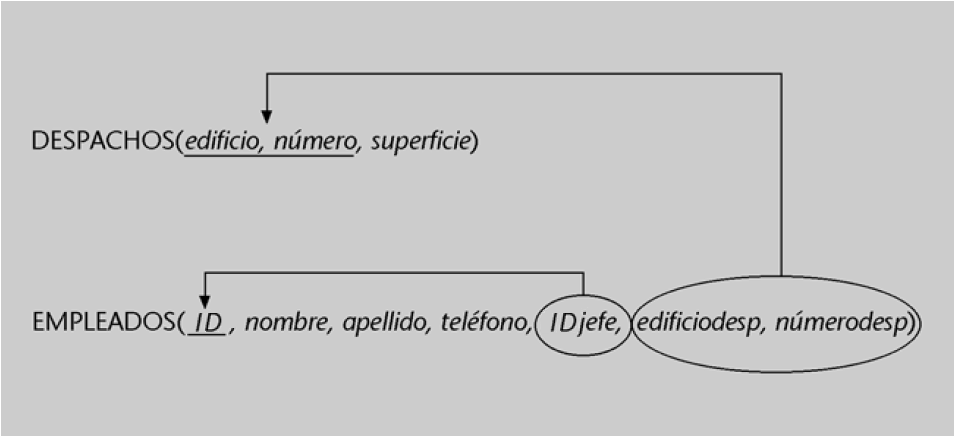
\includegraphics[width=10cm]{imagenes/04_tupla.png}
\caption{Ejemplo de clave for�nea.}
\label{fig:tupla1}
\end{figure}

Dada la definici�n de \textit{clave for�nea}, es posible extraer algunas consecuencias: \\

\begin{enumerate}

\item Si una clave for�nea \textit{CF} referencia a una clave primaria \textit{CP}, entonces la cantidad de atributos de \textit{CF} y de \textit{CP} deben coincidir. Como se muestra en la Figura \ref{fig:tupla1}, tanto la clave for�nea $\lbrace$\textit{edificiodeso, numerodesp}$\rbrace$ y la clave primaria $\lbrace$\textit{edificio, numero}$\rbrace$  tienen dos atributos \cite{campus2006}. \\

\item Dado lo anterior, se puede establecer una biyecci�n entre los atributos de la clave for�nea y los atributos de la clave primaria que referencia. De la Figura \ref{fig:tupla1}, \textit{edificiodesp} le corresponde a \textit{edificio}, y \textit{numerodesp} le corresponde a \textit{numero} \cite{campus2006}. \\ 

\item Los domino de los atributos de la clave for�nea deben coincidir con los dominios de los atributos de la clave primaria a la que referencia. Por ejemplo, de la Figura \ref{fig:tupla1} se aprecia que \textit{dom(edificioesp)} $=$ \textit{dom(edificio)} y \textit{dom(numerodesp)} $=$ \textit{dom(numero)} \cite{campus2006}. \\

\end{enumerate}

\subsection{Reglas de Integridad}
\label{reglasint}

Se denomina \textbf{integridad} a la \textit{``propiedad de los datos de representar posibles casos del mundo real''} \cite{campus2006}. Para hacer efectivo que los datos sean �ntegros, es preciso que se cumplan una serie de condiciones, �stas pueden ser de dos tipos: \\

\begin{enumerate}

\item Las \textbf{restricciones de integridad de usuario} que son definida por los mismos. Ellas se cumplen en bases de datos particulares, ya que posiblemente no son relevantes en otras. Por ejemplo, no pueden existir sueldos negativos \cite{campus2006}. \\

\item Las \textbf{reglas de integridad del modelo} son condiciones generales propias del Modelo Relacional, y �stas deben se deben cumplir en toda base de datos que est�n bajo este modelo \cite{campus2006}. \\

\end{enumerate}

A continuaci�n se describir�n las \textit{reglas de integridad de modelo} con un mayor detalle. Es importante agregar que todo SGBD que sea relacional, debe obligar y cumplir estas restricciones. \\

\subsubsection{Regla de Integridad de Unicidad de la Clave Primaria}

\textit{``La \textbf{regla de integridad de unicidad de la clave primaria} indica que si el conjunto de atributos de $CP$ es clave primaria de una relaci�n $R$, entonces la extensi�n de $R$ no puede tener dos tuplas con la misma combinaci�n de valores para los atributos de $CP$''} \cite{campus2006}. Es decir, toda clave primaria que se elija para una relaci�n no debe tener valores repetidos. \\

\subsubsection{Regla de Integridad de Entidad de la Clave Primaria}

\textit{``La \textbf{regla de integridad de entidad de la clave primaria} establece que si el conjunto de atributos $CP$ es la clave primaria de una relaci�n $R$, la extensi�n de $R$ no debe tener ninguna tupla con alg�n valor nulo para ninguno de los atributos de $CP$''} \cite{campus2006}. En otras palabras, los atributos de clave primara de alguna relaci�n no deben ser nulos, de esta manera, es posible identificar las tuplas de las relaciones. \\

\subsubsection{Regla de Integridad Referecial}

\textit{``La \textbf{regla de integridad referencial} indica que si un conjunto de atributos $CF$ es una clave for�nea de una relaci�n $R$ que referencia a una relaci�n $S$ no necesariamente diferente a $R$, que tiene por clave primaria $CP$, entonces, para toda tupla $t$ de la extensi�n $R$, los valores del conjunto de atributos $CF$ de $t$ son valores nulos o que coinciden con los valores para $CP$ de alguna tupla $s$ de $S$''} \cite{campus2006}. O sea, los valores de una clave for�nea deben ser nulos o deben existir en la clave primaria que referencian. \\

\subsubsection{Regla de Integridad de Dominio}

Dentro de esta regla, existen dos condiciones: \\

\begin{enumerate}

\item La \textbf{primera condici�n} consiste en que \textit{``un valor no nulo de un atributo $A_{i}$ debe pertenecer a $dom(A_{i})$''} \cite{campus2006}. �sto implica que todos los valores distintos de nulo que contengan la base de datos para cierto atributo debe pertenecer al dominio declarado de ese atributo. \\

\item La \textbf{segunda condici�n} sirve para \textit{``establecer que los operadores pueden aplicarse sobre los valores dependen de los valores, es decir, un operador determinado s�lo se puede aplicar sobre valores que tengan dominios que le sean adecuados''} \cite{campus2006}. \\

\end{enumerate}

\subsection{Operaciones de Actualizaci�n}
\label{operactua}

En el Modelo Relacional, es posible clasificar las operaciones en 2 tipos: \textit{recuperaciones} y \textit{actualizaciones}. Las operaciones de recuperaci�n ser�n atendidas en la Secci�n \ref{algebrarel}, en esta secci�n se presentan las operaciones b�sicas de actualizaci�n. \\

\textit{\textbf{La actualizaci�n} de los datos consiste en realizar que los cambios que suceden en la realidad se reflejen en la base de datos} \cite{campus2006}. Existen tres operadores b�sicos de actualizaci�n, cada uno de ellas deben seguir las \textit{reglas de integridad} que fueron explicadas en la Secci�n \ref{reglasint}: \\

\begin{itemize}

\item \textbf{Inserci�n}: sirve para a�adir una o m�s tuplas a una relaci�n. La inserci�n puede violar cualquiera de los cuatro tipos de restricciones. Por ejemplo, las restricciones de dominio se violan si se da un valor de atributo que no aparezca en el dominio que le corresponde, las restricciones de clave son violadas si un valor clave de la tupla ya existe en dicha relaci�n, la integridad de entidades se violan si la clave primaria de la nueva tupla es nula y la integridad referencial es transgredida si el valor de cualquier clave for�nea hace referencia a una tupla que no existe en la relaci�n referenciada \cite{elmasri2002fundamentos,campus2006}.  \\

\item \textbf{Eliminaci�n}: que sirve para eliminar una o m�s tuplas de una relaci�n. Esta operaci�n s�lo puede violar la integridad referencial si las claves for�neas de otras tuplas hacen referencia a la tupla que se desea eliminar \cite{elmasri2002fundamentos,campus2006}. \\

\item \textbf{Actualizaci�n}: o modificaci�n, sirve para cambiar los valores de una o m�s tuplas en una relaci�n para uno o m�s de sus atributos. Modificar un valor es equivalente a eliminar una tupla e insertar una nueva con los datos modificados, por ende, las restricciones violadas tanto para la \textit{inserci�n} como la \textit{eliminaci�n} pueden ser transgredidas en esta operaci�n \cite{elmasri2002fundamentos,campus2006}. \\

\end{itemize}

\section{�lgebra Relacional}
\label{algebrarel}

En la Secci�n \ref{operactua} se han explicado las operaciones de actualizaci�n en una base de datos relacional. En la presente secci�n se ahondar� a fondo en las operaciones de recuperaciones o manipulaciones de los datos, el \textbf{�lgebra Relacional}. \\

El \textbf{�lgebra Relacional} contiene operaciones que permiten al usuario especificar peticiones de recuperaciones b�sicas. El resultado de estas operaciones es una nueva \textit{relaci�n} formada a partir de una o m�s \textit{relaciones}. Por ende, estas operaciones producen nuevas \textit{relaciones} que podr�n ser utilizadas para manipularse en un futuro utilizando operaciones de la misma �lgebra. A esta propiedad se le denomina \textbf{cierre relacional} \cite{elmasri2002fundamentos,campus2006}. \\

Dentro de las operaciones del \textit{�lgebra Relacional} existen dos grupos reconocidos: \\

\begin{enumerate}

\item \textbf{Operaciones espec�ficamente relacionales}: este grupo consiste en operaciones creadas espec�ficamente para las bases de datos relacionales \cite{elmasri2002fundamentos}. \\

\item \textbf{Operaciones conjuntistas}: �sta contiene el conjunto de operaciones de la teor�a matem�tica de conjuntos y es posible aplicarlas dado que las relaciones se definen como conjuntos de tuplas \cite{elmasri2002fundamentos}. \\

\end{enumerate}

En las siguientes secciones, se explicar�n cada una de las operaciones que respectan al �lgebra Relacional. En primera instancia se explicar� las operaciones \textit{seleccionar} y \textit{proyectar} ya que son las m�s sencillas de entender\cite{elmasri2002fundamentos}, luego se explicar�n las operaciones de conjuntos, finalizando con la \textit{reuni�n} y otro tipo de operaciones un poco m�s complejas \cite{elmasri2002fundamentos}. \\

Para un mayor entendimiento del lector, se presenta un ejemplo para ilustrar las operaciones del \textit{�lgebra Relacional} \cite{campus2006}, el cual ser� ampliamente utilizado en las secciones posteriores. \\

\begin{enumerate}

\item La relaci�n $\emph{EDIFICIOS\_EMP}$ contiene los distintos edificios de una empresa para desarrollar sus actividades. \\

\item La relaci�n $\emph{DESPACHOS}$ contiene los datos de los despachos de cada uno de los edificios anteriores. \\

\item La relaci�n $\emph{EMPLEADOS\_ADM}$ contiene los datos de los empleados de la empresa que llevan a cabo tareas administrativas. \\

\item La relaci�n $\emph{EMPLEADOS\_PROD}$ almacena los datos de los empleados de la empresa que se ocupan de las tarea de producci�n. \\

\end{enumerate}

La descripci�n y esquema de las relaciones anteriores se muestran en las Tablas \ref{tab:01}, \ref{tab:02}, \ref{tab:03} y \ref{tab:04}. \\

%\begin{figure}[h!]
%\centering
%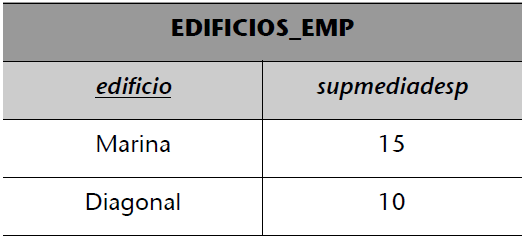
\includegraphics[width=4cm]{imagenes/05_edificioemp.png}
%\caption{Esquema y extensi�n de $EDIFICIOS\_EMP$.}
%\label{fig:edificioemp}
%\end{figure}

\clearpage
\begin{table}[h!]
\footnotesize
\centering
\begin{tabular}{|c|c|}
\hline
\multicolumn{2}{|c|}{\textbf{EDIFICIOS\_EMP}} \\ \hline
\textit{\underline{edificio}}   & \textit{supmediadesp}   \\ \hline
Marina              & 15                      \\ \hline
Diagonal            & 10                      \\ \hline
\end{tabular}
\caption{Esquema y extensi�n de \textit{EDIFICIOS\_EMP}.}
\label{tab:01}
\end{table}

%\begin{figure}[h!]
%\centering
%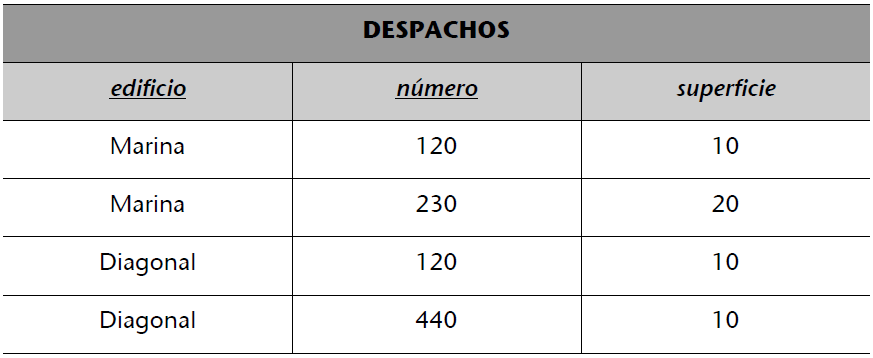
\includegraphics[width=7.5cm]{imagenes/06_despachos.png}
%\caption{Esquema y extensi�n de $DESPACHOS$.}
%\label{fig:despachos}
%\end{figure}

\begin{table}[h!]
\footnotesize
\centering
\begin{tabular}{|c|c|c|}
\hline
\multicolumn{3}{|c|}{\textbf{DESPACHOS}}                  \\ \hline
\textit{\underline{edificio}} & \textit{\underline{numero}} & \textit{superficie} \\ \hline
Marina            & 120             & 10                  \\ \hline
Marina            & 230             & 20                  \\ \hline
Diagonal          & 120             & 10                  \\ \hline
Diagonal          & 440             & 10                  \\ \hline
\end{tabular}
\caption{Esquema y extensi�n de \textit{DESPACHOS}.}
\label{tab:02}
\end{table}

%\begin{figure}[h!]
%\centering
%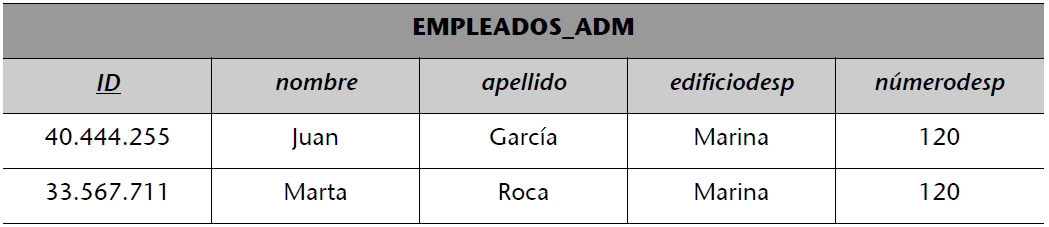
\includegraphics[width=8.5cm]{imagenes/07_empleadosadm.png}
%\caption{Esquema y extensi�n de $EMPLEADOS\_ADM$.}
%\label{fig:empleadosadm}
%\end{figure}

\begin{table}[h!]
\footnotesize
\centering
\begin{tabular}{|c|c|c|c|c|}
\hline
\multicolumn{5}{|c|}{\textbf{EMPLEADOS\_ADM}}                                                    \\ \hline
\textit{\underline{ID}} & \textit{nombre} & \textit{apellido} & \textit{edificiodesp} & \textit{numerodesp} \\ \hline
40.444.255   & Juan            & Garc�a            & Marina                & 120                 \\ \hline
33.567.711   & Marta           & Roca              & Marina                & 120                 \\ \hline
\end{tabular}
\caption{Esquema y extensi�n de \textit{EMPLEADOS\_ADM}.}
\label{tab:03}
\end{table}

%\begin{figure}[h!]
%\centering
%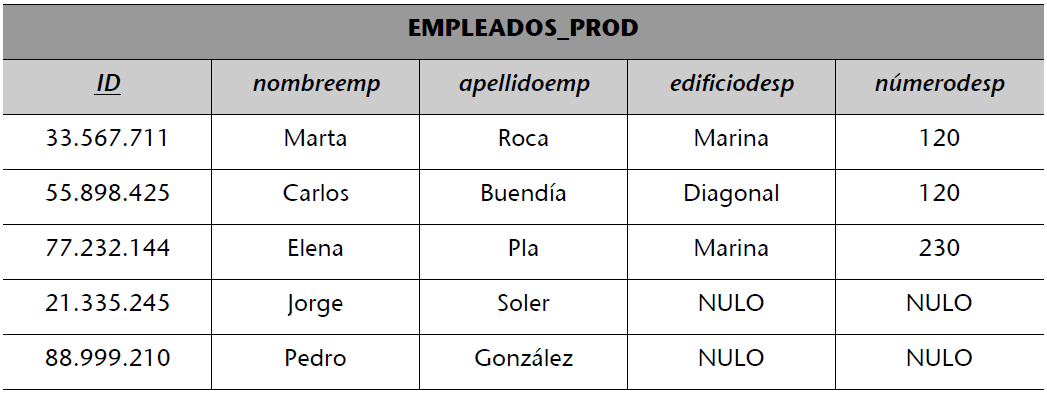
\includegraphics[width=9cm]{imagenes/08_empleadosprod.png}
%\caption{Esquema y extensi�n de $EMPLEADOS\_PROD$.}
%\label{fig:empleadosprod}
%\end{figure}

\begin{table}[h!]
\footnotesize
\centering
\begin{tabular}{|c|c|c|c|c|}
\hline
\multicolumn{5}{|c|}{\textbf{EMPLEADOS\_PROD}}                                                         \\ \hline
\textit{\underline{ID}} & \textit{nombreemp} & \textit{apellidoemp} & \textit{edificiodesp} & \textit{numerodesp} \\ \hline
33.567.711   & Marta              & Roca                 & Marina                & 120                 \\ \hline
55.898.425   & Carlos             & Buend�a              & Diagonal              & 120                 \\ \hline
77.232.144   & Elena              & Pla                  & Marina                & 230                 \\ \hline
21.335.245   & Jorge              & Soler                & NULO                  & NULO                \\ \hline
88.999.210   & Pedro              & Ginz�lez             & NULO                  & NULO                \\ \hline
\end{tabular}
\caption{Esquema y extensi�n de \textit{EMPLEADOS\_PROD}.}
\label{tab:04}
\end{table}

\subsection{Selecci�n}
\label{selec}

La operaci�n \textbf{selecci�n} sirve para seleccionar un subconjunto de tuplas de una relaci�n que satisfacen alguna \textbf{condici�n de selecci�n}. Se denota la operaci�n \textbf{selecci�n} como se muestra en la Consulta \ref{eq:01} \\

\begin{equation}
\sigma_{<condicion\_de\_seleccion>}(R)
\label{eq:01}
\end{equation}
\\

donde $\sigma$ es el operador de \textbf{selecci�n} y la condici�n de selecci�n es una expresi�n booleana que se especifica en t�rminos de los atributos de la relaci�n $R$. El resultado de esta operaci�n tiene los mismos atributos que $R$. La expresi�n booleana se descompone de una o m�s cl�usulas, como se muestra en la Consulta \ref{eq:02} � \ref{eq:03}. \\

\begin{equation}
<nombre\_de\_atributo> <operador\_de\_comparacion> <valor\_constante>
\label{eq:02}
\end{equation}
\\
\begin{equation}
<nombre\_de\_atributo> <operador\_de\_comparacion> <nombre\_de\_atributo>
\label{eq:03}
\end{equation}
\\

donde $nombre\_de\_atributo$ es el nombre de alg�n atributo de $R$, $operador\_de\_comparacion$ es uno de los operadores $\lbrace =, <, \leq, >, \geq, \neq \rbrace$, y $valor\_constante$ es un valor perteneciente al dominio del atributo. Las cl�usulas pueden conectarse mediante los operadores booleanos AND ($\wedge$), OR ($\vee$), y NOT ($�$), formando una condici�n m�s general \cite{elmasri2002fundamentos}. \\

El operador \textit{selecci�n} s�lo se aplica a una relaci�n. A su vez, esta operaci�n se aplica a cada tupla individualmente, por ende las condiciones de selecci�n no pueden implicar a m�s de una tupla. El \textbf{grado} del resultado de esta operaci�n es el mismo que $R$. El n�mero de tuplas resultante siempre es menor o igual al n�mero de tuplas de $R$ para cualquier condici�n. \cite{elmasri2002fundamentos}. \\

La operaci�n \textbf{seleccionar} es conmutativa, por ende se cumple la F�rmula \ref{eq:04}. \\

\begin{equation}
\sigma_{<cond1>}(\sigma_{<cond2>}(R)) = \sigma_{<cond2>}(\sigma_{<cond1>}(R))
\label{eq:04}
\end{equation}
\\

Adem�s, siempre se puede combinar una serie de operaciones \textbf{selecci�n} en una sola operaci�n con una condici�n conjuntiva ($\wedge$), como se muestra en la F�rmula \ref{eq:05}. \\

\begin{equation}
\sigma_{<cond1>}(\sigma_{<cond2>}(...(\sigma_{<condn>}(R))...)) = \sigma_{<cond1> \wedge <cond2> \wedge ... \wedge <condn>}(R)
\label{eq:05}
\end{equation}
\\

Por ejemplo, si se desea obtener una relaci�n $R$ con los despachos en el edificio Marina y que tienen una superficie de m�s de 12 metros cuadrados, la operaci�n queda como se muestra en la Consulta \ref{eq:06}. \\

\begin{equation}
\sigma_{edificio = Marina \wedge superficie > 12}(\emph{DESPACHOS})
\label{eq:06}
\end{equation}
\\

El resultado gr�fico de la Consulta \ref{eq:06} se aprecia en la Tabla \ref{tab:ejemplo1}. \\

%\begin{figure}[h!]
%\centering
%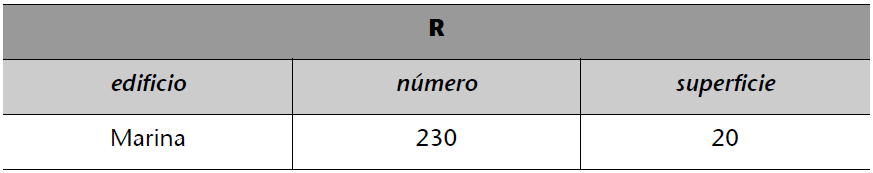
\includegraphics[width=9cm]{imagenes/09_ejemplo1.png}
%\caption{Restultado gr�fico de una selecci�n}
%\label{fig:ejemplo1}
%\end{figure}

\begin{table}[h!]
\footnotesize
\centering
\begin{tabular}{|c|c|c|}
\hline
\multicolumn{3}{|c|}{\textbf{R}}                          \\ \hline
\textit{edificio} & \textit{numero} & \textit{superficie} \\ \hline
Marina            & 230             & 20                  \\ \hline
\end{tabular}
\caption{Restultado gr�fico de una selecci�n}
\label{tab:ejemplo1}
\end{table}

\subsection{Proyecci�n}
\label{selec}

Si se desea extraer ciertos atributos de una relaci�n, entonces se usa la operaci�n \textbf{proyecci�n} para seleccionar esos atributos y desechar los otros. Esta operaci�n se muestra en la Consulta \ref{eq:07}. \\

\begin{equation}
\pi_{<lista\_de\_atributos>}(R)
\label{eq:07}
\end{equation}
\\

donde $\pi$ es el s�mbolo utilizado para representar la \textbf{proyecci�n} y $lista\_de\_atributos$ es una lista de atributos de la relaci�n $R$. El resultado de la \textbf{proyecci�n} contiene �nicamente los atributos especificados y en el mismo orden que se especifican. Su grado es igual al n�mero de atributos en $lista\_de\_atributos$. Adem�s, esta operaci�n elimina cualquier tupla repetida. A esto se le conoce como \textbf{eliminaci�n de duplicados} \cite{elmasri2002fundamentos}. \\

El n�mero de tuplas de la relaci�n resultante de la operaci�n \textbf{proyecci�n} es menor o igual que el numero de tuplas de $R$. Si la lista de atributos a proyectar es una superclave de $R$, entonces el resultado tendr� el mismo n�mero de tuplas que $R$ \cite{elmasri2002fundamentos}. Adem�s se cumple lo que se muestra en la Consulta \ref{eq:08}

\begin{equation}
\pi_{<lista1>}(\pi_{<lista2>}(R)) = \pi_{<lista1>}(R)
\label{eq:08}
\end{equation}
\\

�sto, siempre que $lista1$ sea un subconjunto de los atributos de $lista2$, sino el lado izquierdo ser� incorrecto. A su vez, la \textbf{proyecci�n} no es una operaci�n conmutativa \cite{elmasri2002fundamentos}. \\

Por ejemplo, se desea obtener una relaci�n $R$ con el nombre y apellido de todos los empleados de la relaci�n $\emph{EMPLEADOS\_ADM}$, entonces la operaci�n se hace como se muestra en la Consulta \ref{eq:09}. \\

\begin{equation}
\pi_{nombre,apellido}(\emph{EMPLEADOS\_ADM})
\label{eq:09}
\end{equation}
\\

El resultado gr�fico de la Consulta \ref{eq:09} se muestra en la Tabla \ref{tab:ejemplo2} \\.

%\begin{figure}[h!]
%\centering
%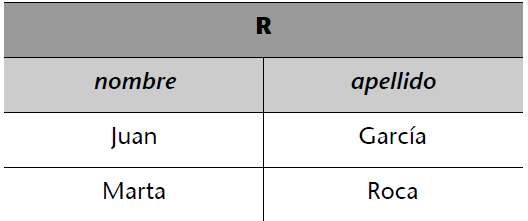
\includegraphics[width=6cm]{imagenes/10_ejemplo2.png}
%\caption{Restultado gr�fico de una proyecci�n}
%\label{fig:ejemplo2}
%\end{figure}

\begin{table}[h!]
\footnotesize
\centering
\begin{tabular}{|c|c|}
\hline
\multicolumn{2}{|c|}{\textbf{R}}    \\ \hline
\textit{nombre} & \textit{apellidp} \\ \hline
Juan            & Garc�a            \\ \hline
Marta           & Roca              \\ \hline
\end{tabular}
\caption{Restultado gr�fico de una proyecci�n.}
\label{tab:ejemplo2}
\end{table}

\subsection{Renombrar y Asignaci�n de Relaciones}
\label{renomb}

Es posible que se necesite aplicar varias operaciones de \textit{�lgebra Relacional}. Para esto, se puede escribir las operaciones en una sola expresi�n de \textit{�lgebra Relacional} anid�ndolas, o se puede aplicar una operaci�n a la vez y crear relaciones con resultados intermedios, renombrando estos �ltimos \cite{elmasri2002fundamentos}. La operaci�n \textbf{renombrar} cuando se aplica a una relaci�n $R$ de grado $n$ se denota como se muestra en la Consulta \ref{eq:10} � \ref{eq:11} � \ref{eq:12}. \\

\begin{equation}
\rho_{S(B_{1}, B_{2}, ..., B_{n})}(R)
\label{eq:10}
\end{equation}
\\
\begin{equation}
\rho_{S}(R)
\label{eq:11}
\end{equation}
\\
\begin{equation}
\rho_{(B_{1}, B_{2}, ..., B_{n)}}(R)
\label{eq:12}
\end{equation}
\\

El s�mbolo $\rho$ se refiere a la operaci�n \textbf{renombrar}, $S$ es el nuevo nombre de la relaci�n, y $B_{1}, B_{2}, ..., B_{n}$ son los nuevos nombres de los atributos. La primera expresi�n renombra la relaci�n y los atributos, la segunda renombre solamente la relaci�n y la tercera �nicamente los atributos. Si los atributos de $R$ son $(A_{1}, A_{2}, ..., A_{n})$ en ese orden, entonces cada $A_{i}$ se renombra como $B_{i}$ \cite{elmasri2002fundamentos}. \\

En algunos casos, resulta c�modo \textbf{asignar} relaciones resultantes de alguna consulta cuando se desea hacer muchas operaciones anidadas. Para esto se utiliza la operaci�n \textbf{asignar}, como se denota en la Consulta \ref{eq:14}. \\

%Para mayor comodidad y para evitar el excesivo uso de par�ntesis, la operaci�n \textbf{renombrar} se denota como se muestra en la consulta \ref{eq:13} � \ref{eq:14} � \ref{eq:15}. \\

%\begin{equation}
%S(B_{1}, B_{2}, ..., B_{n}) \leftarrow R
%\label{eq:13}
%\end{equation}
%\\
\begin{equation}
S \leftarrow R
\label{eq:14}
\end{equation}
\\
%\begin{equation}
%B_{1}, B_{2}, ..., B_{n}) \leftarrow R
%\label{eq:15}
%\end{equation}
%\\

Donde $\leftarrow$ indica la acci�n \textbf{renombrar}, $S$ el nuevo nombre de la relaci�n y $R$ la relaci�n antes de ser renombrada. \\

Por ejemplo, si se desea obtener una relaci�n $R$ con los despachos que est�n en el edificio Marina y tienen una superficie de m�s de 12 metros cuadrados, y adem�s extraer �nicamente el n�mero de ese departamento, la operaci�n se formula como se muestra en la Consulta \ref{eq:16} y \ref{eq:17}. \\

\begin{equation}
AUX \leftarrow \sigma_{edificio = Marina \wedge superficie > 12}(\emph{DESPACHOS})
\label{eq:16}
\end{equation}
\\
\begin{equation}
\pi_{numero}(AUX)
\label{eq:17}
\end{equation}
\\

El resultado gr�fico de la Consulta \ref{eq:16} y la Consulta \ref{eq:17} se aprecia en la Tabla \ref{tab:ejemplo3}. Notar que se utiliz� la operaci�n \textbf{asignar} para generar una relaci�n intermedia en la Consulta \ref{eq:16} y utilizarla en la Consulta \ref{eq:17} \\.

%\begin{figure}[h!]
%\centering
%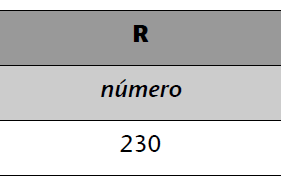
\includegraphics[width=3cm]{imagenes/11_ejemplo3.png}
%\caption{Restultado gr�fico de una selecci�n y una proyecci�n anidadas}
%\label{fig:ejemplo3}
%\end{figure}

\begin{table}[h]
\footnotesize
\centering
\begin{tabular}{|c|}
\hline
\textbf{R}      \\ \hline
\textit{numero} \\ \hline
230             \\ \hline
\end{tabular}
\caption{Resultado gr�fico de una selecci�n y una proyecci�n anidadas.}
\label{tab:ejemplo3}
\end{table}

\subsection{Operaciones de la Teor�a de Conjuntos}
\label{opteoriaconj}

En el Modelo Relacional, se utilizan varias operaciones de la \textbf{teor�a de conjuntos} para combinar de diversas maneras los elementos de dos conjuntos, entre ellas: \textbf{uni�n, intersecci�n y diferencia}. Estas tres operaciones son binaria, o sea, se aplican a dos conjuntos; y las relaciones implicadas deben tener el mismo tipo de tuplas. A esta �ltima condici�n se le llama \textbf{compatibilidad con la uni�n} \cite{elmasri2002fundamentos}. \\

De manera general, se dice que dos relaciones $R(A_{1}, A_{2}, ..., A_{n})$ y $S(B_{1}, B_{2}, ..., B_{n})$ son \textbf{compatibles con la uni�n} si tienen grado $n$ y si $dom(A_{i}) = dom(B_{i})$ para $1 \leq i \leq n$. Esto indica que las dos relaciones deben tener el mismo n�mero de atributos y que cada par de ellos tiene el mismo dominio \cite{elmasri2002fundamentos}. \\

\begin{itemize}

\item Se define la \textbf{uni�n} como una operaci�n cuyo resultado incluye todas las tuplas que est�n en $R$, en $S$ o en ambas. Adem�s, es importante recalcar que las tuplas resultantes que se repitan ser�n eliminadas. Esta operaci�n se denota como se muestra en la Consulta \ref{eq:18}. \\

\begin{equation}
R \cup S
\label{eq:18}
\end{equation}
\\

\item Se define la \textbf{intersecci�n} como una operaci�n cuyo resultado incluye todas las tuplas que est�n tanto en $R$ como en $S$, y es denotado como se muestra en la Consulta \ref{eq:19}. \\

\begin{equation}
R \cap S
\label{eq:19}
\end{equation}
\\

\item Se define \textbf{diferencia de conjuntos} como una operaci�n cuyo resultado es una relaci�n que incluye todas las tuplas que est�n en $R$ pero no en $S$, y se denota como se muestra en la Consulta \ref{eq:20}. \\

\begin{equation}
R - S
\label{eq:20}
\end{equation}
\\

\end{itemize}

Tanto la \textbf{uni�n} como la \textbf{intersecci�n} son operaciones conmutativas, por lo tanto se cumple la propiedad descrita por las Ecuaciones \ref{eq:21} y \ref{eq:22}. \\

\begin{equation}
R \cup S = S \cup R
\label{eq:21}
\end{equation}
\\
\begin{equation}
R \cap S = S \cap R
\label{eq:22}
\end{equation}
\\

Adem�s, la \textbf{uni�n} y la \textbf{intersecci�n} pueden tratarse como operaciones n-arias, y estas dos operaciones son asociativas, por lo tanto se cumple la propiedad descrita por las Ecuaciones \ref{eq:23} y \ref{eq:24}. \\

\begin{equation}
R \cup (S \cup T) = (R \cup S) \cup T
\label{eq:23}
\end{equation}
\\
\begin{equation}
R \cap (S \cap T) = (R \cap S) \cap T
\label{eq:24}
\end{equation}
\\

La operaci�n \textbf{diferencia} no es conmutativa, por lo tanto se cumple la propiedad descrita por la Ecuaci�n \ref{eq:25}. \\

\begin{equation}
R - S \neq S - R
\label{eq:25}
\end{equation}
\\

Por ejemplo, si necesita obtener una relaci�n $R$ que tenga a todos los empleados de la empresa, entonces utilizamos la \textbf{uni�n} de las relaciones \textit{EMPLEADOS\_ADM} y \textit{EMPLEADOS\_PROD} como se muestra en la Consulta \ref{eq:26}. \\

\begin{equation}
\emph{EMPLEADOS\_ADM} \cup \emph{EMPLEADOS\_PROD}
\label{eq:26}
\end{equation}
\\

El resultado gr�fico de la Consulta \ref{eq:26} se muestra en la Tabla \ref{tab:ejemplo4}.

%\begin{figure}[h!]
%\centering
%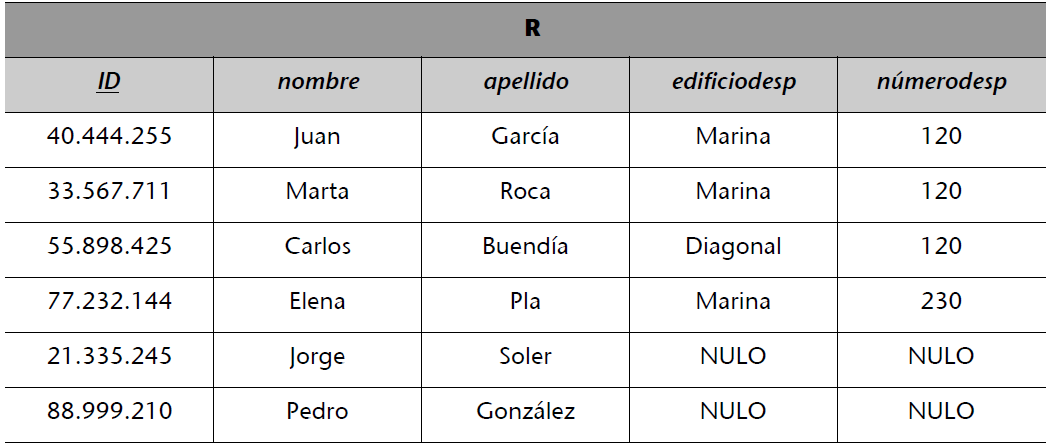
\includegraphics[width=10cm]{imagenes/12_ejemplo4.png}
%\caption{Restultado gr�fico de una uni�n}
%\label{fig:ejemplo4}
%\end{figure}

\begin{table}[h!]
\footnotesize
\centering
\begin{tabular}{|c|c|c|c|c|}
\hline
\multicolumn{5}{|c|}{\textbf{R}}                                                                 \\ \hline
\textit{\underline{ID}} & \textit{nombre} & \textit{apellido} & \textit{edificiodesp} & \textit{numerodesp} \\ \hline
40.444.255   & Juan            & Garc�a            & Marina                & 120                 \\ \hline
33.567.711   & Marta           & Roca              & Marina                & 120                 \\ \hline
55.898.425   & Carlos          & Buend�a           & Diagonal              & 120                 \\ \hline
77.232.144   & Elena           & Pla               & Marina                & 230                 \\ \hline
21.355.245   & Jorge           & Soler             & NULO                  & NULO                \\ \hline
88.999.210   & Pedro           & Gonz�lez          & NULO                  & NULO                \\ \hline
\end{tabular}
\caption{Resultado gr�fico de una uni�n.}
\label{tab:ejemplo4}
\end{table}

Si se necesita obtener una relaci�n $R$ que tenga a todos los empleados de la empresa que trabajen tanto en administraci�n como en producci�n, entonces se realiza una \textbf{intersecci�n} de las relaciones $\emph{EMPLEADOS\_ADM}$ y $\emph{EMPLEADOS\_PROD}$ como se muestra en la Consulta \ref{eq:27}. \\

\begin{equation}
\emph{EMPLEADOS\_ADM} \cap \emph{EMPLEADOS\_PROD}
\label{eq:27}
\end{equation}
\\

El resultado gr�fico de la Consulta \ref{eq:27} se muestra en la Tabla \ref{tab:ejemplo5}.

%\begin{figure}[h!]
%\centering
%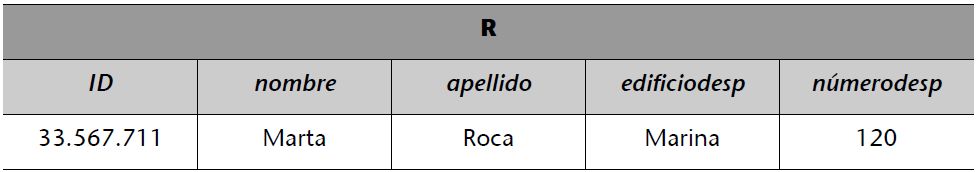
\includegraphics[width=10cm]{imagenes/13_ejemplo5.png}
%\caption{Restultado gr�fico de una intersecci�n}
%\label{fig:ejemplo5}
%\end{figure}

\begin{table}[h!]
\footnotesize
\centering
\begin{tabular}{|c|c|c|c|c|}
\hline
\multicolumn{5}{|c|}{\textbf{R}}                                                                 \\ \hline
\textit{ID} & \textit{nombre} & \textit{apellido} & \textit{edificiodesp} & \textit{numerodesp} \\ \hline
33.597.711   & Marta           & Roca              & Marina                & 120                 \\ \hline
\end{tabular}
\caption{Resultado gr�fico de una intersecci�n.}
\label{tab:ejemplo5}
\end{table}

Si se quiere obtener una relaci�n $R$ con todos los empleados de la empresa que trabajan en administraci�n, pero no en producci�n, se hace una \textbf{diferencia} entre las relaciones $\emph{EMPLEADOS\_ADM}$ y $\emph{EMPLEADOS\_PROD}$ como se muestra en la Consulta \ref{eq:28}. \\

\begin{equation}
\emph{EMPLEADOS\_ADM} \- \emph{EMPLEADOS\_PROD}
\label{eq:28}
\end{equation}
\\

El resultado gr�fico de la Consulta \ref{eq:25} se muestra en la Tabla \ref{tab:ejemplo6}.

%\begin{figure}[h!]
%\centering
%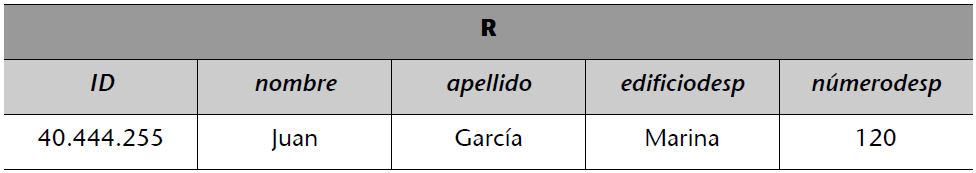
\includegraphics[width=10cm]{imagenes/14_ejemplo6.png}
%\caption{Restultado gr�fico de una diferencia}
%\label{fig:ejemplo6}
%\end{figure}

\begin{table}[h!]
\footnotesize
\centering
\begin{tabular}{|c|c|c|c|c|}
\hline
\multicolumn{5}{|c|}{\textbf{R}}                                                                 \\ \hline
\textit{ID} & \textit{nombre} & \textit{apellido} & \textit{edificiodesp} & \textit{numerodesp} \\ \hline
40.444.255   & Juan            & Garc�a            & Marina                & 120                 \\ \hline
\end{tabular}
\caption{Resultado gr�fico de una diferencia.}
\label{tab:ejemplo6}
\end{table}

A continuaci�n se explica la operaci�n \textbf{producto cartesiano}. �sta es una operaci�n binaria de conjuntos, pero las relaciones implicadas no necesariamente deben ser compatibles con la uni�n \cite{elmasri2002fundamentos}. \\

Se define \textbf{producto cartesiano} como una operaci�n que sirve para combinar tuplas de dos relaciones de forma combinatorial y se denota como se muestra en la Consulta \ref{eq:29}. \\

\begin{equation}
R \times S
\label{eq:29}
\end{equation}
\\

En general, el resultado de $R(A_{1}, A_{2}, ..., A_{n}) \times S(B_{1}, B_{2}, ..., B_{m})$ es una relaci�n $Q$ con $n + m$ atributos $Q(A_{1}, A_{2}, ..., A_{n}, B_{1}, B_{2}, ..., B_{m})$ en ese orden. $Q$ tiene una tupla por cada combinaci�n de tuplas entre $R$ y $S$. Por ende, si $R$ tiene $n_{r}$ tuplas y $S$ tiene $n_{s}$ tuplas, $R \times S$ tendr� $n_{r} \cdot n_{s}$ tuplas \cite{elmasri2002fundamentos}. \\

Por ejemplo, el \textbf{producto cartesiano} entre las relaciones $\emph{DESPACHOS}$ y $\emph{EDIFICOS\_EMP}$ se escribe como se muestra en la Consulta \ref{eq:30}. \\

\begin{equation}
\rho_{nombreedificio,supmediadesp}\emph{EDIFICIOS\_EMP} \times \emph{DESPACHOS}
\label{eq:30}
\end{equation}
\\

El resultado gr�fico de la Consulta \ref{eq:30} se aprecia en la Tabla \ref{tab:ejemplo7}. Para realizar esta operaci�n, fue necesario cambiar el nombre del atributo $edificio$ de la relaci�n $\emph{EDIFICOS\_EMP}$ por $nombreedificio$, para que no haya problema con el atributo $edificio$ de la relaci�n $\emph{DESPACHO}S$. \\

%\begin{figure}[h!]
%\centering
%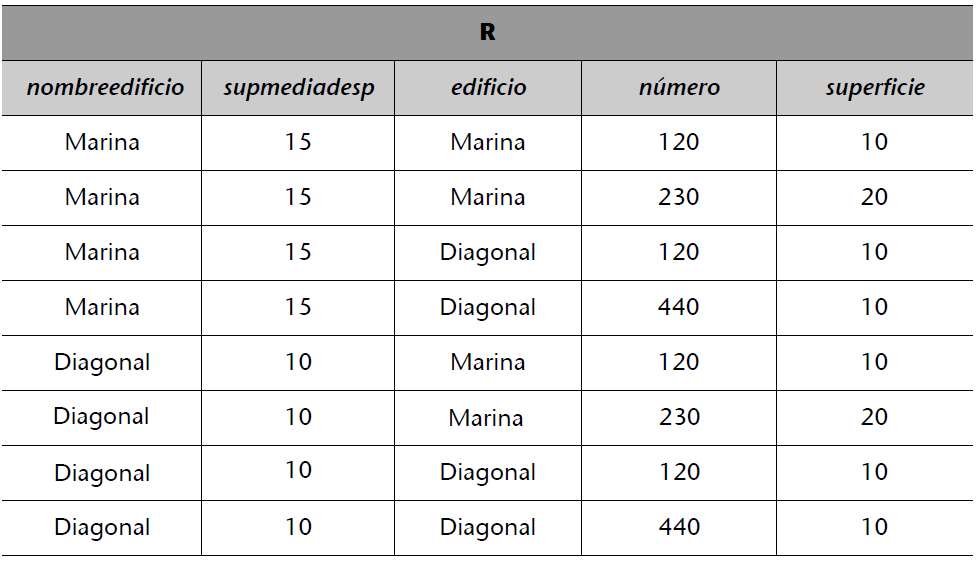
\includegraphics[width=10cm]{imagenes/15_ejemplo7.png}
%\caption{Restultado gr�fico de un producto cartesiano}
%\label{fig:ejemplo7}
%\end{figure}

\begin{table}[h!]
\footnotesize
\centering
\begin{tabular}{|c|c|c|c|c|}
\hline
\multicolumn{5}{|c|}{\textbf{R}}                                                                            \\ \hline
\textit{nombreedificio} & \textit{supmediadesp} & \textit{edificio} & \textit{numero} & \textit{superficie} \\ \hline
Marina                  & 15                    & Marina            & 120             & 10                  \\ \hline
Marina                  & 15                    & Marina            & 230             & 20                  \\ \hline
Marina                  & 15                    & Diagonal          & 120             & 10                  \\ \hline
Marina                  & 15                    & Diagonal          & 440             & 10                  \\ \hline
Diagonal                & 10                    & Marina            & 120             & 10                  \\ \hline
Diagonal                & 10                    & Marina            & 230             & 20                  \\ \hline
Diagonal                & 10                    & Diagonal          & 120             & 10                  \\ \hline
Diagonal                & 10                    & Diagonal          & 440             & 10                  \\ \hline
\end{tabular}
\caption{Restultado gr�fico de un producto cartesiano.}
\label{tab:ejemplo7}
\end{table}


Se debe se�alar que el \textbf{producto cartesiano} es un operaci�n que raramente se utiliza de forma expl�cita, ya que el resultado carece de significado. A pesar de esto, se incluye en el \textit{�lgebra Relacional} porque es una operaci�n primitiva; a partir de la cual se define otra operaci�n que se utiliza con frecuencia llamada \textbf{reuni�n} \cite{campus2006,elmasri2002fundamentos}. \\

\subsection{Reuni�n}
\label{reunion}

La operaci�n \textbf{reuni�n} sirve para combinar tuplas relacionadas de dos relaciones en una sola tupla. Esta es una operaci�n muy importante en cualquier base de datos relacional, ya que \textit{``permite procesar los v�nculos entre las relaciones''} \cite{elmasri2002fundamentos}. \\

De forma general, una \textbf{reuni�n} con dos relaciones $R(A_{1}, A_{2}, ..., A_{n})$ y $S(B_{1}, B_{2}, ..., B_{m})$ se denota como se muestra en la Consulta \ref{eq:31}. \\

\begin{equation}
R\bowtie_{<condicion\_de\_reunion>}S
\label{eq:31}
\end{equation}
\\

El resultado de la \textbf{reuni�n} es una relaci�n $Q$ con $n + m$ atributos $Q(A_{1}, A_{2}, ..., A_{n}, B_{1}, B_{2}, ..., B_{m})$ en ese orden. $Q$ tienen una tupla por cada combinaci�n de tuplas, siempre que �sta satisfaga la condici�n de reuni�n. La condici�n de reuni�n se especifica en t�rminos de atributos de $R$ y $S$, y se eval�a para cada combinaci�n de tuplas. Cada combinaci�n que cumpla con dicha condici�n, se incluir� en la relaci�n resultante $Q$ como una sola tupla \cite{elmasri2002fundamentos}. \\

El tratamiento de la condici�n de reuni�n es id�ntico a la condici�n de selecci�n explicada en la Secci�n \ref{selec}, con la diferencia que la comparaci�n se hace entre atributos de $R$ y $S$. \textit{``Una \textbf{reuni�n} con una condici�n de reuni�n general c�mo �sta se denomina \textbf{reuni�n theta}''} \cite{elmasri2002fundamentos}. \\

Por ejemplo, si se desea encontrar los datos de los despachos que tienen una superficie mayor o igual que la superficie de los despachos del edificio donde est�n situados, entonces se utiliza la operaci�n \textbf{reuni�n} como se muestra en la Consulta \ref{eq:32.1} y \ref{eq:32.2}. \\

\begin{equation}
\rho_{nombreedificio,supmediadesp}\emph{EDIFICIOS\_EMP}
\label{eq:32.1}
\end{equation}
\\
\begin{equation}
\emph{EDIFICIOS\_EMP} \bowtie_{nombreedificio = edificio \wedge supmediadesp \leq superficie}\emph{DESPACHOS}
\label{eq:32.2}
\end{equation}
\\

El resultado gr�fico de la Consulta \ref{eq:32.1} y \ref{eq:32.2} se aprecia en la Tabla \ref{tab:ejemplo8}. Para realizar esta operaci�n, fue necesario cambiar el nombre del atributo $edificio$ de la relaci�n $\emph{EDIFICOS\_EMP}$ por $nombreedificio$, para que no haya problema con el atributo $edificio$ de la relaci�n $\emph{DESPACHOS}$. \\

%\begin{figure}[h!]
%\centering
%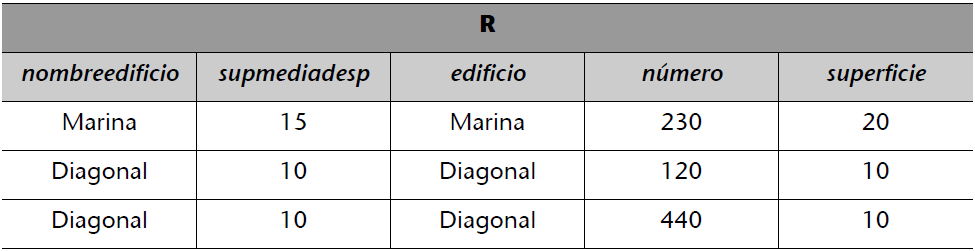
\includegraphics[width=10cm]{imagenes/16_ejemplo8.png}
%\caption{Restultado gr�fico de una reuni�n}
%\label{fig:ejemplo8}
%\end{figure}

\begin{table}[h!]
\footnotesize
\centering
\begin{tabular}{|c|c|c|c|c|}
\hline
\multicolumn{5}{|c|}{\textbf{R}}                                                                            \\ \hline
\textit{nombreedificio} & \textit{supmediadesp} & \textit{edificio} & \textit{numero} & \textit{superficie} \\ \hline
Marina                  & 15                    & Marina            & 120             & 10                  \\ \hline
Diagonal                & 10                    & Diagonal          & 120             & 10                  \\ \hline
Diagonal                & 10                    & Diagonal          & 440             & 10                  \\ \hline
\end{tabular}
\caption{Restultado gr�fico de una reuni�n.}
\label{tab:ejemplo8}
\end{table}

La \textbf{reuni�n} m�s utilizada contiene condiciones de comparaci�n de igualdad exclusivamente. A este tipo de reuni�n se le denomina \textbf{equirreuni�n}. Los resultados de una \textbf{equirreuni�n} siempre tiene uno o m�s pares de atributos con valores id�nticos en todas las tuplas, como se aprecia en la tabla \ref{tab:ejemplo8}, donde los valores de $nombreedificio$ y $edificio$ son iguales para cada tupla. Para evitar esto, se ha especificado otro tipo de operaci�n llamada \textbf{reuni�n natural} \cite{elmasri2002fundamentos}. \\

Una \textbf{reuni�n natural}, se denota como se muestra en la Consulta \ref{eq:33}. \\

\begin{equation}
R \ast S
\label{eq:33}
\end{equation}
\\

Donde $\ast$ es el operador de \textbf{reuni�n natural}, y $S$ y $R$ son relaciones que contengan al menos un atributo con el mismo nombre que se deseen reunir; sirve para deshacerse del segundo atributo que se repite en una condici�n de \textbf{equirreuni�n} \cite{elmasri2002fundamentos}. \\

Como los atributos sobre los cuales se especifica la \textbf{reuni�n natural} tienen los mismos nombre en ambas relaciones, no hace falta renombrarlos. �sto evita el trabajo hecho en los ejemplos de las Tablas \ref{tab:ejemplo7} y \ref{tab:ejemplo8}, donde se debi� cambiar el nombre del atributo $edificio$ de la relaci�n $\emph{EDIFICIOS\_EMP}$ para que no genere un problema con el atributo $edificio$ de la relaci�n $\emph{DESPACHOS}$ \cite{elmasri2002fundamentos}. \\

Por ejemplo, si se hace una \textbf{reuni�n natural} entre $\emph{EDIFICIOS\_EMP}$ y $\emph{DESPACHOS}$, sin la necesidad de renombrar los atributos, se escribe como se muestra en la Consulta \ref{eq:34}. \\

\begin{equation}
\emph{EDIFICIOS\_EMP} \ast \emph{DESPACHOS}
\label{eq:34}
\end{equation}
\\

El resultado gr�fico de la Consulta \ref{eq:34} se aprecia en la Tabla \ref{tab:ejemplo9}. \\

%\begin{figure}[h!]
%\centering
%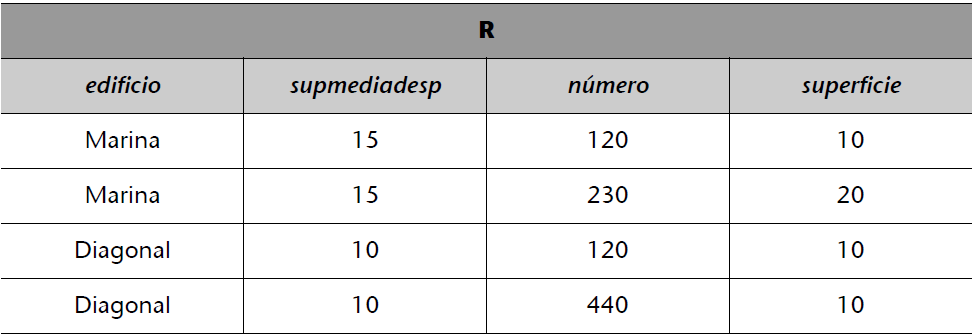
\includegraphics[width=9cm]{imagenes/17_ejemplo9.png}
%\caption{Restultado gr�fico de una reuni�n natural}
%\label{fig:ejemplo9}
%\end{figure}

\begin{table}[h!]
\footnotesize
\centering
\begin{tabular}{|c|c|c|c|}
\hline
\multicolumn{4}{|c|}{\textbf{R}}                                                  \\ \hline
\textit{edificio} & \textit{supmediadesp} & \textit{numero} & \textit{superficie} \\ \hline
Marina            & 15                    & 120             & 10                  \\ \hline
Marina            & 15                    & 230             & 20                  \\ \hline
Diagonal          & 10                    & 120             & 10                  \\ \hline
Diagonal          & 10                    & 440             & 10                  \\ \hline
\end{tabular}
\caption{Restultado gr�fico de una reuni�n natural.}
\label{tab:ejemplo9}
\end{table}

\subsection{Divisi�n}
\label{div}

La operaci�n \textbf{divisi�n} es �til para un tipo especial de consultas que se presenta a veces en aplicaciones de bases de datos. �sta se escribe como se muestra en la Consulta \ref{eq:35}. \\

\begin{equation}
R \div S
\label{eq:35}
\end{equation}
\\

Donde $\div$ es el operador de la \textbf{divisi�n}. �sta se aplica a dos relaciones $R(Z)$ y $S(X)$, d�nde $Z$ es el conjunto de atributos de $R$, $X$ es el conjunto de atributos de $S$ y $X \subseteq Z$. Sea $Y$ el conjunto de atributos de $R$ que no son atributos de $S$, es decir $Y = Z - X$. Para que cada tupla $t$ aparezca en el resultado de $T$ de la \textbf{divisi�n}, los valores de $t$ deben aparecer en $R$ en combinaci�n con todas las tuplas de $S$ \cite{elmasri2002fundamentos}. \\

Si se tiene una relaci�n llamada $\emph{EDIFICIOS\_EMP}$ que contiene s�lo los nombres de los edificios y otra llamada $\emph{EDIFICIOS\_EMPLEADOS}$ que tiene un historial de los edificios en los cuales han trabajado los empleados, ambas se muestran en la Tabla \ref{tab:ejemplo10}. Si se quiere saber cu�les empleados han trabajado en todos los edificios, se hace una \textbf{divisi�n} entre las relaciones $\emph{EDIFICIOS\_EMP}$ y $\emph{EDIFICIOS\_EMPLEADOS}$. El resultado de esta \textbf{divisi�n} se muestra en la Tabla \ref{tab:ejemplo10.1}. Como se aprecia, tanto \textit{Marta} y \textit{Jorge} son valores de $\emph{EDIFICIOS\_EMPLEADOS}(nombre)$ que aparecen en combinaci�n con todas las tuplas de $\emph{EDIFICIOS}(edificio)$. \\

\begin{table}[h!]
\footnotesize
\centering
\begin{tabular}{|c|c|cc}
\cline{1-2}
\multicolumn{2}{|c|}{\textbf{EDIFICIOS\_EMPLEADOS}} &  &                                  \\ \cline{1-2}
\textit{edificio}      & \textit{nombre}     &  &                                  \\ \cline{1-2}
Marina              & Marta             &  &                                  \\ \cline{1-2}
Diagonal              & Marta             &  &                                  \\ \cline{1-2}
Rosales              & Marta             &  &                                  \\ \cline{1-2} \cline{4-4} 
Almodovar              & Marta             &  & \multicolumn{1}{|c|}{\textbf{EDIFICIOS\_EMP}} \\ \cline{1-2} \cline{4-4} 
Marina              & Carlos             &  & \multicolumn{1}{|c|}{\textit{edificio}} \\ \cline{1-2} \cline{4-4} 
Rosales              & Carlos             &  & \multicolumn{1}{|c|}{Marina}         \\ \cline{1-2} \cline{4-4} 
Diagonal              & Elena             &  & \multicolumn{1}{|c|}{Diagonal}         \\ \cline{1-2} \cline{4-4} 
Rosales              & Elena             &  & \multicolumn{1}{|c|}{Rosales}         \\ \cline{1-2} \cline{4-4} 
Almodovar              & Elena             &  &                                  \\ \cline{1-2}
Marina              & Jorge             &  &                                  \\ \cline{1-2}
Diagonal              & Jorge             &  &                                  \\ \cline{1-2}
Rosales              & Jorge             &  &                                  \\ \cline{1-2}
\end{tabular}
\caption{Relaciones $\emph{EDIFICIOS\_EMPLEADOS}$ Y $\emph{EDIFICIOS\_EMP}$.}
\label{tab:ejemplo10}
\end{table}

\begin{table}[h!]
\footnotesize
\centering
\begin{tabular}{|c|}
\hline
\textbf{R} \\ \hline
\textit{nombre} \\ \hline
Marta         \\ \hline
Jorge         \\ \hline
\end{tabular}
\caption{Resultado de una divisi�n.}
\label{tab:ejemplo10.1}
\end{table}

\subsection{Funciones Agregadas y de Agrupaci�n}
\label{funcagreg}

Hay consultas que el �lgebra Relacional no es capaz de responder, por ejemplo obtener el sueldo medio o total de todos los empleados o la cantidad de tuplas existentes en alguna relaci�n. Entre las funciones que suelen aplicarse a colecciones de valores num�ricos est�n \textbf{suma, promedio, m�ximo y m�nimo}. La funci�n \textbf{cuenta} sirve para contar tuplas o valores \cite{elmasri2002fundamentos}. \\

Otra petici�n que se hace con frecuencia es agrupar las tuplas de una relaci�n seg�n el valor de sus atributos y luego aplicar una funci�n agregada independientemente a cada grupo. Por ejemplo, agrupar una relaci�n de empleados por los departamentos a los que pertenecen y luego calcular su sueldo promedio \cite{elmasri2002fundamentos}. \\

Se define una \textbf{funci�n agregada} por el s�mbolo $\mathfrak{F}$ como se muestra en la Consulta \ref{eq:36}: \\

\begin{equation}
_{<atributos\_de\_agrupacion>}\mathfrak{F}_{<lista\_de\_funciones>}(R)
\label{eq:36}
\end{equation}
\\

Donde $atributos\_de\_agrupacion$ es la lista de atributos de $R$,  $lista\_de\_funciones$ es la lista de funciones expresadas de la forma $funcion(atributo)$, donde $funcion$ puede ser una \textbf{suma, promedio, m�ximo, m�nimo} o \textbf{cuenta} y $atributo$ es un atributo de $R$. La relaci�n resultante tiene los atributos de agrupaci�n m�s un atributo por cada elemento de la lista de funciones \cite{elmasri2002fundamentos}. \\

Por ejemplo, si deseamos saber la superficie total por cada edificio en la relaci�n $\emph{DESPACHOS}$, entonces se debe agrupar las tuplas por el atributo $edificio$ y luego calcular la suma del atributo $superficie$ de cada tupla agrupada, como se muestra en la Consulta \ref{eq:37}. \\

\begin{equation}
_{edificio}\mathfrak{F}_{suma(superficie)}(\emph{DESPACHOS})
\label{eq:37}
\end{equation}
\\ 

El resultado gr�fico de la Consulta \ref{eq:37} se muestra en la Tabla \ref{tab:ejemplo12}. \\

\begin{table}[h!]
\footnotesize
\centering
\begin{tabular}{|c|c|}
\hline
\multicolumn{2}{|c|}{\textbf{R}}  \\ \hline
\textit{edificio} & \textit{suma} \\ \hline
Marina            & 30            \\ \hline
Diagonal          & 10            \\ \hline
\end{tabular}
\caption{Resultado de una suma con agrupaci�n de atributos.}
\label{tab:ejemplo12}
\end{table}

Si no se especifica el atributo de agrupaci�n, como se muestra en la Consulta \ref{eq:38}, entonces el resultado ser� el que se muestra en la Tabla \ref{tab:ejemplo13}. \\

\begin{equation}
\mathfrak{F}_{suma(superficie)}(\emph{DESPACHOS})
\label{eq:38}
\end{equation}
\\ 

\begin{table}[h!]
\footnotesize
\centering
\begin{tabular}{|c|}
\hline
\textbf{R}    \\ \hline
\textit{suma} \\ \hline
50            \\ \hline
\end{tabular}
\caption{Resultado de una suma sin agrupaci�n de atributos.}
\label{tab:ejemplo13}
\end{table}

\subsection{Reuni�n Externa}
\label{reuexter}

Las operaciones de \textbf{reuni�n} descritas en la Secci�n \ref{reunion} seleccionan tuplas que satisfacen una condici�n para dicha reuni�n, si las tuplas sin una tupla relacionada o que no satisfagan la condici�n de reuni�n, �stas se eliminan del resultado. Se puede utilizar las \textbf{reuniones externas} cuando se quiera conservar el resultado de todas las tuplas que est�n en alguna de las relaciones que se quiera reunir o en ambas \cite{elmasri2002fundamentos}. \\

La operaci�n \textbf{reuni�n externa izquierda} entre las relaciones $R$ y $S$ denotada por $\leftouterjoin$ conserva todas las tuplas de la \textit{primera relaci�n}, es decir, de $R$. Si no se encuentra alguna tupla coincidente en $S$, los atributos de $S$ en el resultado se rellenan con valores nulos \cite{elmasri2002fundamentos}. Esta operaci�n se muestra en la Consulta \ref{eq:39}. \\

\begin{equation}
R \leftouterjoin S
\label{eq:39}
\end{equation}
\\

Por ejemplo, para hacer una \textbf{reuni�n externa izquierda} entre $\emph{EMPLEADOS\_PROD}$ y $\emph{DESPACHOS}$, renombrando algunos atributos de $\emph{DESPACHO}$, se debe hacer la Consulta \ref{eq:39.1} y \ref{eq:39.2}. Su resultado se muestra en la Tabla \ref{tab:ejemplo14}. \\

\begin{equation}
D \leftarrow \rho_{edificiodesp,numerodesp,superficie}(\emph{DESPACHOS})
\label{eq:39.1}
\end{equation}
\\
\begin{equation}
\emph{EMPLEADOS\_PROD} \leftouterjoin D
\label{eq:39.2}
\end{equation}
\\

\begin{table}[h!]
\footnotesize
\centering
\begin{tabular}{|c|c|c|c|c|c|}
\hline
\multicolumn{6}{|c|}{\textbf{R}}                                                                                            \\ \hline
\textit{ID} & \textit{nombreemp} & \textit{apellidoemp} & \textit{edificiodesp} & \textit{numerodesp} & \textit{superficie} \\ \hline
33.567.711  & Marta              & Roca                 & Marina                & 120                 & 10                  \\ \hline
55.898.425  & Carlos             & Buendia              & Diagonal              & 120                 & 10                  \\ \hline
77.232.144  & Elena              & Pla                  & Marina                & 230                 & 20                  \\ \hline
21.335.245  & Jorge              & Soler                & NULO                  & NULO                & NULO                \\ \hline
88.999.210  & Pedro              & Gonz�lez             & NULO                  & NULO                & NULO                \\ \hline
\end{tabular}
\caption{Resultado de una reuni�n externa izquierda.}
\label{tab:ejemplo14}
\end{table}

La \textbf{reuni�n externa derecha} entre las relaciones $R$ y $S$ denotada por $\rightouterjoin$ conserva todas las tuplas de la \textit{segunda relaci�n}, o sea, de $S$. Si no se encuentra alguna tupla coincidente en $R$, los atributos de $R$ en el resultado se rellenan con valores nulos \cite{elmasri2002fundamentos}. Esta operaci�n se muestra en la F�rmula \ref{eq:40}. \\

\begin{equation}
R \rightouterjoin S
\label{eq:40}
\end{equation}
\\

Por ejemplo, para hacer una \textbf{reuni�n externa izquierda} entre $\emph{EMPLEADOS\_PROD}$ y $\emph{DESPACHOS}$, renombrando algunos atributos de $\emph{DESPACHO}$, se debe hacer la Consulta \ref{eq:40.1} y \ref{eq:40.2}. Su resultado se muestra en la Tabla \ref{tab:ejemplo15}. \\

\begin{equation}
D \leftarrow \rho_{edificiodesp,numerodesp,superficie}(\emph{DESPACHOS})
\label{eq:40.1}
\end{equation}
\\
\begin{equation}
\emph{EMPLEADOS\_PROD} \rightouterjoin D
\label{eq:40.2}
\end{equation}
\\

\begin{table}[h!]
\footnotesize
\centering
\begin{tabular}{|c|c|c|c|c|c|}
\hline
\multicolumn{6}{|c|}{\textbf{R}}                                                                                            \\ \hline
\textit{ID} & \textit{nombreemp} & \textit{apellidoemp} & \textit{edificiodesp} & \textit{numerodesp} & \textit{superficie} \\ \hline
33.567.711  & Marta              & Roca                 & Marina                & 120                 & 10                  \\ \hline
55.898.425  & Carlos             & Buendia              & Diagonal              & 120                 & 10                  \\ \hline
77.232.144  & Elena              & Pla                  & Marina                & 230                 & 20                  \\ \hline
NULO        & NULO               & NULO                 & Diagonal              & 440                 & 10                  \\ \hline
\end{tabular}
\caption{Resultado de una reuni�n externa derecha.}
\label{tab:ejemplo15}
\end{table}

La \textbf{reuni�n externa completa} entre las relaciones $R$ y $S$ denotada por $\fullouterjoin$ conserva todas las tuplas de la \textit{primera relaci�n} y de la \textit{segunda relaci�n}, o sea, de $R$ y $S$. Si no se encuentran tuplas coincidentes, se rellenar�n con valores nulos \cite{elmasri2002fundamentos}. Esta operaci�n se muestra en la F�rmula \ref{eq:41}. \\

\begin{equation}
R \fullouterjoin S
\label{eq:41}
\end{equation}
\\

Por ejemplo, para hacer una \textbf{reuni�n externa completa} entre $\emph{EMPLEADOS\_PROD}$ y $\emph{DESPACHOS}$, renombrando algunos atributos de $\emph{DESPACHO}$, se debe hacer la Consulta que se muestra en la F�rmula \ref{eq:41.1} y \ref{eq:41.2}. Su resultado se muestra en la Tabla \ref{tab:ejemplo16}. \\

\begin{equation}
D \leftarrow \rho_{edificiodesp,numerodesp,superficie}(\emph{DESPACHOS})
\label{eq:41.1}
\end{equation}
\\
\begin{equation}
\emph{EMPLEADOS\_PROD} \fullouterjoin D
\label{eq:41.2}
\end{equation}
\\

\begin{table}[h!]
\footnotesize
\centering
\begin{tabular}{|c|c|c|c|c|c|}
\hline
\multicolumn{6}{|c|}{\textbf{R}}                                                                                            \\ \hline
\textit{ID} & \textit{nombreemp} & \textit{apellidoemp} & \textit{edificiodesp} & \textit{numerodesp} & \textit{superficie} \\ \hline
33.567.711  & Marta              & Roca                 & Marina                & 120                 & 10                  \\ \hline
55.898.425  & Carlos             & Buendia              & Diagonal              & 120                 & 10                  \\ \hline
77.232.144  & Elena              & Pla                  & Marina                & 230                 & 20                  \\ \hline
21.335.245  & Jorge              & Soler                & NULO                  & NULO                & NULO                \\ \hline
88.999.210  & Pedro              & Gonz�lez             & NULO                  & NULO                & NULO                \\ \hline
NULO        & NULO               & NULO                 & Diagonal              & 440                 & 10                  \\ \hline
\end{tabular}
\caption{Resultado de una reuni�n externa completa.}
\label{tab:ejemplo16}
\end{table}

\section{Traducci�n de �lgebra Relacional a SQL}
\label{ar2sql}

Las operaciones del �lgebra Relacional son muy importantes para entender el tipo de solicitudes que podemos especificar en una Base de Datos Relacional. Sin embargo, estas operaciones se consideran \textit{``demasiado t�cnicas para la mayor�a de usuarios de Sistemas Gestores de Bases de Datos Relacionales''}\cite{elmasri2002fundamentos}. \\

Por un lado, las consultas en �lgebra Relacional se escriben secuencialmente, por ende se debe especificar en qu� orden se deben ejecutar las operaciones de consulta. Mientras que SQL proporciona una interfaz de lenguaje declarativo de alto nivel, es decir, el usuario s�lo se preocupa en especificar cu�l es el resultado deseado, dejando que el Sistema Gestor de Base de Datos se preocupe de la optimizaci�n de la consulta y de las decisiones sobre c�mo ejecutarla \cite{elmasri2002fundamentos}. \\

Esta secci�n contiene las transformaciones de las operaciones en �lgebra Relacional a consultas SQL representadas en la Tabla \ref{tab:ar2sql}, donde cada operaci�n tiene su nombre, su sintaxis en �lgebra Relacional y su sintaxis en SQL. \\

\newpage

\begin{table}[h!]
\footnotesize
\centering
\begin{tabular}{|p{3.5cm}|p{4cm}|p{7.5cm}|}
\hline
\rowcolor[HTML]{9B9B9B} 
\multicolumn{3}{|l|}{\cellcolor[HTML]{9B9B9B}\textbf{�lgebra Relacional a SQL}}                                                                                                                                   \\ \hline
\rowcolor[HTML]{C0C0C0} 
\textit{Operador}              & \textit{�lgebra Relacional} & \textit{SQL}                                                                                                                                       \\ \hline
Selecci�n                      & $\sigma_{<condicion>}(r)$                           & \begin{tabular}[c]{@{}l@{}}\texttt{SELECT * FROM \textbf{r}}\\ \texttt{\textbf{WHERE condicion}}\end{tabular}                                                                          \\ \hline
Proyecci�n                     & $\pi_{<lista\_atributos>}(r)$                           & \begin{tabular}[c]{@{}l@{}}\texttt{SELECT}\\ \texttt{\textbf{lista\_atributos}}\\ \texttt{FROM \textbf{r}}\end{tabular}                                                                \\ \hline
Renombrar                      & $\rho_{s(<lista\_atributos>)}(r)$                           & \begin{tabular}[c]{@{}l@{}}\texttt{SELECT * FROM}\\ \texttt{\textbf{r AS s(lista\_atributos})}\end{tabular}                                                                   \\ \hline
Uni�n                          & $r \cup s$                           & \begin{tabular}[c]{@{}l@{}}\texttt{SELECT * FROM \textbf{r}}\\ \texttt{\textbf{UNION}}\\ \texttt{SELECT * FROM \textbf{s}}\end{tabular}                                                                  \\ \hline
Intersecci�n                   & $r \cap s$                           & \begin{tabular}[c]{@{}l@{}}\texttt{SELECT * FROM \textbf{r}}\\ \texttt{\textbf{INTERSECT}}\\ \texttt{SELECT * FROM \textbf{s}}\end{tabular}                                                              \\ \hline
Diferencia                     & $r - s$                           & \begin{tabular}[c]{@{}l@{}}\texttt{SELECT * FROM \textbf{r}}\\ \texttt{\textbf{EXCEPT}}\\ \texttt{SELECT * FROM \textbf{s}}\end{tabular}                                                                 \\ \hline
Producto Cartesiano            & $r \times s$                           & \begin{tabular}[c]{@{}l@{}}\texttt{SELECT * FROM}\\ \texttt{\textbf{r, s}}\end{tabular}                                                                                       \\ \hline
Reuni�n                        & $r \bowtie s$                           & \begin{tabular}[c]{@{}l@{}}\texttt{SELECT * FROM}\\ \texttt{\textbf{r INNER JOIN s}}\end{tabular}                                                                             \\ \hline
Reuni�n Natural                & $r \ast s$                           & \begin{tabular}[c]{@{}l@{}}\texttt{SELECT * FROM} \\ \texttt{\textbf{r NATURAL JOIN s}}\end{tabular}                                                                          \\ \hline
Divisi�n                       & $r \div s$                           & \begin{tabular}[c]{@{}p{7.5cm}@{}}\texttt{SELECT a FROM r}\\ \texttt{WHERE b IN (SELECT b FROM s)}\\ \texttt{GROUP BY A}\\ \texttt{HAVING COUNT (*) = (SELECT COUNT (*) FROM s)}\end{tabular} \\ \hline
Reuni�n Externa Izquierda      & $r \leftouterjoin s$                          & \begin{tabular}[c]{@{}l@{}}\texttt{SELECT * FROM}\\ \texttt{\textbf{r LEFT OUTER JOIN s}}\end{tabular}                                                                        \\ \hline
Reuni�n Externa Derecha        & $r \rightouterjoin s$                           & \begin{tabular}[c]{@{}l@{}}\texttt{SELECT * FROM}\\ \texttt{\textbf{r RIGHT OUTER JOIN s}}\end{tabular}                                                                       \\ \hline
Reuni�n Externa Completa       & $r \fullouterjoin s$                           & \begin{tabular}[c]{@{}l@{}}\texttt{SELECT * FROM}\\ \texttt{\textbf{r FULL OUTER JOIN s}}\end{tabular}                                                                        \\ \hline
\end{tabular}
\caption{Traducci�n de �lgebra Relacional a SQL.}
\label{tab:ar2sql}
\end{table}

\section{Aplicaciones Existentes}
\label{appexist}

En esta secci�n se explicar�n algunas de las herramientas existentes en relaci�n al �lgebra Relacional, finalizando con una tabla comparativa de �stas. \\

\begin{itemize}

\item \textbf{Relational}\footnote{\url{https://github.com/ltworf/relational}} :\\

Consta con una interfaz gr�fica que permite ejecutar consultas tanto directamente por teclado o a trav�s de botones para cada operador, mostrar resultados y guardar, cargar o modificar relaciones en formato CSV o texto plano. Esta herramienta es de c�digo abierto y su repositorio se encuentra disponible para que cualquier persona pueda acceder a �l. Esta disponible para Windows, OS y distribuciones de LINUX. Tiene muy poca documentaci�n y la ayuda que ofrece al usuario para entenderla es bastante reducida, convirti�ndola en una herramienta de dif�cil uso. En la Figura \ref{fig:relational} se muestra un ejemplo de ejecuci�n de esta aplicaci�n.

\begin{figure}[h!]
\centering
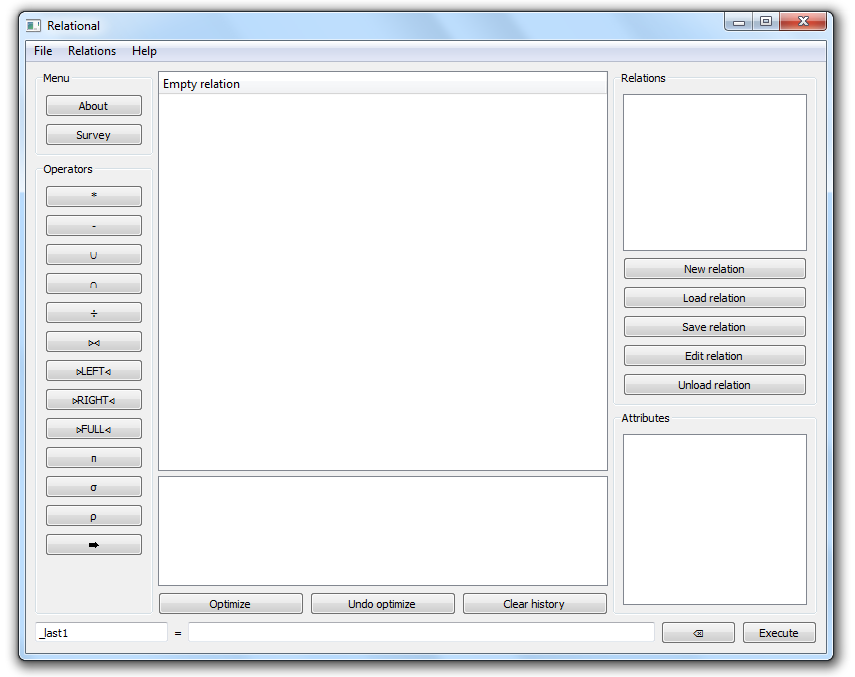
\includegraphics[width=15cm]{imagenes/relational.png}
\caption{Aplicaci�n Relational.}
\label{fig:relational}
\end{figure}

\newpage
\item \textbf{Relational Algebra Translator (RAT)\footnote{\url{http://www.slinfo.una.ac.cr/rat/rat.html}}}: \\

Es una aplicaci�n dise�ada por la Universidad Nacional de Costa Rica y es utilizada ah� para la pr�ctica de sus alumnos en el �lgebra Relacional. Permite escribir y guardar consultas en �lgebra Relacional a trav�s de botones con los operadores o directamente desde teclado, adem�s traduce estas consultas a lenguaje SQL y permite exportar e importar textos en SQL. Permite conexiones a distintas Bases de Datos, pero para �sto es necesario que el usuario tenga instalado y configurado los conectores a las bases de datos que desea acceder; adem�s, no es posible hacer una consulta con la herramienta mientras no est� conectada a alguna base de datos, por lo que su funcionamiento depende enteramente de una base de datos instalada. Es una herramienta multilenguaje (espa�ol, ingl�s, franc�s y alem�n) y con una documentaci�n bastante detallada; s�lo disponible para Windows. En la Figura \ref{fig:rat} se muestra un ejemplo de ejecuci�n.

\begin{figure}[h!]
\centering
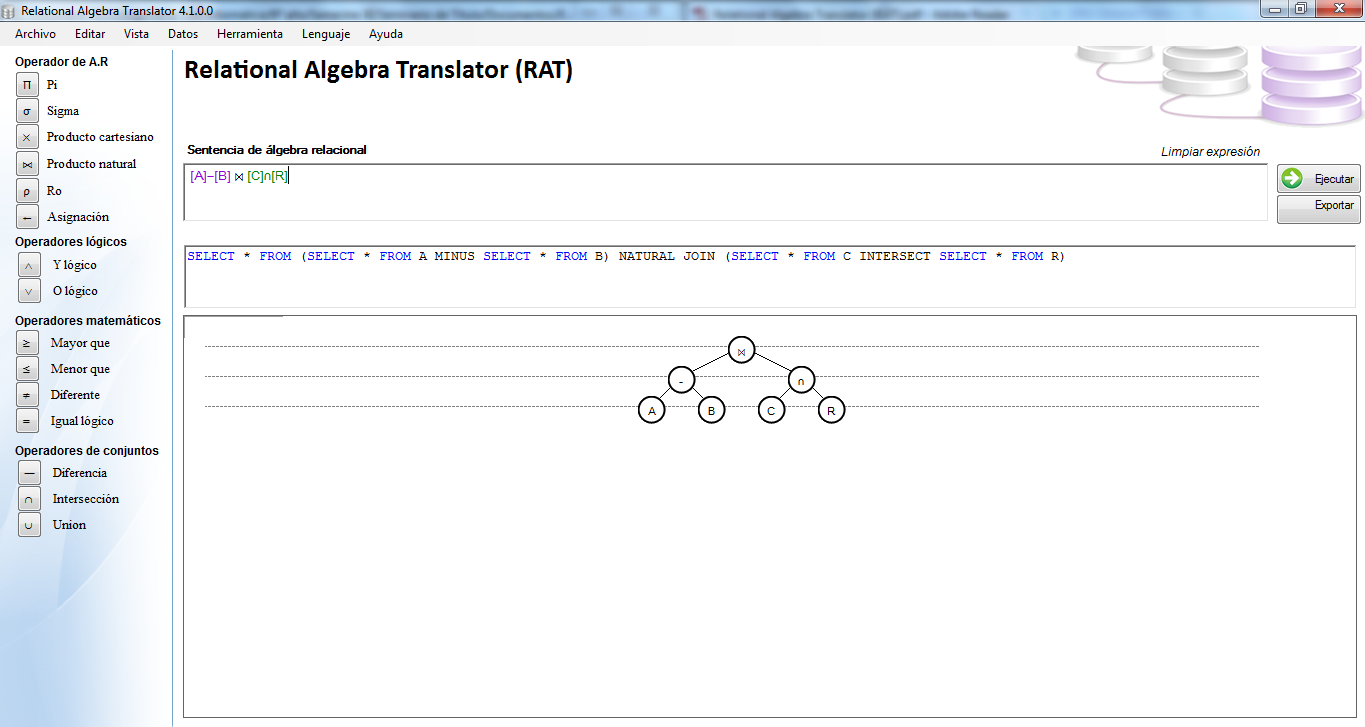
\includegraphics[width=15cm]{imagenes/rat.png}
\caption{Aplicaci�n Relational Algebra Translator (RAT).}
\label{fig:rat}
\end{figure}

\newpage
\item \textbf{WinRDBI\footnote{\url{http://winrdbi.asu.edu/}}}: \\

Es una herramienta para el aprendizaje del �lgebra Relacional desarrollada en Arizona State Universisty. Es multiplataforma, dado que fue programada en JAVA. Contiene una interfaz gr�fica que permite cargar y guardar bases de datos, relaciones y consultas; adem�s de poder cargar dichas relaciones en diferentes formatos. Contiene una documentaci�n muy completa, pero no tiene ayuda directa para la introducci�n de consultas, d�ndole un grado de dificultad a la hora de ingresar expresiones en �lgebra Relacional. Incluye ejemplos de bases de datos y consultas.

\begin{figure}[h!]
\centering
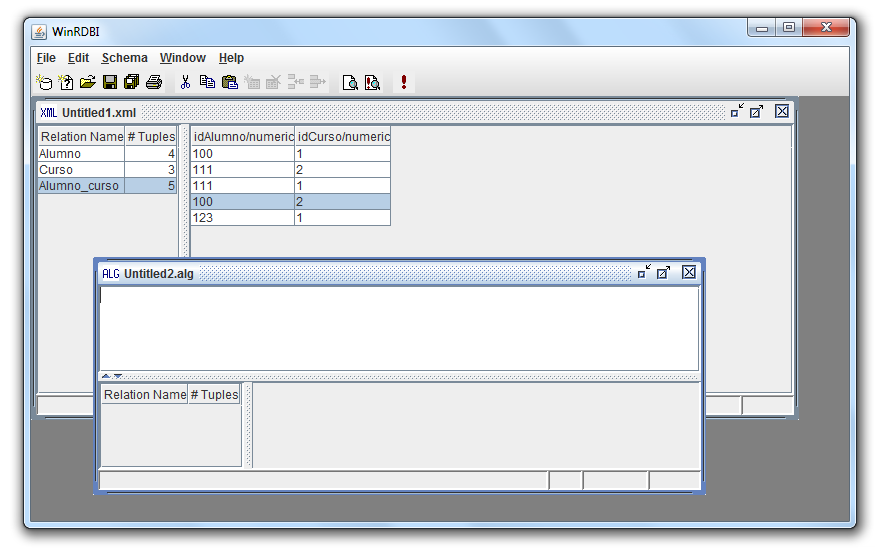
\includegraphics[width=15cm]{imagenes/winrdbi.png}
\caption{Aplicaci�n WinRDBI.}
\label{fig:winrdbi}
\end{figure}

\end{itemize}

\subsection{Comparaci�n entre Herramientas Existentes}

En esta se secci�n se comparan las herramientas explicadas en la Secci�n \ref{appexist}. Se consideran los siguientes aspectos en la comparaci�n:

\begin{itemize}

\item \textbf{Software Libre:} Atributo que indica que la herramienta no tiene costo de adquisici�n. �ste puede ser:

\begin{itemize}
\item S�: No tiene costo de adquisici�n.
\item No: S� tiene costo de adquisici�n.
\end{itemize}

\item \textbf{C�digo Abierto:} Atributo que indica si se tiene o no acceso al c�digo fuente. �ste puede ser:

\begin{itemize}
\item S�: Hay acceso al c�digo.
\item No: No hay acceso al c�digo.
\end{itemize}

\item \textbf{Interoperatibilidad:} Atributo que indica en qu� sistema operativo funciona la herramienta, el cu�l puede ser:

\begin{itemize}
\item W � L � M: Si s�lo funciona para Windows(W), Linux(L) o OS(M).
\item W/L � W/M � L/M: Si funciona con Windows y Linux(WL), Windows y MacOS(WM) o Linux y OS(LM).
\item W/L/M: Si funciona tanto para Windows, Linux y OS.
\end{itemize}

\item \textbf{Interfaz Gr�fica:} Atributo que indica si la aplicaci�n consta de interfaz gr�fica o no. �stos pueden ser:

\begin{itemize}
\item S�: Tiene interfaz gr�fica.
\item No: No tiene interfaz gr�fica.
\end{itemize}

\item \textbf{Ingreso de Consultas:} Atributo que verifica si el ingreso de consultas es directamente v�a teclado o a trav�s de botones:

\begin{itemize}
\item T � B: Si s�lo se pueden hacer consultas a trav�s de teclado(T) o Botones(B).
\item T/B: Si se pueden hacer consultas a trav�s de teclado(T) y botones(B).
\end{itemize}

\item \textbf{Visualizaci�n de Errores:} Atributo que indica si muestra errores sint�cticos en la consulta:

\begin{itemize}
\item S�: Si muestra errores sint�cticos.
\item No: Si no muestra errores sint�cticos. 
\end{itemize}

\item \textbf{Operadores de �lgebra Relacional:} Atributo num�rico que indica la cantidad de operadores de �lgebra Relacional que tiene la aplicaci�n.

\item \textbf{Ayuda para Operadores:} Atributo que indica si la aplicaci�n ofrece ayuda para el uso de los operadores de �lgebra Relacional:

\begin{itemize}
\item S�: Si hay ayuda en todos los operadores.
\item Media: Si hay ayuda en algunos operadores.
\item No: Si no hay ayuda en los operadores.
\end{itemize}

\item \textbf{Lista de Ejercicios:} Atributo que indica si la aplicaci�n tiene problemas en �lgebra Relacional para su ejercitaci�n:

\begin{itemize}
\item S�: si tiene una lista de ejercicios.
\item No: si no tiene una lista de ejercicios.
\end{itemize}

\item \textbf{An�lisis de Datos de quienes usan la Herramienta:} Atributo que indica si la aplicaci�n presenta alguna herramienta para el an�lisis de datos de actividad de los usuarios que utilizan la aplicaci�n:

\begin{itemize}
\item S�: si presenta alguna herramienta para el an�lisis de datos.
\item No: si no presenta alguna herramienta para el an�lisis de datos.
\end{itemize}

\end{itemize}

% Please add the following required packages to your document preamble:
% \usepackage[table,xcdraw]{xcolor}
% If you use beamer only pass "xcolor=table" option, i.e. \documentclass[xcolor=table]{beamer}
\begin{table}[h!]
\footnotesize
\centering
\begin{tabular}{|p{8cm}|p{2.3cm}|p{2.3cm}|p{2.3cm}|}
\hline
\rowcolor[HTML]{9B9B9B} 
\multicolumn{4}{|l|}{\cellcolor[HTML]{9B9B9B}\textbf{Tabla Comparativa ente Aplicaciones}}                           \\ \hline
\rowcolor[HTML]{C0C0C0} 
\textit{Caracter�stica v/s Herramienta}                   & \textit{Relational} & \textit{RAT}    & \textit{WinRDBI} \\ \hline
Software Libre                                            & S�                  & S�              & S�            \\ \hline
C�digo Abierto                                            & S�                  & No              & No         \\ \hline
Interoperatibilidad                                       & WLM                 & W               & W/L/M              \\ \hline
Interfaz Gr�fica                                          & S�                  & S�              & S�               \\ \hline
Ingreso de Consultas                                      & T/B                 & T/B             & T                \\ \hline
Visualizaci�n de Errores                                  & S�                  & S�              & S�               \\ \hline
Operadores de �lgebra Relacional                          & 13                  & 9               & 7                \\ \hline
Ayuda para Operadores                                     & No                  & Media           & No               \\ \hline
Lista de Ejercicios                                       & No                  & No              & No               \\ \hline
\textbf{An�lisis de Datos de quienes usan la Herramienta} & \textbf{No}         & \textbf{No}     & \textbf{No}      \\ \hline
\end{tabular}
\caption{Tabla Comparativa entre Aplicaciones.}
\label{tab:comparacionapp}
\end{table}

\section{Trabajos Existentes}
\label{trabajosexist}

\begin{itemize}

\item \textbf{�lgebra Relacional como lenguaje de acceso a bases de datos relacionales} \cite{valverde1994algebra} : \\

Este trabajo fue publicado en el a�o 1994. En �l se explica la importancia del modelo relacional gracias a su simplicidad a la hora de almacenar datos y la facilidad de acceso a la informaci�n que �ste entrega. Indica tambi�n que su �xito se basa b�sicamente en su fuerte fundamentaci�n te�rica, es decir, la teor�a de conjuntos, el c�lculo matricial y de predicados, entre otros; haciendo que el esquema de tratamiento de informaci�n de este modelo sea bien conocido y probado. Agrega adem�s que el �lgebra Relacional radica la incidencia m�s directa sobre el mundo inform�tico de las bases de datos relacionales. Plantea que algunos lenguajes de manipulaci�n de datos en bases de datos relacionales se han alejado de su inspiraci�n te�rica y proponen una nueva notaci�n para expresar directamente el potencial del �lgebra Relacional en el �mbito de las bases de datos relacionales, ofreciendo un primer acercamiento sobre un SGBD contempor�neo a su �poca llamado DB3 o DBASE III\footnote{\url{http://www.dbase.com}} llamado BAREL\footnote{BAREL: BAse RELational \cite{valverde1994algebra}}. \\

BAREL es un lenguaje de programaci�n que usa operadores en �lgebra Relacional implementados en C y dise�ado como un lenguaje inmerso dentro de la aplicaci�n de DB3. Un lenguaje inmerso es aquel que \textit{"tiene estructura de lenguaje y se apoya, de alguna manera, sobre otro" }\cite{valverde1994algebra}, es decir, debe poder invocar  procedimientos de librer�a del lenguaje anfitri�n y cederles el control, adem�s de permitir el paso de informaci�n a estos procedimientos. De esta forma, cualquier consulta escrita en BAREL podr� ser insertada en un programa para DB3. Antes de que el c�digo fuente original con BAREL inmerso sea ejecutado, �ste debe ser preprocesado para conseguir una traducci�n correcta del mismo. \\

Para el proceso de traducci�n desde el c�digo fuente hasta el ejecutable, se deben llevar a cabo cinco tareas: extracci�n, an�lisis, mezcla, compilaci�n y linkage. En el proceso de extracci�n se extraen s�lo las frases BAREL para reescribirlas en un archivo intermedio. Luego el analizador toma una por una las frases reescritas y les hace un an�lisis l�xico-sint�ctico, en caso de que se adecuen a las reglas gramaticales de BAREL, se genera c�digo para cada una en forma de subf�rmulas algebraicas. Todas estas etapas se llevan a cabo simult�neamente y solo se detiene cuando aparece al menos un error en alguna f�rmula. Despu�s, el mezclador genera un archivo con las frases originales m�s las frases algebraicas sustituidas por sentencias permitidas en DB3. Posteriormente CLIPPER, que es el compilador de DB3, tomar� el archivo anterior y lo compilar� y linkear� para resolver las referencias que se realizan hacia librer�as algebraicas para su posterior ejecuci�n. De esta forma, el usuario podr� convertir textos escritos en DB3 combinados con el lenguaje inmerso BAREL, en programas ejecutables. \\

\item \textbf{Herramienta para la creaci�n y ejecuci�n de consultas en �lgebra Relacional} \cite{velazquez2013herramienta} : \\

El trabajo, en primera instancia recalca la importancia del Modelo Relacional en Bases de Datos, ya que seg�n el texto: \textit{"permite representar la informaci�n del mundo real de una manera intuitiva, introduciendo conceptos cotidianos f�ciles de entender"} \cite{velazquez2013herramienta}, explicando a su vez, cada concepto b�sico necesario para entender este modelo. Indica tambi�n que el �lgebra Relacional es un conjunto de operaciones que permite interactuar con la informaci�n almacenada en una Base de Datos relacional y explica las operaciones que �ste contiene. Adem�s, se�ala que el estudio del �lgebra Relacional es de suma importancia pues: \textit{"ayuda a entender qu� servicios de consultas debe proporcionar un lenguaje relacional, facilita la comprensi�n de algunas de las construcciones de SQL y tambi�n sirve de base para el tratamiento de consultas que efect�an los SGBD internamente"} \cite{velazquez2013herramienta}. Agrega la importancia del aprendizaje del �lgebra Relacional pues los alumnos aprenden de mejor forma si poseen un buen dominio del mismo, indicando que lo ideal seria enfocarse en entender este lenguaje antes de entrar en los detalles particulares de SQL y finalmente recalca la dificultad de ense�anza de este lenguaje ya que seg�n este trabajo: \textit{"es necesario que los estudiantes posean un alto nivel de abstracci�n debido a que no se usa ninguna herramienta que permita realizar pruebas y obtener resultados"} \cite{velazquez2013herramienta}. \\

Por �sto, utilizando C\# y el framework Microsoft .net, se desarroll� una herramienta con interfaz gr�fica que permite la creaci�n y ejecuci�n de c�digo en �lgebra Relacional, ya que las herramientas existentes no son de afines a lo que propone el autor. Los t�rminos empleados son los utilizados en la ense�anza de �lgebra Relacional en su universidad y permite adem�s utilizar una expresi�n que agregue todas las operaciones con sus respectivos par�ntesis o descomponer la expresi�n la expresi�n en varios pasos donde cada uno de ellos explique una operaci�n y su resultado sea utilizado para realizar las operaciones que siguen. \\

\item \textbf{Una herramienta para el aprendizaje del �lgebra Relacional} \cite{hernandez2002herramienta} : \\

Este trabjo indica que el Modelo Relacional se ha establecido como el principal modelo para la construcci�n de Base de Datos, ya que \textit{``consta con fundamentos matem�ticos basados en la teor�a de conjuntos, ayudando al procesamiento eficiente de las consultas en Base de Datos''} \cite{hernandez2002herramienta}. Indica adem�s que uno de los lenguajes para extraer datos de una Base de Datos Relacional es el �lgebra Relacional, agregando tambi�n que el estudio de las Base de Datos Relacionales est� contemplado en el curriculum de su universidad y que presenta una gran falencia, ya que \textit{``se ha demostrado por los docentes que a los alumnos les resulta dif�cil saber que consultas expresadas en papel de �lgebra Relacional son correctas''} \cite{hernandez2002herramienta}, ya que \textit{``esta dificultad se extiende al profesor, al tener que controlar la correcci�n de algunas consultas creativas que a veces se proponen''} \cite{hernandez2002herramienta}. Es por esto que ofrecen una herramienta para el aprendizaje de �lgebra Relacional, ya que a pesar de estar utilizando un prototipo desarrollado en Arizona State University, no se ajusta a los requisitos que ellos plantean. \\

La herramienta construida permite seg�n los autores \textit{``facilitar el aprendizaje de los operadores que constituyen el �lgebra Relacional, combinaciones de operadores para formar consultas, sem�ntica del �lgebra Relacional y sintaxis y sem�ntica de SQL''} \cite{hernandez2002herramienta}. La idea es que en todo momento exista una interactividad entre el alumno y la herramienta dise�ada, de forma que el sistema siempre mantenga informado al usuario de sus errores. El programa contiene un interprete que toma las sentencias de �lgebra Relacional y las transforma en instrucciones SQL para Access\footnote{\url{http://office.microsoft.com/es-hn/access/}} para obtener el resultado de las consultas; un editor visual que se encarga de entregar las herramientas necesarias para crear, editar, compilar y guardar sentencias de �lgebra Relacional y un m�dulo de administraci�n para determinar con qu� base de datos el usuario desea trabajar. Visualmente consta de una barra de operaciones la cual contiene las operaciones de �lgebra Relacional m�s utilizadas y una ventana con tres pesta�as con informaci�n relevante para el usuario como los una descripci�n de los errores que han ocurrido en el proceso de ejecuci�n del programa, las instrucciones SQL resultantes del proceso de compilaci�n de consultas y las tablas de la base de datos con la que se trabaja.\\

\item \textbf{Herramienta para el aprendizaje del �lgebra Relacional y optimizaci�n de consultas} \cite{yuspeirote} : \\

El autor realza la importancia de las Bases de Datos Relacionales en muchos �mbitos de la vida cotidiana. Indica que estas interacciones son finalmente consultas que se hacen a un Sistema Gestor de Base de Datos, y la importancia de realizar estas consultas de forma eficiente hace que el estudio de las Bases de Datos Relacionales sea algo tan imprescindible. Indica que el lenguaje para hacer consultas en un Sistema Gestor de Base de Datos es SQL, pero \textit{``antes de aprender a realizar consultas en este lenguaje es necesario comprender las bases en las que se asienta''} \cite{yuspeirote}, e indica que \textit{``el estudio y la comprensi�n del �lgebra Relacional y sus principio son un aspecto importante en la formaci�n en Base de Datos de los Alumnos de Ingenier�a en Inform�tica''} \cite{yuspeirote}. Por ende, decide generar un herramienta que permita manipular expresiones en �lgebra Relacional, traducirlas a SQL, optimizar consultas y trabajar con ejercicios de ejemplo. \\

Define a grandes rasgos que es el Modelo Relacional, el �lgebra Relacional y explica sus operaciones. A su vez, nombra algunas herramientas existentes durante el desarrollo del trabajo y las compara para dar contraste con la herramienta que desarroll�. Adiciona un Manual de Usuario que contiene una gu�a de instalaci�n del programa y un tutorial completo de c�mo trabajar con la herramienta. Agrega que la herramienta generada es capaz de crear y modificar consultas en �lgebra Relacional a trav�s de una interfaz sencilla e intuitiva, crea y modifica �rboles de expresiones en �lgebra Relacional de una forma visual, ejecuta consultas en la aplicaci�n como en bases de datos externas, optimiza consultas considerando las reglas del �lgebra Relacional, traduce consultas en �lgebra Relacional a SQL e introduce relaciones y tuplas de ejemplo para ejercitar. \\

\end{itemize}

\section{�lgebra Relacional en la Universidad de Valpara�so}
\label{arenuv}

La carrera de Ingenier�a Civil en Inform�tica en la Universidad de Valpara�so es una carrera que dura 12 Semestres y el t�tulo profesional que ofrece es Ingeniero Civil Inform�tico con menci�n en Gesti�n de Software, Gesti�n y Dise�o de Bases de Datos y Redes y Telecomunicaciones. Dentro de su plan de estudios consta con 63. Entre ellas, se encuentra una asignatura que se imparte en el s�ptimo semestre, \textbf{INC402 - Modelo de Datos}. \\


\textbf{INC402 - Modelo de Datos} tiene una duraci�n de 18 semanas y consta de 2 c�tedras por semana de 3 horas cada una, no tiene ayudant�as ni laboratorios para su ejercitaci�n. En ella, se espera que los alumnos sean capaces de entender el papel de las bases de datos dentro de una organizaci�n, y como apoyo a los sistemas de informaci�n presentes en �sta; conocer las fases de ciclo de vida de una base de datos; conocer, analizar y aplicar las distintas t�cnicas de modelamiento de datos. Abarca 5 unidades: Introducci�n a las Bases de Datos, Dise�o de Base de Datos, �lgebra y C�lculo Relacional, Modelo Relacional. La evaluaci�n de esta asignatura consta de 2 cert�menes que equivalen al 60\% de la nota final, 2 controles te�ricos que equivalen al 20\% de la nota final y 1 proyecto dividido en 2 partes que equivale al 20\% de la nota final. El alumno aprueba con una nota igual o superior a 4.0 y reprueba con nota inferior a 3.5; si el alumno obtiene una nota entre 3.5 y 3.9, entonces opta por una prueba especial de toda la materia del curso. En este �ltimo caso, si obtiene una nota igual o superior a 4.0 entonces aprobar� con nota final 4.0, sino reprueba con la nota que se presenta a prueba especial. Es una asignatura de suma importancia ya que es el punta pi� inicial para el estudio de las Bases de Datos, especialmente sobre el modelo Relacional, que de hecho es el fuerte de esta asignatura. \\

La metodolog�a utilizada en esta asignatura son clases te�ricas, apoyada de ejercicios. En ellas, el profesor de c�tedra y a trav�s de clases presenciales, ense�an los conceptos b�sicos que encierran el mundo de las Bases de Datos. Es un ramo muy te�rico, y necesita de mucha pr�ctica para que el alumno sea capaz de entender los conceptos que atiende este curso.\\

La Unidad 4 de esta asignatura es sobre \textbf{�lgebra y C�lculo Relacional} consta de 9 c�tedras y en �l se estudian las operaciones fundamentales, las operaciones extendidas y las funciones agregadas para el �lgebra Relacional. Durante esta etapa, el docente a cargo del curso ense�a y ejemplifica en pizarra los problemas de �lgebra Relacional y los alumnos por su parte ejercitan los problemas de �lgebra Relacional a base de l�piz y papel. Por ende, no poseen herramientas autom�ticas que se adecuen a las necesidades de la universidad para la ense�anza y pr�ctica de ejercicios de �lgebra Relacional. La idea es entregar a este curso una aplicaci�n poderosa y que soluciones los problemas tanto del alumnado para poder ejercitar y obtener resultados inmediatos de sus problemas y consultas en �lgebra Relacional, como para el docente encargado que necesita de una herramienta que sea capaz de decirle d�nde y c�mo se equivocan los alumnos para poder encaminar de mejor manera la asignatura. \\ 

En el Capitulo \ref{problema} se analiza a fondo cu�l es la problem�tica que se presenta en esta asignatura, tanto como profesores como alumnos y se presenta una soluci�n factible y viable que ser� capaz de satisfacer las necesidades del curso. \\




\chapter{Problema}
\label{problema}

\section{Definici�n del Problema}
\label{defproblema}

En esta secci�n se presenta el problema que se tratar� en el presente Trabajo de T�tulo, la soluci�n propuesta para resolver el problema, finalizando con la importancia de �ste. \\

\subsection{Problema}
\label{subproblema}

La Escuela de Ingeniar�a Civil Inform�tica de la Universidad de Valpara�so dentro de su malla curricular contiene una asignatura que se especializa en el conocimiento de las Bases de Datos Relacionales, llamado INC402 - Modelo de Datos. En esta asignatura se ense�a los distintos enfoques de modelos de bases de datos, centr�ndose principalmente en el modelo relacional, c�mo generar modelos relacionales y comprender el tratamiento de consultas mediante el �lgebra Relacional. Es un curso totalmente te�rico y es la base para entender los Sistemas Gestores de Bases de Datos que utilizan Base de Datos Relacionales. Si bien el curso presenta un temario suficiente para comenzar a trabajar directamente con Bases de Datos Relacionales, presenta falencias important�simas a la hora de ense�ar y medir el conocimiento de los alumnos, sobretodo en �lgebra Relacional. \\

Tal como el pseudo-c�digo nos ayuda a entender como trabajar con distintos lenguajes de programaci�n, el �lgebra Relacional es la base de todo Lenguaje Estructurado de Consultas (SQL) y su comprensi�n es de suma importancia al momento de realizar consultas en cualquier Sistema Gestor de Base de Datos. \\

La metodolog�a utilizada para ense�ar el lenguaje se centra en clases presenciales donde se explica qu� es el �lgebra Relacional y c�mo trabajar con �l, ejemplos hechos desde el pizarr�n y gu�as en papel con ejercicios para practicarlo. Esto acarrea una serie de problemas tanto para los alumnos como para el profesor. Uno de ellos es que cuando se realizan ejercicios en papel los alumnos no tienen forma de saber si sus consultas funcionan correctamente, es decir, no saben si su resultado es el deseado o si la sintaxis utilizada es la correcta, oblig�ndolos a esperar hasta encontrarse con alg�n Sistema Gestor de Base de Datos para reci�n probar sus consultas. El profesor por su parte puede formular muchos problemas, guiar el trabajo en clases y entregar una manera correcta de resolverlo, pero los ejercicios realizados por los alumnos fuera de la clase no pueden ser revisados en su totalidad. Herramientas autom�ticas para trabajar con �lgebra Relacional ya est�n implementadas, pero ninguna se adecua a las necesidades de la asignatura, por ende no son utilizadas. Junto con esto, y dado la situaci�n anterior, no existe forma de saber c�mo y en qu� se equivocan los alumnos a la hora de enfrentarse a un problema donde se utilice el �lgebra Relacional fuera del aula. Adem�s, no existe un registro de los errores m�s cometidos ni la frecuencia de los mismos. \\

%\subsection{Enfoque}

\subsection{Soluci�n Propuesta}
\label{solprop}

Este Trabajo de T�tulo tiene como objetivo crear una aplicaci�n que permita trabajar directamente con consultas en �lgebra Relacional, de tal manera que los alumnos de Modelo de Datos de la Escuela de Ingenier�a Civil Inform�tica puedan aprender y ejercitar de forma did�ctica sus consultas en Bases de Datos Relacionales. Junto con �sto, se implementar� un m�dulo de extracci�n de datos con el fin de recopilar informaci�n de entrada ingresada por los alumnos que utilicen la aplicaci�n para as� obtener un feedback m�s representativo y directo a trav�s de alguna t�cnica de Miner�a de Datos. �sta informaci�n tendr� todo tipo de datos del alumno y acciones que ejecute en el programa como errores de consulta, tiempos entre consultas, errores en respuestas de ejercicios, entre otros. Finalmente, por medio de alguna t�cnica de Minar�a de Datos, obtener datos descriptivos de c�mo trabajan los alumnos y cuales son sus errores. \\

\subsection{Importancia del trabajo}
\label{impotrabajo}

Gracias a esto, el alumno podr� detectar de manera inmediata y autom�tica si sus consultas tienen una sintaxis adecuada o si estas entregan los resultados esperados. De esta forma, el alumno se enfocar� directamente en trabajar con �lgebra Relacional y no tendr� la necesidad de enfrentarse directamente con un Sistema Gestor de Base de Datos, evitando la tarea de aprender la sintaxis en lenguaje SQL. \\

Por otra parte, y gracias al sistema de extracci�n de datos, se podr� hacer un seguimiento del trabajo de cada alumno al momento de realizar sus consultas. De esta forma el profesor tendr� la posibilidad de realizar un an�lisis sobre los datos obtenidos con el fin de saber, por ejemplo, cu�les son los errores m�s comunes, la frecuencia de ellos o la cantidad de alumnos que no comenten ning�n error. Esto resulta de mucha ayuda para el profesor, ya que el feedback obtenido gracias al estudio de estos datos puede ser utilizado para reforzar las �reas donde los alumnos presenten m�s problemas, personalizando a�n m�s el aprendizaje de los alumnos. \\

\section{Objetivos}
\label{obj}

En esta secci�n se da a conocer el Objetivo General del Trabajo de T�tulo, junto con los Objetivos Espec�ficos que se desprenden de �l. \\

\subsection{Objetivo General}
\label{objgeneral}

El objetivo principal de este Trabajo de T�tulo es desarrollar una aplicaci�n que ejecute consultas de �lgebra Relacional con el fin de entregar una herramienta did�ctica para fomentar el aprendizaje de este lenguaje, adem�s de construir un m�dulo de extracci�n de datos para el posterior estudio del comportamiento de los alumnos mientras usan la aplicaci�n, mediante alguna t�cnica de Miner�a de Datos, con la finalidad ser un apoyo en la ense�anza del �lgebra Relacional. \\

\subsection{Objetivos Espec�ficos}
\label{objesp}

\begin{itemize}

\item Realizar una toma de requerimientos con el fin de establecer el dominio de trabajo, delimitar la frontera y analizar las necesidades fundamentales que la aplicaci�n debe satisfacer. \\

\item Dise�ar, codificar y testear la aplicaci�n para consultas de �lgebra Relacional. \\

\item Desarrollar una Base de Datos que recopile los datos de las consultas realizadas y conductas de los sujetos de prueba en tiempo de ejecuci�n. \\

\item Crear distintas Bases de Datos de ejemplo para importar a la aplicaci�n a desarrollar. \\

\item Desarrollar un set de ejercicios de ejemplos para cada base de datos de ejemplo. \\

\item Dise�ar, codificar y testear un m�dulo para la captura de datos de las consultas realizadas de los sujetos de prueba en tiempo de ejecuci�n, es decir, errores cometidos, sintaxis, entre otros. \\

\item Utilizando t�cnicas de Miner�a de Datos, analizar e interpretar los datos obtenidos de las pruebas desde la Base de Datos de recolecci�n de informaci�n. \\

\end{itemize}
\chapter{An�lisis}
\label{analisis}

\section{Especificaci�n de Requerimientos}
\label{espreq}

En esta secci�n se presenta los requerimientos que debe satisfacer la aplicaci�n a desarrollar. Estos requerimientos ser�n diferenciados en dos tipos: los requerimientos funcionales que se muestran en la Secci�n \ref{rf} y los requerimientos no funcionales que est�n en la Secci�n \ref{rnf}. \\

\subsection{Requerimientos Funcionales}
\label{rf}

La Tabla \ref{tab:rf} contiene los requerimientos funcionales del sistema. Cada uno contiene un identificador, una descripci�n y un atributo que describe si el requerimiento es obligatorio (O), deseable (D) o prescindible (P). \\

\begin{table}[h!]
\footnotesize
\centering
\begin{tabular}{|p{1cm}|p{13cm}|p{1cm}|}
\hline
\rowcolor[HTML]{9B9B9B} 
\multicolumn{3}{|l|}{\cellcolor[HTML]{9B9B9B}\textbf{Requerimientos Funcionales}}                                                                                                                    \\ \hline
\rowcolor[HTML]{C0C0C0} 
\textit{Id} & \textit{Descripci�n}                                                                                                                                                   & \textit{Tipo} \\ \hline
RF01        & El Programa debe permitir realizar consultas en �lgebra Relacional, es decir, utilizando operadores b�sicos y funciones agregadas.                                     & O             \\ \hline
RF02        & La aplicaci�n debe contar con un set de Base de Datos que sirvan de ejemplo para los alumnos.                                                                          & O             \\ \hline
RF03        & La aplicaci�n debe tener un set de preguntas relacionadas a cada Base de Datos de ejemplo.                                                                             & O             \\ \hline
RF04        & El alumno debe tener la posibilidad de generar relaciones e insertar tuplas en ellas.                                                                                  & D             \\ \hline
RF05        & El alumno puede insertar funciones de consultas en �lgebra Relacional v�a botones presentados en la interfaz gr�fica del programa o directamente desde teclado.        & O             \\ \hline
RF06        & El alumno debe ser capaz de observar gr�ficamente por medio de una tabla el resultado de sus consultas.                                                                & O             \\ \hline
RF07        & El programa debe identificar e informar los errores ocurridos a la hora de ejecutar las consultas ingresadas.                                                          & O             \\ \hline
RF08        & La aplicaci�n debe tener un manual de usuario que explique c�mo utilizar la herramienta.                                                                               & O             \\ \hline
RF09        & La aplicaci�n debe poder guardar alumnos, adem�s de un login para poder ingresar a �l.                                                                                & O             \\ \hline
RF10        & El programa debe ser capaz de guardar y exportar los datos de ingreso y salida de datos de cada consulta durante una sesi�n, es decir, todo lo que realiza el usuario. & O             \\ \hline
RF11        & El programa debe poder transformar las consultas en �lgebra Relacional a Lenguaje SQL.                                                                                 & D             \\ \hline
RF12        & La aplicaci�n debe poder guardar la sesi�n en la que trabaja un alumno.                                                                                                & P             \\ \hline
RF13        & El alumno puede crear sus propias Bases de Datos & D             \\ \hline
RF14        & El programa debe permitir mostrar resultados del trabajo realizado por los alumnos utilizando alg�n algoritmo de Miner�a de Datos.                                     & O             \\ \hline
\end{tabular}
\caption{Requerimientos funcionales del sistema.}
\label{tab:rf}
\end{table}

\subsection{Requerimientos No Funcionales}
\label{rnf}

La Tabla \ref{tab:rnf} contiene los requerimientos no funcionales del sistema. Cada uno contiene un identificador, el atributo de calidad que satisface dicho requerimiento, una descripci�n de �l y un atributo que describe si el requerimiento es obligatorio (O), deseable (D) o prescindible (P). \\

\begin{table}[h!]
\footnotesize
\centering
\begin{tabular}{|p{1.5cm}|p{3cm}|p{9cm}|p{1cm}|}
\hline
\rowcolor[HTML]{9B9B9B} 
\multicolumn{4}{|l|}{\cellcolor[HTML]{9B9B9B}\textbf{Requerimientos No Funcionales}}                                                                                                                                           \\ \hline
\rowcolor[HTML]{C0C0C0} 
\textit{Id} & \textit{Atributo de Calidad} & \textit{Descripci�n}                                                                                                                                              & \textit{Tipo} \\ \hline
RNF 01      & Rendimiento                  & El programa debe tener un tiempo de respuesta no mayor a 5 segundos en carga y creaci�n de relaciones y tuplas.                                                   & D             \\ \hline
RNF 02      & Mantenibilidad               & La plataforma debe contener c�digo debidamente comentado y programado en m�dulos para que se entienda y sea m�s f�cil su mantenci�n. & O             \\ \hline
RNF 03      & Disponibilidad               & La aplicaci�n debe ser una plataforma WEB, con la finalidad de que cualquier alumno o profesor con internet, pueda acceder a �l.                                                                                                                         & O             \\ \hline
RNF 04      & Usabilidad                   & Al usuario no le debe tomar m�s de 1 hora entender las funcionalidades b�sicas del sistema, espec�ficamente: cargar relaciones, hacer consultas y ver resultados. & D             \\ \hline
\end{tabular}
\caption{Requerimientos no funcionales del sistema.}
\label{tab:rnf}
\end{table}

\section{Actores del Sistema}
\label{actores}

Dentro de la aplicaci�n que se desarrollar� para este Trabajo de T�tulo se pueden identificar distintos tipos de usuarios. La Tabla \ref{tab:conusuarios} muestra el nivel de conocimiento que tienen los usuarios que interactuan con la aplicaci�n. \\

\begin{table}[h!]
\footnotesize
\centering
\begin{tabular}{|c|c|}
\hline
\rowcolor[HTML]{9B9B9B} 
\textbf{Nivel de Conocimiento} & \textbf{Descripci�n}                                                       \\ \hline
Experto                        & Usuario con conocimientos avanzados en Bases de Datos y �lgebra Relacional \\ \hline
B�sico                         & Usuario con conocimientos b�sicos en Base de Datos y �lgebra Relacional    \\ \hline
\end{tabular}
\caption{Nivel de conocimiento de los usuarios.}
\label{tab:conusuarios}
\end{table}

La Tabla \ref{tab:usuariossist} contiene los usuarios del sistema, cada uno descrito por un identificador, el nombre de dicho usuario, su nivel de conocimiento y una breve descripci�n de �l. \\

\begin{table}[h!]
\footnotesize
\centering
\begin{tabular}{|p{1.5cm}|p{1.5cm}|p{3cm}|p{7.5cm}|}
\hline
\rowcolor[HTML]{9B9B9B} 
\textbf{Id} & \textbf{Nombre} & \textbf{Nivel de Conocimiento} & \textbf{Descripci�n}                                                                                                                                                                                                                                  \\ \hline
USR 01      & Profesor        & Experto                        & Es el usuario que administra la plataforma. Principalmente es el encargado de permitir y denegar usuarios, generar las bases de datos de ejemplos y ejecutar los algoritmos necesarios para la extracci�n de datos del trabajo hecho por los alumnos. \\ \hline
USR 02      & Alumno          & B�sico                         & Usuario que est� interesado en el estudio del �lgebra Relacional. Su principal tarea es  realizar consultas en �lgebra Relacional y obtener resultado de �stas.                                                                                       \\ \hline
\end{tabular}
\caption{Usuarios del sistema.}
\label{tab:usuariossist}
\end{table}

\newpage

\section{Funciones del Sistema}
\label{funcionessistema}

En esta secci�n se listan las Funciones del Sistema que debe tener las aplicaci�n a desarrollar. Esta lista se muestra en la Tabla \ref{tab:funcionesdelsistema}, donde para cada funci�n se tiene un identificador, una breve descripci�n y atributo que describe si el requerimiento es obligatorio (O), deseable (D) o prescindible (P). \\

\begin{table}[h!]
\footnotesize
\centering
\begin{tabular}{|p{1cm}|p{13cm}|p{1cm}|}
\hline
\rowcolor[HTML]{9B9B9B} 
\multicolumn{3}{|l|}{\cellcolor[HTML]{9B9B9B}\textbf{Funciones del Sistema}}                                                                                    \\ \hline
\rowcolor[HTML]{C0C0C0} 
\textit{Id} & \textit{Descripci�n}                                                                                                              & \textit{Tipo} \\ \hline
F01         & Autorizar las creaciones de cuentas de alumnos y profesores.                                                                      & O             \\ \hline
F02         & Autorizar la modificaciones de cuenta personales de los alumnos y los profesores.                                                 & O             \\ \hline
F03         & Autorizar al profesor la agregaci�n, modificaci�n y eliminaci�n de datos de los alumnos.                                          & O             \\ \hline
F04         & Permitir al profesor la creaci�n, modificaci�n y eliminaci�n de bases de datos.                                                   & O             \\ \hline
F05         & Permitir al profesor la creaci�n, modificaci�n y eliminaci�n de relaciones para cada base de datos.                               & O             \\ \hline
F06         & Permitir al profesor la creaci�n, modificaci�n y eliminaci�n de tupla para cada relaci�n.                                         & O             \\ \hline
F07         & Permitir al profesor la creaci�n, modificaci�n y eliminaci�n de ejercicios y su soluci�n para cada base de datos.                 & O             \\ \hline
F08         & Permitir al alumno la carga de bases de datos.                                                                                    & O             \\ \hline
F09         & Permitir al alumno la creaci�n, modificaci�n y eliminaci�n de sus propias relaciones.                                             & D             \\ \hline
F10         & Permitir al alumno la creaci�n, modificaci�n y eliminaci�n de sus propias tuplas.                                                 & D             \\ \hline
F11         & Permitir al alumno cargar y responder ejercicios de cada base de datos.                                                           & O             \\ \hline
F12         & Permitir a los usuarios ejecutar consultas en �lgebra Relacional, v�a teclado o por medio de botones con cada operador relacional & O             \\ \hline
F13         & Permitir la visualizaci�n del resultado de las consultas.                                                                         & O             \\ \hline
F14         & Permitir la visualizaci�n de errores, si es que existen, para cada consulta.                                                      & O             \\ \hline
F15         & Permitir el almacenamiento y carga de la sesi�n en la que trabaja un alumno.                                                      & D             \\ \hline
F16         & Permitir el almacenamiento de datos de la sesi�n en la que trabaja cada alumno.                                                   & O             \\ \hline
F17         & Permitir al profesor la ejecuci�n de un algoritmo de Miner�a de Datos para el estudio de datos de la sesi�n de los alumnos.       & O             \\ \hline
F18         & Permitir al alumno la creaci�n de bases de datos propias     & D            \\ \hline
\end{tabular}
\caption{Funciones del Sistema.}
\label{tab:funcionesdelsistema}
\end{table}

\section{Casos de Usos}
\label{casosdeusos}

Esta secci�n describe el comportamiento del sistema por medio de los Casos de Usos. La Secci�n \ref{modelocasodeusos} contiene el modelo de casos de usos y la Secci�n \ref{casosdeusosext} contiene el detalle de cada caso de uso. \\

\subsection{Modelo de Casos de Usos}
\label{modelocasodeusos}

En la Figura \ref{fig:diagramacasouso} se presenta el Diagrama de Casos de Usos de la aplicaci�n a generar. �ste cuenta con todas las funcionalidades necesarias para satisfacer los requerimientos descritos en la Secci�n \ref{espreq}. \\

\begin{figure}[h!]
\centering
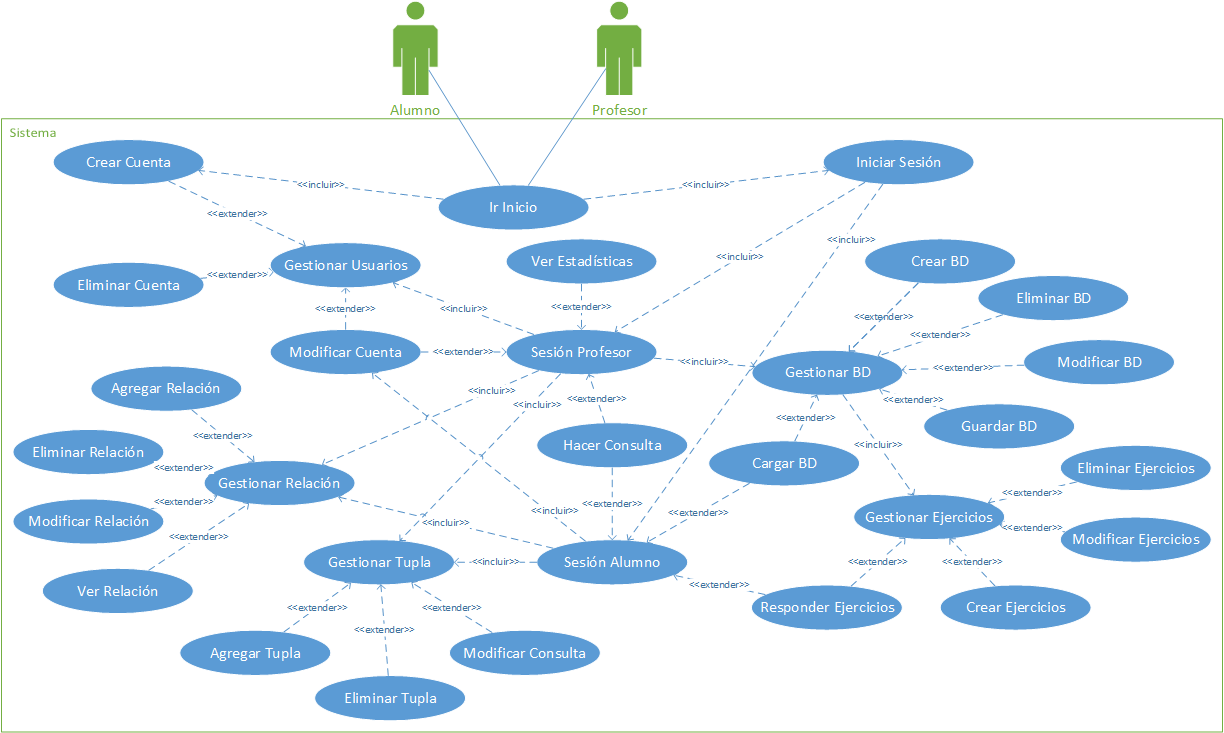
\includegraphics[width=16cm]{imagenes/diagrama_caso_de_uso.png}
\caption{Diagrama de Casos de Usos.}
\label{fig:diagramacasouso}
\end{figure}

\subsection{Casos de Usos Extendidos}
\label{casosdeusosext}

En el Ap�ndice \ref{casosdeusosextendidos} se presentan los casos de Usos Extendidos del Sistema, junto con un diagrama de secuencias y un diagrama de estados. \\

\clearpage
\newpage
\section{Modelo Conceptual}
\label{modeloconceptual}

La Figura \ref{fig:modeloconceptual} muestra el Modelo Conceptual perteneciente a la Aplicaci�n a Desarrollar. En �l se muestran las principales entidades participantes, adem�s de las relaciones que hay entre ellas. \\

\begin{figure}[h!]
\centering
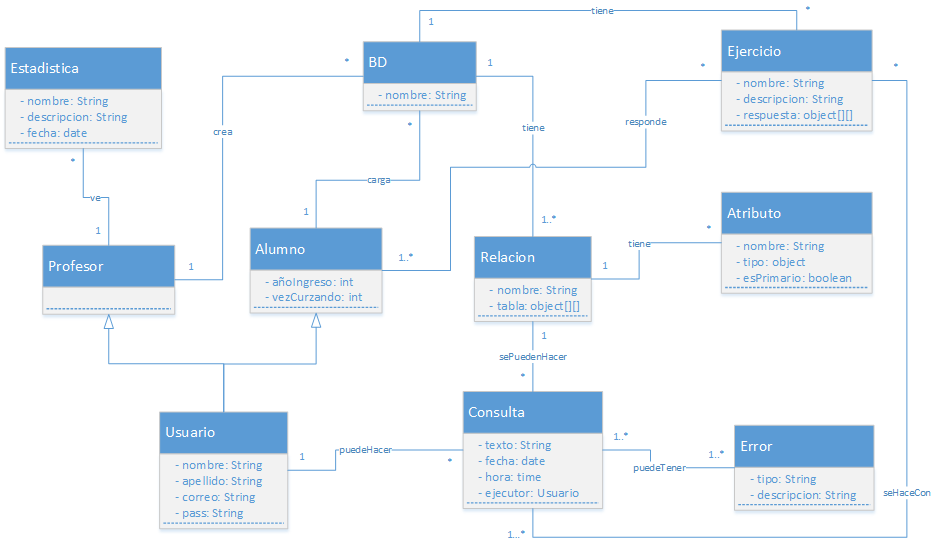
\includegraphics[width=15cm]{imagenes/modelo_conceptual.png}
\caption{Modelo Conceptual.}
\label{fig:modeloconceptual}
\end{figure}
\chapter{Dise�o}
\label{diseno}

El presente cap�tulo corresponde a la descripci�n de la estructura del sistema a desarrollar, el cual considera un conjunto de modelos en distintos niveles de abstracci�n. Estos modelos detallan cada subsistema que lo compone, los datos que manipula y las distintas interfaces que tiene \cite{sommerville2005ingenieria}. \\

Este cap�tulo se divide de la siguiente forma: en la Secci�n \ref{disenoarq} se detalla el Dise�o Arquitect�nico, luego en la Secci�n \ref{disenointerfaz} se define el Dise�o de la Interfaz del Sistema, despu�s en la Secci�n \ref{disenologico} se define el Dise�o L�gico, en la Secci�n \ref{disenodedatos} se muestra el Dise�o de Datos y finalmente en la Secci�n \ref{disenodepruebas} se define el Dise�o de Pruebas. \\

\section{Dise�o Arquitect�nico}
\label{disenoarq}

El Dise�o Arquitect�nico es la primera etapa en el proceso de dise�o de aplicaci�n y \textit{``representa un enlace cr�tico entre los procesos de ingenier�a de dise�o y de requerimientos''} \cite{sommerville2005ingenieria}. \\

La arquitectura presente en la aplicaci�n de este Trabajo de T�tulo es un modelo de 3 capas, debido a que \textit{``soporta el desarrollo incremental de sistemas''} \cite{sommerville2005ingenieria}. �sto es de suma importancia, ya que en primera instancia se puede implementar funcionalidades b�sicas del sistema y luego ir agregando m�s servicios. Adem�s esta arquitectura permite in mejor mantenimiento de la aplicaci�n, gracias a que cada capa se preocupa de un trabajo en espec�fico. Tambi�n, esta arquitectura soporta muy bien los cambios ya que si hace alguna modificaci�n en una capa, �sta impactar� solamente en las capas adyacentes; e incluso si las interfaces de comunicaci�n entre capas no presentan ning�n cambio, una capa puede ser reemplazada por otra equivalente \cite{sommerville2005ingenieria}. \\

\subsection{Modelo de Capas}
\label{modelodecapas}

El Modelo de Capas es una arquitectura que \textit{``organiza el sistema en capas, cada una de las cuales proporciona un conjunto de servicios''} \cite{sommerville2005ingenieria}. La arquitectura que se muestra en la Figura \ref{fig:arquitecturasistema} consta de 3 capas, cada una de ellas posee una responsabilidad dentro del sistema. \\

\begin{itemize}

\item \textbf{Capa Vista:} En esta capa se encuentran todas las interfaces que permiten interactuar con las funcionalidades de la aplicaci�n. Las interfaces presentes en este sistema son: Interfaz de Profesor e Interfaz de Alumno. Esta capa solamente se comunica con la Capa L�gica. \\

\item \textbf{Capa L�gica:} Contiene todas las funcionalidades, operaciones y servicios que ofrece el sistema. En �sta, se recibe y procesan todas las peticiones de usuario provenientes desde la Capa Vista. En caso de ser necesario, �sta se comunicar� con la Capa de Datos para almacenar o recuperar datos. \\

\item \textbf{Capa Datos:} Aqu� se encuentran toda la informaci�n almacenada del sistema. Ac� se almacena y administra los distintos datos de los alumnos, ejercicios, relaciones, entre otros. Esta capa recibe las consultas de recuperaci�n o almacenamiento provenientes desde la Capa L�gica. \\

\end{itemize}

\begin{figure}[h!]
\centering
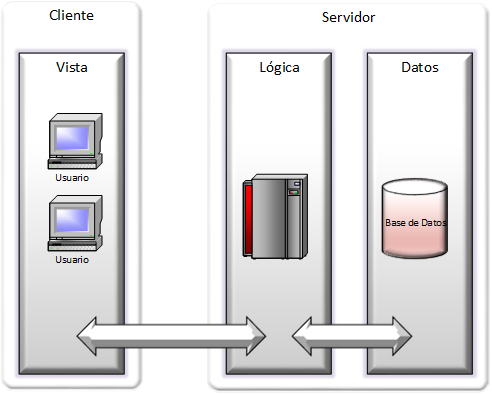
\includegraphics[width=14.5cm]{imagenes/arquitectura_sistema.png}
\caption{Arquitectura del Sistema.}
\label{fig:arquitecturasistema}
\end{figure}

\subsection{Vista de M�dulos}
\label{vistademodulos}

El programa a desarrollar se compone de distintos m�dulos que se muestran en la Figura \ref{fig:vistamodulos}. Cada uno de ellos agrupa una serie de funciones comunes entre s�, lo que permite visualizar todo el sistema modularmente. Los m�dulos que forman parte del sistema son: \\

\begin{figure}[h!]
\centering
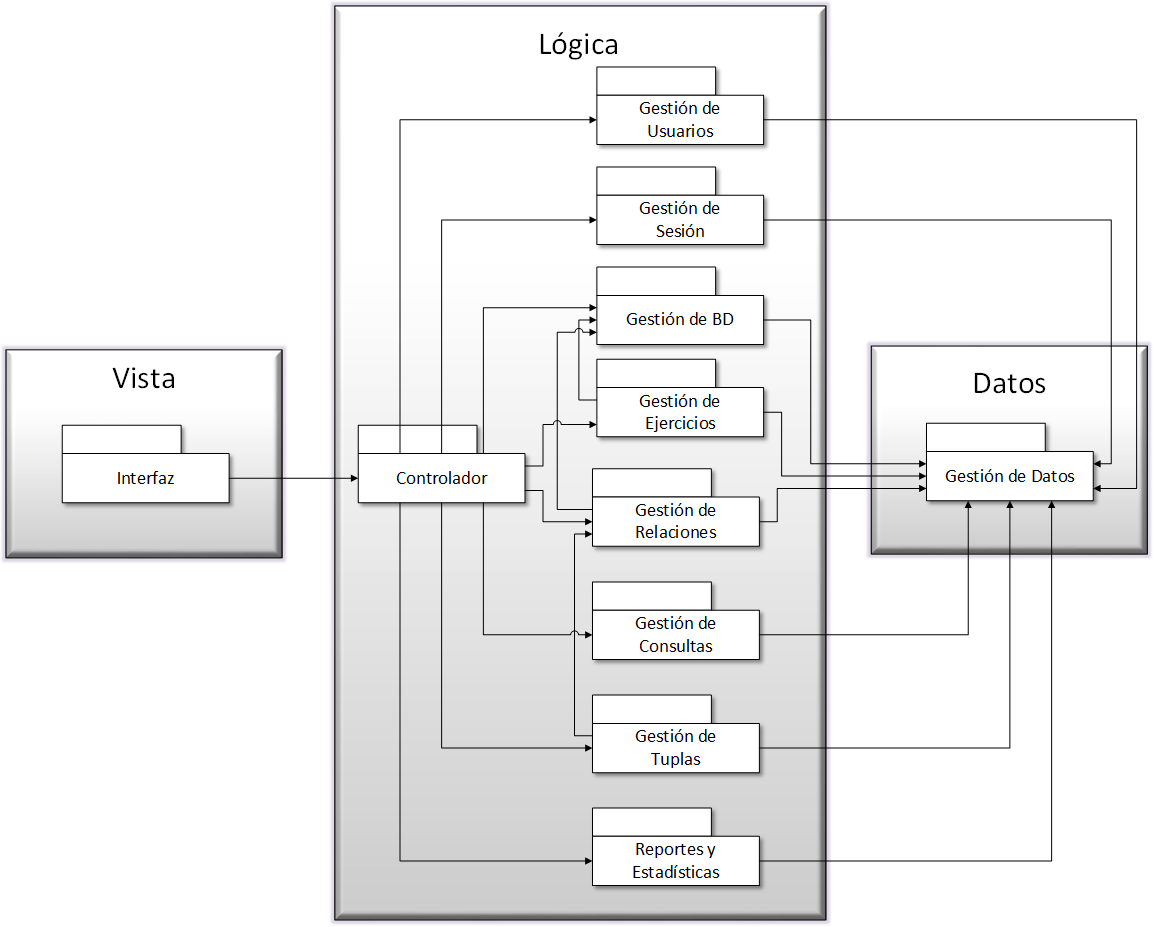
\includegraphics[width=14.5cm]{imagenes/vista_modulos.png}
\caption{Vista de M�dulos y dependencia entre ellos.}
\label{fig:vistamodulos}
\end{figure}

\begin{itemize}

\item \textbf{M�dulo Interfaz:} Contiene todos los componentes y funcionalidades encargadas de la visualizaci�n de las diferentes interfaces para cada tipo de usuario. �stas permiten mostrar al usuario las funcionalidades que tiene el sistema y el resultado de �stas al ser utilizadas. \\

\item \textbf{M�dulo Controlador:} Engloba todos los componentes controladores que reciben peticiones desde la vista y las redirecciona hacia alg�n componente en la capa l�gica que sea capaz de realizar dicha petici�n. Adem�s, este componente es capaz de recibir informaci�n desde la l�gica y enviarla a la capa vista para que sea visualizada por el usuario. \\

\item \textbf{M�dulo Gesti�n de Sesi�n:} M�dulo encargado de la carga y almacenamiento de las sesiones de cada usuario que ingresa al sistema. \\

\item \textbf{M�dulo Gesti�n de Usuarios:} Es el encargado de la creaci�n, eliminaci�n y actualizaci�n de los usuarios que ingresan al sistema. Es importante recalcar que el sistema s�lo permite la gesti�n de alumnos, y la existencia de un �nico profesor admistrador del sistema. \\

\item \textbf{M�dulo Gesti�n de BD:} M�dulo que re�ne todas las funcionalidades que pertenecen a la gesti�n de bases de datos, por ende tiene una dependencia con los m�dulos de Gesti�n de Ejercicios y Gesti�n de Relaciones, debido a que tanto los ejercicios como las relaciones pertenecen a cada base de datos. \\

\item \textbf{M�dulo Gesti�n de Ejercicios:} Engloba todos los componentes relacionados a la creaci�n, modificaci�n y eliminaci�n de ejercicios para cada base de datos en el sistema. \\

\item \textbf{M�dulo Gesti�n de Relaciones:} Contiene las funcionalidades que pertenecen a la creaci�n, modificaci�n y eliminaci�n de relaciones en cada base de datos que est� en el sistema. Debido a que este m�dulo administra las relaciones del sistema, tiene una dependencia con el m�dulo Gesti�n de Tuplas ya que cada tupla pertenece a una relaci�n. \\

\item \textbf{M�dulo Gesti�n de Consultas:} Centraliza todos los componentes dirigidos a la gesti�n de consultas, es decir: ejecuci�n  y verificaci�n de consultas realizadas por usuarios. \\

\item \textbf{M�dulo Gesti�n de Tuplas:} M�dulo que contiene todas las funcionalidades que respectan a la creaci�n, eliminaci�n y modificaci�n de tuplas para cada relaci�n. \\

\item \textbf{M�dulo Reportes y Estad�sticas:} M�dulo encargado de agrupar las funcionalidades que tratan la carga de datos de sesiones de los alumnos y su posterior an�lisis v�a alguna t�cnica de miner�a de datos. \\

\item \textbf{M�dulo Gesti�n de Datos:} Integra las funcionalidades y componentes de la gesti�n de datos hacia la base de datos central del sistema, ya sea para su lectura o actualizaci�n. \\

\end{itemize}



\subsection{Vista de Componentes}
\label{vistadecomponentes}

En la Secci�n \ref{vistademodulos} se definieron y explicaron los m�dulos que componen el sistema. La Figura \ref{fig:vistacomponentes} contiene el modelo de Vista de Componentes del sistema, en �l se aprecian todos los componentes, sus dependencias e interfaces. Cada m�dulo agrupan un conjunto de componentes, los cu�les ser�n descritos a continuaci�n. 


\begin{figure}[h!]
\centering
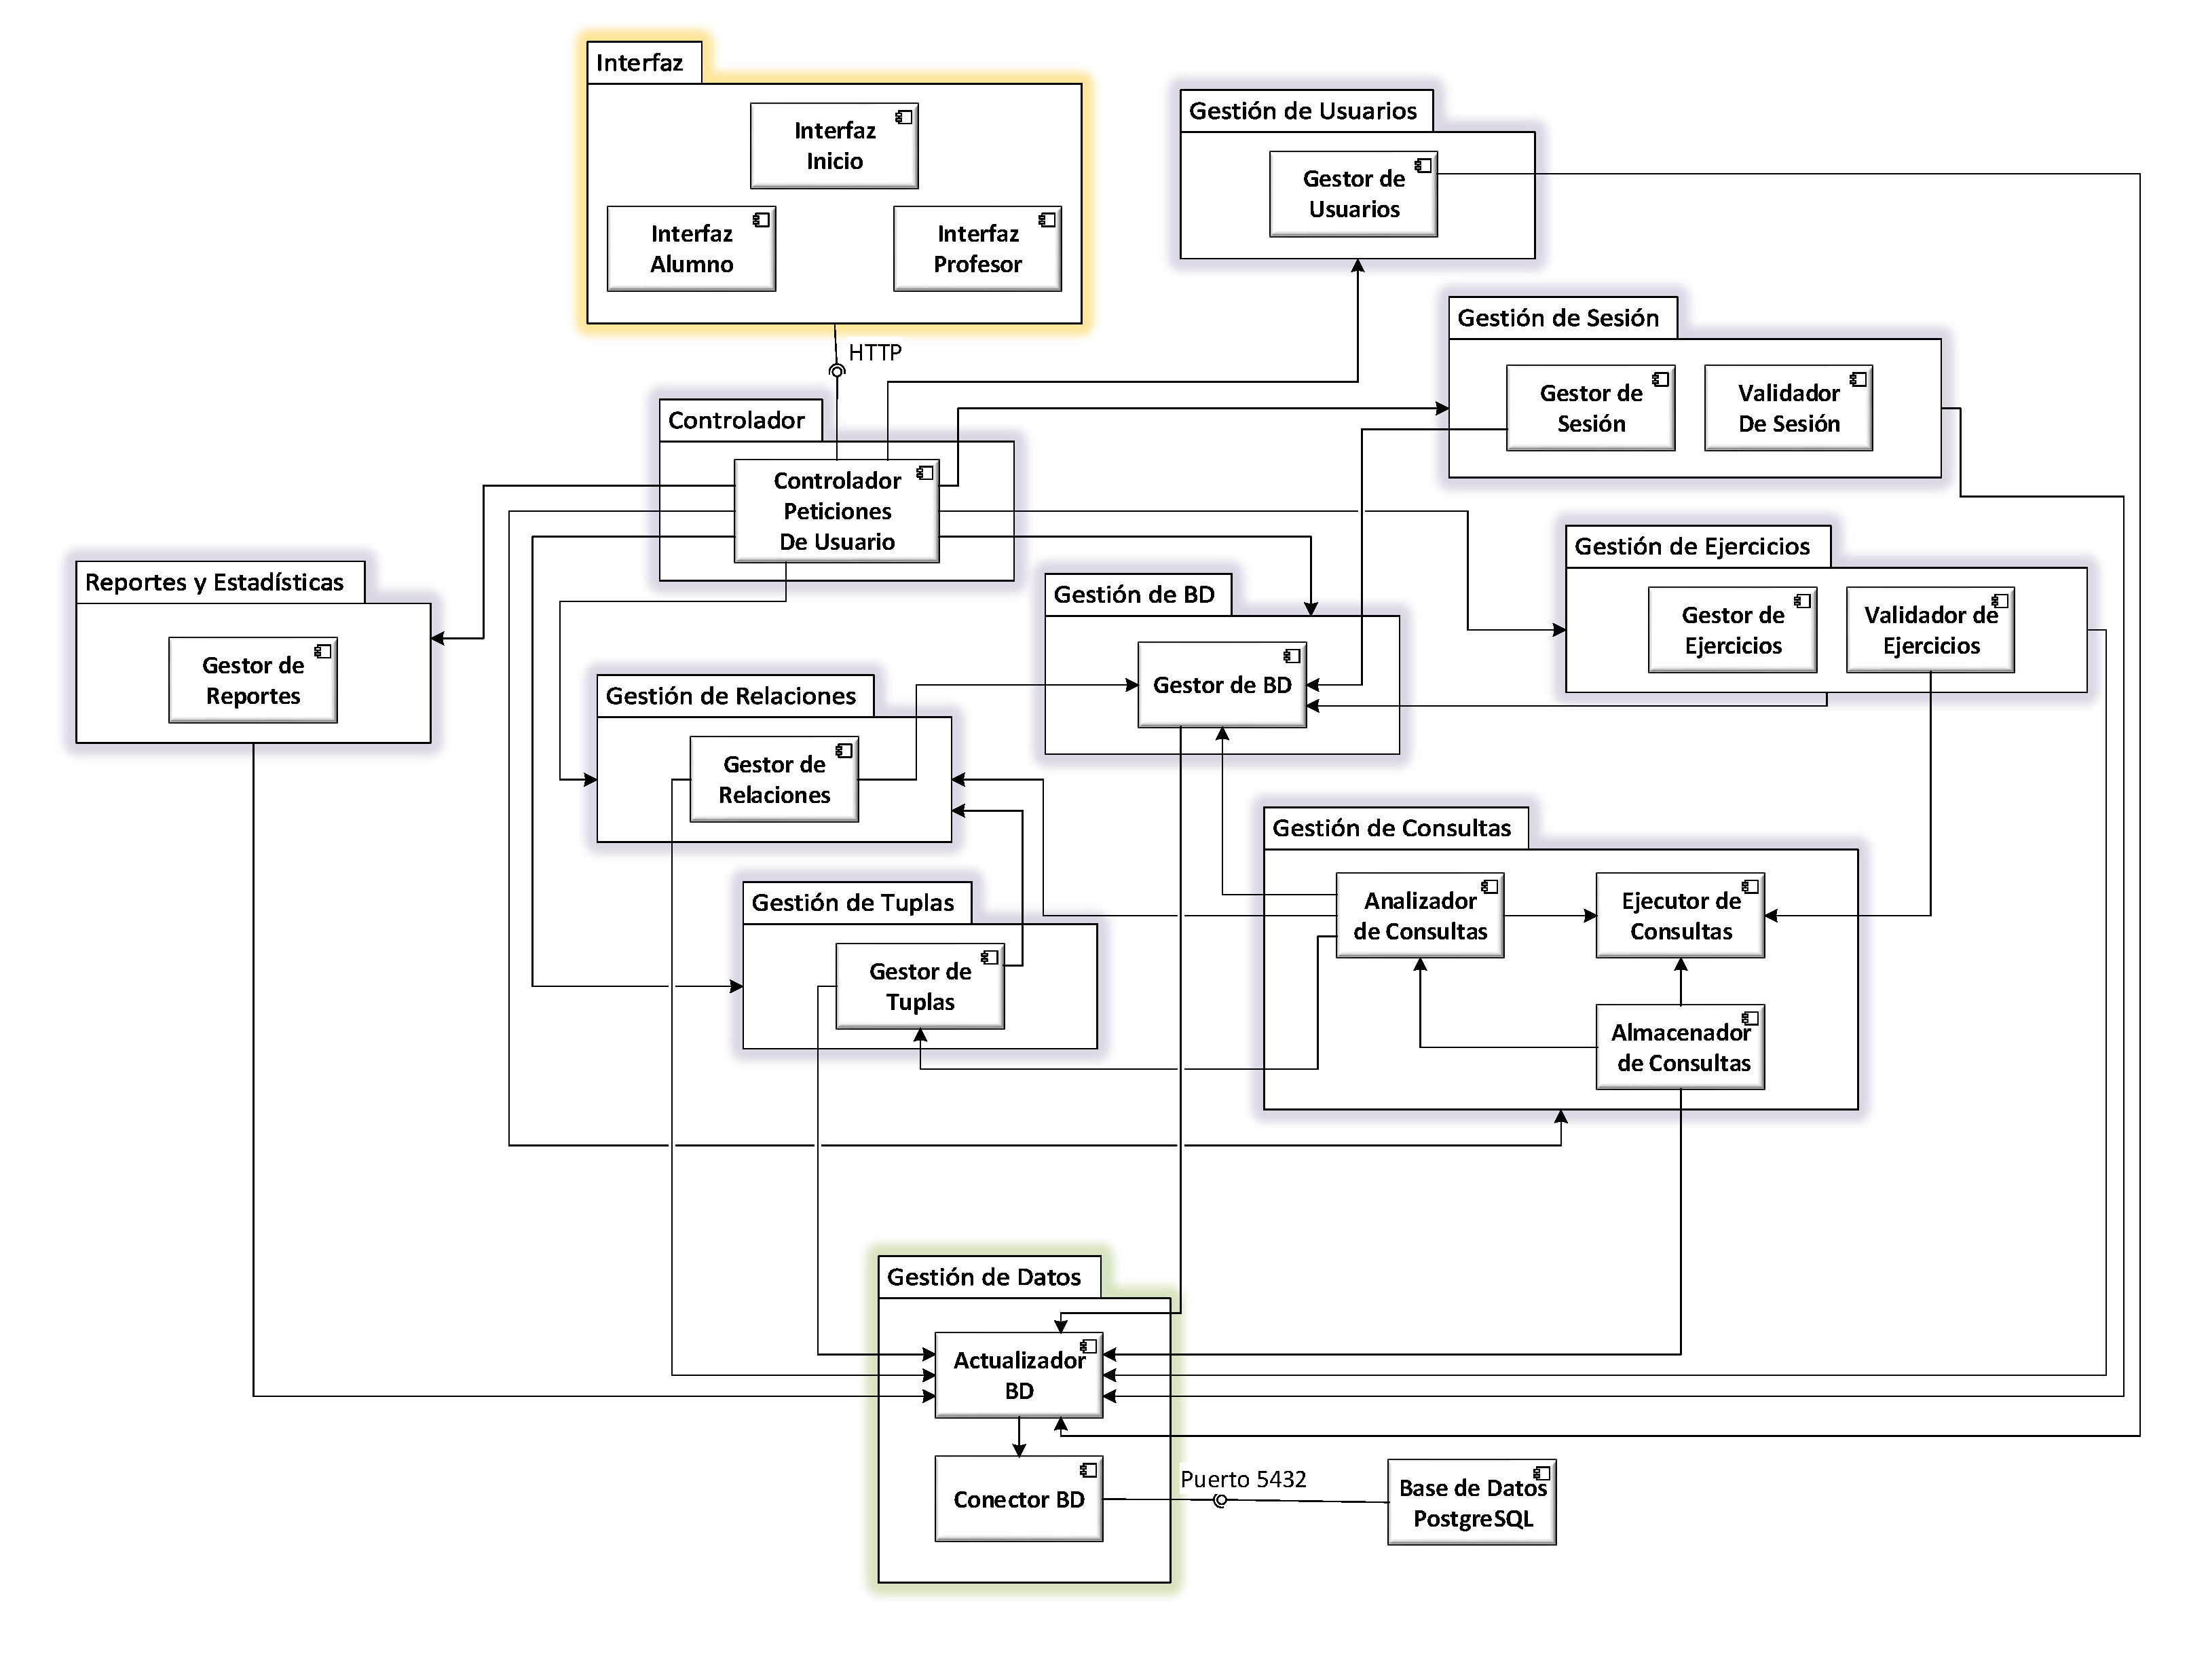
\includegraphics[width=17cm]{imagenes/vista_componentes.pdf}
\caption{Vista de Componentes.}
\label{fig:vistacomponentes}
\end{figure}


\begin{itemize}

\item \textbf{M�dulo Interfaz:} Este m�dulo contiene 3 componentes: \\

	\begin{itemize}

	\item \textbf{Componente Interfaz Inicio:} Este componente contiene la interfaz de inicio y el formulario para identificar a los usuarios, tanto alumno como profesor, que ingresan al sistema. Adem�s, contiene la interfaz para la creaci�n de cuentas, para que los alumnos que entren a la aplicaci�n por primera vez puedan hacer uso de ella. \\
	
	\item \textbf{Componente Interfaz Alumno:} Componente que engloba todas las interfaces de las funcionalidades que un alumno puede utilizar en el sistema. Contiene men�s y formularios, con el fin de acceder a estas funcionalidades de forma interactiva. \\
	
	\item \textbf{Componente Interfaz Profesor:} Componente que engloba todas las interfaces de las funcionalidades que el profesor puede utilizar en el sistema. Contiene men�s y formularios, con el fin de acceder a estas funcionalidades de forma interactiva. \\
		
	\end{itemize}
	
\item \textbf{M�dulo Controlador:} Este m�dulo contiene un componente: \\

	\begin{itemize}

	\item \textbf{Componente Controlador de Peticiones de Usuario:} Este componente contiene recibe las peticiones de los usuarios desde la Interfaz, las procesa y las redirecciona a los m�dulos correspondientes para resolver dicha tarea. \\
		
	\end{itemize}
	
\item \textbf{M�dulo Gesti�n de Usuarios:} Este m�dulo contiene un componente: \\

	\begin{itemize}
	
	\item \textbf{Componente Gestor de Usuarios:} Componente que contiene todas las funcionalidades para procesar los ingresos, modificaciones y eliminaciones de usuarios, espec�ficamente de tipo alumno. Este componente depende del \textit{Actualizador BD} para poder ingresar a la base de datos y poder ejecutar sus funciones. \\	
	
	\end{itemize}
	
\item \textbf{M�dulo Gesti�n de Sesi�n:} Este m�dulo contiene 2 componentes: \\

	\begin{itemize}

	\item \textbf{Componente Gestor de Sesi�n:} Componente encargado de cargar y guardar la sesi�n en la que trabaja el usuario, en espec�fico, las bases de datos generadas por el alumno. Por esto �ltimo, tiene una dependencia al componente \textit{Gestor de BD}. \\
	
	\item \textbf{Componente Validador de Sesi�n:} Este componente se preocupa de la validaci�n de la sesi�n cargada, en otras palabras, de que si los datos ingresados para iniciar la sesi�n son v�lidos. Este componente tiene una dependencia con el componente \textit{Actualizador BD}, ya que a trav�s de �l puede accesar a la base de datos para poder hacer la validaci�n. \\
	
	\end{itemize}
	
\item \textbf{M�dulo Gesti�n de Ejercicios:} Este m�dulo contiene 2 componentes: \\

	\begin{itemize}

	\item \textbf{Componente Gestor de Ejercicios:} Componente que contiene las funcionalidades de guardado, modificaci�n, eliminaci�n y carga de la lista de ejercicios que contiene cada base de datos, por ende tiene una dependencia al componente \textbf{Gestor de BD}. Adem�s, para poder aplicar sus funcionalidades, debe hacer uso del componente \textit{Actualizador BD}. De esta forma, puede hacer uso de la base de datos del sistema. \\
	
	\item \textbf{Componente Validador de Ejercicios:} Componente que agrupa todas las funcionalidades de validaci�n de ejercicios, es decir, que verifica si un ejercicio se responde correctamente o no. �ste tiene una dependencia al componente \textbf{Ejecutor de Consulta}, ya que por medio de una consulta en �lgebra Relacional, se responde un ejercicio. Adem�s, tiene una dependencia con el componente \textit{Actualizador BD}, ya que debe hacer uso de la base de datos del sistema. \\
	
	\end{itemize}
	
\item \textbf{M�dulo Gesti�n de BD:} Este m�dulo contiene un componente: \\

	\begin{itemize}

	\item \textbf{Componente Gestor de BD:} Componente encargado de la carga, guardado, modificaci�n y eliminaci�n de bases de datos de �lgebra Relacional. Este componente tiene una dependencia con el componente \textit{Actualizador BD}, ya que debe hacer uso de la base de datos del sistema para poder ejecutar sus funciones. \\
			
	\end{itemize}
	
\item \textbf{M�dulo Gesti�n de Relaciones: }Este m�dulo contiene un componente: \\

	\begin{itemize}

	\item \textbf{Componente Gestor de Relaciones:} Este componente contiene funciones para guardado, modificaci�n y eliminaci�n de relaciones en una base de datos relacional. �ste componente tiene una dependencia con el componente \textit{Gestor de BD}, ya que a trav�s de �l identifica que relaciones utilizar. Adem�s tiene una dependencia con el componente \textbf{Actualizador BD}, debido al acceso a la base de datos del sistema para poder guardar, modificar o eliminar relaciones. \\
		
	\end{itemize}

\item \textbf{M�dulo Gesti�n de Tuplas: }Este m�dulo contiene un componente: \\

	\begin{itemize}

	\item \textbf{Componente Gestor de Tuplas:} Componente que contiene todas las funciones de carga, ingreso, eliminaci�n y modificaci�n de tuplas en una relaci�n. Este componente tiene una dependencia con el componente \textit{Gestor de Relaciones}, ya que para cada relaci�n existe una lista de tuplas. Adem�s, tiene una dependencia con el componente \textit{Actualizador BD}, ya que debe hacer ingreso a la base de datos del sistema para poder acceder a las tuplas. \\
		
	\end{itemize}
	
	
\item \textbf{M�dulo Gesti�n de Consultas: }Este m�dulo contiene 3 componentes: \\

	\begin{itemize}

	\item \textbf{Componente Analizador de Consultas:} Este componente contiene todas las funcionalidades que respectan a analizar consultas, es decir, la verificaci�n de errores sint�cticos. Dentro de �ste, existe una librer�a llamada ANTLR\footnote{\url{http://www.antlr.org}}, una herramienta para el reconocimiento, elaboraci�n, ejecuci�n y traducci�n de lenguaje estructurado; que por medio de una gram�tica, genera un analizador que puede construir �rboles de an�lisis sint�ctico. \\
	
	\item \textbf{Componente Ejecutor de Consultas:} Componente que contiene las funcionalidades que respectan a la ejecuci�n de consultas, es decir, la definici�n de las consultas en �lgebra Relacional. Tal como el componente \textit{Analizador de Consulta}, utiliza la librer�a ANTLR para la ejecuci�n de las consultas en �lgebra Relacional. \\
	
	\item \textbf{Componente Almancenador de Consultas}	�ste alberga todas las funcionalidades para el almacenamiento de consultas, es decir, si el resultado es correcto en funci�n de un ejercicio, que tipo de errores contiene la consulta, que bases de datos, relaciones o consultas afecta, entre otros. �ste es clave, ya que es el que permite el almacenamiento de datos para su posterior estudio por medio de alguna t�cnica de Miner�a de datos. El Almacenador de consultas depende del \textit{Analizador de Consultas}, ya que de ah� extrae los errores de la consulta, adem�s de donde se ejecuta y del \textit{Ejecutor de Consultas}, ya que de ah� obtiene el resultado de la consulta. Adem�s, tiene una dependencia con el componente \textit{Actualizador BD}, ya que debe hacer ingreso a la base de datos del sistema para poder guardar el resultado de la consulta. \\
	
	\end{itemize}
	
\item \textbf{M�dulo Reportes y Estad�sticas: }Este m�dulo contiene un componente: \\

	\begin{itemize}

	\item \textbf{Componente Resportes y Estad�sticas:} Este componente es el encargado de revisar, verificar y encontrar patrones, por medio de alguna t�cnica de miner�a de datos, de todas las acciones ejecutadas en el sistema, espec�ficamente: tipos de consultas, erroes de consultas, errores en ejercicios, tiempos de respuesta entre ejercicios, entre otros. �ste componente tiene una dependencia con el componente \textit{Actualizar BD}, ya que necesita hacer acceso a la base de datos del sistema, para cargar los datos generados desde el componente \textit{Almacenador de Consultas}. \\
	
	\end{itemize}
	
\item \textbf{M�dulo Gesti�n de Datos: }Este m�dulo contiene 2 Componentes: \\

	\begin{itemize}

	\item \textbf{Componente Actualizador BD:} Componente que engloba todos los accesos a base de datos de todos los componentes del sistema. �ste tiene una dependencia con el componente \textit{Conector BD}, ya que el \textit{Actualizador BD} prepara las consultas y las ejecuta por medio del componente \textit{Conector BD}. \\
	
	\item \textbf{Componente Conector BD:} Este componente contiene la interfaz de acceso a la base de datos. Se encarga de ser el puente conector entre la capa l�gica y la capa de datos, y es el que  tiene acceso directo con la base de datos. \\
	
	\end{itemize}

\end{itemize}

\section{Dise�o Interfaz}
\label{disenointerfaz}

En la presente secci�n, se explicar� como ser� la interfaz de la aplicaci�n. Para ello, en la Secci�n \ref{interfacesdeusuario} se presentan las principales interfaces con la que el usuario trabajar� y en la Secci�n \ref{esquemadenavegacion} se muestra un �rbol de c�mo es la navegaci�n dentro del sistema para cualquier usuario. \\

\subsection{Interfaces de Usuario}
\label{interfacesdeusuario}

En el Ap�ndice \ref{app-interfacesdeusuario} se presentan las principales interfaces del usuario, junto con una explicaci�n de cada uno de ellos. \\

\subsection{Esquema de Navegaci�n}
\label{esquemadenavegacion}

El esquema de navegaci�n presentado en la presente secci�n posee una topolog�a jer�rquica jer�rquica, la que se visualiza al instante de ingresar ordenadamente a las funcionalidades a trav�s de los elementos gr�ficos que contiene la interfaz. Las Figuras \ref{fig:navegacionprofesor} y \ref{fig:navegacionalumno} contienen el modelo de navegaci�n de usuario para Profesor y Alumno respectivamente. \\

\begin{figure}[h!]
\centering
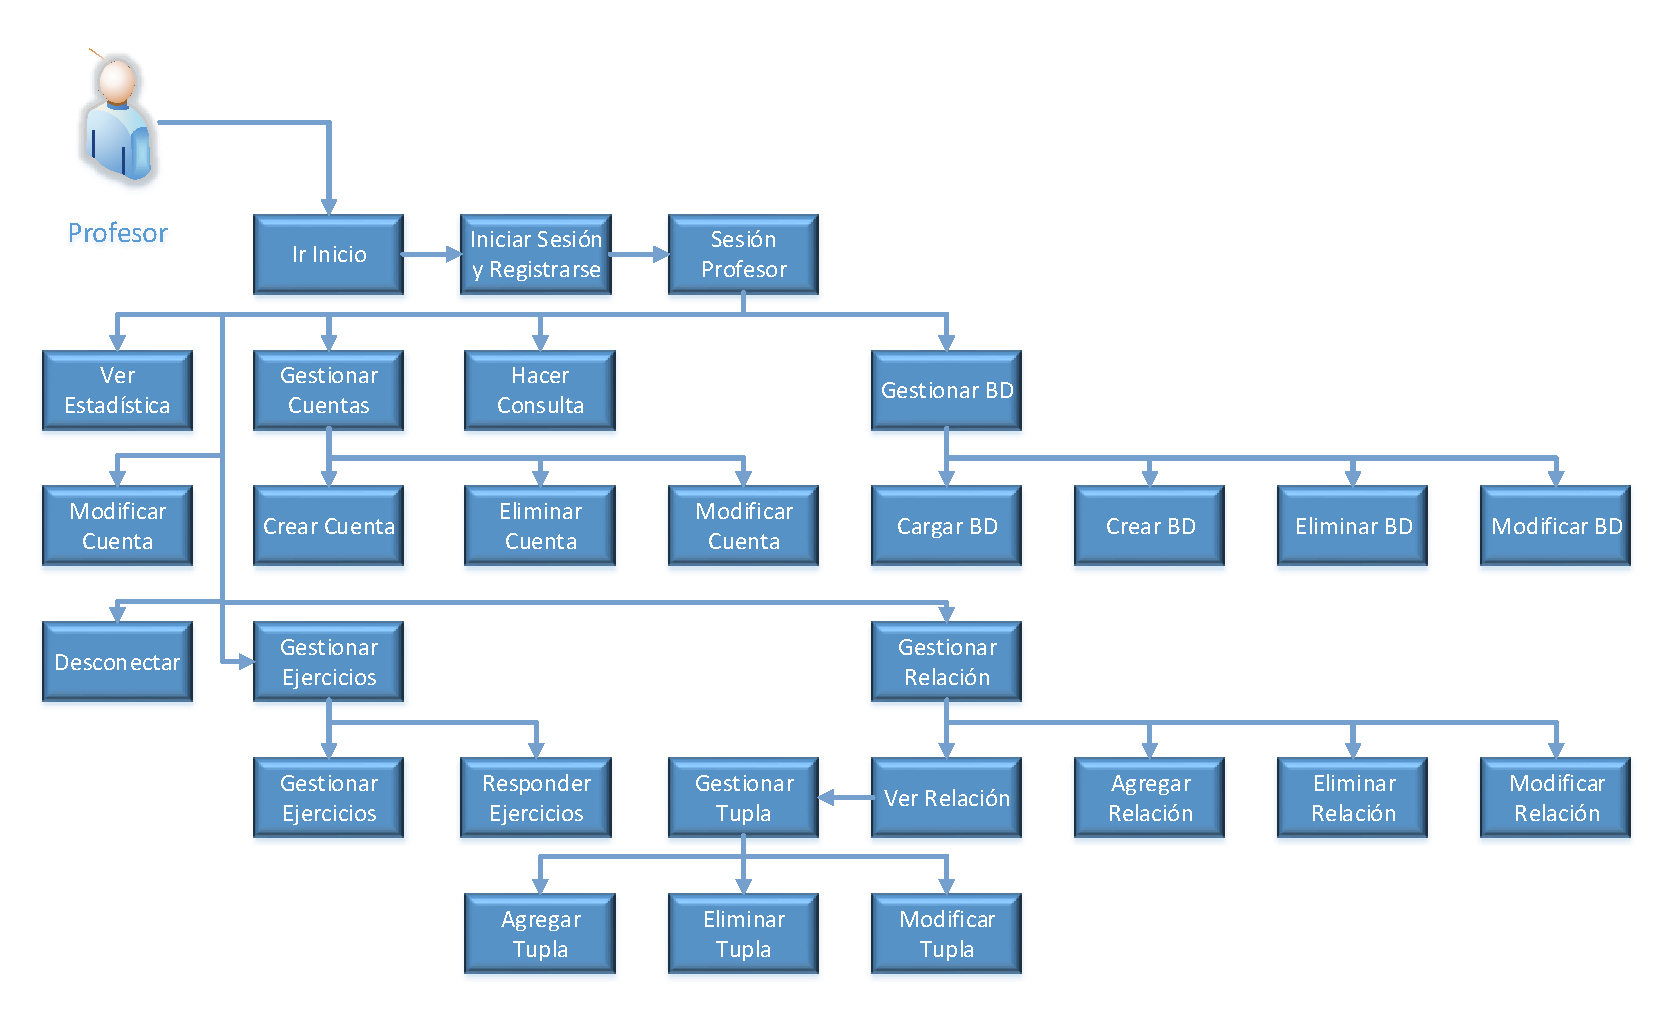
\includegraphics[width=14.5cm]{imagenes/navegacion_profesor.pdf}
\caption{Esquema de Navegaci�n Profesor.}
\label{fig:navegacionprofesor}
\end{figure}

\begin{figure}[h!]
\centering
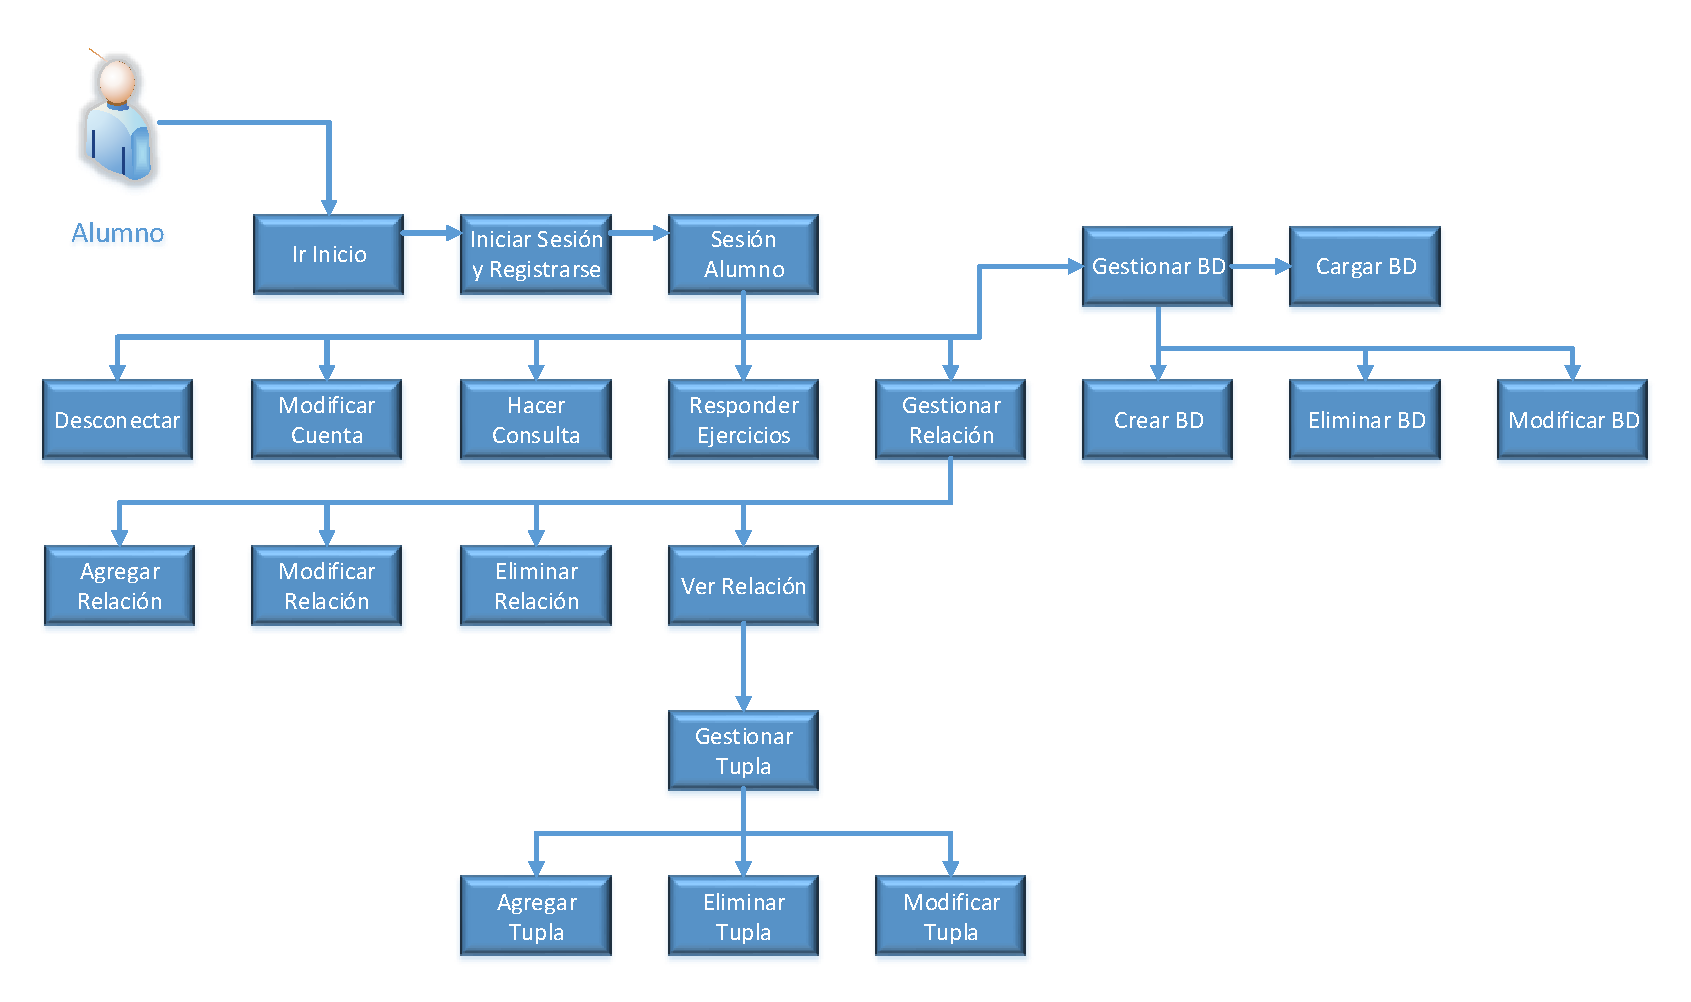
\includegraphics[width=14.5cm]{imagenes/navegacion_alumno.pdf}
\caption{Esquema de Navegaci�n Alumno.}
\label{fig:navegacionalumno}
\end{figure}

\newpage
\section{Dise�o L�gico}
\label{disenologico}

La presente secci�n tiene como objetivo proporcionar la estructura para el desarrollo del sistema. En la Secci�n \ref{casosdeusosreales} se muestran los Casos de Usos Reales y en la Secci�n \ref{diagramadeclases} se define el Diagrama de Clases. \\

\subsection{Casos de Usos Reales}
\label{casosdeusosreales}

En el Ap�ndice \ref{app-casosdeusosreales} se presentan los casos de usos reales de la aplicaci�n, acompa�ados con figuras etiquetadas que explican donde se encuentran las funcionalidades explicada por cada caso de uso real. \\

\subsection{Diagrama de Clases}
\label{diagramadeclases}

En la Figura \ref{fig:diagramadeclases} se presenta el diagrama de clases de la aplicaci�n a desarrollar. Ah� se presentan cada una de las clases implicadas en la funcionalidad del sistema y como interact�an entre ellas. A continuaci�n se muestra una breve explicaci�n de cada clase: \\

\begin{itemize}

\item \textbf{CargarBDBean:} Es la clase controladora encargada de la comunicaci�n entre la interfaz y la l�gica para poder cargar una base de datos seleccionada por un usuario. \\

\item \textbf{CrearCuentaBean:} Clase controladora preocupada de la comunicaci�n entre la interfaz y la capa l�gica para la creaci�n de usuarios alumnos por medio de una sesi�n de profesor. \\

\item \textbf{EliminarCuentaBean:} Clase controladora encargada de la comunicaci�n entre la interfaz y la capa l�gica para la eliminaci�n de cuentas de alumnos por medio de una sesi�n de profesor. \\

\item \textbf{EstadisticasView:} Clase encargada de procesar las estad�sticas cargadas desde la base de datos y enviarlas a la interfaz para que sea visualizadas por el usuario. \\

\item \textbf{GestionarEjerciciosBean:} Clase preocupada de controlar todas las funcionalidades que respectan a la gesti�n de Ejercicios en el sistema desde la capa vista a la capa de negocio. En ella se puede crear, modificar o eliminar distintos ejercicios para alguna base de datos cargada. \\

\item \textbf{HacerConsultaBean:} Es la clase controladora encargada de procesar y comunicar las peticiones entre la interfaz y la capa l�gica para las consultas en el lenguaje de �lgebra Relacional hechas por los usuarios. \\

\item \textbf{LoginBean:} Clase controladora que se preocupa de gestionar, desde la interfaz a la l�gica, las distintas funcionalidades para el inicio de sesi�n y para la creaci�n de cuentas de alumnos. \\

\item \textbf{MenuView:} Clase preocupada controlar los distintos men�s que corresponden a cada usuario. De esta forma, un alumno no puede entrar v�a men� a vistas que son exclusivamente del profesor. \\

\item \textbf{ModificarCuentaBean:} Claase preocupada de controlar todas las funcionalidades que respectan a la eliminaci�n de cuentas de alumno realizadas por un profesor. \\

\item \textbf{ModificarCuentaAlumnoBean:} Clase encargada de todas las funcionalidades de modificaci�n de cuenta del alumno. �sta permite al alumno modificar sus propios atributos en el sistema. \\

\item \textbf{ModificarCuentaProfesorBean:} Clase encargada de todas las funcionalidades de modificaci�n de cuenta del profesor. �sta permite al profesor modificar sus propios atributos en el sistema. \\

\item \textbf{ObtenerCalificacionBean:} Clase controladora encargada de procesar los resultados del alumno y enviarlos a la capa vista para que sea visualizadas, adem�s preparar estos datos para ser guardados en una base de datos. \\

\item \textbf{ResponerEjerciciosBean:} Clase controladora encargada recibir y enviar a interfaz los distintos ejercicios que posee una base de datos. Adem�s, esta clase env�a estos resultados a la clase \textit{ObtenerCalificacionBean} para que sean procesados por �ste. \\

\item \textbf{Util:} Clase encargada de guardar funcionalidades que se constantemente utilizadas por otras clases, entre ellas, obtener las variables de sesi�n activas y recargar una base de datos. \\

\item \textbf{User:} Clase que encapsula los datos del Usuario en el sistema. �sta clase contiene todos los datos del usuario, adem�s de las distintas bases de datos. \\

\item \textbf{Atributo:} Clase que encapsula la informaci�n de los atributos de una relaci�n. \\

\item \textbf{Consulta:} Clase que contiene todos los datos de las consultas realizadas durante la resoluci�n de un ejercicio de alguna base de datos. \\

\item \textbf{Ejercicio:} �sta clase contiene toda la informaci�n de cada ejercicio que contiene una base de datos. \\

\item \textbf{Esquema:} Clase que contiene todos los datos de las bases de datos relacionales en el sistema. Esta clase adem�s contiene todas sus relaciones. \\


\item \textbf{Relacion:} Clase que contiene los datos de cada relaci�n de cualquier base de datos del sistema. Esta clase contiene adem�s una serie de atributos y tuplas que son los que describen cada columna y cada fila de una tabla. \\

\item \textbf{Respuesta:} �sta clase encapsula todos los datos de las respuestas hechas por cada usuario a la hora de responder una gu�a de ejercicios de alguna base de datos. \\

\item \textbf{Resultado:} Clase que engloba todos los datos de las respuestas de cada gu�a de ejercicios de alguna base de datos en el sistema. \\

\item \textbf{Tupla:} Clase que contiene todos los datos de las tuplas de una relaci�n perteneciente a alguna base de datos del sistema. \\

\item \textbf{AlgebraRelacionalLexer:} Clase que contiene los datos relativos a los componentes del lenguaje de �lgebra Relacional, como por ejemplo las palabras reservadas del lenguaje. \\

\item \textbf{AlgebraRelacionalParser:} Clase que ejecuta una consulta y revisa sint�cticamente una consulta realizada en el lenguaje de �lgebra Relacional. �sta indica si la consulta est� v�lida o no. \\

\item \textbf{Database:} Esta clase es la interfaz de conexi�n entre la l�gica y la base de datos. Es de suma importancia, ya que gracias a �sta todas las clases de tipo DAO (Data Acces Object) pueden hacer ingreso a la base de datos del sistema. \\

\item \textbf{ConsultaDAO}: Clase preocupada del almacenamiento de consulta realizadas durante la resoluci�n de un ejercicio a la base de datos del sistema. Se encarga de dar comunicaci�n entre la base de datos y la capa l�gica. \\

\item \textbf{EjercicioDAO:} Clase de acceso a la base de datos del sistema encargada del ingreso, modificaci�n o eliminaci�n de ejercicios de una base de datos. �sta clase es la interfaz de comunicaci�n entre la capa de datos y la capa l�gica. \\

\item \textbf{EsquemaDAO:} Esta clase es la interfaz de comunicaci�n entre la capa de datos y la capa l�gica para el almacenamiento, carga y modificaci�n de esquemas o base de datos en la base de datos del sistema. \\

\item \textbf{RelacionDAO:} Clase preocupada del acceso a base de datos para la recuperaci�n, ingreso o actualizaci�n de relaciones de cada base de datos relacional. Se encarga de dar comunicaci�n entre la base de datos y la capa l�gica. \\

\item \textbf{UserDAO:} Clase de acceso a la base de datos encargada del ingreso, modificaci�n o eliminaci�n de usuarios del sistema. �sta clase es la interfaz de comunicaci�n entre la capa de datos y la capa l�gica. \\

\end{itemize}

\newpage
\clearpage
\begin{figure}[h!]
\centering
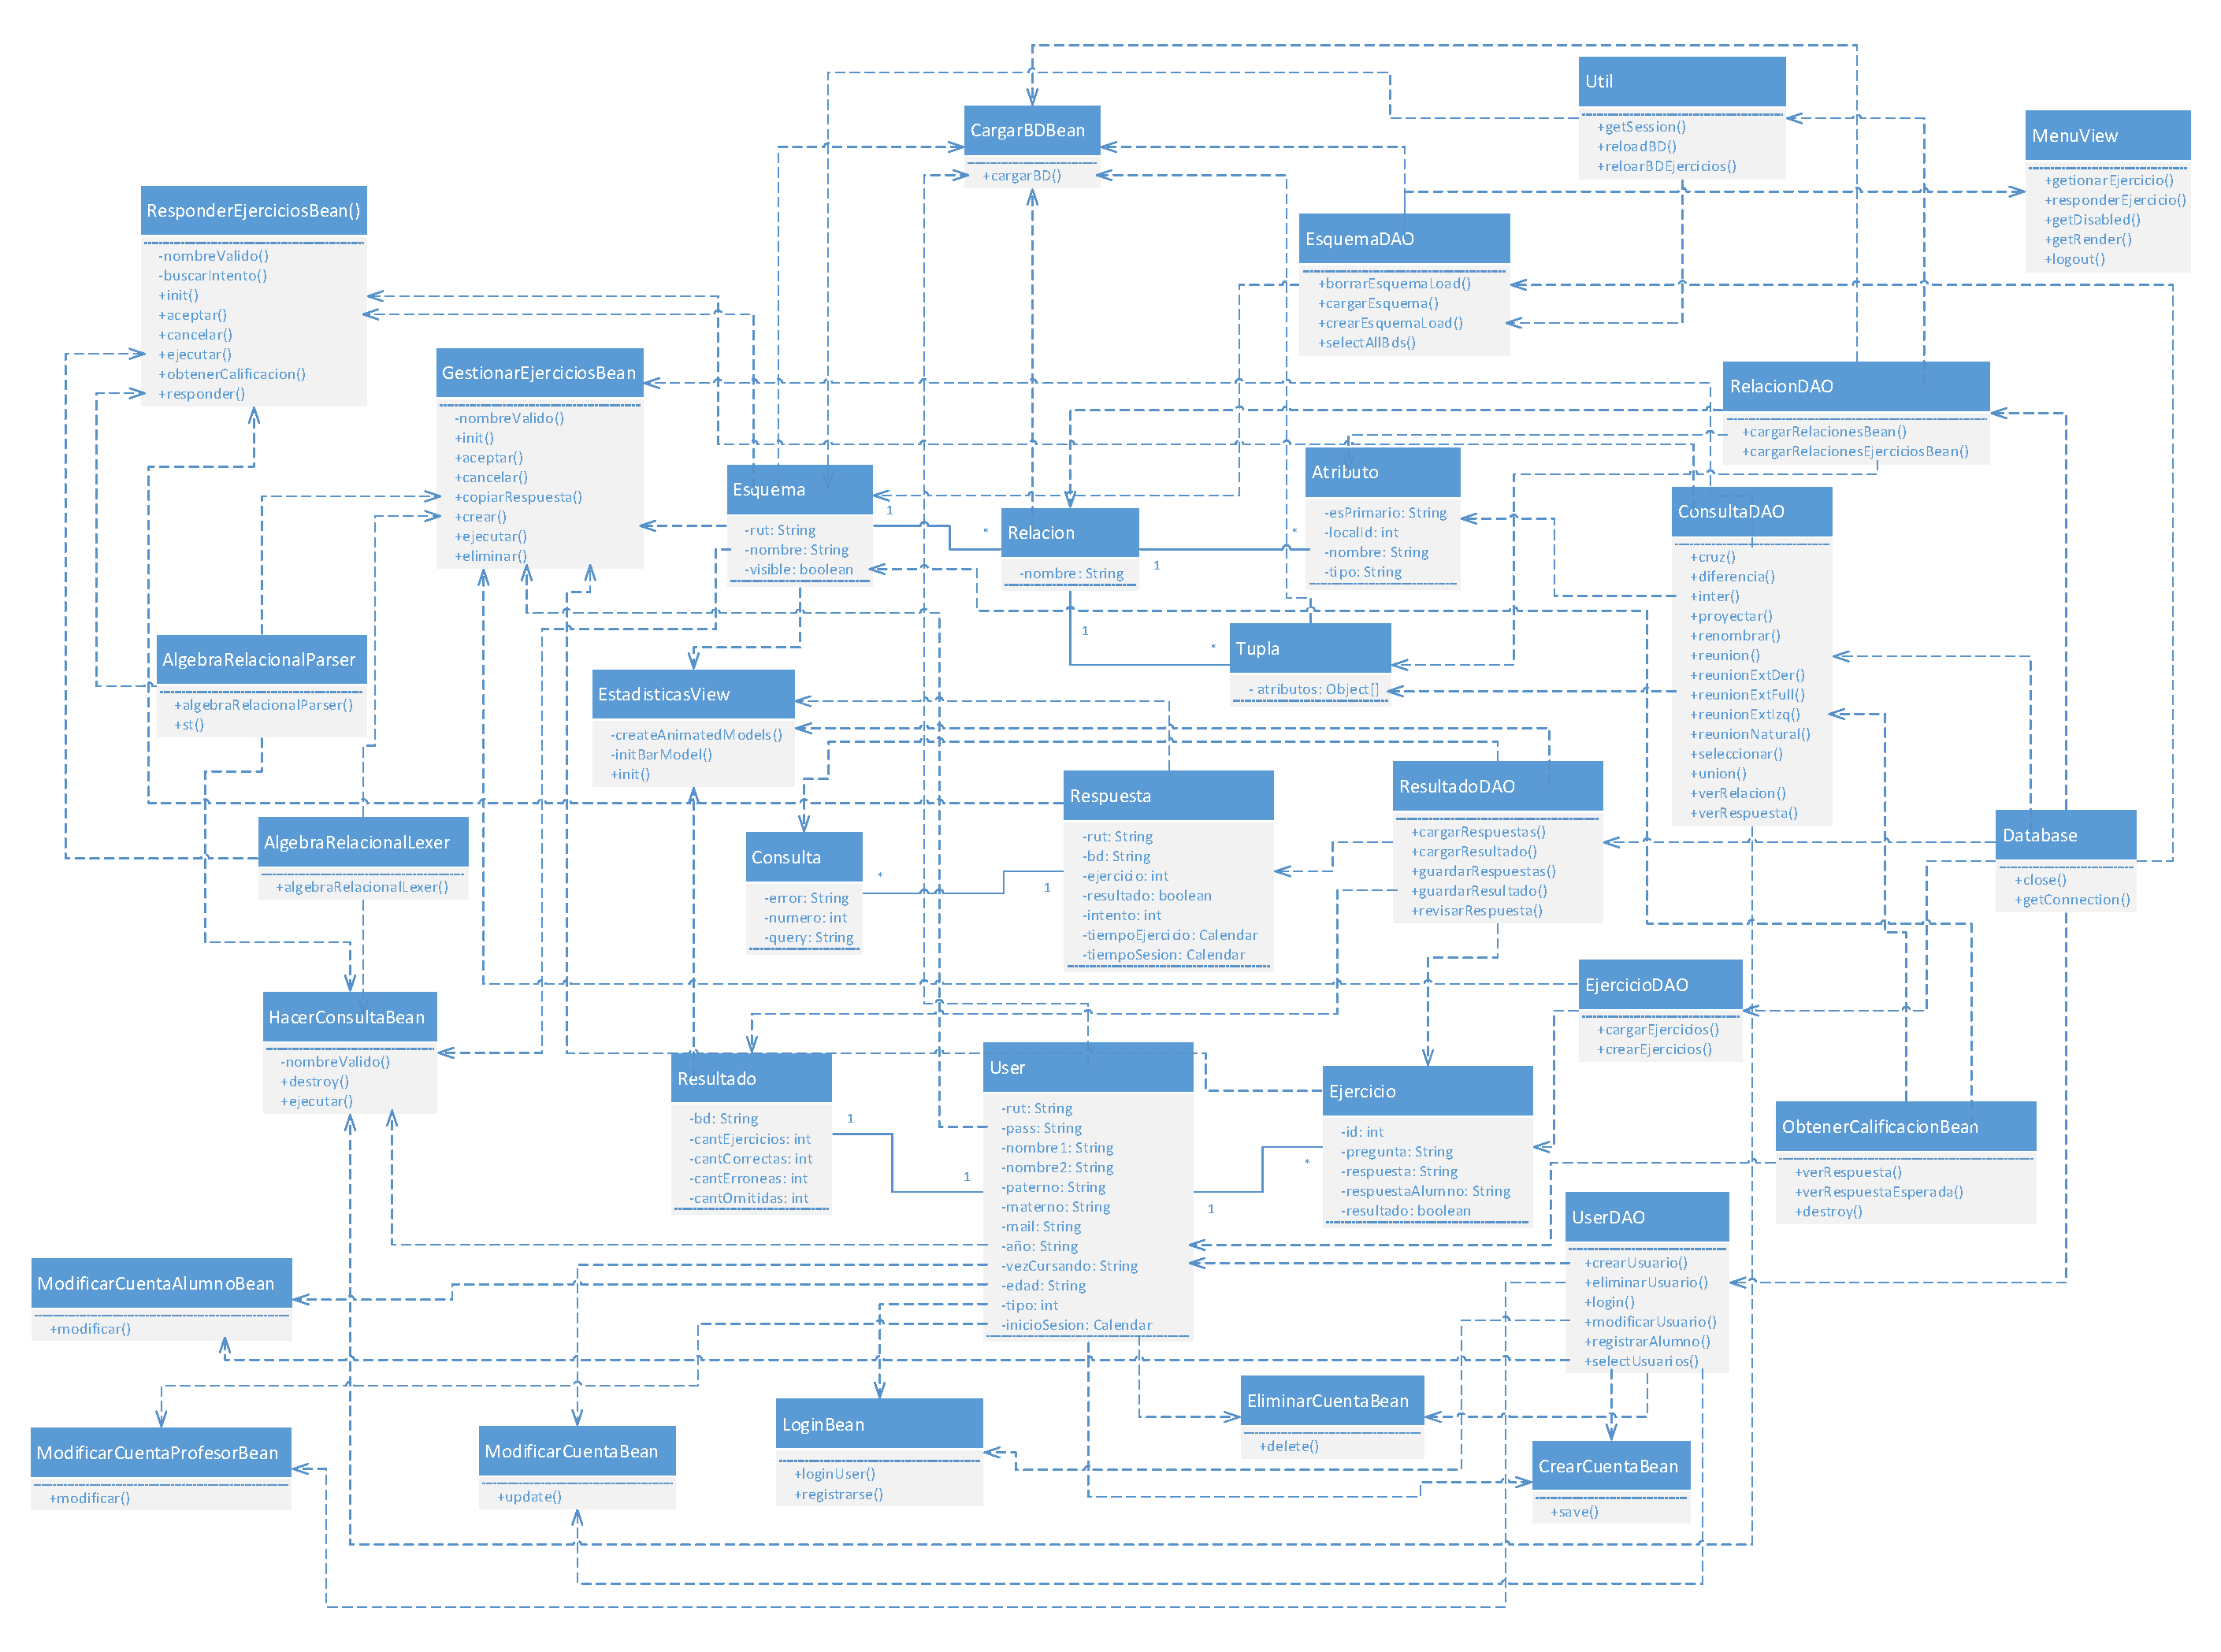
\includegraphics[width=21cm,angle=90]{imagenes/diagrama_clases.pdf}
\caption{Diagrama de Clases.}
\label{fig:diagramadeclases}
\end{figure}

%\subsection{Archivo de Registro}
%\label{archivoderegistro}

\newpage
\clearpage
\section{Dise�o de Datos}
\label{disenodedatos}

En la presente secci�n se muestra el dise�o del manejo de datos de la aplicaci�n a desarrollar. En la Secci�n \ref{modeloer} se explica el Modelo Entidad/Relaci�n, en la Secci�n \ref{modelodedatos} se muestra el Modelo interno de Datos y en la Secci�n \ref{diccionariodedatos} se muestra el Diccionario de Datos que explica en detalle el modelo presentado en la Secci�n \ref{modelodedatos} Modelo de Datos. \\

\subsection{Modelo Entidad/Relaci�n}
\label{modeloer}

En la Figura \ref{fig:modeloer} se presenta el Modelo Entidad/Relaci�n de la aplicaci�n a desarrollar. �sta muestra las distintas entidades y las relaciones que hay entre ellas. A continuaci�n se da una explicaci�n de cada entidad:

\begin{figure}[h!]
\centering
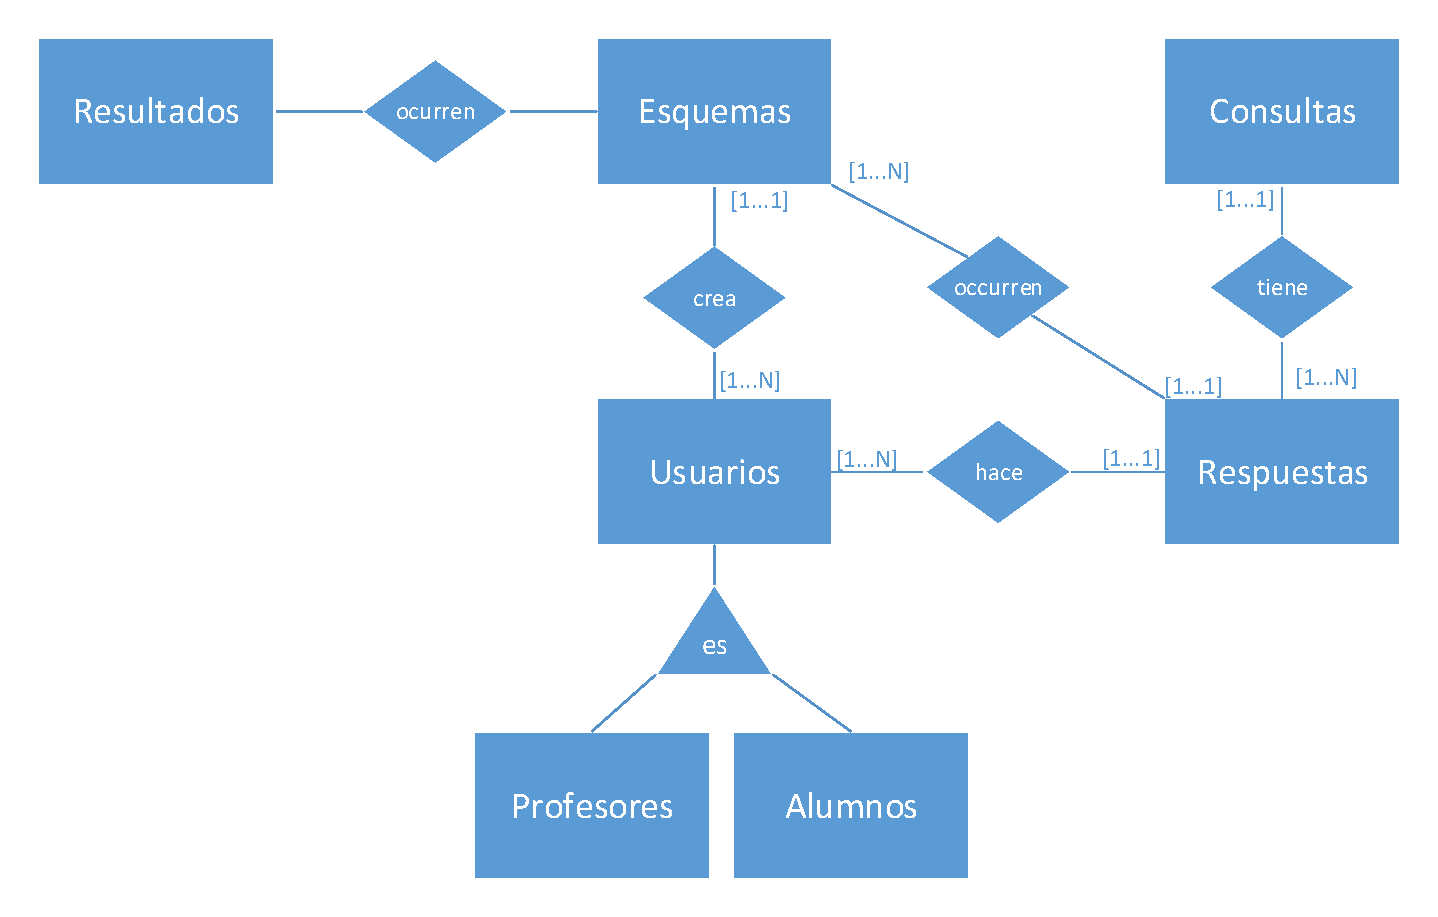
\includegraphics[width=14cm]{imagenes/modelo_er.pdf}
\caption{Modelo Entidad/Relaci�n.}
\label{fig:modeloer}
\end{figure}

\begin{itemize}

\item \textbf{Usuarios:} Entidad que refleja los usuarios que interact�an con el sistema, tanto profesores como alumnos.
\item \textbf{Profesores:} Entidad d�bil que depende de la existencia de la entidad \textit{Usuarios}. �sta indica el profesor que interact�a con el sistema.
\item \textbf{Alumnos:} Entidad d�bil que depende de la existencia de la entidad \textit{Usuarios}. �sta indica los alumnos que interact�an con el sistema.
\item \textbf{Esquemas:} Entidad que refleja las bases de datos que son creadas por los usuarios en el sistema.
\item \textbf{Resultados:} Entidad que guarda los resultados de los ejercicios que tiene cada base de datos.
\item \textbf{Respuestas:} Entidad que refleja las respuestas que se hacen al completar cualquier ejercicio.
\item \textbf{Consultas:} Entidad que refleja las consultas que se hacen al responder cualquier ejercicio.


\end{itemize}

\newpage
\subsection{Modelo de Datos}
\label{modelodedatos}

En la Figura \ref{fig:modelodedatos} se muestra el Modelo de Datos de la aplicaci�n a desarrollar. En �l, se aprecian las distintas entidades obtenidas en la Secci�n \ref{modeloer}. La Secci�n \ref{diccionariodedatos} explica en detalle cada entidad y c�mo se compone. \\

\begin{figure}[h!]
\centering
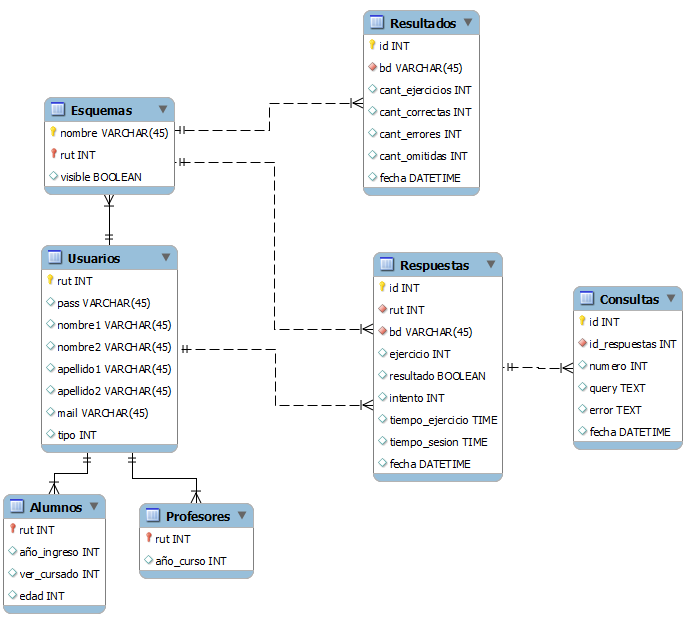
\includegraphics[width=14cm]{imagenes/modelo_datos.png}
\caption{Modelo de Datos.}
\label{fig:modelodedatos}
\end{figure}

\newpage
\subsection{Diccionario de Datos}
\label{diccionariodedatos}

En el Ap�ndice \ref{app-diccionariodedatos} se muestra en detalle el diccionario de datos que utilizar� el sistema. \\

\section{Dise�o de Pruebas}
\label{disenodepruebas}

En esta secci�n se muestra la elaboraci�n de distintas pruebas que tienen como objetivo principal la evaluaci�n de la calidad del sistema, asegurando que �ste cumpla con los requerimientos establecidos. En la Secci�n \ref{usuariosdepruebas} se definen los usuarios que participar�n en las pruebas, en la Secci�n \ref{pruebasunitarias} se definen las Pruebas Unitarias, despu�s en la Secci�n \ref{pruebasdeintegracion} se muestran las Pruebas de Integraci�n, en la Secci�n \ref{pruebasdesistemas} se explican las Pruebas de sistemas, despu�s en la Secci�n \ref{pruebasdeaceptacion} se definen las Pruebas de Aceptaci�n, luego en la Secci�n \ref{pruebasdeusabilidad} se muestran las Pruebas de Usabilidad, en la Secci�n \ref{pruebasdeestres} se definen las Pruebas de Estr�s y finalmente en la Secci�n \ref{pruebasdeseguridad} se describen las Pruebas de Seguridad. \\

\subsection{Usuarios de Pruebas}
\label{usuariosdepruebas}

Para la realizaci�n de las pruebas, ser� imperioso contar con la ayuda de diferentes usuarios agrupados en 4 asociaciones, quienes tendr�n como objetivo evaluar la funcionalidad del sistema. Estos usuarios est�n clasificados en funci�n a su nivel de conocimiento en Modelo de Datos y �lgebra Relacional. A continuaci�n se muestran los distintos grupos, especificando las distintas pruebas que tendr�n que ejecutar. \\

\begin{itemize}

\item \textbf{Grupo A:} En este grupo se encuentra el desarrollador del presente Trabajo de T�tulo, quien con conocimientos sobre el funcionamiento, estructura e interacci�n del sistema, ejecutar� las pruebas unitarias e integraci�n. \\

\item \textbf{Grupo B:} En este grupo se encuentra el profesor de la asignatura Modelo de Datos. Al ser el cliente del sistema y conocer a cabalidad los requerimientos funcionales y no funcionales, ser� el encargado de realizar las Pruebas de Sistema, adem�s de participar en las Pruebas de Aceptaci�n y Usabilidad. \\

\item \textbf{Grupo C:} En este grupo est� los alumnos de la Universidad de Valpara�so de la Escuela de Ingeniar�a Civil en Inform�tica que hayan aprobado la asignatura de Modelo de Datos y Sistema de Base de Datos. �sto debido a sus fuertes conocimientos en Modelo Relacional y �lgebra Relacional. Ellos participar�n en las Pruebas de Aceptaci�n y Usabilidad. \\

\item \textbf{Grupo D:} En este grupo se encuentran los alumnos de la Universidad de Valpara�so de la Escuela de Ingenier�a Civil Inform�tica que hayan aprobado la Asignatura de Modelo de Datos durante el primer semestre del a�o 2014, ya que ellos tienen un grado de conocimiento Medio en Modelo Relacional y �lgebra Relacional. Este grupo participar� de las Pruebas de Aceptaci�n y Usabilidad. \\

\end{itemize}

\subsection{Pruebas Unitarias}
\label{pruebasunitarias}

Las pruebas unitarias tienen como fin probar el correcto funcionamiento de las funciones del sistema, asegurando que cada procedimiento act�e de forma correcta. Estas pruebas ser�n efectuadas por el desarrollador al terminar la implementaci�n de cada funcionalidad mediante pruebas de Caja Negra. \\

Para ejecutar este tipo de pruebas, es necesario analizar las funcionalidades del sistemas, las cuales son extra�das de la Secci�n \ref{casosdeusosreales} Casos de Usos Reales, luego se define la entrada espec�fica y la salida esperada en funci�n de dicha entrada.  Si el resultado de la prueba no es el esperado, entonces se ha encontrado un error. Las Tablas \ref{tab:pruebasunitarias-1/3}, \ref{tab:pruebasunitarias-2/3} y \ref{tab:pruebasunitarias-3/3} muestran la definici�n de todos los casos de pruebas. Para aprobar la evaluaci�n, el comportamiento del sistema del 100\% de las pruebas realizadas, debe ser el esperado. En caso de que alguna funcionalidad no llegase a aprobar la evaluaci�n, �sta se debe re-codificar y ser testeada nuevamente hasta ser aprobada.  \\

\newpage
\clearpage
\begin{table}[h!]
\footnotesize
\centering
\begin{tabular}{|p{1.5cm}|p{1.5cm}|p{2cm}|p{4.5cm}|p{4.5cm}|}
\hline
\rowcolor[HTML]{C0C0C0} 
\textbf{Id Prueba Unitaria} & \textbf{Id Caso de Uso Real} & \textbf{Nombre Caso de Uso Real} & \textbf{Entrada}                                                                                                                                                                                                                                          & \textbf{Salida Esperada}                                                                    \\ \hline
PU01                        & CUR01                        & Crear Cuenta desde Inicio                    & Rellenar todos los campos pedidos para la creaci�n de una cuenta de tipo Alumno (ingresando desde el men� inicial), apretar el bot�n Siguiente y seguir ingresando los datos del nuevo Alumno, hasta apretar el bot�n Acepetar para crear la nueva cuenta & El sistema da aviso de la creaci�n de la cuenta y redirecciona al men� Inicio.              \\ \hline
PU02                        & CUR02                        & Iniciar Sesi�n                   & Ingresar datos de Username y Password v�lidos la cuenta de Profesor, luego seleccionar el bot�n Ingresar                                                                                                                                                  & El sistema carga la sesi�n del alumno ingresado y redirecciona al men� principal            \\ \hline
PU03                        & CUR07                        & Eliminar Cuenta                  & Seleccionar de la lista una cuenta a eliminar y confirmar la cuenta para eliminarla apretando el bot�n Aceptar                                                                                                                                            & El sistema da aviso de la eliminaci�n de la cuenta y redirecciona al men� principal         \\ \hline
PU04                        & CUR08                        & Modificar Cuenta                 & Seleccionar de la lista una cuenta a modificar, modificar el campo de Nombre de la cuenta, apretar el bot�n Siguiente y confirmar la modificaci�n apretando el bot�n Aceptar                                                                              & El sistema da aviso de la modificaci�n de la cuenta y redirecciona al men� principal        \\ \hline
PU05                        & CUR10                        & Crear BD                         & Ingresar los campos para la creaci�n de la BD, apretar Siguiente y apretar el bot�n Aceptar                                                                                                                                                               & El sistema da aviso de la base de datos creada y redirecciona al men� principal             \\ \hline
PU06                        & CUR11                        & Eliminar BD                      & Seleccionar de la lista la base de datos a eliminar y confirmar la eliminaci�n apretando el bot�n Aceptar                                                                                                                                                 & El sistema da aviso de la eliminaci�n de la base de datos y redirecciona al men� principal  \\ \hline
PU07                        & CUR12                        & ModificarBD                      & Seleccionar de la lista la base de datos a modificar, modificar el campo de Nombre de la base de datos, apretar el bot�n Siguiente y confirmar la modificaci�n apretando el bot�n Aceptar                                                                 & El sistema da aviso de la modificaci�n de la base de datos y redirecciona al men� principal \\ \hline
PU08                        & CUR13                        & CargarBD                         & Seleccionar de la lista la base de datos a cargar y apretar el bot�n Aceptar                                                                                                                                                                              & El sistema da aviso de la carga de la base de datos y redirecciona al men� principal        \\ \hline
PU09                        & CUR15                        & Gesti�n Ejercicios              & Seleccionar de la lista un ejercicio a eliminar y confirmar la eliminaci�n & El sistema guarda los cambios y da aviso al usuario \\ \hline
\end{tabular}
\caption{Pruebas Unitarias (1/3).}
\label{tab:pruebasunitarias-1/3}
\end{table}

\newpage
\clearpage
\begin{table}[h!]
\footnotesize
\centering
\begin{tabular}{|p{1.5cm}|p{1.5cm}|p{2cm}|p{4.5cm}|p{4.5cm}|}
\hline
\rowcolor[HTML]{C0C0C0} 
\textbf{Id Prueba Unitaria} & \textbf{Id Caso de Uso Real} & \textbf{Nombre Caso de Uso Real} & \textbf{Entrada}                                                                                                                                                                                              & \textbf{Salida Esperada}                                                                                                                                                                         \\ \hline
PU10                        & CUR15                        & Gesti�n Ejercicios              & Seleccionar de la lista un ejercicio a modificar, modificar los campos del ejercicio y confirmar la modificaci�n & El sistema guarda los cambios y da aviso al usuario \\ \hline
PU11                        & CUR15                        & Gesti�n Ejercicios              & Agregar un nuevo ejercicio y confirmar la acci�n & El sistema guarda los cambios y da aviso al usuario \\ \hline
PU12                        & CUR16                        & Responder Ejercicios             & Para cada ejercicio hacer una serie de consultas, luego apretar el bot�n Responder, apretar el bot�n Siguiente para pasar a la siguiente pregunta hasta responderlas todas                                    & El sistema muestra una lista de los ejercicios correctos e incorrectos y el porcentaje de acetadas en funci�n de las respustas dadas. El sistema entrega la opci�n para volver al men� principal \\ \hline
PU13                        & CUR18                        & Agregar Relaci�n                 & Agregar los campos necesarios para la creaci�n de la relaci�n, apretar Siguiente y apretar el bot�n Aceptar                                                                                                   & El sistema da aviso da la nueva relaci�n y redirecciona al men� principal                                                                                                                        \\ \hline
PU14                        & CUR29                        & Eliminar Relaci�n                & Seleccionar de la lista la relaci�n a eliminar y confirmar la eliminaci�n apretando el bot�n Aceptar                                                                                                          & El sistema da aviso de la eliminaci�n de la relaci�n y redirecciona al men� principal                                                                                                            \\ \hline
PU15                        & CUR20                        & Modificar Relaci�n               & Seleccionar de la lista la relaci�n a modificar, modificar el campo nombre de la relaci�n, apretar el bot�n Siguiente y confirmar la modificaci�n apretando el bot�n Aceptar                                  & El sistema da aviso de la modificaci�n de la relaci�n y redirecciona al men� principal                                                                                                           \\ \hline
PU16                        & CUR21                        & Ver Relaci�n                     & Seleccionar de la lisa la relaci�n a ver y apretar el bot�n Siguiente                                                                                                                                         & El sistema muestra por pantalla la relaci�n seleccionada y el men� gestionar tupla                                                                                                               \\ \hline
PU17                        & CUR23                        & Ingresar Tupla                   & Agregar los campos necesarios para la creaci�n de la tupla y apretar el bot�n Aceptar                                                                                                             & El sistema da aviso de la nueva tupla y redirecciona al men� gestionar tupla              \\ \hline
PU18                        & CUR24                        & Eliminar Tupla                   & Seleccionar de la lista la tupla a eliminar y confirmar la eliminaci�n apretando el bot�n Aceptar                                                                                                 & El sistema da aviso de la eliminaci�n de la tupla y redirecciona al men� gestionar tupla  \\ \hline
PU19                        & CUR25                        & Modificar Tupla                  & Seleccionar de la lista la tupla a modificar, modificar alg�n campo de la tupla (exceptuando la clave primaria), apretar el bot�n Siguiente y confirmar la eliminaci�n apretando el bot�n Aceptar & El sistema da aviso de la modificaci�n de la tupla y redirecciona al men� gestionar tupla \\ \hline
\end{tabular}
\caption{Pruebas Unitarias (2/3).}
\label{tab:pruebasunitarias-2/3}
\end{table}

\newpage
\clearpage
\begin{table}[h!]
\footnotesize
\centering
\begin{tabular}{|p{1.5cm}|p{1.5cm}|p{2cm}|p{4.5cm}|p{4.5cm}|}
\hline
\rowcolor[HTML]{C0C0C0} 
\textbf{Id Prueba Unitaria} & \textbf{Id Caso de Uso Real} & \textbf{Nombre Caso de Uso Real} & \textbf{Entrada}                                                                                                                                                                                  & \textbf{Salida Esperada}                                                                  \\ \hline
PU20                        & CUR27                        & Hacer Consulta                   & Ingresar una consulta v�lida en una base de datos ya seleccionada y apretar el bot�n Ejecutar                                                                                                     & El sistema muestra por pantalla el resultado de la consulta                               \\ \hline
PU21                        & CUR29                        & Ver Estad�sticas                 & Seleccionar de la lista la base de datos a ver las estad�sticas, apretar el bot�n Siguiente & El sistema muestra por pantalla las estad�sticas b�sicas y permite al usuario descargar Reglas de Asociaci�n o Gr�ficos detallados                              \\ \hline
\end{tabular}
\caption{Pruebas Unitarias (3/3).}
\label{tab:pruebasunitarias-3/3}
\end{table}

Para la verificaci�n de los datos de prueba, se debe completar la plantilla de registro de informaci�n que se presenta en la Tabla \ref{tab:plantilapruebasunitarias}. �sta debe ser llenada con la informaci�n de la Prueba Unitaria, observaciones del comportamiento del sistema para cada testeo y el resultado indicando si es aceptado o no.\\

\begin{table}[h!]
\footnotesize
\centering
\begin{tabular}{|p{3.5cm}|p{9cm}|p{2cm}|}
\hline
\rowcolor[HTML]{9B9B9B} 
\multicolumn{2}{|p{12.5cm}|}{\cellcolor[HTML]{9B9B9B}\textbf{Prueba Unitaria}} & \textbf{Id:} \\ \hline
Nombre                                      & \multicolumn{2}{l|}{}                   \\ \hline
Referencias                                 & \multicolumn{2}{l|}{}                   \\ \hline
\rowcolor[HTML]{C0C0C0} 
\multicolumn{3}{|l|}{\cellcolor[HTML]{C0C0C0}\textit{Caso de Prueba}}                 \\ \hline
Entrada V�lida                              & \multicolumn{2}{l|}{}                   \\ \hline
Salida Esperada                             & \multicolumn{2}{l|}{}                   \\ \hline
Entrada Inv�lida                            & \multicolumn{2}{l|}{}                   \\ \hline
Salida Esperada                             & \multicolumn{2}{l|}{}                   \\ \hline
Entrada Vac�a                               & \multicolumn{2}{l|}{}                   \\ \hline
Saluda Esperada                             & \multicolumn{2}{l|}{}                   \\ \hline
\textbf{Resultado}                          & \multicolumn{2}{l|}{}                   \\ \hline
\end{tabular}
\caption{Plantilla Pruebas Unitarias.}
\label{tab:plantilapruebasunitarias}
\end{table}

%\begin{table}[h!]
%\footnotesize
%\centering
%\begin{tabular}{|p{4cm}|p{10.5cm}|}
%\hline
%\multicolumn{2}{|c|}{\cellcolor[HTML]{9B9B9B}\textbf{Nombre Caso de Pruebas}} \\ \hline
%Prop�sito                                      &                              \\ \hline
%Referencias                                    &                              \\ \hline
%\multicolumn{2}{|c|}{\cellcolor[HTML]{C0C0C0}\textit{Caso de Prueba}}         \\ \hline
%Entrada V�lida                                 &                              \\ \hline
%Salida Esperada                                &                              \\ \hline
%Entrada Inv�lida                               &                              \\ \hline
%Salida Esperada                                &                              \\ \hline
%Entrada Vac�a                                  &                              \\ \hline
%Saluda Esperada                                &                              \\ \hline
%\textbf{Resultado}                             &                              \\ \hline
%\end{tabular}
%\caption{Plantilla Pruebas Unitarias}
%\label{tab:plantilapruebasunitarias}
%\end{table}

\subsection{Pruebas de Integraci�n}
\label{pruebasdeintegracion}

Para revisar el correcto ensamblaje y funcionamiento entre los distintos componentes del sistema una vez que hayan sido probados como unidad, se realizar�n pruebas de integraci�n. �stas corresponden a evaluaciones que permiten encontrar errores entre la interacci�n de los componentes. \\

La realizaci�n de estas pruebas ser�n siguiendo la t�cnica de Pruebas de Caja Negra y estar�n regidas por una estrategia incremental, es decir, cada vez que se implemente un m�dulo y sea integrado, el sistema ser� probado en su totalidad. De esta forma, se sigue paralelamente la estrategia de desarrollo. Adem�s, para aprobar el testing, el 100\% de las pruebas deben tener resultados favorables, es decir, que cada salida sea la esperada. Si alguna prueba sale rechazada, �sta debe ser re-codificada y testeada nuevamente hasta que sea aprobada. \\

\begin{figure}[h!]
\centering
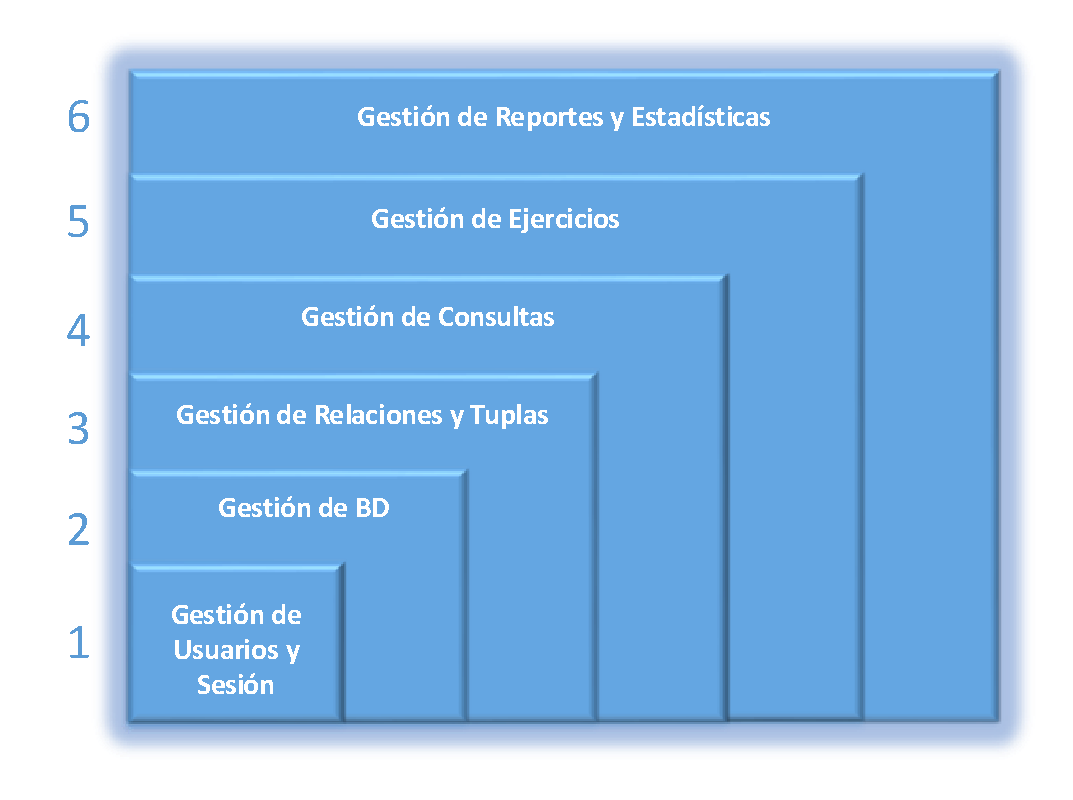
\includegraphics[width=10cm]{imagenes/pruebas_integracion.pdf}
\caption{Pruebas de Integraci�n.}
\label{fig:pruebasdeintegracion}
\end{figure}

\begin{table}[h!]
\footnotesize
\centering
\begin{tabular}{|p{3.5cm}|p{9cm}|p{2cm}|}
\hline
\rowcolor[HTML]{9B9B9B} 
\multicolumn{2}{|p{12.5cm}|}{\cellcolor[HTML]{9B9B9B}\textbf{Prueba de Integraci�n}} & \textbf{Id:} \\ \hline
Nombre                                         & \multicolumn{2}{l|}{}                      \\ \hline
Componentes                                    & \multicolumn{2}{l|}{}                      \\ \hline
Objetivo                                       & \multicolumn{2}{l|}{}                      \\ \hline
\rowcolor[HTML]{C0C0C0} 
\multicolumn{3}{|l|}{\cellcolor[HTML]{C0C0C0}\textit{Caso de Prueba}}                       \\ \hline
Estado Inicial                                 & \multicolumn{2}{l|}{}                      \\ \hline
Estado Final                                   & \multicolumn{2}{l|}{}                      \\ \hline
Procedimiento                                  & \multicolumn{2}{l|}{}                      \\ \hline
Resultado Esperado                             & \multicolumn{2}{l|}{}                      \\ \hline
\textbf{Resultado}                             & \multicolumn{2}{l|}{}                      \\ \hline
\end{tabular}
\caption{Plantilla Pruebas de Integraci�n.}
\label{tab:pruebasdeintegracion}
\end{table}


La Figura \ref{fig:pruebasdeintegracion} muestra gr�ficamente la implementaci�n de las pruebas de integraci�n, partiendo desde las pruebas de los m�dulos de Gesti�n de Usuarios y Cuentas, para finalizar con el m�dulo de Gesti�n de Reportes y Estad�sticas. Cada prueba debe ser ejecutada y registrada en el formulario que se muestra en la Tabla \ref{tab:pruebasdeintegracion} tal como se explico en la Secci�n \ref{pruebasunitarias} Pruebas Unitarias. \\

\subsection{Pruebas de Sistema}
\label{pruebasdesistemas}

El grupo que participa en las Pruebas de Sistema se indica en la Secci�n \ref{usuariosdepruebas}. La idea de este tipo de pruebas es revisar el sistema como un todo, englobando todos los requerimientos presentados en el Capitulo \ref{analisis} de An�lisis, en la Secci�n \ref{espreq} de Especificaci�n de Requerimientos. Por ende, se considera que cada requerimiento ser� evaluado con una nota que estar� en funci�n de los siguientes par�metros: \\

\begin{itemize}

\item \textbf{Completo (C):} El requerimiento est� desarrollado en su totalidad y cumple con lo esperado.
\item \textbf{Completo con Modificaciones (CM):} El requerimiento est� desarrollado, pero con modificaciones.
\item \textbf{No Completo (NC):} El requerimiento no est� desarrollado. \\

\end{itemize}

Finalmente es el profesor de Modelo de Datos quien est� encargado de la implementaci�n de las pruebas de sistema. Para �sto, el profesor debe rellenar con una $\emph{X}$ en la Tabla \ref{tab:prueebasdesistema} para especificar la calificaci�n de cada requerimiento. Para aprobar el testing, el 30\% o menos de los requerimientos obligatorios  y deseables deben estar marcado como \textit{Completo con Modificaciones} y el 70\% o m�s como \textit{Completos}, los requerimientos prescindibles pueden estar marcados como \textit{No Completo}. Si el testing sale rechazado, se deber� volver a programar para volver a ser testeado hasta que �ste salga aprobado. \\

\begin{table}[h!]
\footnotesize
\centering
\begin{tabular}{|p{0.5cm}|p{10cm}|p{0.5cm}|p{0.5cm}|p{0.5cm}|}
\hline
\rowcolor[HTML]{9B9B9B} 
\multicolumn{2}{|l|}{\cellcolor[HTML]{9B9B9B}\textbf{Pruebas de Sistema}} & \multicolumn{3}{l|}{\cellcolor[HTML]{9B9B9B}\textbf{Id:}} \\ \hline
\rowcolor[HTML]{C0C0C0} 
\textit{Id}         & \textit{Requerimiento}         & \textit{C}         & \textit{CM}                 & \textit{NC}                 \\ \hline
                    &                                &                    &                             &                             \\ \hline
                    &                                &                    &                             &                             \\ \hline
                    &                                &                    &                             &                             \\ \hline
                    &                                &                    &                             &                             \\ \hline
                    &                                &                    &                             &                             \\ \hline
                    &                                &                    &                             &                             \\ \hline
\multicolumn{2}{|l|}{\textbf{Resultados}}            &                    &                             &                             \\ \hline
\end{tabular}
\caption{Plantilla Pruebas de Sistema.}
\label{tab:prueebasdesistema}
\end{table}

\subsection{Pruebas de Aceptaci�n}
\label{pruebasdeaceptacion}

Para llevar a cabo las pruebas de aceptaci�n, los usuarios de Grupos C y D definidos en la Secci�n \ref{usuariosdepruebas} deben realizar una serie de tareas. Los usuarios del Grupo C deben ejecutar las tareas que se muestran en la Tabla \ref{tab:tareasperfilprofesor} correspondiente al perfil de profesor y los usuarios del Grupo D deben ejecutar las tareas de la Tabla \ref{tab:tareasperfilusuario} correspondiente a las tareas del perfil de alumno. \\

\begin{table}[h!]
\footnotesize
\centering
\begin{tabular}{|p{7.5cm}|p{3.5cm}|p{2cm}|}
\hline
\rowcolor[HTML]{9B9B9B} 
\multicolumn{2}{|l|}{\cellcolor[HTML]{9B9B9B}\textbf{Tareas Perfil Alumno}}                                                                                                                                                                                                                 & \textbf{Id:}              \\ \hline
\rowcolor[HTML]{C0C0C0}  
\textit{Tarea}                                                                                                                                                                                                               & \textit{Funci�n(es)}                           & \textit{Tiempo Requerido} \\ \hline
1) Usted desea ingresar al sistema como alumno, pero no tiene cuenta. Para ello, cree su propia cuenta e ingrese al Sistema                                                                                                  & Crear Cuenta, Iniciar Sesi�n, Modificar Cuenta & 5 minutos                 \\ \hline
2) Usted desea crear una nueva base de datos llamada "univ"                                                                                                                                                                  & Crear BD                                       & 2 minutos                 \\ \hline
3) Usted desea modificar la base de datos "univ" y llamarla "universidad"                                                                                                                                                    & Modificar BD                                   & 2 minutos                 \\ \hline
4) Usted desea cargar la base de datos "universidad"                                                                                                                                                                         & Cargar BD                                      & 1 minuto                  \\ \hline
5) Usted desea crear una relaci�n llamada "alumnos" con 3 atributos: un atributo de tipo "Entero" llamado "id" de tipo primario y 2 atributos de tipo "Cadena" llamados "nombre" y "apellido"                                & Crear Relaci�n                                 & 5 minutos                 \\ \hline
6) Usted desea modificar la relaci�n "alumnos" y renombrarla como "personas"                                                                                                                                                 & Modificar Relaci�n                             & 2 minutos                 \\ \hline
7) Usted desea agregar 3 tuplas a la relaci�n "personas": uno con id=1, nombre="nombre1", apellido="apellido1"; otro con id=2, nombre="nombre2", apellido="apellido2" y otro con id=3, nombre="nombre3", apellido="apellido3" & Crear Tupla                                    & 5 minutos                 \\ \hline
8) Usted desea hacer una consulta de tipo "proyectar" que retorne todos los nombres de la relaci�n "personas". Para ello usted debe hacer la consulta "proyectar(nombre)(personas)"                                                                                                                 & Hacer Consulta                                 & 5 minutos                 \\ \hline
9) Usted desea eliminar la relaci�n "personas"                                                                                                                                                                                & Eliminar Relaci�n                              & 2 minutos                 \\ \hline
10) Usted desea eliminar la base de datos "universidad"                                                                                                                                                                      & Eliminar BD                                    & 2 minutos                 \\ \hline
11) Usted desea cargar la base de datos "ejemplo" y responder los ejercicios de esta base de datos                                                                                                                           & Responder Ejercicios                           & 10 minutos                \\ \hline
\end{tabular}
\caption{Tareas Perfil Alumno}
\label{tab:tareasperfilusuario}
\end{table}

\begin{table}[h!]
\footnotesize
\centering
\begin{tabular}{|p{7.5cm}|p{3.5cm}|p{2cm}|}
\hline
\rowcolor[HTML]{9B9B9B} 
\multicolumn{2}{|l|}{\cellcolor[HTML]{9B9B9B}\textbf{Tareas Perfil Profesor}}                                                                                                                                                                                                                 & \textbf{Id:}              \\ \hline
\rowcolor[HTML]{C0C0C0} 
\textit{Tarea}                                                                                                                                                                                                                                                         & \textit{Funci�n(es)} & \textit{Tiempo Requerido} \\ \hline
1) Usted desea ingresar al sistema como profesor, ingrese al sistema como rut="12345678" y contrase�a="admin"                                                                                                                                                          & Iniciar Sesi�n       & 1 minuto                  \\ \hline
2) Usted desea ingresar un nuevo alumno al sistema. Para ello, utilize sus propios datos como el nuevo alumno a agregar                                                                                                                                                & Crear Cuenta         & 5 minutos                 \\ \hline
3) Usted desea modificar al nuevo alumno ingresado y desea cambiar su mail por "usuario@mail.com"                                                                                                                                                                      & Modificar Cuenta     & 2 minutos                 \\ \hline
4) Usted desea eliminar al nuevo alumno                                                                                                                                                                                                                                & Eliminar Cuenta      & 1 minuto                  \\ \hline
5) Usted desea cargar la base de datos "ejemplos" y generar un nuevo ejercicio. Para ello usted deber� crear el ejercicio como pregunta="Mostrar todos los datos de los trabajadores que son de administraci�n y producci�n". Adem�s, deber� ejecutar la consulta="resp := empleados\_adm inter empleados\_prod" y agregar la relaci�n generada "resp" en el campo Nombre Relaci�n Resultante. En consultas, deber� agregar la consulta ingresada para generar la relaci�n resultante. Finalmente Acepta y Guarda los Cambios. & Agregar Ejercicio    & 10 minutos                 \\ \hline
6) Usted desea ver las estad�sticas de la base de datos "ejemplo\_17134298" con fecha "2014-10-01". & Ver Estad�sticas & 2 minutos \\ \hline
\end{tabular}
\caption{Tareas Perfil Profesor}
\label{tab:tareasperfilprofesor}
\end{table}

Posteriormente, los sujetos de pruebas deber�n responder el formulario de aceptaci�n que se muestra en la Tabla \ref{tab:formulariodeaceptacion}, el cual contiene preguntas enfocadas a c�mo el usuario percibi� la experiencia. Este formulario ser� respondido en funci�n de los par�metros de evaluaci�n que se muestran en la Tabla \ref{tab:listadeparametros}.

\clearpage
\begin{table}[h!]
\footnotesize
\centering
\begin{tabular}{|l|l|l|}
\hline
\rowcolor[HTML]{9B9B9B} 
\multicolumn{3}{|c|}{\cellcolor[HTML]{9B9B9B}\textbf{Par�metros de Evaluaci�n}}           \\ \hline
\rowcolor[HTML]{C0C0C0} 
\textit{Par�metro} & \textit{Asignaci�n} & \textit{Descripci�n}                           \\ \hline
0                  & Malo                & Tarea con mal funcionamiento                   \\ \hline
1                  & Deficiente          & Tarea con funcionamiento incompleto            \\ \hline
2                  & Regular             & Tarea realizada con �xito, pero poco efectiva  \\ \hline
3                  & Satisfecho          & Tarea realizada de manera efectiva             \\ \hline
4                  & �ptimo              & Tarea realizada de manera eficiente y efectiva \\ \hline
\end{tabular}
\caption{Par�metros de Evaluaci�n.}
\label{tab:listadeparametros}
\end{table}

\begin{table}[h!]
\footnotesize
\centering
\begin{tabular}{|p{10cm}|p{3cm}|}
\hline
\rowcolor[HTML]{9B9B9B} 
\textbf{Prueba de Aceptaci�n}                                                                       & \textbf{Id:}        \\ \hline
\rowcolor[HTML]{C0C0C0} 
\textit{Preguntas}                                                                                  & \textit{Evaluaci�n [0 - 4]} \\ \hline
\textbf{Funcionamiento del Sistema}                                                                 &                     \\ \hline
1) �El sistema funciona eficazmente?                                                                &                     \\ \hline
2) �El sistema arroja los resultados que esperaba?                                                 &                     \\ \hline
3) �La informaci�n entregada por el sistema es la adecuada?                                        &                     \\ \hline
4) �Recibe retroalimentaci�n durante la ejecuci�n de alguna funcionalidad del sistema?             &                     \\ \hline
5) �Consider� el sistema amigable para su funcionamiento?                                          &                     \\ \hline
6) �Consider� que el tiempo que demor� la b�squeda es el apropiado?                                &                     \\ \hline
7) �La retroalimentaci�n entregada por el sistema le resulto �til?                                 &                     \\ \hline
8) �C�mo eval�a usted el funcionamiento del sistema?                                               &                     \\ \hline
\end{tabular}
\caption{Formulario de Aceptaci�n.}
\label{tab:formulariodeaceptacion}
\end{table}

Para validar completamente las pruebas de aceptaci�n, las respuestas de cada pregunta de la Tabla \ref{tab:formulariodeaceptacion} deben estar valorizadas con par�metro 3 o superior. Si no aprueba, se deber� volver a implementar para ser testeado nuevamente hasta aprobar el testing. \\

\subsection{Pruebas de Usabilidad}
\label{pruebasdeusabilidad}

Luego de ejecutar las Pruebas de Aceptaci�n presentadas en la Secci�n \ref{pruebasdeaceptacion}, los sujetos de pruebas deber�n ejecutar las Pruebas de Usabilidad, respondiendo el formulario de usabilidad que se presenta en la Tabla \ref{tab:formulariodeusabilidad}. \\

\begin{table}[h!]
\footnotesize
\centering
\begin{tabular}{|p{3cm}|p{1.5cm}|p{0.05cm}|p{1.5cm}|p{0.05cm}|p{1.5cm}|p{0.05cm}|p{1.5cm}|p{0.05cm}|p{1.5cm}|p{0.05cm}|}
\hline
\rowcolor[HTML]{9B9B9B} 
\multicolumn{9}{|l|}{\cellcolor[HTML]{9B9B9B}\textbf{Formulario de Usabilidad}}                                                                                          & \multicolumn{2}{l|}{\cellcolor[HTML]{9B9B9B}\textbf{Id:}} \\ \hline
\rowcolor[HTML]{C0C0C0} 
\textit{Preguntas}                                                                             & \multicolumn{10}{l|}{\cellcolor[HTML]{C0C0C0}\textit{Evaluaci�n (Marque con una X a la derecha de la casilla)}}                               \\ \hline
1) �C�mo encuentra la estructura de men�s y organizaci�n de las funciones del sistema?         & Muy Mala    &  & Mala      &  & Regular           &  & Buena         &  & Muy Buena                         &                       \\ \hline
2) �Los �conos del sistema son representativos respecto a las funcionalidades que representan? & Muy Malos   &  & Malos     &  & Regulares         &  & Buenos        &  & Muy Buenos                        &                       \\ \hline
3) �Encontr� f�cil la navegaci�n del sistema y obtener la informaci�n deseada?                 & Muy Dif�cil &  & Dif�cil   &  & Regular           &  & F�cil         &  & Muy F�cil                         &                       \\ \hline
4) �De qu� forma el sistema permite realizar las tareas solicitadas?                           & Muy Confusa &  & Confusa   &  & Levemente Confusa &  & Clara         &  & Muy Clara                         &                       \\ \hline
5) En general �Fue f�cil realizar las tareas solicitadas?                                      & Muy Dif�cil &  & Dif�cil   &  & Regular           &  & F�cil         &  & Muy F�cil                         &                       \\ \hline
6) �Usted cree que necesitar� ayuda para utilizar el sistema?                                  & Mucha Ayuda &  & Con Ayuda &  & Poca Ayuda          &  & Muy Poca Ayuda &  & Para Nada                         &                       \\ \hline
7) �Usted piensa que aprender� r�pidamente a usar el sistema?                                  & Muy Dif�cil &  & Dif�cil   &  & Tal Vez           &  & Casi Seguro   &  & Por Supuesto                      &                       \\ \hline
Sugerencias                                                                                    & \multicolumn{10}{l|}{}                                                                                                              \\ \hline
\end{tabular}
\caption{Formulario de Usabilidad.}
\label{tab:formulariodeusabilidad}
\end{table}

Para validar completamente las pruebas de usabilidad, el 100\% de las respuestas de la Tabla \ref{tab:formulariodeusabilidad} deben estar valorizadas con par�metro 2 o superior. Sino, se deber� programar la interfaz nuevamente y volver a ser testeado hasta aprobar el testing.

\newpage
\clearpage

\subsection{Pruebas de Estr�s}
\label{pruebasdeestres}

Las pruebas de estr�s tienen como objetivo verificar la disponibilidad del sistema al momento que muchos usuarios lo est�n usando paralelamente. Para ello se simular� una solicitud concurrente a la funcionalidad m�s utilizada del sistema, que en este caso es "Hacer consultas en �lgebra Relacional", y se verificar� la disponibilidad del sistema con una cantidad de usuarios determinados, que para esta prueba son 50 usuarios, los cuales representan la cantidad m�xima de alumnos que podr�an utilizar el sistema concurrentemente. \\

Para aprobar esta prueba, el sistema debe soportar por lo menos 50 usuarios concurrentes, sino se deber� recodificar el sistema y volver a ser testeado hasta aprobar las pruebas de estr�s. \\ 

\subsection{Pruebas de Seguridad}
\label{pruebasdeseguridad}

Las pruebas de seguridad tienen como fin garantizar que la aplicaci�n no presente errores respecto a la seguridad del mismo. Los temas a considerar en estas pruebas son: \\

\begin{itemize}

\item \textbf{SQL Injection:} se agregar�n comandos b�sicos de acceso a la base de datos. La idea es vulnerar la base de datos mediante comandos SQL. Los par�metros a evaluar sera la \textit{Presentaci�n de Informaci�n Relevante}, en otras palabras, si sistema accede o no a las peticiones SQL. Para pasar esta prueba, el sistema debe evitar en un 100\% la presentaci�n de informaci�n relevante de la base de datos. \\

\item \textbf{Acceso por URL:} se tratar� de acceder a los directorios de la aplicaci�n mediante URL. La idea es evitar que un usuario de tipo Alumno ingrese a una funcionalidad de un usuario de tipo Profesor. Para aprobar el Testing, el sistema debe denegar en un 100\% el ingreso de funcionalidades especiales de un usuario Profesor a un usuario Alumno.

\end{itemize}


\chapter{Implementaci�n}
\label{implementacion}

\section{Herramientas de Desarrollo}
\label{herramientasDeDesarrollo}

En esta secci�n se describen las herramientas orientadas al desarrollo del sistema. �stas cubren tanto el hardware utilizado, como los distintos softwares orientados a la codificaci�n, almacenamiento de datos y dise�o. \\

\subsection{Hardware de Desarrollo}
\label{hardwareDeDesarrollo}

Para el desarrollo de la aplicaci�n y la ejecuci�n de los distintos softwares de codificaci�n, almacenamiento de datos y dise�o, se utiliz� un computador personal con una serie de caracter�sticas. \\

\begin{itemize}

\item \textbf{Procesador}: Intel Core 2 Duo Mobile T6400 / 2.00 GHz. \\
\item \textbf{Memoria Ram}: 3 GB. \\
\item \textbf{Disco Duro}: 320 GB. \\
\item \textbf{Sistema Operativo}: Windows 7 Ultimate. \\

\end{itemize}

\subsection{Lenguajes de Programaci�n}
\label{lenguajesDeProgramacion}

Para la codificaci�n del sistema, se utilizaron dos lenguajes de programaci�n orientados a distintos subsistemas de la aplicaci�n:

\begin{itemize}

\item \textbf{Java}\footnote{\url{http://www.oracle.com/technetwork/java/index.html}}: Este es un lenguaje Orientado a Objetos basado en clases, dise�ado para construir software independientes de las plataformas y de f�cil uso. Adem�s, posee una gran variedad de bibliotecas que permiten la reutilizaci�n de funcionalidades. Java se utiliz� principalmente para la implementaci�n de la capa de negocio del sistema. \\

\item \textbf{ANTLR}\footnote{\url{http://www.antlr.org/}}: \textit{ANother Tool for Language Recognition} es una sofisticada herramienta que proporciona un marco de trabajo para la generaci�n de analizadores utilizados para la implementaci�n de int�rpretes, compiladores y otros traductores \cite{parr2007antlr}. Para la generaci�n del interprete se debe implementar una gram�tica que exprese todas las reglas permitidas para el lenguaje. Esta gram�tica se utiliza para generar las clases Java necesarias para la interpretaci�n del nuevo lenguaje. La gram�tica construida se presenta en la Secci�n \ref{gramaticalenguajear}. \\

\end{itemize}

\subsection{Gram�tica del Lenguaje de �lgebra Relacional}
\label{gramaticalenguajear}

En la presente secci�n se muestra la gram�tica implementada para la ejecuci�n del lenguaje de �lgebra Relacional. �sta contiene todas las reglas sint�cticas que debe seguir el lenguaje, es decir, c�mo debe escribirse una consulta de �lgebra Relacional. 

\footnotesize
\begin{verbatim}
st		:	( asg | con );

asg		:	rel ":=" con;

con		:	( bin | select | proy | renom1 | renom2 | renom3 | join);

bin		:	rel ("UNION"|"union") rel
		|	rel ("INTER"|"inter") rel
		|	rel ("DIFERENCIA"|"diferencia") rel
		|	rel ("CRUZ"|"cruz") rel
		|	rel ("REUNION_NATURAL"|"reunion_natural") rel
		|	rel ("division"|"DIVISION") rel
		|	rel ("reunion_ext_izq"|"REUNION_EXT_IZQ") rel
		|	rel ("reunion_ext_der"|"REUNION_EXT_DER") rel
		|	rel ("reunion_ext_full"|"REUNION_EXT_FULL") rel;
	
select	:	("seleccionar"|"SELECCIONAR")"("conds1")""("rel")";
proy	:	("proyectar"|"PROYECTAR")"("atts")""("rel")";
renom1	:	("renombrar"|"RENOMBRAR") rel"("atts")""("rel")";
renom2	:	("renombrar"|"RENOMBRAR") rel "("rel")";
renom3	:	("renombrar"|"RENOMBRAR")"("atts")""("rel")";
join	:	"("rel")"("reunion"|"REUNION")"("conds2")""("rel")";

atts	:	att ("," att)*;

conds1	:	cond1 (( "and" | "or" | "AND" | "OR" ) cond1)*;	
conds2	:	cond2 (( "and" | "or" | "AND" | "OR" ) cond2)*;
	
cond1	:	( con1 );	
cond2	:	( con2| con3 );	
con1	:	att ( "=" |"<" | "<=" | ">" | ">= "| "!=" ) cons;
con2	:	rel"."att ( "=" |"<" | "<=" | ">" | ">= "| "!=" ) rel"."att;
con3	:	rel"."att ( "=" |"<" | "<=" | ">" | ">= "| "!=" ) cons;

cons	:	( num | cad );	
num		:	("-")?(NUM)+("."(NUM)+)?;

cad		:	"\u0027"CAD"\u0027"; 	
att		:	CAD;	
rel		:	CAD;

NUM		:	("0".."9")+;
CAD 	:	(("a".."z")|("A".."Z")|("0".."9")|"_")+;
WS  	:   ( " " | "\t" | "\r" | "\n" ) {$channel=HIDDEN;};
\end{verbatim}
 
\normalsize
\subsection{Interfaz y Presentaci�n}
\label{interfazPresentacion}

Teniendo en consideraci�n que se utiliza Java para la implementaci�n de la aplicaci�n y que adem�s debe ser una plataforma Web, se han utilizado 2 librer�as que entregan una gran facilidad para el manejo de peticiones del usuario y la presentaci�n de sus resultados:

\begin{itemize}

\item \textbf{JSF}\footnote{\url{https://javaserverfaces.java.net/}}:\textit{JavaServer Faces} es un framework de interfaces de usuario del lado del servidor para aplicaciones Web. �ste contiene una API\footnote{API: Application Programming Interface} y una implementaci�n de referencia para la representaci�n de componentes de interfaz de usuario y el manejo de sus estados, manejo de eventos, validaciones del lado del servidor y conversiones de datos; tambi�n permite definir las reglas de navegaci�n entre p�ginas Web \cite{javaserverfaces}.

\item \textbf{PrimeFaces}\footnote{\url{http://primefaces.org/}}: Es una librer�a de componentes para JSF, que facilita la creaci�n de p�ginas Web gracias su simplicidad y rendimiento. �sta consta de componentes visuales de f�cil uso, tales como editores HTML\footnote{HTML: HyperText Markup Language}, gr�ficos, paneles, entre otros; adem�s de soporte AJAX\footnote{AJAX:  Asynchronous JavaScript And XML} para el despliegue y actualizaci�n parcial de componentes en una p�gina Web.

\end{itemize}

\subsection{Almacenamiento de Datos}
\label{almacenamientoDeDatos}

Seleccionar un buen Sistema Gestor de Base de Datos es un tema importante para esta aplicaci�n, ya que en �l radica uno de los objetivos principales del presente Trabajo de T�tulo: \textit{la ejecuci�n de consultas en �lgebra Relacional}. Por ello, se ha decidido tomar dos Sistemas Gestores de Base de Datos ampliamente utilizados y de libre acceso, MySQL\footnote{\url{http://www.mysql.com/}} y PostgreSQL\footnote{\url{http://www.postgresql.org/}}; y hacer una comparaci�n entre ellos centr�ndose en 2 atributos que claves para su selecci�n: el manejo de esquemas dentro de una base de datos y el mapeo directo de consultas de �lgebra Relacional en el Sistema Gestor de Base de Datos. \\

\begin{enumerate}

\item \textbf{Manejo de Esquemas}: El manejo de diferentes esquemas permite una diferenciaci�n entre dos o m�s modelos relacionales distintos dentro de una misma Base de Datos. Para el sistema a desarrollar esto es de suma importancia, ya que permite la generaci�n de distintos modelos relacionales los cuales representan las distintas bases de datos de los alumnos y el profesor. \\

\item \textbf{Mapeo Directo a Consultas en �lgebra Relacional}: Esto es un tema importante, ya que delegar todas las consultas de �lgebra Relacional al Sistema Gestor de Base de Datos disminuye considerablemente la complejidad en la Capa L�gica, entreg�ndole la responsabilidad a la Capa de Datos. De esta forma, s�lo hay que entregarle los datos mapeados al Sistema Gestor de Base de Datos para que �ste ejecute la consulta y entregue el resultado requerido. \\

\end{enumerate}

\begin{table}[h!]
\footnotesize
\centering
\begin{tabular}{|l|l|l|}
\hline
\rowcolor[HTML]{9B9B9B} 
\multicolumn{3}{|l|}{\cellcolor[HTML]{9B9B9B}\textbf{Tabla Comparativa entre Sistema Gestores de Bases de Datos}} \\ \hline
\rowcolor[HTML]{C0C0C0} 
\textit{Caracter�stica v/s Herramienta} & \textit{Mysql} & \textit{PostgreSQL} \\ \hline
Manejo de Esquemas & No & S� \\ \hline
Mapeo Directo a Consultas en �lgebra Relacional & Algunas & Todas \\ \hline
\end{tabular}
\caption{Tabla comparativa entre Sistemas Gestores de Base de Datos.}
\label{tab:comparativaMysqlPsql}
\end{table}

Como se aprecia en la Tabla \ref{tab:comparativaMysqlPsql} que muestra la comparaci�n entre MySQL y PostgreSQL de acuerdo a los par�metros explicados, PostgreSQL contiene los atributos necesarios para la implementaci�n de la aplicaci�n, por lo tanto, es el elegido para administrar la Capa de Datos del Sistema. \\

\section{Herramientas}
\label{herramientas}

Para la implementaci�n del sistema se utilizaron distintas herramientas, las cuales son presentadas a continuaci�n: \\

\begin{itemize}

\item \textbf{Eclipse}\footnote{\url{https://www.eclipse.org/}}: Entorno de desarrollo construido principalmente para la codificaci�n de lenguaje de programaci�n Java. Adem�s, es un sistema de libre acceso y gratuito. \\

\item \textbf{ANTLRWorks}\footnote{\url{http://tunnelvisionlabs.com/products/demo/antlrworks}}: Entorno de desarrollo dise�ado para la codificaci�n, testeo y generaci�n de gram�ticas de libre contexto para ANTLR. \\ 

\end{itemize}

\section{Interfaz del Sistema}
\label{interfazdelsistema}

En el Ap�ndice \ref{app-interfazdelsistema} se presentan las principales interfaces implementadas para el sistema de Gesti�n de Consultas en �lgebra Relacional. \\

\chapter{Pruebas}
\label{pruebas}

El presenta cap�tulo corresponde a la ejecuci�n de las pruebas realizadas al sistema, las cuales fueron dise�ada en el Cap�tulo \ref{diseno} de Dise�o , en la Secci�n \ref{disenodepruebas} Dise�o de Pruebas. En este cap�tulo se detalla cada procedimiento que se utiliz� para llevar a cabo las pruebas, mostrando sus resultados y el an�lisis realizado. \\

Este cap�tulo se divide de la siguiente forma: en la Secci�n \ref{ejecpruebasunitarias} se presenta la ejecuci�n de las Pruebas Unitarias, en la Secci�n \ref{ejecpruebasintegracion} se muestra la ejecuci�n de las Pruebas de Integraci�n, en la Secci�n \ref{ejecpruebasdesistema} se muestra la ejecuci�n de las Pruebas de Sistema, luego en la Secci�n \ref{ejecpruebasdeaceptacion} se presenta las Pruebas de Aceptaci�n, en la Secci�n \ref{ejecpruebasusabilidad} se muestra la ejecuci�n de las Pruebas de Usabilidad, despu�s en la Secci�n \ref{ejecpruebasdeestres} se muestran los resultados de la ejecuci�n de las Pruebas de Estr�s y finalmente en la Secci�n \ref{ejecpruebasdeseguridad} se presentan los resultados de la ejecuci�n de las Pruebas de Seguridad. \\

\clearpage
\newpage
\section{Pruebas Unitarias}
\label{ejecpruebasunitarias}

A continuaci�n se describen las pruebas unitarias implantadas a cada funcionalidad del sistema. La t�cnica utilizada es la de "Caja Negra", la cual fue descrita en el Capitulo \ref{diseno} de Dise�o en la Secci�n \ref{pruebasunitarias} de Dise�o de Pruebas Unitarias. �stas fueron ejecutadas por el Grupo A de usuarios de prueba correspondiente al desarrollador del sistema.

\subsection{An�lisis de Resultados}
\label{analisispruebasunitaras}

El Grupo A realiz� 21 pruebas unitarias, las cuales 8 de �stas obtuvieron resultados no esperados. �stas fueron corregidas inmediatamente ejecutadas las pruebas, para luego ser testeadas nuevamente, logrando finalmente el 100\% de aprobaci�n. \\

Las pruebas unitarias que presentaron problemas, fueron las pruebas PU03 Eliminar Cuenta, PU04 Modificar Cuenta, PU05 Crear BD, PU06 Eliminar BD, PU07 Modificar BD, PU08 Cargar BD, PU14 Eliminar Relaci�n y PU15 Modificar Relaci�n. �stas corresponden al 38,39\%. \\

Todas pruebas unitarias PU03, PU04, PU06, PU07, PU08, PU14, PU15 ten�an problemas al controlar la entrada vac�a, ya que al presionar el bot�n ENTER sin haber seleccionado alguna entidad, en vez de no hacer nada, el sistema respond�a ejecutando la acci�n correspondiente a ese caso de prueba. Adem�s, el caso de prueba PU05 ten�a problemas al crear base de datos con letras may�sculas en el nombre. Sin embargo, una vez encontrado los problemas, �stos fueron solucionados dejando las pruebas unitarias con total aprobaci�n. \\

En el Ap�ndice \ref{ap-pruebas}, Secci�n \ref{ap-pruebasunitarias} se han anexado todas las tablas pertenecientes a la ejecuci�n de las Pruebas Unitarias. \\

\section{Pruebas Integraci�n}
\label{ejecpruebasintegracion}

Una vez realizadas las pruebas por unidad, se comenz� con la ejecuci�n de las pruebas de integraci�n, el cual consiste en verificar que las distintas partes combinadas funcionen correctamente como un todo. \\

Como se mencion� en el Cap�tulo \ref{diseno} de Dise�o, en la Secci�n \ref{pruebasdeintegracion}, para la ejecuci�n de este testing se sigui� una estrategia incremental, es decir, cada vez que se implement� un m�dulo y fue integrado, el sistema fue testedo en su totalidad. Estas pruebas fueron ejecutadas por el Grupo A de usuarios de prueba correspondiente al desarrollador del sistema. \\

\subsection{An�lisis de Resultados}
\label{analisispruebasdeintegracion}

El Grupo A realiz� 6 pruebas de integraci�n cada vez que se terminaba un m�dulo, de los cuales uno tuvo los resultados esperado. �sto fue corregido inmediatamente ejecutada la prueba, para despu�s ser testeada nuevamente. De esta forma se logr� el 100\% de aprobaci�n. \\

El testing que present� problemas fue la prueba PI03, el cual agregaba el m�dulo de Gesti�n de Relaciones y Tuplas, lo que corresponde al 16.66\% de las pruebas. \\

La prueba PI03 ten�a problemas con la modificaci�n y eliminaci�n de tuplas y relaciones. La idea es que el profesor, siendo adem�s el usuario administrador, sea capaz de modificar cualquier base de datos existente en el sistema, pero alumno solamente puede modificar las bases de datos que �l genere. En ese escenario, los alumnos al cargar bases de datos ajenas, eran capaces de modificar y eliminar tuplas y relaciones. Una vez detectado este problema, se solucion� dejando las pruebas unitarias con total aprobaci�n. \\

El Ap�ndice \ref{ap-pruebas} contiene todas las tablas pertenecientes a la ejecuci�n de las Pruebas de Integraci�n. \\

\section{Pruebas de Sistema}
\label{ejecpruebasdesistema}

Las pruebas de sistemas tienen como fin el an�lisis del sistema como un todo, englobando cada uno de os requerimientos funcionales. El Grupo B, perteneciente al Profesor de la Asignatura de Modelo de Datos, califica cada requerimiento como Completo, Completo con Modificaciones o No Completo, marcando con una \emph{X} en la tabla de evaluaci�n. En la Secci�n \ref{pruebasdesistemas} se explica en detalle los criterios para las calificaciones expuestas. \\

\subsection{An�lisis de Resultados}
\label{analisispruebasdesistemas}

En el Ap�ndice \ref{ap-pruebas}, Secci�n \ref{ap-pruebasdesistemas} se presenta en resumen el resultado de las pruebas de sistemas. En total, hay 12 requerimientos evaluados como Completos, es decir, estos requerimientos est�n desarrollados en su totalidad y cumplen con los esperado; hay 1 requerimientos evaluados como Completo con Modificaciones, es decir, estos requerimientos est�n desarrollados, pero con modificaciones; y finalmente hay 1 requerimiento evaluado como No Completo, es decir, este requerimiento no est� desarrollado. En el Ap�ndice \ref{ap-pruebasdesistemas} se explica en detalle la evaluaci�n de los requerimientos evaluados como Complejo con Modificaciones y No Completo. \\

A pesar de lo anterior un 78.57\% de los fueron evaluados como Completos, 14.29\% de los requerimientos fueron evaluados como Completo con Modificaciones, mientras que un 7.14\% de los requerimientos fueron evaluados como No Completos. De esta forma el testing est� aprobado, ya que se esperaba un 70\% o m�s de requerimientos evaluados como completos y 30\% o menos de requerimientos evaluados como Completo con Modificaciones. El 7.14\% evaluado como No Completo, equivale a un requerimiento prescindible, por lo que no afecta el desempe�o sistema ni la l�gica de negocio. \\

\section{Pruebas de Aceptaci�n}
\label{ejecpruebasdeaceptacion}

Estas pruebas fueron ejecutadas por 5 usuarios del Grupo C que pertenece a los alumnos que hayan aprobado las asignaturas de Modelo de Datos y Sistemas de Bases de datos, y por 5 usuarios del Grupo D que pertenece a los alumnos que han aprobado la asignatura de Modelo de Datos durante el periodo 2014. Cada uno de estos usuarios tiene diferentes conocimientos, entregando distintas apreciaciones del sistema. \\

Las pruebas de aceptaci�n consist�an en ejecutar distintas tareas, y luego responder un formulario de aceptaci�n  con 8 preguntas enfocadas a la apreciaci�n del usuario con respecto a la funcionalidad del sistema. Cada grupo ejecutaba distintas tareas debido a las diferencias en conocimientos que �stos ten�an. Adem�s, cada tarea ten�a un estimado del tiempo que demorar�a el usuario en ejecutarla. El Grupo C realiz� tareas correspondientes al perfil de Profesor, mientras que el Grupo D ejecut� tareas correspondientes al perfil de Alumno. Las tareas de cada perfil de usuario, as� como el formulario de aceptaci�n y los par�metros de respuesta est�n definidos en el Cap�tulo \ref{diseno} de Dise�o, en la Secci�n \ref{pruebasdeaceptacion} Pruebas de Aceptaci�n. \\

\subsection{An�lisis de Resultados}
\label{analisispruebasdeaceptacion}

Por cada tarea ejecutada por los usuarios, se  midi� el tiempo para luego calcular en promedio lo que demor� cada alumno en realizar cada tarea. Este resultado fue comparado con el tiempo esperado de la realizaci�n de la tarea. El detalle de los promedios esperados de las tareas de los perfiles de Alumnos y Profesor, las evaluaciones promedio y la desviaci�n est�ndar de cada pregunta del formulario de aceptaci�n  y el resultado gr�fico del testing se adjuntan en el Ap�ndice \ref{ap-pruebasdeaceptacion}. \\

Para el an�lisis de resultados, se opt� por agrupar cada respuesta del formulario de aceptaci�n, para as� visualizar cu�les aspectos son los que fueron mejor o peor evaluados. A continuaci�n se explican los resultados de cada pregunta realizada en el formulario de aceptaci�n: \\

\begin{enumerate}

\item \textit{�El sistema funciona eficazmente?} Los usuarios se presentan bastante c�modos con la funcionalidad del sistema. En este �mbito, un 30\% lo eval�a con par�metro 3 sinti�ndose satisfechos y un 70\% lo eval�a con par�metro 4 catalogando de �ptimo el funcionamiento del sistema. \\

\item \textit{�El sistema arroja los resultados que esperaba?} En esta pregunta los usuarios se sienten igual de c�modos que en la pregunta anterior. Un 30\% lo eval�a con par�metro 3 sinti�ndose satisfechos y un 70\% lo eval�a con par�metro 4 catalogando de �ptimo el funcionamiento del sistema. \\

\item \textit{�La informaci�n entregada por el sistema es la adecuada?} En esta pregunta los sujetos de pruebas sienten menos comodidad que en las preguntas anteriores. Un 10\% lo eval�a con par�metro 2 indicando que la informaci�n entregada es regular, un 40\% de los encuestados dice que se sienten satisfechos con la informaci�n entregada y un 50\% indica que la informaci�n entregada es �ptima. \\

\item \textit{�Recibe retroalimentaci�n durante la ejecuci�n de alguna funcionalidad del sistema?} En esta pregunta los sujetos de pruebas sienten tan c�modos como las primeras 2 preguntas. Un 30\% de los encuestados dice que se sienten satisfechos y un 70\% indica que la retroalimentaci�n es �ptima. \\ 

\item \textit{�Consider� el sistema amigable para su funcionamiento?} En torno a esta pregunta, un 20\% de los usuarios indic� que el sistema era regularmente amigable y un 80\% se sintieron satisfechos. \\

\item \textit{�Considero el tiempo que demoro responder el sistema es el adecuado?} En esta pregunta los sujetos de pruebas en general no tienen problemas con el tiempo de respuesta del sistema. Un 20\% de los encuestados dice que se sienten satisfechos y un 80\% indica que el tiempo es el �ptimo. \\

\item \textit{�La retroalimentaci�n entregada por el sistema resulto �til?} En esta pregunta los usuarios indican que el sistema entrega una retroalimentaci�n �til. Un 30\% de los encuestados dice que se sienten satisfechos y un 70\% indica que es �ptima. \\

\item \textit{�C�mo eval�a usted el funcionamiento del sistema?} En esta pregunta los usuarios eval�an favorablemente el funcionamiento del sistema. Un 30\% de los encuestados dice que se sienten satisfechos y un 70\% indica que es �ptimo. \\

\end{enumerate}

Finalmente se observa que todas las respuestas del formulario de aceptaci�n tienen par�metro 3 o superior. De esta manera, se cumple con la validaci�n aprobando las pruebas de aceptaci�n. \\

\section{Pruebas de Usabilidad}
\label{ejecpruebasusabilidad}

Luego de ejecutar las pruebas de aceptaci�n, los 5 usuarios del Grupo C y los 5 usuarios del grupo D realizaron las pruebas de usabilidad, la cual consiste en el desarrollo de un cuestionario la cual contiene 7 preguntas cerradas enfocadas a la usabilidad y una pregunta dirigida a sugerencias a la plataforma. Las preguntas y la forma de responder este cuestionario se definieron en En la Secci�n \ref{pruebasdeusabilidad} de pruebas de usabilidad. \\

\subsection{An�lisis de Resultados}
\label{analisispruebasdeusabilidad}

Para el an�lisis de resultados, siguiendo el formato de las pruebas de aceptaci�n, se opt� por agrupar cada respuesta del formulario de usabilidad, para as� visualizar cu�les aspectos son los que fueron mejor o peor evaluados. Las tablas y gr�ficos pertenecientes a estos resultados se adjuntan en el Ap�ndice \ref{ap-pruebasdeusabilidad}. A continuaci�n se hace un an�lisis por separado de cada pregunta realizada en el cuestionario de usabilidad: \\

\begin{itemize}

\item \textit{�C�mo encuentra la estructura de men�s y organizaci�n de las funciones del sistema?} En esta pregunta un 20\% de los usuarios dicen que la estructura de men�s y organizaci�n de funciones es regular, un 40\% dice que es buena y un 40\% indica que es Muy Buena.

\item \textit{�Los iconos del sistema son representativos respecto a las funcionalidades que presentan?} En esta pregunta un 40\% de los usuarios dicen que son regulares, un 10\% dice que son buenos y un 50\% indica que son Muy Buenos.

\item \textit{�Encontr� f�cil la navegaci�n del sistema y obtener la informaci�n deseada?} En esta pregunta un 50\% de los usuarios dicen que la navegaci�n es regular, un 20\% dice que es f�cil y un 50\% indica que es Muy F�cil.

\item \textit{�De que forma el sistema permite realizar las tareas solicitadas?} En esta pregunta un 10\% de los usuarios dicen que el sistema permite realizar tareas de forma levemente confusa, un 60\% dice que es clara y un 30\% indica que es Muy Clara. 

\item \textit{En general �Fue f�cil realizar las tareas solicitadas?} En esta pregunta un 20\% de los usuarios dicen que fue regular, un 30\% dice que fue f�cil y un 50\% indica que fue Muy F�cil.

\item \textit{�Usted cree que necesitar� ayuda para utilizar el sistema?} En esta pregunta un 20\% de los usuarios dicen que necesitar� poca ayuda, un 50\% dice que necesitar� muy poca ayuda y un 30\% indica que no necesitar� ayuda. 

\item \textit{�Usted piensa que aprender� r�pidamente a usar el sistema?} En esta pregunta un 10\% dice que est� casi seguro de aprender y un 90\% indica que est� completamente seguro de aprender a usar r�pidamente el sistema. 

\end{itemize}

En la secci�n de comentarios del cuestionario de usabilidad, muchos de los usuarios hac�an hincapi� en la necesidad de tener botones de ayuda, ya que al ser una herramienta nueva para ellos, tend�an a perderse un poco en la navegabilidad del sistema. Adem�s, agregan que es de suma importancia agregar un manual de usuario para aprender a manejar las funcionalidades del sistema. Por �ltimo, recalcan la importancia de los colores en la aplicaci�n, agregando tambi�n que es necesario tener botones y mensajes m�s coloridos para que resalten de la dem�s interfaz. Todos estos comentarios fueron atendidos e implementados en el sistema, agregando colores m�s fuertes para diferenciar botones, tablas y men�s; ventanas de ayuda para guiar al usuario en las tareas que desee realizar; y la confecci�n de un manual detallado para capacitar a los usuarios en el correcto uso del sistema. \\

Finalmente, como se puede apreciar en cada pregunta del cuestionario de usabilidad, todas las respuestas fueron valoradas con par�metro 3 o superior. De esta forma, se aprueba el testing de usabilidad. \\

\section{Pruebas de Estr�s}
\label{ejecpruebasdeestres}

Las pruebas de estr�s tienen como objetivo verificar la disponibilidad del sistema al momento que muchos usuarios lo est�n usando paralelamente. \\

Para esto se ha simulado una solicitud concurrente a la funcionalidad m�s utilizada del sistema, que en este caso es "Hacer consultas en �lgebra Relacional", y se verific� la disponibilidad del sistema con una cantidad de usuarios determinados, que para esta prueba son 50 usuarios, los cuales representan la cantidad m�xima de alumnos que podr�an utilizar el sistema concurrentemente. Es importante agregar que la herramienta utilizada para la ejecuci�n de pruebas de estr�s fue JMeter\footnote{\url{http://jmeter.apache.org/}}, ya que es una aplicaci�n en JAVA y puede ser ejecutada desde cualquier equipo. \\

En primera instancia se hizo una prueba con 10 usuarios concurrentes para ver c�mo se comportaba el sistema, luego aumentando de 10 en 10 se va probando hasta llegar a los 100 usuarios concurrentes. Luego, probando de 100 en 100 se aumenta hasta llegar a 1000 usuarios concurrentes. As� sucesivamente hasta llegar a un punto donde se encuentren errores. Ademas, por cada escenario de prueba, los usuarios realizar�n 2 peticiones para aumentar m�s la carga y ver el comportamiento del sistema. La petici�n ser� una consulta de tipo "despachos inter despachos" \\

\subsection{An�lisis de Resultados}
\label{analisispruebasdeestres}

Para el an�lisis de resultados, se observ� el comportamiento del servidor por cada caso de prueba. Como se aprecia en la tabla indexada en el Ap�ndice \ref{ap-pruebasdeestres}, entre 10 y 700 usuarios concurrentes, el Sistema no presenta ning�n problema, respondiendo a todas las peticiones hechas. Ya con 800 usuarios, el sistema empieza a comportarse err�neamente, generando un error del 6.25\% de las peticiones realizadas. Al momento de tener 1000 usuarios concurrentes, el sistema se comporta a�n m�s err�ticamente, generando un 47.50\% de error en las peticiones. A pesar de �sto, el sistema se comporta espl�ndidamente, ya que la cantidad de usuarios concurrentes esperada era de 50. Pensar en 700 usuarios concurrentes sin errores en el sistema es un n�mero bastante grande. \\

Es importante agregar que la simulaci�n fue realizada en un entorno local. La m�quina que ejecut� las pruebas y que adem�s es donde reside la aplicaci�n, tiene un procesador de Intel(R) Core(TM) 2 DUO de 2.00 GHz, con una memoria RAM de 3.00 GB. Esto es inferior al entorno del servidor, por lo que la cantidad de usuarios concurrentes es muy probable que pueda aumentar considerablemente. Los datos del servidor se encuentran en el Cap�tulo \ref{implantacion} de Implantaci�n.  \\

\section{Pruebas de Seguridad}
\label{ejecpruebasdeseguridad}

\subsection{SQL Inyection}
\label{sqlinyection}

Las pruebas de seguridad enfocadas a la inyecci�n SQL, tienen como finalidad negar el acceso a informaci�n sensible que la base de datos del sistema contenga. Este tipo de ataque se hace mediante la concatenaci�n de consultas SQL a campos donde posiblemente el sistema hagas consultas a una base de datos. De esta forma, el sistema piensa que es otra consulta. \\

Las consultas m�s comunes y que fueron utilizadas en este testing fueron: \\

\begin{itemize}

\item \emph{' or '1'='1}: este tipo de consultas es utilizada para ingresar al sistema mediante un falso verdadero, ya que la sentencia \emph{'1'='1'} siempre ser� verdadera. De esta forma, el sistema podr�a creer que la cuenta ingresada es v�lida, dando acceso al sistema. \\

\item \emph{' AND 0 UNION SELECT 1 AND '1'='}: esta consulta agrega una sentencia o consulta nueva para intentar el acceso ilegal a la plataforma o para obtener datos cr�ticos del sistema. \\

\end{itemize}

Cada una de estas consultas fueron ejecutadas en el total de los campos de la aplicaci�n, para verificar si hay alguna posibilidad de vulnerar el sistema. \\

\subsubsection{Resultados SQL Inyection}

Como resultado se encontr� que el sistema tiene resistencia completa a este tipo de ataques. La arquitectura de ese sistema separa la capa de vista, con la capa de negocio, y a su vez, separa la capa de datos. Por ende, los campos que se ingresan en la capa de vista son validados ah�, impidiendo la entrada de datos no esperados, como por ejemplo, sentencias SQL. As�, el testing de SQL Inyection est� aprobado. \\

\subsection{Acceso por URL}
\label{accesoporurl}

Cada usuario debe identificarse para ingresar al sistema. De esta forma, el sistema sabe que interfaces debe mostrar al usuario. De esta forma si ingresa un usuario con el perfil de alumno, entonces el sistema muestra las interfaces que le corresponden al alumno, en caso contrario si el usuario es un profesor, entonces el sistema debe mostrar las interfaces que le corresponden al profesor. \\

En este escenario, es posible que un usuario de tipo alumno a trav�s de acceso por direcci�n URL, pueda acceder a las funcionalidades del profesor. Para esto se ha decidido hacer un testing, de esta forma se evita la suplantaci�n de identidad. \\

Para ello, se han identificado 3 casos:

\begin{enumerate}

\item Ingresado como alumno, acceder v�a URL a funcionalidades que s�lo le pertenezcan al profesor (Por ejemplo Gestionar Ejercicios, Modificar una Cuenta, Ver Estad�sticas, entre otros). \\

\item Ingresado como alumno, cargar una base de datos creada por el profesor y acceder v�a URL a funcionalidades de edici�n de esa base de datos (Por ejemplo Modificar BD, Eliminar BD, Agregar Relaci�n, Modificar Tupla, entre otros). \\

\item Sin haber ingresado al sistema, acceder v�a URL a funcionalidades de un usuario logeado. \\ 

\end{enumerate}

\subsubsection{Resultados Acceso por URL}

Para el Caso 1 y Caso 2 de acceso por url, el sistema redirecciona a una p�gina de error, indicandole al usuario que ha intentado un ingreso inv�lido a una p�gina, d�ndole la posibilidad de volver a la p�gina de inicio. En el Caso 3 el sistema redirecciona a la p�gina de inicio de sesi�n, entreg�ndole la posibilidad al usuario de crear una cuenta o de ingresar al sistema utilizando su propia cuenta. De esta manera, el sistema evita el ingreso a funcionalidades que no le pertenecen a ciertos usuarios. Finalmente, el testing de Acceso por URL es aprobado. \\

\chapter{Implantaci�n}
\label{implantacion}

En el presenta cap�tulo, se describen las tecnolog�as y herramientas necesarias para la correcta implantaci�n del sistema desarrollado. 

\section{Infraestructura}
\label{infraestructura}

Para la implantaci�n del sistema, se cuenta con un servidor facilitado por la Escuela de Ingenier�a Civil Inform�tica, el cual tiene las siguientes caracter�sticas y softwares necesarios para el correcto funcionamiento del sistema: \\

\begin{itemize}

\item \textbf{Procesador:} Intel Xeon de 2.00 GHz. \\
\item \textbf{Memoria Ram:} 4GB. \\
\item \textbf{Sistema Operativo:} Microsoft Windows Server 2008 Enterprise. \\
\item \textbf{Servidor de Aplicaci�n:} Apache Tomcat 7.0.55. \\
\item \textbf{Motor de Base de Datos:} PostgreSQL 9.3. \\

\end{itemize}

\section{Actividades Previas a la Implantaci�n}
\label{actividadespreviasalaimplantacion}

En esta secci�n se describe las configuraciones previas, hechas en el servidor, para el correcto funcionamiento del sistema. \\

\subsection{Configuraci�n del Motor de Base de Datos}
\label{configuracionpsql}

Antes de implantar el sistema, se hizo una previa configuraci�n de PostgreSQL\footnote{\url{http://www.postgresql.org/}}, el cual ya estaba instalado en el servidor. Para ello se siguieron los siguientes pasos: \\ 

\begin{enumerate}

\item Se cre� la base de datos \textit{GCAR}, que es la base de datos con la que trabaja el sistema. \\
\item Se cre� el usuario \textit{GCAR} y se le dieron los permisos necesarios para administrar la base de datos  del sistema construido. \\
\item Utilizando el nuevo usuario creado, se crearon las tablas necesarias para el correcto funcionamiento del sistema. \\

\end{enumerate}

Luego de estos pasos, el servidor se encuentra listo para la implantaci�n del sistema. \\

\section{Actividades para la Implantaci�n}
\label{actividadesparalaimplantacion}

En esta secci�n se describen los pasos de la instalaci�n del sistema en el servidor de aplicaciones. \\

\subsection{Instalaci�n del Sistema en el Servidor de Aplicaciones}
\label{instalacion}

El servidor de aplicaciones utilizado es Apache Tomcat\footnote{\url{http://tomcat.apache.org/}}, el cual se encontraba previamente instalado en el servidor. A continuaci�n, se listan los pasos realizados durante la implantaci�n del sistema: \\

\begin{enumerate}

\item El archivo \textit{.war}, correspondiente al sistema completo, fue instalado en el directorio \texttt{C:/apache-tomcat-7.0.55/webapps}. Este directorio contiene todas las aplicaciones web que el servidor administra. \\
\item Se ingreso al directorio \texttt{C:/apache-tomcat-7.0.55/bin} y se ejecut� el archivo \texttt{startup.bat}. De esta manera, el servidor compila el archivo \textit{.war}, crea las carpetas necesarias y ejecuta el sistema. \\

\item Se ingres� a la p�gina web \texttt{http://localhost:8090/GCAR} para revisar si el servidor est� corriendo correctamente el sistema. \\

\end{enumerate}

Luego de esto, y con el servidor trabajado en perfectas condiciones, el sistema est� implantado en el servidor. De este modo, ya es posible trabajar con \textit{GCAR} y probar todas sus funcionalidades. \\

\section{Actividades Posteriores a la Implantaci�n}
\label{actividaesposterioresalaimlantacion}

Ya con el sistema implantado, se hace entrega del Manual de Usuario al administrador del sistema. As�, el administrador podr� conocer todas y cada las funcionalidades del sistema y el correcto uso de ellas. \\

El manual explica detalladamente los pasos a seguir para llevar a cabo alguna tarea espec�fica. Adem�s est� separado por secciones, las cuales atienden por separado las funcionalidades de \textit{GCAR}. Cada explicaci�n agrega una o m�s im�genes con el fin de que el aprendizaje sea m�s f�cil para el usuario. El manual de usuario se presenta en el Ap�ndice \ref{manualdeusuario}. \\

\chapter{Conclusiones}
\label{conclusiones}

El sistema \textit{Gestor de Consultas en �lgebra Relacional (GCAR)}, cumple con los est�ndares impuestos por la Escuela de Inform�tica de la Universidad de Valpara�so, adem�s de los objetivos y metas propuestas propuestas durante el avance del presente trabajo de t�tulo. \\

\textit{GCAR} es capaz de guardar y gestionar cuentas de alumnos y de profesor, permite a cada usuario crear sus propias bases de datos con sus respectivas relaciones y tuplas, ejecutar consultas en \textit{�lgebra Relacional} utilizando un lenguaje propio, crear bases de datos y ejercicios que sirvan de ejemplo para los alumnos, guardar resultados del trabajo de los alumnos al momento de resolver los ejercicios y extraer estos datos para analizarlos utilizando alguna t�cnica de \textit{Miner�a de Datos}. \\

Pero lo m�s importante, \textit{GCAR} es una potente herramienta que puede ayudar sustancialmente a la labor de ense�anza y estudio del �lgebra Relacional. Cualquier profesor que desee utilizar esta herramienta, obtendr� un producto �nico que complementa la tarea educativa en el aula universitaria, siendo �ste una de las mayores ventajas de \textit{GCAR}. No solamente por su funcionalidad, sino que adem�s \textit{GCAR} entrega informaci�n valiosa para entender cu�les son las dificultades de los alumnos a la hora de estudiar y comprender el \textit{�lgebra Relacional}. Imaginar que con \textit{GCAR} es posible generar gu�as de ejercicio para que los alumnos puedan entrenar sus conocimientos, entrega una idea de lo �til que puede resultar. A su vez, y gracias a su m�dulo de extracci�n de datos, \textit{GCAR} permite interactuar con otros programas para un an�lisis de datos m�s profundo. De esta forma, ser�a posible identificar comportamientos errados y falencias importantes en los alumnos a la hora de responder ejercicios. As�, alej�ndose de los programas que s�lo permiten hacer consultas �lgebra Relacional, \textit{GCAR} permite hacer un estudio m�s profundo de los alumnos. \\

Junto a la potencialidad que \textit{GCAR} entrega a los profesores, los alumnos reciben un sistema capaz de atender la necesidad de estudio. Cada alumno podr� ingresar a \textit{GCAR} para crear y modificar bases de datos a su antojo, adem�s de responder ejercicios y hacer consultas en �lgebra Relacional siguiendo los est�ndares que ofrece la Universidad de Valpara�so. De modo que el alumnado obtiene una herramienta de entrenamiento did�ctica para el aprendizaje del �lgebra Relacional, ayudando y preparando as� el terreno para t�picos m�s completos como lo son las consultas en SQL. \\

A trav�s del presente trabajo de t�tulo, se ha identificado el marco conceptual y los trabajos existentes sobre la ense�anza del \textit{�lgebra Relacional}, se ha analizado el escenario actual del \textit{�lgebra Relacional} en la asignatura de Modelo de Datos la Universidad de Valpara�so y se han identificado las falencias en �ste, se han recopilado los requerimientos y se ha dise�ado, implementado, testeado e implantado una soluci�n factible frente a estos problemas. \\

\section{Trabajos Futuros}
\label{trabajosfuturos}

Para posteriores desarrollos sobre el presente trabajo de t�tulo, ser�a interesante: \\

\begin{itemize}

\item Desarrollar una m�dulo que sea capaz de realizar t�cnicas de Miner�a de Datos de forma aut�noma, sin la necesidad de depender de softwares externos. \\

\item Implementar funciones de agregaci�n para las consultas de \textit{�lgebra Relacional} para potenciar la ense�anza a trav�s de este sistema. \\

\item Recopilar y analizar el trabajo de los alumnos luego utilizar esta herramienta, utilizando los datos extra�dos de �ste. \\

\item Agregar un sistema para la ejecuci�n de consultas en SQL. De esta forma, se completa el camino esperado: entrenar el �lgebra Relacional para comprender de mejor forma el est�ndar SQL. \\

\end{itemize}

Todos los puntos mencionados anteriormente son realizables y aumentar�an considerablemente la capacidad del sistema. As�, \textit{GCAR} lograr�a resolver problemas m�s complejos de forma independiente y entregar�a m�s herramientas para la pr�ctica del \textit{�lgebra Relacional}. \\





\appendix

\chapter{Algebra Relacional}
\label{app-algebrarelacional}

El presente ap�ndice contiene ejemplos ilustrativos que ayudan a entender de manera gr�fica cada tipo de consulta de �lgebra Relacional, presentado en la Secci�n \ref{algebrarel}. Para un mayor entendimiento del lector, se presenta un ejemplo para ilustrar las operaciones del \textit{�lgebra Relacional} \cite{campus2006}, el cual ser� ampliamente utilizado en las secciones posteriores. \\

\begin{enumerate}

\item La relaci�n $\emph{EDIFICIOS\_EMP}$ contiene los distintos edificios de una empresa para desarrollar sus actividades. \\

\item La relaci�n $\emph{DESPACHOS}$ contiene los datos de los despachos de cada uno de los edificios anteriores. \\

\item La relaci�n $\emph{EMPLEADOS\_ADM}$ contiene los datos de los empleados de la empresa que llevan a cabo tareas administrativas. \\

\item La relaci�n $\emph{EMPLEADOS\_PROD}$ almacena los datos de los empleados de la empresa que se ocupan de las tarea de producci�n. \\

\end{enumerate}

La descripci�n y esquema de las relaciones anteriores se muestran en las Tablas \ref{tab:01}, \ref{tab:02}, \ref{tab:03} y \ref{tab:04}. \\

\clearpage
\begin{table}[h!]
\footnotesize
\centering
\begin{tabular}{|c|c|}
\hline
\multicolumn{2}{|c|}{\textbf{EDIFICIOS\_EMP}} \\ \hline
\textit{\underline{edificio}}   & \textit{supmediadesp}   \\ \hline
Marina              & 15                      \\ \hline
Diagonal            & 10                      \\ \hline
\end{tabular}
\caption{Esquema y extensi�n de \textit{EDIFICIOS\_EMP}.}
\label{tab:01}
\end{table}

\begin{table}[h!]
\footnotesize
\centering
\begin{tabular}{|c|c|c|}
\hline
\multicolumn{3}{|c|}{\textbf{DESPACHOS}}                  \\ \hline
\textit{\underline{edificio}} & \textit{\underline{numero}} & \textit{superficie} \\ \hline
Marina            & 120             & 10                  \\ \hline
Marina            & 230             & 20                  \\ \hline
Diagonal          & 120             & 10                  \\ \hline
Diagonal          & 440             & 10                  \\ \hline
\end{tabular}
\caption{Esquema y extensi�n de \textit{DESPACHOS}.}
\label{tab:02}
\end{table}

\begin{table}[h!]
\footnotesize
\centering
\begin{tabular}{|c|c|c|c|c|}
\hline
\multicolumn{5}{|c|}{\textbf{EMPLEADOS\_ADM}}                                                    \\ \hline
\textit{\underline{ID}} & \textit{nombre} & \textit{apellido} & \textit{edificiodesp} & \textit{numerodesp} \\ \hline
40.444.255   & Juan            & Garc�a            & Marina                & 120                 \\ \hline
33.567.711   & Marta           & Roca              & Marina                & 120                 \\ \hline
\end{tabular}
\caption{Esquema y extensi�n de \textit{EMPLEADOS\_ADM}.}
\label{tab:03}
\end{table}

\begin{table}[h!]
\footnotesize
\centering
\begin{tabular}{|c|c|c|c|c|}
\hline
\multicolumn{5}{|c|}{\textbf{EMPLEADOS\_PROD}}                                                         \\ \hline
\textit{\underline{ID}} & \textit{nombreemp} & \textit{apellidoemp} & \textit{edificiodesp} & \textit{numerodesp} \\ \hline
33.567.711   & Marta              & Roca                 & Marina                & 120                 \\ \hline
55.898.425   & Carlos             & Buend�a              & Diagonal              & 120                 \\ \hline
77.232.144   & Elena              & Pla                  & Marina                & 230                 \\ \hline
21.335.245   & Jorge              & Soler                & NULO                  & NULO                \\ \hline
88.999.210   & Pedro              & Ginz�lez             & NULO                  & NULO                \\ \hline
\end{tabular}
\caption{Esquema y extensi�n de \textit{EMPLEADOS\_PROD}.}
\label{tab:04}
\end{table}

\section{Selecci�n}
\label{app-seleccion}

Esta secci�n contiene un ejemplo de \textbf{selecci�n}. Si desea ahondar m�s en la explicaci�n te�rica de la misma, debe leer la Secci�n \ref{selec}. \\

Si se desea obtener una relaci�n $R$ con los despachos en el edificio Marina y que tienen una superficie de m�s de 12 metros cuadrados, la operaci�n queda como se muestra en la Consulta \ref{eq:06}. \\

\begin{equation}
\sigma_{edificio = Marina \wedge superficie > 12}(\emph{DESPACHOS})
\label{eq:06}
\end{equation}
\\

El resultado gr�fico de la Consulta \ref{eq:06} se aprecia en la Tabla \ref{tab:ejemplo1}. \\

\begin{table}[h!]
\footnotesize
\centering
\begin{tabular}{|c|c|c|}
\hline
\multicolumn{3}{|c|}{\textbf{R}}                          \\ \hline
\textit{edificio} & \textit{numero} & \textit{superficie} \\ \hline
Marina            & 230             & 20                  \\ \hline
\end{tabular}
\caption{Resultado gr�fico de una selecci�n}
\label{tab:ejemplo1}
\end{table}

\section{Proyecci�n}
\label{app-proyeccion}

Esta secci�n contiene un ejemplo de \textbf{proyecci�n}. Si desea ahondar m�s en la explicaci�n te�rica de la misma, debe leer la Secci�n \ref{proyec}. \\

Se desea obtener una relaci�n $R$ con el nombre y apellido de todos los empleados de la relaci�n $\emph{EMPLEADOS\_ADM}$, entonces la operaci�n se hace como se muestra en la Consulta \ref{eq:09}. \\

\begin{equation}
\pi_{nombre,apellido}(\emph{EMPLEADOS\_ADM})
\label{eq:09}
\end{equation}
\\

El resultado gr�fico de la Consulta \ref{eq:09} se muestra en la Tabla \ref{tab:ejemplo2} \\.

\begin{table}[h!]
\footnotesize
\centering
\begin{tabular}{|c|c|}
\hline
\multicolumn{2}{|c|}{\textbf{R}}    \\ \hline
\textit{nombre} & \textit{apellidp} \\ \hline
Juan            & Garc�a            \\ \hline
Marta           & Roca              \\ \hline
\end{tabular}
\caption{Resultado gr�fico de una proyecci�n.}
\label{tab:ejemplo2}
\end{table}

\section{Renombrar y Asignaci�n de Relaciones}
\label{app-renombrar}

La presente secci�n contiene un ejemplo de \textbf{renombre y asignaci�n}. Si desea ahondar m�s en la explicaci�n te�rica de esta operaci�n, debe dirigirse la Secci�n \ref{renomb}. \\

Por ejemplo, si se desea obtener una relaci�n $R$ con los despachos que est�n en el edificio Marina y tienen una superficie de m�s de 12 metros cuadrados, y adem�s extraer �nicamente el n�mero de ese departamento, la operaci�n se formula como se muestra en la Consulta \ref{eq:16} y \ref{eq:17}. \\

\begin{equation}
AUX \leftarrow \sigma_{edificio = Marina \wedge superficie > 12}(\emph{DESPACHOS})
\label{eq:16}
\end{equation}
\\
\begin{equation}
\pi_{numero}(AUX)
\label{eq:17}
\end{equation}
\\

El resultado gr�fico de la Consulta \ref{eq:16} y la Consulta \ref{eq:17} se aprecia en la Tabla \ref{tab:ejemplo3}. Notar que se utiliz� la operaci�n \textbf{asignar} para generar una relaci�n intermedia en la Consulta \ref{eq:16} y utilizarla en la Consulta \ref{eq:17} \\.


\begin{table}[h]
\footnotesize
\centering
\begin{tabular}{|c|}
\hline
\textbf{R}      \\ \hline
\textit{numero} \\ \hline
230             \\ \hline
\end{tabular}
\caption{Resultado gr�fico de una selecci�n y una proyecci�n anidadas.}
\label{tab:ejemplo3}
\end{table}

\section{Operaciones de Teor�a de Conjuntos}
\label{app-teoriadeconjuntos}

La presente secci�n contiene un ejemplo para cada operaci�n de teor�a de conjuntos, es decir: \textbf{uni�n}, \textbf{intersecci�n}, \textbf{diferencia} y \textbf{producto cartesiano}. Si desea ahondar m�s en la explicaci�n te�rica de esta operaci�n, debe dirigirse la Secci�n \ref{opteoriaconj}. \\

Si necesita obtener una relaci�n $R$ que tenga a todos los empleados de la empresa, entonces utilizamos la \textbf{uni�n} de las relaciones \textit{EMPLEADOS\_ADM} y \textit{EMPLEADOS\_PROD} como se muestra en la Consulta \ref{eq:26}. \\

\begin{equation}
\emph{EMPLEADOS\_ADM} \cup \emph{EMPLEADOS\_PROD}
\label{eq:26}
\end{equation}
\\

El resultado gr�fico de la Consulta \ref{eq:26} se muestra en la Tabla \ref{tab:ejemplo4}.

\begin{table}[h!]
\footnotesize
\centering
\begin{tabular}{|c|c|c|c|c|}
\hline
\multicolumn{5}{|c|}{\textbf{R}}                                                                 \\ \hline
\textit{\underline{ID}} & \textit{nombre} & \textit{apellido} & \textit{edificiodesp} & \textit{numerodesp} \\ \hline
40.444.255   & Juan            & Garc�a            & Marina                & 120                 \\ \hline
33.567.711   & Marta           & Roca              & Marina                & 120                 \\ \hline
55.898.425   & Carlos          & Buend�a           & Diagonal              & 120                 \\ \hline
77.232.144   & Elena           & Pla               & Marina                & 230                 \\ \hline
21.355.245   & Jorge           & Soler             & NULO                  & NULO                \\ \hline
88.999.210   & Pedro           & Gonz�lez          & NULO                  & NULO                \\ \hline
\end{tabular}
\caption{Resultado gr�fico de una uni�n.}
\label{tab:ejemplo4}
\end{table}

Si se necesita obtener una relaci�n $R$ que tenga a todos los empleados de la empresa que trabajen tanto en administraci�n como en producci�n, entonces se realiza una \textbf{intersecci�n} de las relaciones $\emph{EMPLEADOS\_ADM}$ y $\emph{EMPLEADOS\_PROD}$ como se muestra en la Consulta \ref{eq:27}. \\

\begin{equation}
\emph{EMPLEADOS\_ADM} \cap \emph{EMPLEADOS\_PROD}
\label{eq:27}
\end{equation}
\\

El resultado gr�fico de la Consulta \ref{eq:27} se muestra en la Tabla \ref{tab:ejemplo5}.

\begin{table}[h!]
\footnotesize
\centering
\begin{tabular}{|c|c|c|c|c|}
\hline
\multicolumn{5}{|c|}{\textbf{R}}                                                                 \\ \hline
\textit{ID} & \textit{nombre} & \textit{apellido} & \textit{edificiodesp} & \textit{numerodesp} \\ \hline
33.597.711   & Marta           & Roca              & Marina                & 120                 \\ \hline
\end{tabular}
\caption{Resultado gr�fico de una intersecci�n.}
\label{tab:ejemplo5}
\end{table}

Si se quiere obtener una relaci�n $R$ con todos los empleados de la empresa que trabajan en administraci�n, pero no en producci�n, se hace una \textbf{diferencia} entre las relaciones $\emph{EMPLEADOS\_ADM}$ y $\emph{EMPLEADOS\_PROD}$ como se muestra en la Consulta \ref{eq:28}. \\

\begin{equation}
\emph{EMPLEADOS\_ADM} \- \emph{EMPLEADOS\_PROD}
\label{eq:28}
\end{equation}
\\

El resultado gr�fico de la Consulta \ref{eq:25} se muestra en la Tabla \ref{tab:ejemplo6}.

\begin{table}[h!]
\footnotesize
\centering
\begin{tabular}{|c|c|c|c|c|}
\hline
\multicolumn{5}{|c|}{\textbf{R}}                                                                 \\ \hline
\textit{ID} & \textit{nombre} & \textit{apellido} & \textit{edificiodesp} & \textit{numerodesp} \\ \hline
40.444.255   & Juan            & Garc�a            & Marina                & 120                 \\ \hline
\end{tabular}
\caption{Resultado gr�fico de una diferencia.}
\label{tab:ejemplo6}
\end{table}

El \textbf{producto cartesiano} entre las relaciones $\emph{DESPACHOS}$ y $\emph{EDIFICOS\_EMP}$ se escribe como se muestra en la Consulta \ref{eq:30}. \\

\begin{equation}
\rho_{nombreedificio,supmediadesp}\emph{EDIFICIOS\_EMP} \times \emph{DESPACHOS}
\label{eq:30}
\end{equation}
\\

El resultado gr�fico de la Consulta \ref{eq:30} se aprecia en la Tabla \ref{tab:ejemplo7}. Para realizar esta operaci�n, fue necesario cambiar el nombre del atributo $edificio$ de la relaci�n $\emph{EDIFICOS\_EMP}$ por $nombreedificio$, para que no haya problema con el atributo $edificio$ de la relaci�n $\emph{DESPACHO}S$. \\

%\begin{figure}[h!]
%\centering
%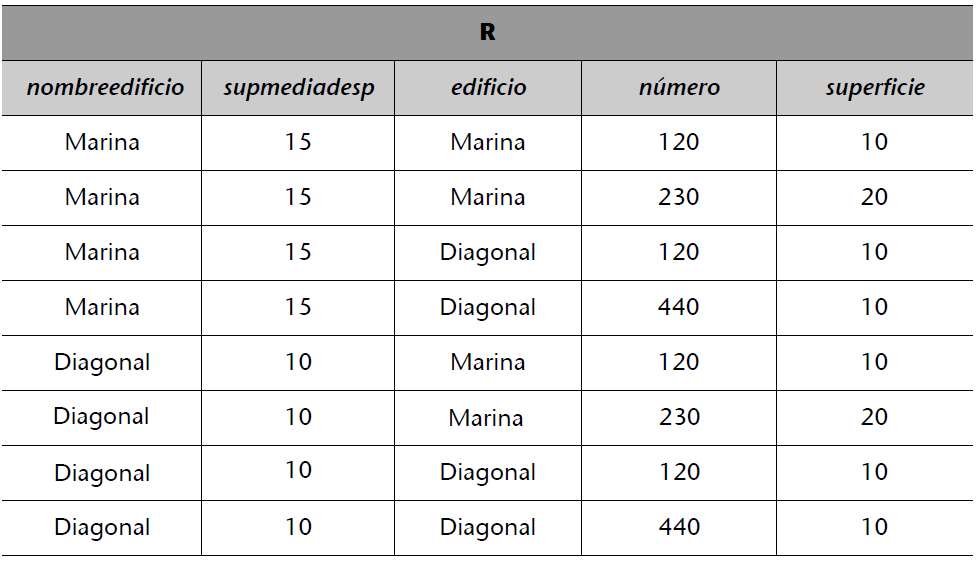
\includegraphics[width=10cm]{imagenes/15_ejemplo7.png}
%\caption{Restultado gr�fico de un producto cartesiano}
%\label{fig:ejemplo7}
%\end{figure}

\begin{table}[h!]
\footnotesize
\centering
\begin{tabular}{|c|c|c|c|c|}
\hline
\multicolumn{5}{|c|}{\textbf{R}}                                                                            \\ \hline
\textit{nombreedificio} & \textit{supmediadesp} & \textit{edificio} & \textit{numero} & \textit{superficie} \\ \hline
Marina                  & 15                    & Marina            & 120             & 10                  \\ \hline
Marina                  & 15                    & Marina            & 230             & 20                  \\ \hline
Marina                  & 15                    & Diagonal          & 120             & 10                  \\ \hline
Marina                  & 15                    & Diagonal          & 440             & 10                  \\ \hline
Diagonal                & 10                    & Marina            & 120             & 10                  \\ \hline
Diagonal                & 10                    & Marina            & 230             & 20                  \\ \hline
Diagonal                & 10                    & Diagonal          & 120             & 10                  \\ \hline
Diagonal                & 10                    & Diagonal          & 440             & 10                  \\ \hline
\end{tabular}
\caption{Restultado gr�fico de un producto cartesiano.}
\label{tab:ejemplo7}
\end{table}

\section{Reunion}
\label{app-reunion}

La presente secci�n contiene distintos ejemplos para cada tipo de \textbf{reuni�n}. Si desea ahondar m�s en la explicaci�n te�rica de esta operaci�n, debe dirigirse la Secci�n \ref{reunion}. \\

Por ejemplo, si se desea encontrar los datos de los despachos que tienen una superficie mayor o igual que la superficie de los despachos del edificio donde est�n situados, entonces se utiliza la operaci�n \textbf{reuni�n} como se muestra en la Consulta \ref{eq:32.1} y \ref{eq:32.2}. \\

\begin{equation}
\rho_{nombreedificio,supmediadesp}\emph{EDIFICIOS\_EMP}
\label{eq:32.1}
\end{equation}
\\
\begin{equation}
\emph{EDIFICIOS\_EMP} \bowtie_{nombreedificio = edificio \wedge supmediadesp \leq superficie}\emph{DESPACHOS}
\label{eq:32.2}
\end{equation}
\\

El resultado gr�fico de la Consulta \ref{eq:32.1} y \ref{eq:32.2} se aprecia en la Tabla \ref{tab:ejemplo8}. Para realizar esta operaci�n, fue necesario cambiar el nombre del atributo $edificio$ de la relaci�n $\emph{EDIFICOS\_EMP}$ por $nombreedificio$, para que no haya problema con el atributo $edificio$ de la relaci�n $\emph{DESPACHOS}$. \\

%\begin{figure}[h!]
%\centering
%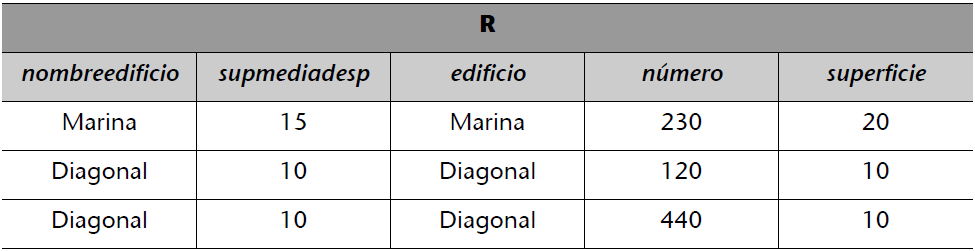
\includegraphics[width=10cm]{imagenes/16_ejemplo8.png}
%\caption{Restultado gr�fico de una reuni�n}
%\label{fig:ejemplo8}
%\end{figure}

\begin{table}[h!]
\footnotesize
\centering
\begin{tabular}{|c|c|c|c|c|}
\hline
\multicolumn{5}{|c|}{\textbf{R}}                                                                            \\ \hline
\textit{nombreedificio} & \textit{supmediadesp} & \textit{edificio} & \textit{numero} & \textit{superficie} \\ \hline
Marina                  & 15                    & Marina            & 120             & 10                  \\ \hline
Diagonal                & 10                    & Diagonal          & 120             & 10                  \\ \hline
Diagonal                & 10                    & Diagonal          & 440             & 10                  \\ \hline
\end{tabular}
\caption{Restultado gr�fico de una reuni�n.}
\label{tab:ejemplo8}
\end{table}

Tal como se explic� en la Secci�n \ref{reunion}, los resultados de una \textbf{reuni�n} con comparaciones de igualdad, o \textbf{equirreuni�n}, siempre tiene uno o m�s pares de atributos con valores id�nticos en todas las tuplas, como se aprecia en la tabla \ref{tab:ejemplo8}, donde los valores de $nombreedificio$ y $edificio$ son iguales para cada tupla. Para evitar esto, se utiliza una \textbf{reuni�n natural} \cite{elmasri2002fundamentos}. \\

Como los atributos sobre los cuales se especifica la \textbf{reuni�n natural} tienen los mismos nombre en ambas relaciones, no hace falta renombrarlos. �sto evita el trabajo hecho en los ejemplos de las Tablas \ref{tab:ejemplo7} y \ref{tab:ejemplo8}, donde se debi� cambiar el nombre del atributo $edificio$ de la relaci�n $\emph{EDIFICIOS\_EMP}$ para que no genere un problema con el atributo $edificio$ de la relaci�n $\emph{DESPACHOS}$ \cite{elmasri2002fundamentos}. \\

Si se hace una \textbf{reuni�n natural} entre $\emph{EDIFICIOS\_EMP}$ y $\emph{DESPACHOS}$, sin la necesidad de renombrar los atributos, se escribe como se muestra en la Consulta \ref{eq:34}. \\

\begin{equation}
\emph{EDIFICIOS\_EMP} \ast \emph{DESPACHOS}
\label{eq:34}
\end{equation}
\\

El resultado gr�fico de la Consulta \ref{eq:34} se aprecia en la Tabla \ref{tab:ejemplo9}. \\

\begin{table}[h!]
\footnotesize
\centering
\begin{tabular}{|c|c|c|c|}
\hline
\multicolumn{4}{|c|}{\textbf{R}}                                                  \\ \hline
\textit{edificio} & \textit{supmediadesp} & \textit{numero} & \textit{superficie} \\ \hline
Marina            & 15                    & 120             & 10                  \\ \hline
Marina            & 15                    & 230             & 20                  \\ \hline
Diagonal          & 10                    & 120             & 10                  \\ \hline
Diagonal          & 10                    & 440             & 10                  \\ \hline
\end{tabular}
\caption{Restultado gr�fico de una reuni�n natural.}
\label{tab:ejemplo9}
\end{table}

\section{Divisi�n}
\label{app-division}

La presente secci�n contiene un ejemplo ilustrativo que explica una \textbf{divisi�n} relacional. Si desea ahondar m�s en la explicaci�n te�rica de la \textbf{divisi�n}, debe leer la Secci�n \ref{div}. \\

Si se tiene una relaci�n llamada $\emph{EDIFICIOS\_EMP}$ que contiene s�lo los nombres de los edificios y otra llamada $\emph{EDIFICIOS\_EMPLEADOS}$ que tiene un historial de los edificios en los cuales han trabajado los empleados, ambas se muestran en la Tabla \ref{tab:ejemplo10}. Si se quiere saber cu�les empleados han trabajado en todos los edificios, se hace una \textbf{divisi�n} entre las relaciones $\emph{EDIFICIOS\_EMP}$ y $\emph{EDIFICIOS\_EMPLEADOS}$. El resultado de esta \textbf{divisi�n} se muestra en la Tabla \ref{tab:ejemplo10.1}. Como se aprecia, tanto \textit{Marta} y \textit{Jorge} son valores de $\emph{EDIFICIOS\_EMPLEADOS}(nombre)$ que aparecen en combinaci�n con todas las tuplas de $\emph{EDIFICIOS}(edificio)$. \\

\begin{table}[h!]
\footnotesize
\centering
\begin{tabular}{|c|c|cc}
\cline{1-2}
\multicolumn{2}{|c|}{\textbf{EDIFICIOS\_EMPLEADOS}} &  &                                  \\ \cline{1-2}
\textit{edificio}      & \textit{nombre}     &  &                                  \\ \cline{1-2}
Marina              & Marta             &  &                                  \\ \cline{1-2}
Diagonal              & Marta             &  &                                  \\ \cline{1-2}
Rosales              & Marta             &  &                                  \\ \cline{1-2} \cline{4-4} 
Almodovar              & Marta             &  & \multicolumn{1}{|c|}{\textbf{EDIFICIOS\_EMP}} \\ \cline{1-2} \cline{4-4} 
Marina              & Carlos             &  & \multicolumn{1}{|c|}{\textit{edificio}} \\ \cline{1-2} \cline{4-4} 
Rosales              & Carlos             &  & \multicolumn{1}{|c|}{Marina}         \\ \cline{1-2} \cline{4-4} 
Diagonal              & Elena             &  & \multicolumn{1}{|c|}{Diagonal}         \\ \cline{1-2} \cline{4-4} 
Rosales              & Elena             &  & \multicolumn{1}{|c|}{Rosales}         \\ \cline{1-2} \cline{4-4} 
Almodovar              & Elena             &  &                                  \\ \cline{1-2}
Marina              & Jorge             &  &                                  \\ \cline{1-2}
Diagonal              & Jorge             &  &                                  \\ \cline{1-2}
Rosales              & Jorge             &  &                                  \\ \cline{1-2}
\end{tabular}
\caption{Relaciones $\emph{EDIFICIOS\_EMPLEADOS}$ Y $\emph{EDIFICIOS\_EMP}$.}
\label{tab:ejemplo10}
\end{table}

\begin{table}[h!]
\footnotesize
\centering
\begin{tabular}{|c|}
\hline
\textbf{R} \\ \hline
\textit{nombre} \\ \hline
Marta         \\ \hline
Jorge         \\ \hline
\end{tabular}
\caption{Resultado de una divisi�n.}
\label{tab:ejemplo10.1}
\end{table}

\section{Funciones Agregadas y de Agrupaci�n}
\label{app-funcagreg}

Esta secci�n contiene un ejemplo de \textbf{agregaci�n} y \textbf{agrupaci�n}. Si desea ahondar m�s en la explicaci�n de estas operaciones, debe leer la Secci�n \ref{funcagreg}. \\

Si deseamos saber la superficie total por cada edificio en la relaci�n $\emph{DESPACHOS}$, entonces se debe agrupar las tuplas por el atributo $edificio$ y luego calcular la suma del atributo $superficie$ de cada tupla agrupada, como se muestra en la Consulta \ref{eq:37}. \\

\begin{equation}
_{edificio}\mathfrak{F}_{suma(superficie)}(\emph{DESPACHOS})
\label{eq:37}
\end{equation}
\\ 

El resultado gr�fico de la Consulta \ref{eq:37} se muestra en la Tabla \ref{tab:ejemplo12}. \\

\begin{table}[h!]
\footnotesize
\centering
\begin{tabular}{|c|c|}
\hline
\multicolumn{2}{|c|}{\textbf{R}}  \\ \hline
\textit{edificio} & \textit{suma} \\ \hline
Marina            & 30            \\ \hline
Diagonal          & 10            \\ \hline
\end{tabular}
\caption{Resultado de una suma con agrupaci�n de atributos.}
\label{tab:ejemplo12}
\end{table}

Si no se especifica el atributo de agrupaci�n, como se muestra en la Consulta \ref{eq:38}, entonces el resultado ser� el que se muestra en la Tabla \ref{tab:ejemplo13}. \\

\begin{equation}
\mathfrak{F}_{suma(superficie)}(\emph{DESPACHOS})
\label{eq:38}
\end{equation}
\\ 

\begin{table}[h!]
\footnotesize
\centering
\begin{tabular}{|c|}
\hline
\textbf{R}    \\ \hline
\textit{suma} \\ \hline
50            \\ \hline
\end{tabular}
\caption{Resultado de una suma sin agrupaci�n de atributos.}
\label{tab:ejemplo13}
\end{table}

\section{Reuni�n Externa}
\label{app-reunionexterna}

Esta secci�n contiene un ejemplo para cada funci�n de reuni�n externa, o sea, \textbf{reuni�n externa izquierda}, \textbf{reuni�n externa derecha} y \textbf{reuni�n externa completa}. Para un estudio a profundidad de la teor�a de estas operaciones, debe dirigirse a la Secci�n \ref{reuexter}. \\

Para hacer una \textbf{reuni�n externa izquierda} entre $\emph{EMPLEADOS\_PROD}$ y $\emph{DESPACHOS}$, renombrado algunos atributos de $\emph{DESPACHO}$, se debe hacer la Consulta \ref{eq:39.1} y \ref{eq:39.2}. Su resultado se muestra en la Tabla \ref{tab:ejemplo14}. \\

\begin{equation}
D \leftarrow \rho_{edificiodesp,numerodesp,superficie}(\emph{DESPACHOS})
\label{eq:39.1}
\end{equation}
\\
\begin{equation}
\emph{EMPLEADOS\_PROD} \leftouterjoin D
\label{eq:39.2}
\end{equation}
\\

\begin{table}[h!]
\footnotesize
\centering
\begin{tabular}{|c|c|c|c|c|c|}
\hline
\multicolumn{6}{|c|}{\textbf{R}}                                                                                            \\ \hline
\textit{ID} & \textit{nombreemp} & \textit{apellidoemp} & \textit{edificiodesp} & \textit{numerodesp} & \textit{superficie} \\ \hline
33.567.711  & Marta              & Roca                 & Marina                & 120                 & 10                  \\ \hline
55.898.425  & Carlos             & Buendia              & Diagonal              & 120                 & 10                  \\ \hline
77.232.144  & Elena              & Pla                  & Marina                & 230                 & 20                  \\ \hline
21.335.245  & Jorge              & Soler                & NULO                  & NULO                & NULO                \\ \hline
88.999.210  & Pedro              & Gonz�lez             & NULO                  & NULO                & NULO                \\ \hline
\end{tabular}
\caption{Resultado de una reuni�n externa izquierda.}
\label{tab:ejemplo14}
\end{table}

Una \textbf{reuni�n externa izquierda} entre $\emph{EMPLEADOS\_PROD}$ y $\emph{DESPACHOS}$, renombrado algunos atributos de $\emph{DESPACHO}$, se hace ejecutando las Consultas \ref{eq:40.1} y \ref{eq:40.2}. Su resultado se muestra en la Tabla \ref{tab:ejemplo15}. \\

\begin{equation}
D \leftarrow \rho_{edificiodesp,numerodesp,superficie}(\emph{DESPACHOS})
\label{eq:40.1}
\end{equation}
\\
\begin{equation}
\emph{EMPLEADOS\_PROD} \rightouterjoin D
\label{eq:40.2}
\end{equation}
\\

\begin{table}[h!]
\footnotesize
\centering
\begin{tabular}{|c|c|c|c|c|c|}
\hline
\multicolumn{6}{|c|}{\textbf{R}}                                                                                            \\ \hline
\textit{ID} & \textit{nombreemp} & \textit{apellidoemp} & \textit{edificiodesp} & \textit{numerodesp} & \textit{superficie} \\ \hline
33.567.711  & Marta              & Roca                 & Marina                & 120                 & 10                  \\ \hline
55.898.425  & Carlos             & Buendia              & Diagonal              & 120                 & 10                  \\ \hline
77.232.144  & Elena              & Pla                  & Marina                & 230                 & 20                  \\ \hline
NULO        & NULO               & NULO                 & Diagonal              & 440                 & 10                  \\ \hline
\end{tabular}
\caption{Resultado de una reuni�n externa derecha.}
\label{tab:ejemplo15}
\end{table}

Por ejemplo, para hacer una \textbf{reuni�n externa completa} entre $\emph{EMPLEADOS\_PROD}$ y $\emph{DESPACHOS}$, renombrado algunos atributos de $\emph{DESPACHO}$, se debe hacer la Consulta que se muestra en la F�rmula \ref{eq:41.1} y \ref{eq:41.2}. Su resultado se muestra en la Tabla \ref{tab:ejemplo16}. \\

\begin{equation}
D \leftarrow \rho_{edificiodesp,numerodesp,superficie}(\emph{DESPACHOS})
\label{eq:41.1}
\end{equation}
\\
\begin{equation}
\emph{EMPLEADOS\_PROD} \fullouterjoin D
\label{eq:41.2}
\end{equation}
\\

\begin{table}[h!]
\footnotesize
\centering
\begin{tabular}{|c|c|c|c|c|c|}
\hline
\multicolumn{6}{|c|}{\textbf{R}}                                                                                            \\ \hline
\textit{ID} & \textit{nombreemp} & \textit{apellidoemp} & \textit{edificiodesp} & \textit{numerodesp} & \textit{superficie} \\ \hline
33.567.711  & Marta              & Roca                 & Marina                & 120                 & 10                  \\ \hline
55.898.425  & Carlos             & Buendia              & Diagonal              & 120                 & 10                  \\ \hline
77.232.144  & Elena              & Pla                  & Marina                & 230                 & 20                  \\ \hline
21.335.245  & Jorge              & Soler                & NULO                  & NULO                & NULO                \\ \hline
88.999.210  & Pedro              & Gonz�lez             & NULO                  & NULO                & NULO                \\ \hline
NULO        & NULO               & NULO                 & Diagonal              & 440                 & 10                  \\ \hline
\end{tabular}
\caption{Resultado de una reuni�n externa completa.}
\label{tab:ejemplo16}
\end{table}

\section{Traducci�n de �lgebra Relacional a SQL}
\label{app-ar2sql}

En esta secci�n se agrega una tabla de traducci�n de �lgebra Relacional a SQL. La explicaci�n del por qu� de esta traducci�n se agrega en la Secci�n \ref{ar2sql}. Esta traducci�n se presenta en la Tabla \ref{tab:ar2sql}, donde cada operaci�n tiene su nombre, su sintaxis en �lgebra Relacional y su sintaxis en SQL. \\

\begin{table}[h!]
\footnotesize
\centering
\begin{tabular}{|p{3.5cm}|p{4cm}|p{7.5cm}|}
\hline
\rowcolor[HTML]{9B9B9B} 
\multicolumn{3}{|l|}{\cellcolor[HTML]{9B9B9B}\textbf{�lgebra Relacional a SQL}}                                                                                                                                   \\ \hline
\rowcolor[HTML]{C0C0C0} 
\textit{Operador}              & \textit{�lgebra Relacional} & \textit{SQL}                                                                                                                                       \\ \hline
Selecci�n                      & $\sigma_{<condicion>}(r)$                           & \begin{tabular}[c]{@{}l@{}}\texttt{SELECT * FROM \textbf{r}}\\ \texttt{\textbf{WHERE condicion}}\end{tabular}                                                                          \\ \hline
Proyecci�n                     & $\pi_{<lista\_atributos>}(r)$                           & \begin{tabular}[c]{@{}l@{}}\texttt{SELECT}\\ \texttt{\textbf{lista\_atributos}}\\ \texttt{FROM \textbf{r}}\end{tabular}                                                                \\ \hline
Renombrar                      & $\rho_{s(<lista\_atributos>)}(r)$                           & \begin{tabular}[c]{@{}l@{}}\texttt{SELECT * FROM}\\ \texttt{\textbf{r AS s(lista\_atributos})}\end{tabular}                                                                   \\ \hline
Uni�n                          & $r \cup s$                           & \begin{tabular}[c]{@{}l@{}}\texttt{SELECT * FROM \textbf{r}}\\ \texttt{\textbf{UNION}}\\ \texttt{SELECT * FROM \textbf{s}}\end{tabular}                                                                  \\ \hline
Intersecci�n                   & $r \cap s$                           & \begin{tabular}[c]{@{}l@{}}\texttt{SELECT * FROM \textbf{r}}\\ \texttt{\textbf{INTERSECT}}\\ \texttt{SELECT * FROM \textbf{s}}\end{tabular}                                                              \\ \hline
Diferencia                     & $r - s$                           & \begin{tabular}[c]{@{}l@{}}\texttt{SELECT * FROM \textbf{r}}\\ \texttt{\textbf{EXCEPT}}\\ \texttt{SELECT * FROM \textbf{s}}\end{tabular}                                                                 \\ \hline
Producto Cartesiano            & $r \times s$                           & \begin{tabular}[c]{@{}l@{}}\texttt{SELECT * FROM}\\ \texttt{\textbf{r, s}}\end{tabular}                                                                                       \\ \hline
Reuni�n                        & $r \bowtie s$                           & \begin{tabular}[c]{@{}l@{}}\texttt{SELECT * FROM}\\ \texttt{\textbf{r INNER JOIN s}}\end{tabular}                                                                             \\ \hline
Reuni�n Natural                & $r \ast s$                           & \begin{tabular}[c]{@{}l@{}}\texttt{SELECT * FROM} \\ \texttt{\textbf{r NATURAL JOIN s}}\end{tabular}                                                                          \\ \hline
Divisi�n                       & $r \div s$                           & \begin{tabular}[c]{@{}p{7.5cm}@{}}\texttt{SELECT a FROM r}\\ \texttt{WHERE b IN (SELECT b FROM s)}\\ \texttt{GROUP BY A}\\ \texttt{HAVING COUNT (*) = (SELECT COUNT (*) FROM s)}\end{tabular} \\ \hline
Reuni�n Externa Izquierda      & $r \leftouterjoin s$                          & \begin{tabular}[c]{@{}l@{}}\texttt{SELECT * FROM}\\ \texttt{\textbf{r LEFT OUTER JOIN s}}\end{tabular}                                                                        \\ \hline
Reuni�n Externa Derecha        & $r \rightouterjoin s$                           & \begin{tabular}[c]{@{}l@{}}\texttt{SELECT * FROM}\\ \texttt{\textbf{r RIGHT OUTER JOIN s}}\end{tabular}                                                                       \\ \hline
Reuni�n Externa Completa       & $r \fullouterjoin s$                           & \begin{tabular}[c]{@{}l@{}}\texttt{SELECT * FROM}\\ \texttt{\textbf{r FULL OUTER JOIN s}}\end{tabular}                                                                        \\ \hline
\end{tabular}
\caption{Traducci�n de �lgebra Relacional a SQL.}
\label{tab:ar2sql}
\end{table}
\chapter{Casos de Usos Extendidos}
\label{casosdeusosextendidos}

En este ap�ndice se muestran todos y cada uno de los Casos de Usos pertenecientes a la aplicaci�n a desarrollar. La Tabla \ref{tab:casosdeusos} contiene una lista de todos los Casos de Usos, cada uno con un identificador, el nombre del caso de uso, la referencia a la tabla que contiene el Caso de Uso Extendido, la referencia a la figura que contiene el diagrama de secuencia y la referencia a la figura que contiene el diagrama de estados. \\

% Please add the following required packages to your document preamble:
% \usepackage[table,xcdraw]{xcolor}
% If you use beamer only pass "xcolor=table" option, i.e. \documentclass[xcolor=table]{beamer}
\begin{table}[h!]
\footnotesize
\centering
\begin{tabular}{|p{1cm}|p{3.5cm}|p{3.5cm}|p{3.5cm}|p{3.5cm}|}
\hline
\rowcolor[HTML]{9B9B9B} 
\multicolumn{5}{|l|}{\cellcolor[HTML]{9B9B9B}\textbf{Lista de Casos de Usos.}}                                                               \\ \hline
\rowcolor[HTML]{C0C0C0} 
\textit{Id} & \textit{Nombre}      & \textit{Caso de Uso Extendido} & \textit{Diagrama de Secuencia} & \textit{Diagrama de Estados} \\ \hline
CU01        & Ir Inicio            & Tabla \ref{tab:cuirinicio}                        & Figura \ref{fig:secirinicio}                       & Figura \ref{fig:estirinicio}                     \\ \hline
CU02        & Iniciar Sesi�n       & Tabla \ref{tab:cuiniciarsesion}                        & Figura \ref{fig:seciniciarsesion}                       & Figura \ref{fig:estiniciarsesion}                     \\ \hline
CU03        & Sesi�n Profesor      & Tabla \ref{tab:cusesionprofesor}                        & Figura \ref{fig:secsesionprofesor}                       & Figura \ref{fig:estsesionprofesor}                     \\ \hline
CU04        & Gestionar Cuentas   & Tabla \ref{tab:cugestionarcuentas}                        & Figura \ref{fig:secgestionarcuentas}                       & Figura \ref{fig:estgestionarcuentas}                     \\ \hline
CU05        & Crear Cuenta Alumno         & Tabla \ref{tab:cucrearcuenta}                        & Figura \ref{fig:seccrearcuenta}                       & Figura \ref{fig:estcrearcuenta}                     \\ \hline
CU06        & Eliminar Cuenta      & Tabla \ref{tab:cueliminarcuenta}                        & Figura \ref{fig:seceliminarcuenta}                       & Figura \ref{fig:esteliminarcuenta}                     \\ \hline
CU07        & Modificar Cuenta     & Tabla \ref{tab:cumodificarcuenta}                        & Figura \ref{fig:secmodificarcuenta}                       & Figura \ref{fig:secmodificarcuenta}                     \\ \hline
CU08        & Gestionar BD         & Tabla \ref{tab:cugestionarbd}                        & Figura \ref{fig:secgestionarbd}                       & Figura \ref{fig:estgestionarbd}                     \\ \hline
CU09        & Crear BD             & Tabla \ref{tab:cucrearbd}                        & Figura \ref{fig:seccrearbd}                       & Figura \ref{fig:estcrearbd}                     \\ \hline
CU10        & Eliminar BD          & Tabla \ref{tab:cueliminarbd}                        & Figura \ref{fig:seceliminarbd}                       & Figura \ref{fig:esteliminarbd}                     \\ \hline
CU11        & Modificar BD         & Tabla \ref{tab:cumodificarbd}                        & Figura \ref{fig:secmodificarbd}                       & Figura \ref{fig:estmodificarbd}                     \\ \hline
%CU12        & Guardar BD           & Tabla \ref{tab:cuguardarbd}                        & Figura \ref{fig:secguardarbd}                       & Figura \ref{fig:estguardarbd}                     \\ \hline
CU12        & Cargar BD            & Tabla \ref{tab:cucargarbd}                        & Figura \ref{fig:seccargarbd}                       & Figura \ref{fig:estcargarbd}                     \\ \hline
CU13        & Gestionar Ejercicios & Tabla \ref{tab:cugestionarejercicios}                        & Figura \ref{fig:secgestionarejercicios}                       & Figura \ref{fig:estgestionarejercicios}                     \\ \hline
CU14        & Crear Ejercicios     & Tabla \ref{tab:cucrearejercicios}                        & Figura \ref{fig:secgestionarejercicios}                       & Figura \ref{fig:estgestionarejercicios}                     \\ \hline
CU15        & Eliminar Ejercicios  & Tabla \ref{tab:cueliminarejercicios}                        & Figura \ref{fig:seceliminarejercicios}                       & Figura \ref{fig:esteliminarejercicios}                     \\ \hline
CU16        & Modificar Ejercicios & Tabla \ref{tab:cueliminarejercicios}                        & Figura \ref{fig:seceliminarejercicios}                       & Figura \ref{fig:esteliminarejercicios}                     \\ \hline
CU17        & Responder Ejercicios & Tabla \ref{tab:curesponderejercicios}                        & Figura \ref{fig:secresponderejercicios}                       & Figura \ref{fig:estresponderejercicios}                     \\ \hline
CU18        & Gestionar Relaci�n   & Tabla \ref{tab:cugestionarrelacion}                        & Figura \ref{fig:secgestionarrelacion}                       & Figura \ref{fig:estgestionarrelacion}                     \\ \hline
CU19        & Agregar Relaci�n     & Tabla \ref{tab:cuagregarrelacion}                        & Figura \ref{fig:secagregarrelacion}                       & Figura \ref{fig:estagregarrelacion}                     \\ \hline
CU20        & Eliminar Relaci�n    & Tabla \ref{tab:cueliminarrelacion}                        & Figura \ref{fig:seceliminarrelacion}                       & Figura \ref{fig:esteliminarrelacion}                     \\ \hline
CU21        & Modificar Relaci�n   & Tabla \ref{tab:cumodificarrelacion}                        & Figura \ref{fig:secmodificarrelacion}                       & Figura \ref{fig:estmodificarrelacion}                     \\ \hline
CU22        & Ver Relaci�n         & Tabla \ref{tab:cuverrelacion}                        & Figura \ref{fig:secverrelacion}                       & Figura \ref{fig:estverrelacion}                     \\ \hline
CU23        & Gestionar Tupla      & Tabla \ref{tab:cugestionartupla}                        & Figura \ref{fig:secgestionartupla}                       & Figura \ref{fig:estgestionartupla}                     \\ \hline
CU24        & Ingresar Tupla        & Tabla \ref{tab:cuagregartupla}                        & Figura \ref{fig:secagregartupla}                       & Figura \ref{fig:estagregartupla}                     \\ \hline
CU25        & Eliminar Tupla       & Tabla \ref{tab:cueliminartupla}                        & Figura \ref{fig:seceliminartupla}                       & Figura \ref{fig:esteliminartupla}                     \\ \hline
CU26        & Modificar Tupla      & Tabla \ref{tab:cumodificartupla}                        & Figura \ref{fig:secmodificartupla}                       & Figura \ref{fig:estmodificartupla}                     \\ \hline
CU27        & Sesi�n Alumno        & Tabla \ref{tab:cusesionalumno}                        & Figura \ref{fig:secsesionalumno}                       & Figura \ref{fig:estsesionalumno}                     \\ \hline
CU28        & Hacer Consulta       & Tabla \ref{tab:cuhacerconsulta}                        & Figura \ref{fig:sechacerconsulta}                      & Figura \ref{fig:esthacerconsulta}                     \\ \hline
CU29        & Ver Estad�sticas     & Tabla \ref{tab:cuverestadisticas}                        & Figura \ref{fig:secverestadisticas}                       & Figura \ref{fig:estverestadisticas}                     \\ \hline
\end{tabular}
\caption{Lista de Casos de Usos.}
\label{tab:casosdeusos}
\end{table}

% Ir Inicio
\clearpage
\begin{table}[h!]
\footnotesize
\centering
\begin{tabular}{|p{7.5cm}|p{7.5cm}|}
\hline
\rowcolor[HTML]{C0C0C0} 
\textbf{Caso de Uso}                                                                                                                  & \textbf{ID: CU01}                                                               \\ \hline
\textbf{Nombre}                                                                                                                       & Ir Inicio                                                                       \\ \hline
\textbf{Actores}                                                                                                                      & Usuario (Alumno y Profesor)                                                               \\ \hline
\textbf{Prop�sito}                                                                                                                    & Crear cuenta de alumno e iniciar sesi�n desde la p�gina de inicio                         \\ \hline
\textbf{Resumen}                                                                                                                      & El alumno o el profesor elige una opci�n que se muestra en la pagina de inicio \\ \hline
\rowcolor[HTML]{EFEFEF} 
\textbf{Curso Normal (Usuario)}                                                                                                       & \textbf{Curso Normal (Sistema)}                                                 \\ \hline
1. El usuario ingresa a la p�gina de inicio                                                                                       &                                                                                 \\ \hline
2. El usuario puede seleccionar entre Crear Cuenta Alumno (ver Tabla \ref{tab:cucrearcuenta}); b. Iniciar Sesi�n (ver Tabla \ref{tab:cuiniciarsesion}) &                                                                                 \\ \hline
\rowcolor[HTML]{EFEFEF} 
\textbf{Curso Alternativo (Usuario)}                                                                                                  & \textbf{Curso Alternativo (Sistema)}                                            \\ \hline
                                                                                                                                      & Paso 1: Si el sistema no muestra la pagina de inicio, arrojar� un mensaje de error.                        \\ \hline
\end{tabular}
\caption{Caso de Uso Extendido - Ir Inicio.}
\label{tab:cuirinicio}
\end{table}

\begin{figure}[h!]
\centering
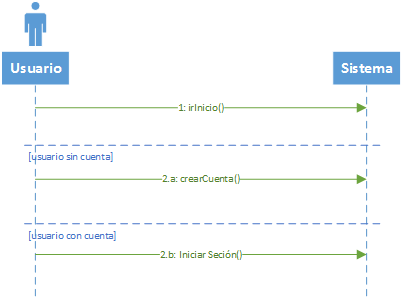
\includegraphics[width=10cm]{imagenes/secuencia_ir_inicio.png}
\caption{Diagrama de Secuencia - Ir Inicio.}
\label{fig:secirinicio}
\end{figure}

\begin{figure}[h!]
\centering
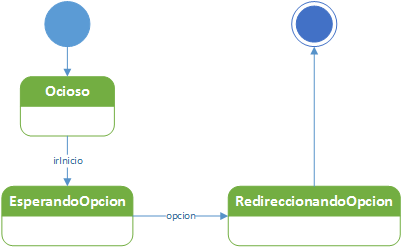
\includegraphics[width=7cm]{imagenes/estado_ir_inicio.png}
\caption{Diagrama de Estados - Ir Inicio.}
\label{fig:estirinicio}
\end{figure}

% Iniciar Sesi�n
\clearpage
\begin{table}[h!]
\footnotesize
\centering
\begin{tabular}{|p{7.5cm}|p{7.5cm}|}
\hline
\rowcolor[HTML]{C0C0C0} 
\textbf{Secci�n Iniciar Sesi�n}                    & \textbf{ID: CU02}                                                                                                                                                                                              \\ \hline
\rowcolor[HTML]{EFEFEF} 
\textbf{Curso Normal (Usuario)}                    & \textbf{Curso Normal (Sistema)}                                                                                                                                                                                  \\ \hline
1. El usuario ingresa su correo y contrase�a       &                                                                                                                                                                                                                  \\ \hline
                                                   & 2. El sistema valida los datos del usuario y carga la sesi�n                                                                                                                                                     \\ \hline
                                                   & 3. El sistema redirecciona dependiendo del usuario que ingrese: a. Sesi�n Profesor, si el usuario corresponde a un profesor (ver Tabla \ref{tab:cusesionprofesor}); b. Sesi�n Alumno, si el usuario corresponde a un alumno (ver Tabla \ref{tab:cusesionalumno}) \\ \hline
\rowcolor[HTML]{EFEFEF} 
\textbf{Curso Alternativo (Usuario)}               & \textbf{Curso Alternativo (Sistema)}                                                                                                                                                                             \\ \hline
                                                   & Paso 2: Si los datos ingresados no son los correctos, el sistema indica dicho acontecimiento y vuelve al paso 1                                                                                                  \\ \hline
                                                   & Paso 3: Si el sistema no logra redireccionar, manda un mensaje de error                                                                                                                                          \\ \hline
\end{tabular}
\caption{Caso de Uso Extendido - Iniciar Sesi�n.}
\label{tab:cuiniciarsesion}
\end{table}

\begin{figure}[h!]
\centering
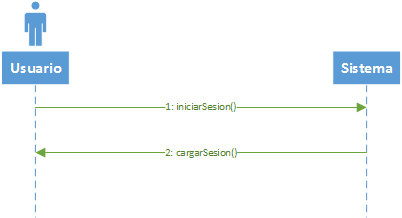
\includegraphics[width=10cm]{imagenes/secuencia_iniciar_sesion.png}
\caption{Diagrama de Secuencia - Iniciar Sesi�n.}
\label{fig:seciniciarsesion}
\end{figure}

\begin{figure}[h!]
\centering
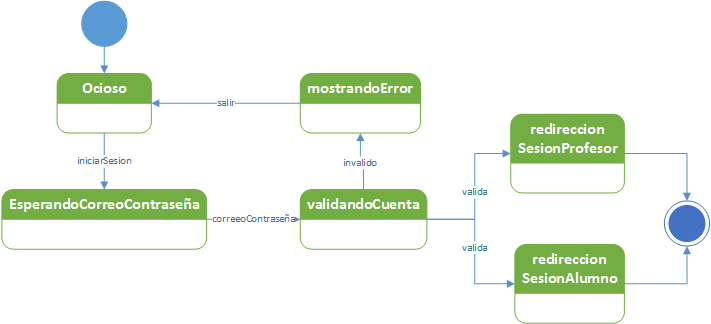
\includegraphics[width=15cm]{imagenes/estado_iniciar_sesion.png}
\caption{Diagrama de Estados - Iniciar Sesi�n.}
\label{fig:estiniciarsesion}
\end{figure}

% Sesion Profesor
\clearpage
\begin{table}[h!]
\footnotesize
\centering
\begin{tabular}{|p{7.5cm}|p{7.5cm}|}
\hline
\rowcolor[HTML]{C0C0C0} 
\textbf{Caso de Uso}                                                                                                                                                                                                                                                                                                                & \textbf{ID: CU03}                                                                                                                                                 \\ \hline
\textbf{Nombre}                                                                                                                                                                                                                                                                                                                     & Sesi�n Profesor                                                                                                                                                   \\ \hline
\textbf{Actores}                                                                                                                                                                                                                                                                                                                    & Profesor                                                                                                                                                          \\ \hline
\textbf{Prop�sito}                                                                                                                                                                                                                                                                                                                  & Mostrar al Profesor todas las opciones que tiene disponibles \\ \hline
\textbf{Resumen}                                                                                                                                                                                                                                                                                                                    & El Profesor elige una opci�n que se muestra en el men� de sesi�n de profesor                                                                                      \\ \hline
\rowcolor[HTML]{EFEFEF} 
\textbf{Curso Normal (Usuario)}                                                                                                                                                                                                                                                                                                     & \textbf{Curso Normal (Sistema)}                                                                                                                                   \\ \hline
1. El profesor ingresa al sistema desde el Caso de Uso \ref{tab:cuiniciarsesion} Iniciar Sesi�n                                                                                                                                                                                                                                                             &                                                                                                                                                                   \\ \hline
2. El profesor selecciona alguna opci�n: a. Gestionar Cuentas (ver Tabla \ref{tab:cugestionarcuentas}); b. Modificar Cuenta(ver Tabla \ref{tab:cumodificarcuenta}); c. Gestionar BD (ver Tabla \ref{tab:cugestionarbd}); d. Gestionar Relaciones (ver Tabla \ref{tab:cugestionarrelacion}); e. Gestionar Tuplas (ver Tabla \ref{tab:cugestionartupla}); f: Gestionar Ejercicios (var Tabla \ref{tab:cugestionarejercicios}); g. Hacer Consulta (ver Tabla \ref{tab:cuhacerconsulta}); h. Ver Estad�sticas (ver Tabla \ref{tab:cuverestadisticas}) &                                                                                                                                                                   \\ \hline
                                                                                                                                                                                                                                                                                                                                    & 3. El sistema direcciona a la opci�n correspondiente                                                                                                           \\ \hline
\rowcolor[HTML]{EFEFEF} 
\textbf{Curso Alternativo (Usuario)}                                                                                                                                                                                                                                                                                                & \textbf{Curso Alternativo (Sistema)}                                                                                                                              \\ \hline
                                                                                                                                                                                                                                                                                                                                    & Paso 3: si no se puede direccionar, se muestra un error                                                                                                          \\ \hline
\end{tabular}
\caption{Caso de Uso Extendido - Sesi�n Profesor.}
\label{tab:cusesionprofesor}
\end{table}

\begin{figure}[h!]
\centering
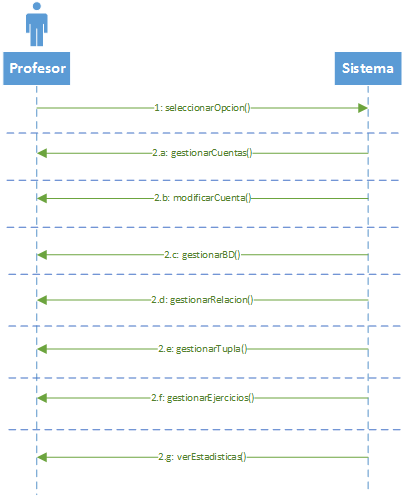
\includegraphics[width=10cm]{imagenes/secuencia_sesion_profesor.png}
\caption{Diagrama de Secuencia - Sesi�n Profesor.}
\label{fig:secsesionprofesor}
\end{figure}

\begin{figure}[h!]
\centering
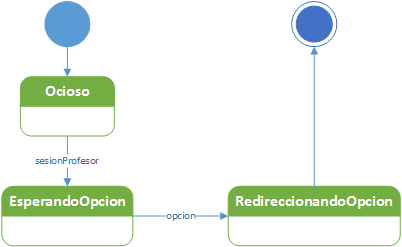
\includegraphics[width=7cm]{imagenes/estado_sesion_profesor.png}
\caption{Diagrama de Estados - Sesi�n Profesor.}
\label{fig:estsesionprofesor}
\end{figure}

% Gestionar Cuentas
\clearpage
\begin{table}[h!]
\footnotesize
\centering
\begin{tabular}{|p{7.5cm}|p{7.5cm}|}
\hline
\rowcolor[HTML]{C0C0C0} 
\textbf{Caso de Uso}                                                                                                                                          & \textbf{ID: CU04}                                                                                               \\ \hline
\textbf{Nombre}                                                                                                                                               & Gestionar Usuario                                                                                               \\ \hline
\textbf{Actores}                                                                                                                                              & Profesor                                                                                                        \\ \hline
\textbf{Prop�sito}                                                                                                                                            & Mostrar al Profesor todas las opciones de Gesti�n de Usuarios: Crear Cuenta, Eliminar Cuenta, Modificar Cuenta \\ \hline
\textbf{Resumen}                                                                                                                                              & El Profesor elige una opci�n que se muestra en el men� de gesti�n de usuarios                                  \\ \hline
\rowcolor[HTML]{EFEFEF} 
\textbf{Curso Normal (Usuario)}                                                                                                                               & \textbf{Curso Normal (Sistema)}                                                                                 \\ \hline
1. El profesor ingresa al men� Gestionar Cuentas &                                                                                                                 \\ \hline
2. El profesor selecciona alguna opci�n: a. Crear Cuenta (ver Tabla \ref{tab:cucrearcuenta}); b. Eliminar Cuenta (ver Tabla \ref{tab:cueliminarcuenta}); c. Modificar Cuenta (ver Tabla \ref{tab:cumodificarcuenta}) &                                                                                                                 \\ \hline
                                                                                                                                                              & 3. El sistema direcciona a la opci�n correspondiente                                                           \\ \hline
\rowcolor[HTML]{EFEFEF} 
\textbf{Curso Alternativo (Usuario)}                                                                                                                          & \textbf{Curso Alternativo (Sistema)}                                                                            \\ \hline
                                                                                                                                                              & Paso 3: Si el sistema no logra direccionar, se muestra un error                                                        \\ \hline
\end{tabular}
\caption{Caso de Uso Extendido - Gestionar Cuentas.}
\label{tab:cugestionarcuentas}
\end{table}

\begin{figure}[h!]
\centering
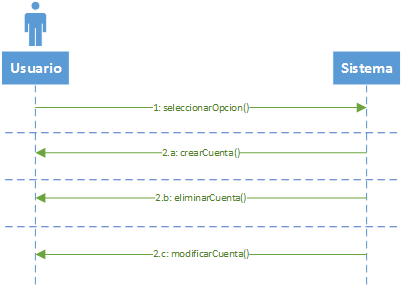
\includegraphics[width=10cm]{imagenes/secuencia_gestionar_usuarios.png}
\caption{Diagrama de Secuencia - Gestionar Cuentas.}
\label{fig:secgestionarcuentas}
\end{figure}

\begin{figure}[h!]
\centering
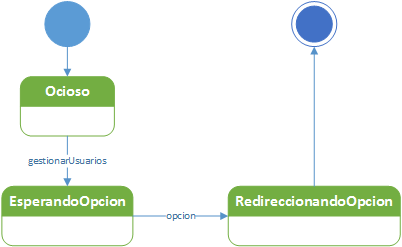
\includegraphics[width=7cm]{imagenes/estado_gestionar_usuarios.png}
\caption{Diagrama de Estados - Gestionar Cuentas.}
\label{fig:estgestionarcuentas}
\end{figure}

% Crear Cuenta
\clearpage
\begin{table}[h!]
\footnotesize
\centering
\begin{tabular}{|p{7.5cm}|p{7.5cm}|}
\hline
\rowcolor[HTML]{C0C0C0} 
\textbf{Secci�n Crear Cuenta Alumno}                      & \textbf{ID: CU05}                                                                                                                                                                                                                                                                                                     \\ \hline
\rowcolor[HTML]{EFEFEF} 
\textbf{Curso Normal (Usuario)}                    & \textbf{Curso Normal (Sistema)}                                                                                                                                                                                                                                                                                       \\ \hline
1. El usuario selecciona la opci�n Crear Cuenta Alumno    &                                                                                                                                                                                                                                                                                                                       \\ \hline
2. El usuario ingresa los datos de la nueva cuenta &                                                                                                                                                                                                                                                                                                                       \\ \hline
                                                   & 3. El sistema valida los datos del usuario y se registra la nueva cuenta                                                                                                                                                                                                                                              \\ \hline
                                                   & 4. El sistema muestra un mensaje al usuario indicando que se ha creado la nueva cuenta y redirecciona dependiendo del usuario que ingrese: a. Ir Inicio, si el usuario lleg� por el men� inicial (ver Tabla \ref{tab:cuirinicio}); b. Gestionar Cuentas, si el usuario lleg� desde el men� Gestionar Cuentas (ver Tabla \ref{tab:cugestionarcuentas}) \\ \hline
\rowcolor[HTML]{EFEFEF} 
\textbf{Curso Alternativo (Usuario)}               & \textbf{Curso Alternativo (Sistema)}                                                                                                                                                                                                                                                                                  \\ \hline
                                                   & Paso 3: Si los datos ingresados no son los correctos, el sistema indica dicho acontecimiento y vuelve al paso 1                                                                                                                                                                                                       \\ \hline
                                                   & Paso 4: Si el sistema no logra redireccionar, manda un mensaje de error                                                                                                                                                                                                                                               \\ \hline
\end{tabular}
\caption{Caso de Uso Extendido - Crear Cuenta Alumno.}
\label{tab:cucrearcuenta}
\end{table}

\begin{figure}[h!]
\centering
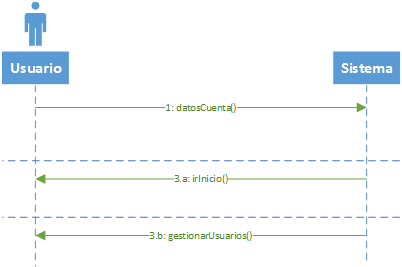
\includegraphics[width=10cm]{imagenes/secuencia_crear_cuenta.png}
\caption{Diagrama de Secuencia - Crear Cuenta Alumno.}
\label{fig:seccrearcuenta}
\end{figure}

\begin{figure}[h!]
\centering
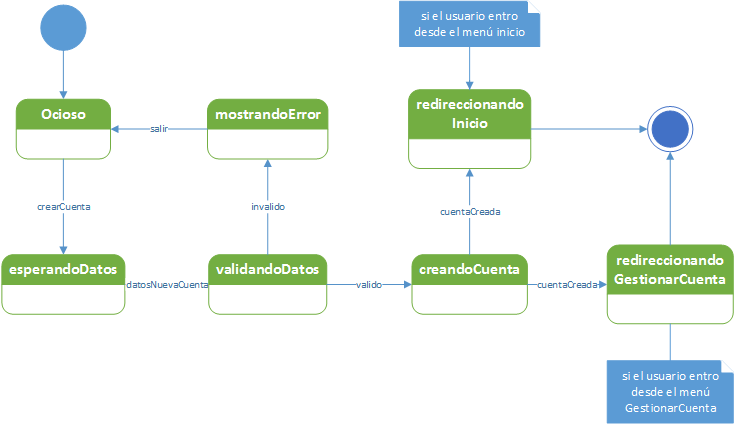
\includegraphics[width=15cm]{imagenes/estado_crear_cuenta.png}
\caption{Diagrama de Estados - Crear Cuenta Alumno.}
\label{fig:estcrearcuenta}
\end{figure}

%Eliminar Cuenta
\clearpage
\begin{table}[h!]
\footnotesize
\centering
\begin{tabular}{|p{7.5cm}|p{7.5cm}|}
\hline
\rowcolor[HTML]{C0C0C0} 
\textbf{Secci�n Eliminar Cuenta}                                                              & \textbf{ID: CU06}                                                                                                                                                                           \\ \hline
\rowcolor[HTML]{EFEFEF} 
\textbf{Curso Normal (Usuario)}                                                               & \textbf{Curso Normal (Sistema)}                                                                                                                                                             \\ \hline
1. El usuario selecciona la opci�n Eliminar Cuenta                                            &                                                                                                                                                                                             \\ \hline
2. El usuario selecciona la cuenta a eliminar                                                 &                                                                                                                                                                                             \\ \hline
                                                                                              & 3. El sistema solicita la confirmaci�n de la eliminaci�n                                                                                                                                    \\ \hline
4. El usuario confirma y acepta la eliminaci�n                                                &                                                                                                                                                                                             \\ \hline
                                                                                              & 5. El sistema elimina la cuenta seleccionada                                                                                                                                                \\ \hline
                                                                                              & 6. El sistema muestra un mensaje al usuario indicando que se ha eliminado la cuenta y redirecciona a la Sesi�n Profesor (ver Tabla \ref{tab:cusesionprofesor})                                                 \\ \hline
\rowcolor[HTML]{EFEFEF} 
\textbf{Curso Alternativo (Usuario)}                                                          & \textbf{Curso Alternativo (Sistema)}                                                                                                                                                        \\ \hline
Paso 4: El usuario no acepta la confirmaci�n, se termina dicho proceso y se vuelve al paso 1 &                                                                                                                                                                                             \\ \hline
                                                                                              & Paso 5: Si el sistema no logra eliminar la cuenta, indica dicho acontecimiento y vuelve al paso 1                                                                                          \\ \hline
                                                                                              & Paso 6: Si el sistema no logra redireccionar, manda un mensaje de error                                                                                                                     \\ \hline
\end{tabular}
\caption{Caso de Uso Extendido - Eliminar Cuenta.}
\label{tab:cueliminarcuenta}
\end{table}

\begin{figure}[h!]
\centering
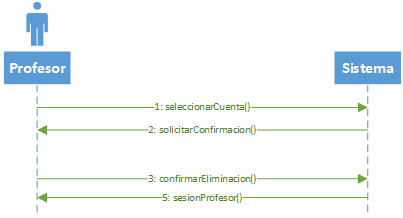
\includegraphics[width=10cm]{imagenes/secuencia_eliminar_cuenta.png}
\caption{Diagrama de Secuencia - Eliminar Cuenta.}
\label{fig:seceliminarcuenta}
\end{figure}

\begin{figure}[h!]
\centering
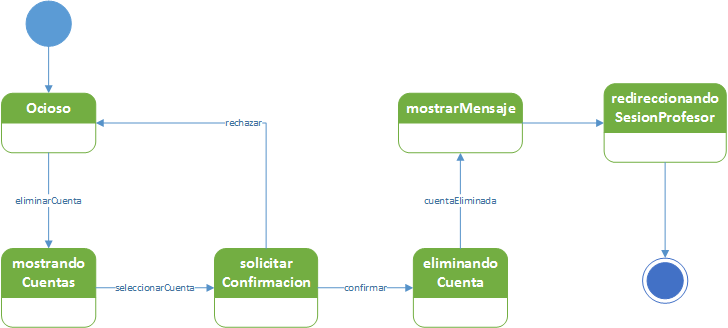
\includegraphics[width=15cm]{imagenes/estado_eliminar_cuenta.png}
\caption{Diagrama de Estados - Eliminar Cuenta.}
\label{fig:esteliminarcuenta}
\end{figure}

% Modificar Cuenta
\clearpage
\begin{table}[h!]
\footnotesize
\centering
\begin{tabular}{|p{7.5cm}|p{7.5cm}|}
\hline
\rowcolor[HTML]{C0C0C0} 
\textbf{Secci�n Modificar Cuenta}                                                              & \textbf{ID: CU07}                                                                                                                            \\ \hline
\rowcolor[HTML]{EFEFEF} 
\textbf{Curso Normal (Usuario)}                                                               & \textbf{Curso Normal (Sistema)}                                                                                                              \\ \hline
1. El usuario selecciona la opci�n Modificar Cuenta                                           &                                                                                                                                              \\ \hline
2. El usuario selecciona la cuenta a modificar                                                &                                                                                                                                              \\ \hline
                                                                                              & 3. El sistema muestra por pantalla los datos de la cuenta seleccionada                                                              \\ \hline
4. El usuario modifica los campos de dicha cuenta y acepta los cambios                        &                                                                                                                                              \\ \hline
                                                                                              & 5. El sistema valida los nuevos datos y solicita confirmaci�n para ejecutar la modificaci�n                                                  \\ \hline
6. El usuario confirma y acepta la modificaci�n                                               &                                                                                                                                              \\ \hline
                                                                                              & 7. El sistema modifica la cuenta seleccionada                                                                                                \\ \hline
                                                                                              & 8. El sistema muestra un mensaje al usuario indicando que se ha modificado la cuenta y redirecciona a la Sesi�n Profesor (ver Tabla \ref{tab:cusesionprofesor}) \\ \hline
\rowcolor[HTML]{EFEFEF} 
\textbf{Curso Alternativo (Usuario)}                                                          & \textbf{Curso Alternativo (Sistema)}                                                                                                         \\ \hline
                                                                                              & Paso 5: Si los datos ingresados no son los correctos o inv�lidos, el sistema indica dicho acontecimiento y vuelve al paso 1                             \\ \hline
Paso 6: El usuario no acepta la confirmaci�n, se termina dicho proceso y se vuelve al paso 1 &                                                                                                                                              \\ \hline
                                                                                              & Paso 7: Si el sistema no logra modificar la cuenta, indica dicho acontecimiento y vuelve al paso 1                                          \\ \hline
                                                                                              & Paso 8: Si el sistema no logra redireccionar, manda un mensaje de error                                                                      \\ \hline
\end{tabular}
\caption{Caso de Uso Extendido - Modificar Cuenta.}
\label{tab:cumodificarcuenta}
\end{table}

\begin{figure}[h!]
\centering
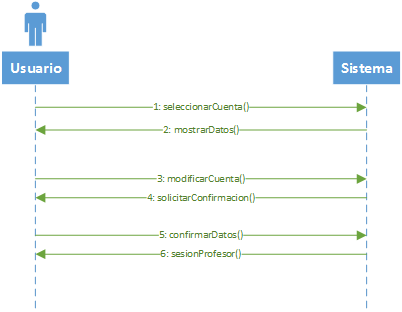
\includegraphics[width=10cm]{imagenes/secuencia_modificar_cuenta.png}
\caption{Diagrama de Secuencia - Modificar Cuenta.}
\label{fig:secmodificarcuenta}
\end{figure}

\begin{figure}[h!]
\centering
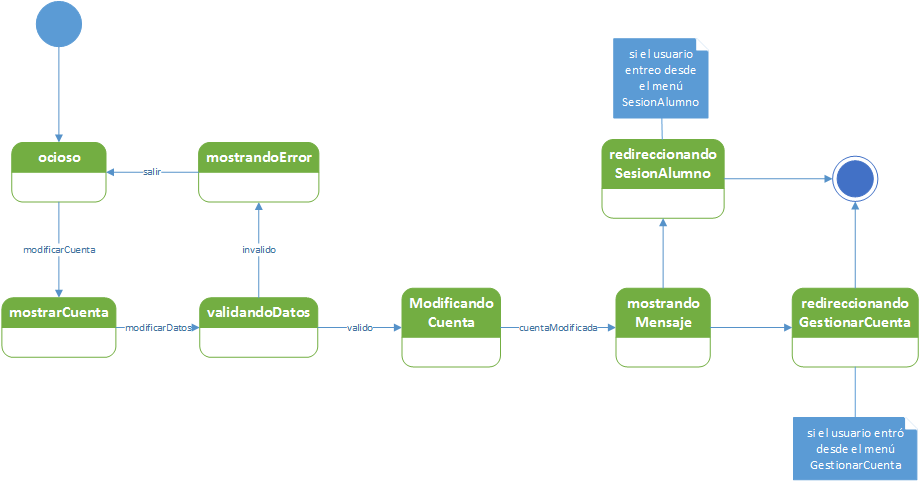
\includegraphics[width=15cm]{imagenes/estado_modificar_cuenta.png}
\caption{Diagrama de Estados - Modificar Cuenta.}
\label{fig:estmodificarcuenta}
\end{figure}

% Gestionar BD
\clearpage
\begin{table}[h!]
\footnotesize
\centering
\begin{tabular}{|p{7.5cm}|p{7.5cm}|}
\hline
\rowcolor[HTML]{C0C0C0} 
\textbf{Caso de Uso}                                                                                                                                                                                                                                                & \textbf{ID: CU08}                                                                                                                         \\ \hline
\textbf{Nombre}                                                                                                                                                                                                                                                     & Gestionar BD                                                                                                                              \\ \hline
\textbf{Actores}                                                                                                                                                                                                                                                    & Profesor \\ \hline
\textbf{Prop�sito}                                                                                                                                                                                                                                                  & Mostrar al Profesor todas las opciones de Gesti�n de BD: Crear BD, Eliminar BD, Modificar BD y Cargar BD \\ \hline
\textbf{Resumen}                                                                                                                                                                                                                                                    & El Profesor elige una opci�n que se muestra en el men� de gesti�n de base de datos                                                        \\ \hline
\rowcolor[HTML]{EFEFEF} 
\textbf{Curso Normal (Usuario)}                                                                                                                                                                                                                                     & \textbf{Curso Normal (Sistema)}                                                                                                           \\ \hline
1. El profesor ingresa al men� Gestionar BD desde el Caso de Uso \ref{tab:cusesionprofesor} Sesi�n Profesor &                                                                                                                                           \\ \hline
2. El usuario selecciona alguna opci�n: a. Crear BD (ver Tabla \ref{tab:cucrearbd}); b. Eliminar BD (ver Tabla \ref{tab:cueliminarbd}); c. Modificar BD (ver Tabla \ref{tab:cumodificarbd}); d. Cargar BD (ver Tabla \ref{tab:cucargarbd}) &                                                                                                                                           \\ \hline
                                                                                                                                                                                                                                                                    & 3. El sistema direcciona a la opci�n correspondiente                                                                                     \\ \hline
\rowcolor[HTML]{EFEFEF} 
\textbf{Curso Alternativo (Usuario)}                                                                                                                                                                                                                                & \textbf{Curso Alternativo (Sistema)}                                                                                                      \\ \hline
                                                                                                                                                                                                                                                                    & Paso 3: Si el sistema no logra direccionar, muestra un mensaje de error                                                                                  \\ \hline
\end{tabular}
\caption{Caso de Uso Extendido - Gestionar BD.}
\label{tab:cugestionarbd}
\end{table}

\begin{figure}[h!]
\centering
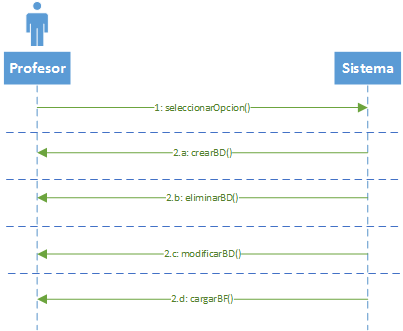
\includegraphics[width=10cm]{imagenes/secuencia_gestionar_bd.png}
\caption{Diagrama de Secuencia - Gestionar BD.}
\label{fig:secgestionarbd}
\end{figure}

\begin{figure}[h!]
\centering
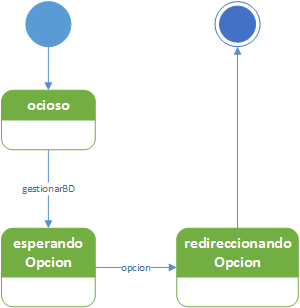
\includegraphics[width=7cm]{imagenes/estado_gestionar_bd.png}
\caption{Diagrama de Estados - Gestionar BD.}
\label{fig:estgestionarbd}
\end{figure}

% Crear BD
\clearpage
\begin{table}[h!]
\footnotesize
\centering
\begin{tabular}{|p{7.5cm}|p{7.5cm}|}
\hline
\rowcolor[HTML]{C0C0C0} 
\textbf{Secci�n Crear BD}                                 & \textbf{ID: CU09}                                                                                                                                                                                                             \\ \hline
\rowcolor[HTML]{EFEFEF} 
\textbf{Curso Normal (Usuario)}                           & \textbf{Curso Normal (Sistema)}                                                                                                                                                                                               \\ \hline
1. El usuario selecciona la opci�n Crear BD               &                                                                                                                                                                                                                               \\ \hline
2. El usuario ingresa los datos de la nueva base de datos &                                                                                                                                                                                                                               \\ \hline
                                                          & 3. El sistema valida los datos y genera una nueva base de datos vac�a, luego redirecciona al men� Gestionar BD (ver Tabla \ref{tab:cugestionarbd})                                                                                            \\ \hline
\rowcolor[HTML]{EFEFEF} 
\textbf{Curso Alternativo (Usuario)}                      & \textbf{Curso Alternativo (Sistema)}                                                                                                                                                                                          \\ \hline
                                                          & Paso 3: Si los datos ingresados no son los correctos o inv�lidos, o no puede generar la nueva base de datos, el sistema indica dicho acontecimiento y vuelve al paso 1. Si el sistema no puede redireccionar, muestra un mensaje de error \\ \hline
\end{tabular}
\caption{Caso de Uso Extendido - Crear BD.}
\label{tab:cucrearbd}
\end{table}

\begin{figure}[h!]
\centering
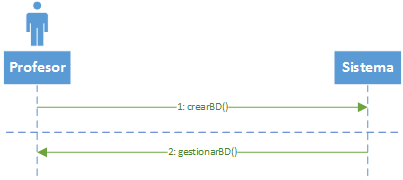
\includegraphics[width=10cm]{imagenes/secuencia_crear_bd.png}
\caption{Diagrama de Secuencia - Crear BD.}
\label{fig:seccrearbd}
\end{figure}

\begin{figure}[h!]
\centering
\includegraphics[width=15cm]{imagenes/estado_crear_bd.png}
\caption{Diagrama de Estados - Crear BD.}
\label{fig:estcrearbd}
\end{figure}

% Eliminar BD
\clearpage
\begin{table}[h!]
\footnotesize
\centering
\begin{tabular}{|p{7.5cm}|p{7.5cm}|}
\hline
\rowcolor[HTML]{C0C0C0} 
\textbf{Secci�n Eliminar BD}                                                                 & \textbf{ID: CU10}                                                                                                                                                                                                             \\ \hline
\rowcolor[HTML]{EFEFEF} 
\textbf{Curso Normal (Usuario)}                                                              & \textbf{Curso Normal (Sistema)}                                                                                                                                                                                               \\ \hline
1. El usuario selecciona la opci�n Eliminar BD                                               &                                                                                                                                                                                                                               \\ \hline
2. El usuario selecciona la base de datos a eliminar                                         &                                                                                                                                                                                                                               \\ \hline
                                                                                             & 3. El sistema solicita la confirmaci�n de la eliminaci�n                                                                                                                                                                      \\ \hline
4. El usuario confirma y acepta la eliminaci�n                                               &                                                                                                                                                                                                                               \\ \hline
                                                                                             & 5. El sistema elimina la base de datos seleccionada                                                                                                                                                                           \\ \hline
                                                                                             & 6. El sistema muestra un mensaje al usuario indicando que ha eliminado la base de datos y redirecciona al men� Gestionar BD (ver Tabla \ref{tab:cugestionarbd})                                                                                  \\ \hline
\rowcolor[HTML]{EFEFEF} 
\textbf{Curso Alternativo (Usuario)}                                                         & \textbf{Curso Alternativo (Sistema)}                                                                                                                                                                                          \\ \hline
Paso 4: El usuario no acepta la confirmaci�n, se termina dicho proceso y se vuelve al paso 1 &                                                                                                                                                                                                                               \\ \hline
                                                                                             & Paso 5: Si el sistema no logra eliminar la base de datos, indica dicho acontecimiento y vuelve al paso 1                                                                                                                      \\ \hline
                                                                                             & Paso 6: Si el sistema no logra redireccionar, manda un mensaje de error                                                                                                                                                       \\ \hline
\end{tabular}
\caption{Caso de Uso Extendido - Eliminar BD.}
\label{tab:cueliminarbd}
\end{table}

\begin{figure}[h!]
\centering
\includegraphics[width=10cm]{imagenes/secuencia_eliminar_bd.png}
\caption{Diagrama de Secuencia - Eliminar BD.}
\label{fig:seceliminarbd}
\end{figure}

\begin{figure}[h!]
\centering
\includegraphics[width=15cm]{imagenes/estado_eliminar_bd.png}
\caption{Diagrama de Estados - Eliminar BD.}
\label{fig:esteliminarbd}
\end{figure}

% Modificar BD
\clearpage
\begin{table}[h!]
\footnotesize
\centering
\begin{tabular}{|p{7.5cm}|p{7.5cm}|}
\hline
\rowcolor[HTML]{C0C0C0} 
\textbf{Secci�n Modificar BD}                                                                & \textbf{ID: CU11}                                                                                                                                 \\ \hline
\rowcolor[HTML]{EFEFEF} 
\textbf{Curso Normal (Usuario)}                                                              & \textbf{Curso Normal (Sistema)}                                                                                                                   \\ \hline
1. El usuario selecciona la opci�n Modificar BD                                              &                                                                                                                                                   \\ \hline
2. El usuario selecciona la base de datos a modificar                                        &                                                                                                                                                   \\ \hline
                                                                                             & 3. El sistema muestra por pantalla los datos de la base de datos seleccionada                                                                     \\ \hline
4. El usuario modifica los campos de dicha base de datos y acepta los cambios                &                                                                                                                                                   \\ \hline
                                                                                             & 5. El sistema valida los nuevos datos y solicita confirmaci�n para ejecutar la modificaci�n                                                       \\ \hline
6. El usuario confirma y acepta la modificaci�n                                              &                                                                                                                                                   \\ \hline
                                                                                             & 7. El sistema modifica la base de datos seleccionada                                                                                              \\ \hline
                                                                                             & 8. El sistema manda un mensaje al usuario indicando que se ha modificado la base de datos y redirecciona al men� Gestionar BD (ver Tabla \ref{tab:cugestionarbd}) \\ \hline
\rowcolor[HTML]{EFEFEF} 
\textbf{Curso Alternativo (Usuario)}                                                         & \textbf{Curso Alternativo (Sistema)}                                                                                                              \\ \hline
                                                                                             & Paso 5: Si los datos ingresados no son los correctos, el sistema indica dicho acontecimiento y vuelve al paso 1                                   \\ \hline
Paso 6: El usuario no acepta la confirmaci�n, se termina dicho proceso y se vuelve al paso 1 &                                                                                                                                                   \\ \hline
                                                                                             & Paso 7: Si el sistema no logra modificar la base de datos, indica dicho acontecimiento y vuelve al paso 1                                         \\ \hline
                                                                                             & Paso 8: Si el sistema no logra redireccionar, manda un mensaje de error                                                                           \\ \hline
\end{tabular}
\caption{Caso de Uso Extendido - Modificar BD.}
\label{tab:cumodificarbd}
\end{table}

\begin{figure}[h!]
\centering
\includegraphics[width=10cm]{imagenes/secuencia_modificar_bd.png}
\caption{Diagrama de Secuencia - Modificar BD.}
\label{fig:secmodificarbd}
\end{figure}

\begin{figure}[h!]
\centering
\includegraphics[width=15cm]{imagenes/estado_modificar_bd.png}
\caption{Diagrama de Estados - Modificar BD.}
\label{fig:estmodificarbd}
\end{figure}

%% Guardar BD
%\clearpage
%\begin{table}[h!]
%\footnotesize
%\centering
%\begin{tabular}{|p{7.5cm}|p{7.5cm}|}
%\hline
%\rowcolor[HTML]{C0C0C0} 
%\textbf{Secci�n Guardar BD}                         & \textbf{ID: CU12}                                                                                                                                                     \\ \hline
%\rowcolor[HTML]{EFEFEF} 
%\textbf{Curso Normal (Usuario)}                     & \textbf{Curso Normal (Sistema)}                                                                                                                                       \\ \hline
%1. El usuario selecciona la opci�n Guardar BD       &                                                                                                                                                                       \\ \hline
%2. El usuario selecciona la base de datos a guardar &                                                                                                                                                                       \\ \hline
%                                                    & 3. El sistema manda un mensaje al usuario indicando que se ha guardado la base de datos y redirecciona al men� Gestionar BD (ver Tabla \ref{tab:cugestionarbd})                       \\ \hline
%\rowcolor[HTML]{EFEFEF} 
%\textbf{Curso Alternativo (Usuario)}                & \textbf{Curso Alternativo (Sistema)}                                                                                                                                  \\ \hline
%                                                    & Paso 3: Si el sistema no logra guardar la base de datos, env�a un mensaje de error y vuelve al paso 1.Si el sistema no logra redireccionar, manda un mensaje de error \\ \hline
%\end{tabular}
%\caption{Caso de Uso Extendido - Guardar BD.}
%\label{tab:cuguardarbd}
%\end{table}
%
%\begin{figure}[h!]
%\centering
%\includegraphics[width=10cm]{imagenes/secuencia_guardar_bd.png}
%\caption{Diagrama de Secuencia - Guardar BD.}
%\label{fig:secguardarbd}
%\end{figure}
%
%\begin{figure}[h!]
%\centering
%\includegraphics[width=12cm]{imagenes/estado_guardar_bd.png}
%\caption{Diagrama de Estados - Guardar BD.}
%\label{fig:estguardarbd}
%\end{figure}

% Cargar BD
\clearpage
\begin{table}[h!]
\footnotesize
\centering
\begin{tabular}{|p{7.5cm}|p{7.5cm}|}
\hline
\rowcolor[HTML]{C0C0C0} 
\textbf{Secci�n Cargar BD}                                 & \textbf{ID: CU12}                                                                                                                                                             \\ \hline
\rowcolor[HTML]{EFEFEF} 
\textbf{Curso Normal (Usuario)}                            & \textbf{Curso Normal (Sistema)}                                                                                                                                               \\ \hline
1. El usuario selecciona la opci�n Cargar BD               &                                                                                                                                                                               \\ \hline
2. El usuario selecciona la base de datos que desea cargar &                                                                                                                                                                               \\ \hline
                                                           & 3. El sistema carga la base de datos seleccionada, muestra un mensaje confirmando la carga y redirecciona al men� Gestionar BD (ver Tabla \ref{tab:cugestionarbd})                            \\ \hline
\rowcolor[HTML]{EFEFEF} 
\textbf{Curso Alternativo (Usuario)}                       & \textbf{Curso Alternativo (Sistema)}                                                                                                                                          \\ \hline
                                                           & Paso 3: Si no puede cargar la base de datos, el sistema indica dicho acontecimiento y vuelve al paso 1. Si el sistema no puede redireccionar, muestra un mensaje de error \\ \hline
\end{tabular}
\caption{Caso de Uso Extendido - Cargar BD.}
\label{tab:cucargarbd}
\end{table}

\begin{figure}[h!]
\centering
\includegraphics[width=10cm]{imagenes/secuencia_cargar_bd.png}
\caption{Diagrama de Secuencia - Cargar BD.}
\label{fig:seccargarbd}
\end{figure}

\begin{figure}[h!]
\centering
\includegraphics[width=12cm]{imagenes/estado_cargar_bd.png}
\caption{Diagrama de Estados - Cargar BD.}
\label{fig:estcargarbd}
\end{figure}

% Gestionar Ejercicios
\clearpage
\begin{table}[h!]
\footnotesize
\centering
\begin{tabular}{|p{7.5cm}|p{7.5cm}|}
\hline
\rowcolor[HTML]{C0C0C0} 
\textbf{Caso de Uso}                                                                                                                                                                                               & \textbf{ID: CU13}                                                                                                                                  \\ \hline
\textbf{Nombre}                                                                                                                                                                                                    & Gestionar Ejercicios                                                                                                                               \\ \hline
\textbf{Actores}                                                                                                                                                                                                   & Profesor                                                                                                                                           \\ \hline
\textbf{Prop�sito}                                                                                                                                                                                                 & Mostrar al Profesor todas las opciones de Gesti�n de Ejercicios: Crear Ejercicios, Eliminar Ejercicios, Modificar Ejercicios, Responder Ejercicios \\ \hline
\textbf{Resumen}                                                                                                                                                                                                   & El Profesor elige una opci�n que se muestra en el men� de gesti�n de ejercicios                                                                    \\ \hline
\rowcolor[HTML]{EFEFEF} 
\textbf{Curso Normal (Usuario)}                                                                                                                                                                                    & \textbf{Curso Normal (Sistema)}                                                                                                                    \\ \hline
1. El profesor ingresa al men� Gestionar Ejercicios desde el Caso de Uso \ref{tab:cugestionarbd} Gestionar BD                                                                                                                            &                                                                                                                                                    \\ \hline
2. El profesor selecciona alguna opci�n: a. Crear Ejercicios (ver Tabla \ref{tab:cucrearejercicios}); b. Eliminar Ejercicios (ver Tabla \ref{tab:cueliminarejercicios}); c. Modificar Ejercicios (ver Tabla \ref{tab:cumodificarejercicios}); d. Responder Ejercicios (ver Tabla \ref{tab:curesponderejercicios}) &                                                                                                                                                    \\ \hline
                                                                                                                                                                                                                   & 3. El sistema direcciona a la opci�n correspondiente                                                                                              \\ \hline
\rowcolor[HTML]{EFEFEF} 
\textbf{Curso Alternativo (Usuario)}                                                                                                                                                                               & \textbf{Curso Alternativo (Sistema)}                                                                                                               \\ \hline
                                                                                                                                                                                                                   & Paso 3: si no se puede direccionar, se muestra un error                                                                                           \\ \hline
\end{tabular}
\caption{Caso de Uso Extendido - Gestionar Ejercicios.}
\label{tab:cugestionarejercicios}
\end{table}

\begin{figure}[h!]
\centering
\includegraphics[width=10cm]{imagenes/secuencia_gestionar_ejercicios.png}
\caption{Diagrama de Secuencia - Gestionar Ejercicios.}
\label{fig:secgestionarejercicios}
\end{figure}

\begin{figure}[h!]
\centering
\includegraphics[width=7cm]{imagenes/estado_gestionar_ejercicios.png}
\caption{Diagrama de Estados - Gestionar Ejercicios.}
\label{fig:estgestionarejercicios}
\end{figure}

% Crear Ejercicios
\clearpage
\begin{table}[h!]
\footnotesize
\centering
\begin{tabular}{|p{7.5cm}|p{7.5cm}|}
\hline
\rowcolor[HTML]{C0C0C0} 
\textbf{Secci�n Crear Ejercicios}                                                                                     & \textbf{ID: CU14}                                                                                                                                                                                                             \\ \hline
\rowcolor[HTML]{EFEFEF} 
\textbf{Curso Normal (Usuario)}                                                                                       & \textbf{Curso Normal (Sistema)}                                                                                                                                                                                               \\ \hline
1. El usuario selecciona la opci�n Crear Ejercicios                                                             &                                                                                                                                                                                                                               \\ \hline
2. El usuario ingresa los datos de los nuevos ejercicios, agregando para cada uno la pregunta y la respuesta esperada &                                                                                                                                                                                                                               \\ \hline
                                                                                                                      & 3. El sistema valida los datos y genera una nueva lista de ejercicios, luego redirecciona al men� Gestionar Ejercicios (ver Tabla \ref{tab:cugestionarejercicios})                                                                                    \\ \hline
\rowcolor[HTML]{EFEFEF} 
\textbf{Curso Alternativo (Usuario)}                                                                                  & \textbf{Curso Alternativo (Sistema)}                                                                                                                                                                                          \\ \hline
                                                                                                                      & Paso 3: Si los datos ingresados no son los correctos, o no puede generar la nueva base de datos, el sistema indica dicho acontecimiento y vuelve al paso 1. Si el sistema no puede redireccionar, muestra un mensaje de error \\ \hline
\end{tabular}
\caption{Caso de Uso Extendido - Crear Ejercicios.}
\label{tab:cucrearejercicios}
\end{table}

\begin{figure}[h!]
\centering
\includegraphics[width=10cm]{imagenes/secuencia_crear_ejercicios.png}
\caption{Diagrama de Secuencia - Crear Ejercicios.}
\label{fig:seccrearejercicios}
\end{figure}

\begin{figure}[h!]
\centering
\includegraphics[width=7cm]{imagenes/estado_crear_ejercicios.png}
\caption{Diagrama de Estados - Crear Ejercicios.}
\label{fig:estcrearejercicios}
\end{figure}

% Eliminar Ejercicios
\clearpage
\begin{table}[h!]
\footnotesize
\centering
\begin{tabular}{|p{7.5cm}|p{7.5cm}|}
\hline
\rowcolor[HTML]{C0C0C0} 
\textbf{Secci�n Eliminar Ejercicios}                                                         & \textbf{ID: CU15}                                                                                                                                       \\ \hline
\rowcolor[HTML]{EFEFEF} 
\textbf{Curso Normal (Usuario)}                                                              & \textbf{Curso Normal (Sistema)}                                                                                                                         \\ \hline
1. El usuario selecciona la opci�n Eliminar Ejercicios                                       &                                                                                                                                                         \\ \hline
2. El usuario selecciona los ejercicios que desea eliminar                                   &                                                                                                                                                         \\ \hline
                                                                                             & 3. El sistema solicita la confirmaci�n de la eliminaci�n                                                                                                \\ \hline
4. El usuario confirma y acepta la eliminaci�n                                               &                                                                                                                                                         \\ \hline
                                                                                             & 5. El sistema elimina los ejercicios seleccionados                                                                                                      \\ \hline
                                                                                             & 6. El sistema muestra un mensaje al usuario indicando que ha eliminado los ejercicios y redirecciona al men� Gestionar Ejercicios (ver Tabla \ref{tab:cugestionarejercicios}) \\ \hline
\rowcolor[HTML]{EFEFEF} 
\textbf{Curso Alternativo (Usuario)}                                                         & \textbf{Curso Alternativo (Sistema)}                                                                                                                    \\ \hline
Paso 4: El usuario no acepta la confirmaci�n, se termina dicho proceso y se vuelve al paso 1 &                                                                                                                                                         \\ \hline
                                                                                             & Paso 5: Si el sistema no logra eliminar los ejercicios, indica dicho acontecimiento y vuelve al paso 1                                                  \\ \hline
                                                                                             & Paso 6: Si el sistema no logra redireccionar, manda un mensaje de error                                                                                 \\ \hline
\end{tabular}
\caption{Caso de Uso Extendido - Eliminar Ejercicios.}
\label{tab:cueliminarejercicios}
\end{table}

\begin{figure}[h!]
\centering
\includegraphics[width=10cm]{imagenes/secuencia_eliminar_ejercicios.png}
\caption{Diagrama de Secuencia - Eliminar Ejercicios.}
\label{fig:seceliminarejercicios}
\end{figure}

\begin{figure}[h!]
\centering
\includegraphics[width=15cm]{imagenes/estado_eliminar_ejercicios.png}
\caption{Diagrama de Estados - Eliminar Ejercicios.}
\label{fig:esteliminarejercicios}
\end{figure}

% Modificar Ejercicios
\clearpage
\begin{table}[h!]
\footnotesize
\centering
\begin{tabular}{|p{7.5cm}|p{7.5cm}|}
\hline
\rowcolor[HTML]{C0C0C0} 
\textbf{Secci�n Modificar Ejercicios}                                                        & \textbf{ID: CU16}                                                                                                                                       \\ \hline
\rowcolor[HTML]{EFEFEF} 
\textbf{Curso Normal (Usuario)}                                                              & \textbf{Curso Normal (Sistema)}                                                                                                                         \\ \hline
1. El usuario selecciona la opci�n Modificar Ejercicios                                      &                                                                                                                                                         \\ \hline
2. El usuario selecciona los ejercicios a modificar                                          &                                                                                                                                                         \\ \hline
                                                                                             & 3. El sistema muestra por pantalla los ejercicios selecionados                                                                                          \\ \hline
4. El usuario modifica los campos de cada ejercicio y acepta los cambios                     &                                                                                                                                                         \\ \hline
                                                                                             & 5. El sistema valida los nuevos ejercicios y solicita confirmaci�n para ejecutar la modificaci�n                                                        \\ \hline
6. El usuario confirma y acepta la modificaci�n                                              &                                                                                                                                                         \\ \hline
                                                                                             & 7. El sistema modifica los ejercicios seleccionados                                                                                                     \\ \hline
                                                                                             & 8. El sistema manda un mensaje al usuario indicando que se ha modificado los ejercicios y redirecciona al men� Gestionar Ejercicios (ver Tabla \ref{tab:cugestionarejercicios}) \\ \hline
\rowcolor[HTML]{EFEFEF} 
\textbf{Curso Alternativo (Usuario)}                                                         & \textbf{Curso Alternativo (Sistema)}                                                                                                                    \\ \hline
                                                                                             & Paso 5: Si los datos ingresados no son los correctos, el sistema indica dicho acontecimiento y vuelve al paso 1                                         \\ \hline
Paso 6: El usuario no acepta la confirmaci�n, se termina dicho proceso y se vuelve al paso 1 &                                                                                                                                                         \\ \hline
                                                                                             & Paso 7: Si el sistema no logra modificar los ejercicios, indica dicho acontecimiento y vuelve al paso 1                                                 \\ \hline
                                                                                             & Paso 8: Si el sistema no logra redireccionar, manda un mensaje de error                                                                                 \\ \hline
\end{tabular}
\caption{Caso de Uso Extendido - Modificar Ejercicios.}
\label{tab:cumodificarejercicios}
\end{table}

\begin{figure}[h!]
\centering
\includegraphics[width=10cm]{imagenes/secuencia_modificar_ejercicios.png}
\caption{Diagrama de Secuencia - Modificar Ejercicios.}
\label{fig:secmodificarejercicios}
\end{figure}

\begin{figure}[h!]
\centering
\includegraphics[width=15cm]{imagenes/estado_modificar_ejercicios.png}
\caption{Diagrama de Estados - Modificar Ejercicios.}
\label{fig:estmodificarejercicios}
\end{figure}

% Responder Ejercicios
\clearpage
\begin{table}[h!]
\footnotesize
\centering
\begin{tabular}{|p{7.5cm}|p{7.5cm}|}
\hline
\rowcolor[HTML]{C0C0C0} 
\textbf{Secci�n Responder Ejercicios}                                                                               & \textbf{ID: CU17}                                                                                                                                                                                                                                                    \\ \hline
\rowcolor[HTML]{EFEFEF} 
\textbf{Curso Normal (Usuario)}                                                                                     & \textbf{Curso Normal (Sistema)}                                                                                                                                                                                                                                      \\ \hline
1. El usuario selecciona la opci�n Responder Ejercicios                                                             &                                                                                                                                                                                                                                                                      \\ \hline
2. El usuario responde el ejercicio que sale en pantalla v�a una consulta en �lgebra Relacional (ver Tabla \ref{tab:cuhacerconsulta}) &                                                                                                                                                                                                                                                                      \\ \hline
                                                                                                                    & 3. El sistema verifica la sintaxis y sem�ntica de la respuesta, ejecuta la consulta y compara con la respuesta esperada                                                                                                                                             \\ \hline
                                                                                                                    & 4. El sistema muestra el resultado de la consulta y carga la siguiente consulta volviendo al paso 2, hasta que ya no hay m�s ejercicios                                                                                                                             \\ \hline
                                                                                                                    & 5. Cuando no hay m�s ejercicios, el sistema muestra el resultado global de todos los ejercicios y redirecciona a: men� Gestionar Ejercicios si el usuario es un Profesor (ver Tabla \ref{tab:cugestionarejercicios}), o al men� Sesi�n Alumno si el usuario es un Alumno (ver Tabla \ref{tab:cusesionalumno}) \\ \hline
\rowcolor[HTML]{EFEFEF} 
\textbf{Curso Alternativo (Usuario)}                                                                                & \textbf{Curso Alternativo (Sistema)}                                                                                                                                                                                                                                 \\ \hline
                                                                                                                    & Paso 3: Si el sistema encuentra un error de sintaxis o sem�ntica, muestra un mensaje de error y vuelve al paso 2. Si el sistema no logra ejecutar la respuesta, muestra un mensaje de error y vuelve al paso 2                                                       \\ \hline
                                                                                                                    & Paso 4: Si el sistema no logra cargar la siguiente pregunta, muestra un mensaje de error y vuelve al paso 1                                                                                                                                                          \\ \hline
                                                                                                                    & Paso 5: Si el sistema no logra redireccionar, se muestra un mensaje de error                                                                                                                                                                                         \\ \hline
\end{tabular}
\caption{Caso de Uso Extendido - Responder Ejercicios.}
\label{tab:curesponderejercicios}
\end{table}

\begin{figure}[h!]
\centering
\includegraphics[width=10cm]{imagenes/secuencia_responder_ejercicios.png}
\caption{Diagrama de Secuencia - Responder Ejercicios.}
\label{fig:secresponderejercicios}
\end{figure}

\begin{figure}[h!]
\centering
\includegraphics[width=15cm]{imagenes/estado_responder_ejercicios.png}
\caption{Diagrama de Estados - Responder Ejercicios.}
\label{fig:estresponderejercicios}
\end{figure}

% Gestionar Relaci�n
\clearpage
\begin{table}[h!]
\footnotesize
\centering
\begin{tabular}{|p{7.5cm}|p{7.5cm}|}
\hline
\rowcolor[HTML]{C0C0C0} 
\textbf{Caso de Uso}                                                                                                                                                                                      & \textbf{ID: CU18}                                                                                                                   \\ \hline
\textbf{Nombre}                                                                                                                                                                                           & Gestionar Relaci�n                                                                                                                  \\ \hline
\textbf{Actores}                                                                                                                                                                                          & Usuario (Alumno, Profesor)                                                                                                          \\ \hline
\textbf{Prop�sito}                                                                                                                                                                                        & Mostrar al Usuario todas las opciones de Gesti�n de Relaci�n: Agregar Relaci�n, Eliminar Relaci�n, Modificar Relaci�n, Ver Relaci�n \\ \hline
\textbf{Resumen}                                                                                                                                                                                          & El Usuario elige una opci�n que se muestra en el men� de gesti�n de relaciones                                                      \\ \hline
\rowcolor[HTML]{EFEFEF} 
\textbf{Curso Normal (Usuario)}                                                                                                                                                                           & \textbf{Curso Normal (Sistema)}                                                                                                     \\ \hline
1. El usuario ingresa al men� Gestionar Relaci�n desde el men� Gestionar BD si es un profesor (ver Tabla \ref{tab:cugestionarbd}) o desde el men� Sesi�n Alumno si es un alumno (ver Tabla \ref{tab:cusesionalumno})                    &                                                                                                                                     \\ \hline
2. El usuario selecciona alguna opci�n: a. Agregar Relaci�n (ver Tabla \ref{tab:cuagregarrelacion}); b. Eliminar Relaci�n (ver Tabla \ref{tab:cueliminarrelacion}); c. Modificar Relaci�n (ver Tabla \ref{tab:cumodificarrelacion}); d. Ver Relaci�n (ver Tabla \ref{tab:cuverrelacion}) &                                                                                                                                     \\ \hline
                                                                                                                                                                                                          & 3. El sistema direcciona a la opci�n correspondiente                                                                             \\ \hline
\rowcolor[HTML]{EFEFEF} 
\textbf{Curso Alternativo (Usuario)}                                                                                                                                                                      & \textbf{Curso Alternativo (Sistema)}                                                                                                \\ \hline
                                                                                                                                                                                                          & Paso 3: si no se puede direccionar, se muestra un error                                                                           \\ \hline
\end{tabular}
\caption{Caso de Uso Extendido - Gestionar Relaci�n.}
\label{tab:cugestionarrelacion}
\end{table}

\begin{figure}[h!]
\centering
\includegraphics[width=10cm]{imagenes/secuencia_gestionar_relacion.png}
\caption{Diagrama de Secuencia - Gestionar Relaci�n.}
\label{fig:secgestionarrelacion}
\end{figure}

\begin{figure}[h!]
\centering
\includegraphics[width=7cm]{imagenes/estado_gestionar_relacion.png}
\caption{Diagrama de Estados - Gestionar Relaci�n.}
\label{fig:estgestionarrelacion}
\end{figure}

% Agregar Relaci�n
\clearpage
\begin{table}[h!]
\footnotesize
\centering
\begin{tabular}{|p{7.5cm}|p{7.5cm}|}
\hline
\rowcolor[HTML]{C0C0C0} 
\textbf{Secci�n Agregar Relaci�n}                    & \textbf{ID: CU19}                                                                                                                                                                                                                   \\ \hline
\rowcolor[HTML]{EFEFEF} 
\textbf{Curso Normal (Usuario)}                      & \textbf{Curso Normal (Sistema)}                                                                                                                                                                                                     \\ \hline
1. El usuario selecciona la opci�n Agregar Relaci�n  &                                                                                                                                                                                                                                     \\ \hline
2. El usuario ingresa los datos de la nueva relaci�n &                                                                                                                                                                                                                                     \\ \hline
                                                     & 3. El sistema valida los datos y genera una nueva relaci�n, luego redirecciona al men� Gestionar Relaci�n (ver Tabla \ref{tab:cugestionarrelacion})                                                                                                       \\ \hline
\rowcolor[HTML]{EFEFEF} 
\textbf{Curso Alternativo (Usuario)}                 & \textbf{Curso Alternativo (Sistema)}                                                                                                                                                                                                \\ \hline
                                                     & Paso 3: Si no puede generar la nueva relaci�n, el sistema indica dicho acontecimiento y vuelve al paso 1. Si el sistema no puede redireccionar, muestra un mensaje de error \\ \hline
\end{tabular}
\caption{Caso de Uso Extendido - Agregar Relaci�n.}
\label{tab:cuagregarrelacion}
\end{table}

\begin{figure}[h!]
\centering
\includegraphics[width=10cm]{imagenes/secuencia_agregar_relacion.png}
\caption{Diagrama de Secuencia - Agregar Relaci�n.}
\label{fig:secagregarrelacion}
\end{figure}

\begin{figure}[h!]
\centering
\includegraphics[width=12cm]{imagenes/estado_agregar_relacion.png}
\caption{Diagrama de Estados - Agregar Relaci�n.}
\label{fig:estagregarrelacion}
\end{figure}

% Eliminar Relaci�n
\clearpage
\begin{table}[h!]
\footnotesize
\centering
\begin{tabular}{|p{7.5cm}|p{7.5cm}|}
\hline
\rowcolor[HTML]{C0C0C0} 
\textbf{Secci�n Eliminar Relaci�n}                                                           & \textbf{ID: CU20}                                                                                                                                \\ \hline
\rowcolor[HTML]{EFEFEF} 
\textbf{Curso Normal (Usuario)}                                                              & \textbf{Curso Normal (Sistema)}                                                                                                                  \\ \hline
1. El usuario selecciona la opci�n Eliminar Relaci�n                                         &                                                                                                                                                  \\ \hline
2. El usuario selecciona la relaci�n que desea eliminar                                      &                                                                                                                                                  \\ \hline
                                                                                             & 3. El sistema solicita la confirmaci�n de la eliminaci�n                                                                                         \\ \hline
4. El usuario confirma y acepta la eliminaci�n                                               &                                                                                                                                                  \\ \hline
                                                                                             & 5. El sistema elimina la relaci�n seleccionada                                                                                                   \\ \hline
                                                                                             & 6. El sistema muestra un mensaje al usuario indicando que ha eliminado la relaci�n y redirecciona al men� Gestionar Relaci�n (ver Tabla \ref{tab:cugestionarrelacion}) \\ \hline
\rowcolor[HTML]{EFEFEF} 
\textbf{Curso Alternativo (Usuario)}                                                         & \textbf{Curso Alternativo (Sistema)}                                                                                                             \\ \hline
Paso 4: El usuario no acepta la confirmaci�n, se termina dicho proceso y se vuelve al paso 1 &                                                                                                                                                  \\ \hline
                                                                                             & Paso 5: Si el sistema no logra eliminar la relaci�n, indica dicho acontecimiento y vuelve al paso 1                                              \\ \hline
                                                                                             & Paso 6: Si el sistema no logra redireccionar, manda un mensaje de error                                                                          \\ \hline
\end{tabular}
\caption{Caso de Uso Extendido - Eliminar Relaci�n.}
\label{tab:cueliminarrelacion}
\end{table}

\begin{figure}[h!]
\centering
\includegraphics[width=10cm]{imagenes/secuencia_eliminar_relacion.png}
\caption{Diagrama de Secuencia - Eliminar Relaci�n.}
\label{fig:seceliminarrelacion}
\end{figure}

\begin{figure}[h!]
\centering
\includegraphics[width=15cm]{imagenes/estado_eliminar_relacion.png}
\caption{Diagrama de Estados - Eliminar Relaci�n.}
\label{fig:esteliminarrelacion}
\end{figure}

% Modificar Relaci�n
\clearpage
\begin{table}[h!]
\footnotesize
\centering
\begin{tabular}{|p{7.5cm}|p{7.5cm}|}
\hline
\rowcolor[HTML]{C0C0C0} 
\textbf{Secci�n Modificar Relaci�n}                                                          & \textbf{ID: CU21}                                                                                                                                  \\ \hline
\rowcolor[HTML]{EFEFEF} 
\textbf{Curso Normal (Usuario)}                                                              & \textbf{Curso Normal (Sistema)}                                                                                                                    \\ \hline
1. El usuario selecciona la opci�n Modificar Relaci�n                                        &                                                                                                                                                    \\ \hline
2. El usuario selecciona la relaci�n a modificar                                             &                                                                                                                                                    \\ \hline
                                                                                             & 3. El sistema muestra por pantalla la relaci�n seleccionada                                                                                        \\ \hline
4. El usuario modifica los campos de la relaci�n                                             &                                                                                                                                                    \\ \hline
                                                                                             & 5. El sistema valida los nuevos campos de la relaci�n y solicita confirmaci�n para ejecutar la modificaci�n                                        \\ \hline
6. El usuario confirma y acepta la modificaci�n                                              &                                                                                                                                                    \\ \hline
                                                                                             & 7. El sistema modifica la relaci�n seleccionada                                                                                                    \\ \hline
                                                                                             & 8. El sistema manda un mensaje al usuario indicando que se ha modificado la relaci�n y redirecciona al men� Gestionar Relaci�n (ver Tabla \ref{tab:cugestionarrelacion}) \\ \hline
\rowcolor[HTML]{EFEFEF} 
\textbf{Curso Alternativo (Usuario)}                                                         & \textbf{Curso Alternativo (Sistema)}                                                                                                               \\ \hline
Paso 6: El usuario no acepta la confirmaci�n, se termina dicho proceso y se vuelve al paso 1 &                                                                                                                                                    \\ \hline
                                                                                             & Paso 7: Si el sistema no logra modificar la relaci�n, indica dicho acontecimiento y vuelve al paso 1                                               \\ \hline
                                                                                             & Paso 8: Si el sistema no logra redireccionar, manda un mensaje de error                                                                            \\ \hline
\end{tabular}
\caption{Caso de Uso Extendido - Modificar Relaci�n}
\label{tab:cumodificarrelacion}
\end{table}

\begin{figure}[h!]
\centering
\includegraphics[width=10cm]{imagenes/secuencia_modificar_relacion.png}
\caption{Diagrama de Secuencia - Modificar Relaci�n.}
\label{fig:secmodificarrelacion}
\end{figure}

\begin{figure}[h!]
\centering
\includegraphics[width=15cm]{imagenes/estado_modificar_relacion.png}
\caption{Diagrama de Estados - Modificar Relaci�n.}
\label{fig:estmodificarrelacion}
\end{figure}

% Ver Relaci�n
\clearpage
\begin{table}[h!]
\footnotesize
\centering
\begin{tabular}{|p{7.5cm}|p{7.5cm}|}
\hline
\rowcolor[HTML]{C0C0C0} 
\textbf{Secci�n Ver Relaci�n}                         & \textbf{ID: CU22}                                                                                                    \\ \hline
\rowcolor[HTML]{EFEFEF} 
\textbf{Curso Normal (Usuario)}                       & \textbf{Curso Normal (Sistema)}                                                                                      \\ \hline
1. El usuario selecciona la opci�n Ver Relaci�n                               &                                                                                                                      \\ \hline
2. El usuario selecciona una relaci�n desde una lista                         &                                                                                                                      \\ \hline
                                                                              & 3. El sistema muestra por pantalla la relaci�n seleccionada                                                          \\ \hline
4. El usuario puede seleccionar la opci�n Gestionar Tupla (ver Tabla \ref{tab:cugestionartupla}) &                                                                                                                      \\ \hline
                                                                              & 5. El sistema direcciona a Gestionar Tupla (ver Tabla \ref{tab:cugestionartupla}) si es que el usuario lo ha decidido                   \\ \hline
\rowcolor[HTML]{EFEFEF} 
\textbf{Curso Alternativo (Usuario)}                                          & \textbf{Curso Alternativo (Sistema)}                                                                                 \\ \hline
                                                                              & Paso 3: Si el sistema no logra cargar la relaci�n seleccionada, se muestra un mensaje de error y se vuelve al paso 1 \\ \hline
                                                                              & Paso 5: Si el sistema no logra direccionar, se muestra un mensaje de error                                           \\ \hline

\end{tabular}
\caption{Caso de Uso Extendido - Ver Relaci�n.}
\label{tab:cuverrelacion}
\end{table}

\begin{figure}[h!]
\centering
\includegraphics[width=10cm]{imagenes/secuencia_ver_relacion.png}
\caption{Diagrama de Secuencia - Ver Relaci�n.}
\label{fig:secverrelacion}
\end{figure}

\begin{figure}[h!]
\centering
\includegraphics[width=10cm]{imagenes/estado_ver_relacion.png}
\caption{Diagrama de Estados - Ver Relaci�n.}
\label{fig:estverrelacion}
\end{figure}

% Gestionar Tuplas
\clearpage
\begin{table}[h!]
\footnotesize
\centering
\begin{tabular}{|p{7.5cm}|p{7.5cm}|}
\hline
\rowcolor[HTML]{C0C0C0} 
\textbf{Caso de Uso}                                                                                                                                        & \textbf{ID: CU23}                                                                                         \\ \hline
\textbf{Nombre}                                                                                                                                             & Gestionar Tupla                                                                                           \\ \hline
\textbf{Actores}                                                                                                                                            & Usuario (Alumno, Profesor)                                                                                \\ \hline
\textbf{Prop�sito}                                                                                                                                          & Mostrar al Usuario todas las opciones de Gesti�n de Tupla: Ingresar Tupla, Eliminar Tupla, Modificar Tupla \\ \hline
\textbf{Resumen}                                                                                                                                            & El Usuario elige una opci�n que se muestra en el men� de gesti�n de tuplas                                \\ \hline
\rowcolor[HTML]{EFEFEF} 
\textbf{Curso Normal (Usuario)}                                                                                                                             & \textbf{Curso Normal (Sistema)}                                                                           \\ \hline
1. El usuario ingresa al men� Gestionar Tupla desde la opci�n Ver Relaci�n (ver Tabla \ref{tab:cuverrelacion})                                                              &                                                                                                           \\ \hline
2. El usuario selecciona alguna opci�n: a. Ingresar Tupla (ver Tabla \ref{tab:cuagregartupla}); b. Eliminar Tupla (ver Tabla \ref{tab:cueliminartupla}); c. Modificar Tupla (ver Tabla \ref{tab:cumodificartupla}) &                                                                                                           \\ \hline
                                                                                                                                                            & 3. El sistema direcciona a la opci�n correspondiente                                                     \\ \hline
\rowcolor[HTML]{EFEFEF} 
\textbf{Curso Alternativo (Usuario)}                                                                                                                        & \textbf{Curso Alternativo (Sistema)}                                                                      \\ \hline
                                                                                                                                                            & Paso 3: si no se puede direccionar, se muestra un error                                                 \\ \hline
\end{tabular}
\caption{Caso de Uso Extendido - Gestionar Tupla.}
\label{tab:cugestionartupla}
\end{table}

\begin{figure}[h!]
\centering
\includegraphics[width=10cm]{imagenes/secuencia_gestionar_tupla.png}
\caption{Diagrama de Secuencia - Gestionar Tupla.}
\label{fig:secgestionartupla}
\end{figure}

\begin{figure}[h!]
\centering
\includegraphics[width=7cm]{imagenes/estado_gestionar_tupla.png}
\caption{Diagrama de Estados - Gestionar Tupla.}
\label{fig:estgestionartupla}
\end{figure}

% Ingresar Tupla
\clearpage
\begin{table}[h!]
\footnotesize
\centering
\begin{tabular}{|p{7.5cm}|p{7.5cm}|}
\hline
\rowcolor[HTML]{C0C0C0} 
\textbf{Secci�n Ingresar Tupla}                    & \textbf{ID: CU24}                                                                                                                                                                                                     \\ \hline
\rowcolor[HTML]{EFEFEF} 
\textbf{Curso Normal (Usuario)}                   & \textbf{Curso Normal (Sistema)}                                                                                                                                                                                       \\ \hline
1. El usuario selecciona la opci�n Ingresar Tupla  &                                                                                                                                                                                                                       \\ \hline
2. El usuario ingresa los datos de la nueva tupla &                                                                                                                                                                                                                       \\ \hline
                                                  & 3. El sistema valida los datos y genera una nueva tupla, luego redirecciona al men� Gestionar Tupla (ver Tabla \ref{tab:cugestionartupla})                                                                                               \\ \hline
\rowcolor[HTML]{EFEFEF} 
\textbf{Curso Alternativo (Usuario)}              & \textbf{Curso Alternativo (Sistema)}                                                                                                                                                                                  \\ \hline
                                                  & Paso 3: Si los tipos datos ingresados no son los correctos, o no puede generar la nueva tupla, el sistema indica dicho acontecimiento y vuelve al paso 1. Si el sistema no puede redireccionar, muestra un mensaje de error \\ \hline
\end{tabular}
\caption{Caso de Uso Extendido - Ingresar Tupla.}
\label{tab:cuagregartupla}
\end{table}

\begin{figure}[h!]
\centering
\includegraphics[width=10cm]{imagenes/secuencia_agregar_tupla.png}
\caption{Diagrama de Secuencia - Ingresar Tupla.}
\label{fig:secagregartupla}
\end{figure}

\begin{figure}[h!]
\centering
\includegraphics[width=12cm]{imagenes/estado_agregar_tupla.png}
\caption{Diagrama de Estados - Ingresar Tupla.}
\label{fig:estagregartupla}
\end{figure}

% Eliminar Tupla
\clearpage
\begin{table}[h!]
\footnotesize
\centering
\begin{tabular}{|p{7.5cm}|p{7.5cm}|}
\hline
\rowcolor[HTML]{C0C0C0} 
\textbf{Secci�n Eliminar Tupla}                                                              & \textbf{ID: CU25}                                                                                                                          \\ \hline
\rowcolor[HTML]{EFEFEF} 
\textbf{Curso Normal (Usuario)}                                                              & \textbf{Curso Normal (Sistema)}                                                                                                            \\ \hline
1. El usuario selecciona la opci�n Eliminar Tupla                                            &                                                                                                                                            \\ \hline
2. El usuario selecciona la tupla que desea eliminar                                         &                                                                                                                                            \\ \hline
                                                                                             & 3. El sistema solicita la confirmaci�n de la eliminaci�n                                                                                   \\ \hline
4. El usuario confirma y acepta la eliminaci�n                                               &                                                                                                                                            \\ \hline
                                                                                             & 5. El sistema elimina la tupla seleccionada                                                                                                \\ \hline
                                                                                             & 6. El sistema muestra un mensaje al usuario indicando que ha eliminado la tupla y redirecciona al men� Gestionar Tupla (ver Tabla \ref{tab:cugestionartupla}) \\ \hline
\rowcolor[HTML]{EFEFEF} 
\textbf{Curso Alternativo (Usuario)}                                                         & \textbf{Curso Alternativo (Sistema)}                                                                                                       \\ \hline
Paso 4: El usuario no acepta la confirmaci�n, se termina dicho proceso y se vuelve al paso 1 &                                                                                                                                            \\ \hline
                                                                                             & Paso 5: Si el sistema no logra eliminar la tupla, indica dicho acontecimiento y vuelve al paso 1                                           \\ \hline
                                                                                             & Paso 6: Si el sistema no logra redireccionar, manda un mensaje de error                                                                    \\ \hline
\end{tabular}
\caption{Caso de Uso Extendido - Eliminar Tupla.}
\label{tab:cueliminartupla}
\end{table}

\begin{figure}[h!]
\centering
\includegraphics[width=10cm]{imagenes/secuencia_eliminar_tupla.png}
\caption{Diagrama de Secuencia - Eliminar Tupla.}
\label{fig:seceliminartupla}
\end{figure}

\begin{figure}[h!]
\centering
\includegraphics[width=15cm]{imagenes/estado_eliminar_tupla.png}
\caption{Diagrama de Estados - Eliminar Tupla.}
\label{fig:esteliminartupla}
\end{figure}

% Modificar Tupla
\clearpage
\begin{table}[h!]
\footnotesize
\centering
\begin{tabular}{|p{7.5cm}|p{7.5cm}|}
\hline
\rowcolor[HTML]{C0C0C0} 
\textbf{Secci�n Modificar Tupla}                                                             & \textbf{ID: CU26}                                                                                                                               \\ \hline
\rowcolor[HTML]{EFEFEF} 
\textbf{Curso Normal (Usuario)}                                                              & \textbf{Curso Normal (Sistema)}                                                                                                                 \\ \hline
1. El usuario selecciona la opci�n Modificar Tupla                                           &                                                                                                                                                 \\ \hline
2. El usuario selecciona la tupla a modificar                                                &                                                                                                                                                 \\ \hline
                                                                                             & 3. El sistema muestra por pantalla la tupla seleccionada                                                                                        \\ \hline
4. El usuario modifica los campos de la tupla                                                &                                                                                                                                                 \\ \hline
                                                                                             & 5. El sistema valida los nuevos campos de la tupla y solicita confirmaci�n para ejecutar la modificaci�n                                        \\ \hline
6. El usuario confirma y acepta la modificaci�n                                              &                                                                                                                                                 \\ \hline
                                                                                             & 7. El sistema modifica la tupla seleccionada                                                                                                    \\ \hline
                                                                                             & 8. El sistema manda un mensaje al usuario indicando que se ha modificado la tupla y redirecciona al men� Gestionar Tupla (ver Tabla \ref{tab:cugestionartupla}) \\ \hline
\rowcolor[HTML]{EFEFEF} 
\textbf{Curso Alternativo (Usuario)}                                                         & \textbf{Curso Alternativo (Sistema)}                                                                                                            \\ \hline
                                                                                             & Paso 5: Si los tipos de datos ingresados no son los correctos, el sistema indica dicho acontecimiento y vuelve al paso 1                                 \\ \hline
Paso 6: El usuario no acepta la confirmaci�n, se termina dicho proceso y se vuelve al paso 1 &                                                                                                                                                 \\ \hline
                                                                                             & Paso 7: Si el sistema no logra modificar la tupla, indica dicho acontecimiento y vuelve al paso 1                                               \\ \hline
                                                                                             & Paso 8: Si el sistema no logra redireccionar, manda un mensaje de error                                                                         \\ \hline
\end{tabular}
\caption{Caso de Uso Extendido - Modificar Tupla.}
\label{tab:cumodificartupla}
\end{table}

\begin{figure}[h!]
\centering
\includegraphics[width=10cm]{imagenes/secuencia_modificar_tupla.png}
\caption{Diagrama de Secuencia - Modificar Tupla.}
\label{fig:secmodificartupla}
\end{figure}

\begin{figure}[h!]
\centering
\includegraphics[width=15cm]{imagenes/estado_modificar_tupla.png}
\caption{Diagrama de Estados - Modificar Tupla.}
\label{fig:estmodificartupla}
\end{figure}

% Sesi�n Alumno
\clearpage
\begin{table}[h!]
\footnotesize
\centering
\begin{tabular}{|p{7.5cm}|p{7.5cm}|}
\hline
\rowcolor[HTML]{C0C0C0} 
\textbf{Caso de Uso}                                                                                                                                                                                    & \textbf{ID: CU27}                                                                                                                                                \\ \hline
\textbf{Nombre}                                                                                                                                                                                         & Sesi�n Alumno                                                                                                                                                    \\ \hline
\textbf{Actores}                                                                                                                                                                                        & Alumno                                                                                                                                                           \\ \hline
\textbf{Prop�sito}                                                                                                                                                                                      & Mostrar al Alumno todas las opciones relacionadas con la Gesti�n de Bases de Datos, Relaciones, Tuplas, Hacer Consultas y Responder Ejercicios \\ \hline
\textbf{Resumen}                                                                                                                                                                                        & El Usuario elige una opci�n que se muestra en el men�: Gesti�n de tuplas, Gestionar Relaci�n, Modificar Cuenta, Gesti�n BD, Responder Ejercicios, Hacer Consulta \\ \hline
\rowcolor[HTML]{EFEFEF} 
\textbf{Curso Normal (Usuario)}                                                                                                                                                                         & \textbf{Curso Normal (Sistema)}                                                                                                                                  \\ \hline
1. El usuario ingresa al sistema desde el Caso de Uso \ref{tab:cuiniciarsesion} Iniciar Sesi�n                                                                                                                                  &                                                                                                                                                                  \\ \hline
2. El usuario selecciona alguna opci�n: a. Crear BD (ver Tabla \ref{tab:cucrearbd}); b. Eliminar BD (ver Tabla \ref{tab:cueliminarbd}); c. Modificar BD (ver Tabla \ref{tab:cumodificarbd}); d. Cargar BD (ver Tabla \ref{tab:cucargarbd}); e. Gestionar Relaciones (ver Tabla \ref{tab:cugestionarrelacion}); f. Responder Ejercicios (ver Tabla \ref{tab:curesponderejercicios}); g. Hacer Consulta (ver Tabla \ref{tab:cuhacerconsulta}); h. Modificar Cuenta (ver Tabla \ref{tab:cumodificarcuenta}) &  \\ \hline
                                                                                                                                                                                                        & 3. El sistema direcciona a la opci�n correspondiente                                                                                                            \\ \hline
\rowcolor[HTML]{EFEFEF} 
\textbf{Curso Alternativo (Usuario)}                                                                                                                                                                    & \textbf{Curso Alternativo (Sistema)}                                                                                                                             \\ \hline
                                                                                                                                                                                                        & Paso 3: si no se puede direccionar, se muestra un error                                                                                                         \\ \hline
\end{tabular}
\caption{Caso de Uso Extendido - Sesi�n Alumno.}
\label{tab:cusesionalumno}
\end{table}

\begin{figure}[h!]
\centering
\includegraphics[width=10cm]{imagenes/secuencia_sesion_alumno.png}
\caption{Diagrama de Secuencia - Sesi�n Alumno}
\label{fig:secsesionalumno}
\end{figure}

\begin{figure}[h!]
\centering
\includegraphics[width=7cm]{imagenes/estado_sesion_alumno.png}
\caption{Diagrama de Estados - Sesi�n Alumno.}
\label{fig:estsesionalumno}
\end{figure}

% Hacer Consulta
\clearpage
\begin{table}[h!]
\footnotesize
\centering
\begin{tabular}{|p{7.5cm}|p{7.5cm}|}
\hline
\rowcolor[HTML]{C0C0C0} 
\textbf{Caso de Uso}                                                                                                                                                                            & \textbf{ID: CU28}                                                                                                                                                                                                                                                        \\ \hline
\textbf{Nombre}                                                                                                                                                                                 & Hacer Consulta                                                                                                                                                                                                                                                           \\ \hline
\textbf{Actores}                                                                                                                                                                                & Usuario (Alumno, Profesor)                                                                                                                                                                                                                                               \\ \hline
\textbf{Prop�sito}                                                                                                                                                                              & Entregar herramientas para la ejecuci�n de consultas en �lgebra Relacional                                                                                                                                                                                               \\ \hline
\textbf{Resumen}                                                                                                                                                                                & El Usuario escribe manualmente o selecciona alg�n bot�n para ejecutar una consulta en �lgebra Relacional                                                                                                                                                                 \\ \hline
\rowcolor[HTML]{EFEFEF} 
\textbf{Curso Normal (Usuario)}                                                                                                                                                                 & \textbf{Curso Normal (Sistema)}                                                                                                                                                                                                                                          \\ \hline
1. El usuario escribe en el campo para hacer consultas desde la Sesi�n Profesor, si es un profesor (ver Tabla \ref{tab:cusesionprofesor}); o desde la Sesi�n Alumno, si es un alumno (ver Tabla \ref{tab:cusesionalumno}) &                                                                                                                                                                                                                                                                          \\ \hline
2. El usuario v�a teclado o por medio de botones gr�ficos, y a base de las relaciones cargadas; formula una consulta en �lgebra Relacional y la ejecuta                                         &                                                                                                                                                                                                                                                                          \\ \hline
                                                                                                                                                                                                & 3. El sistema revisa sintaxis y sem�ntica de la consulta realizada y genera la relaci�n resultante                                                                                                                                                                      \\ \hline
                                                                                                                                                                                                & 4. El sistema permite generar otra consulta si es que el usuario lo desea, volviendo al paso 2                                                                                                                                                                           \\ \hline
\rowcolor[HTML]{EFEFEF} 
\textbf{Curso Alternativo (Usuario)}                                                                                                                                                            & \textbf{Curso Alternativo (Sistema)}                                                                                                                                                                                                                                     \\ \hline
                                                                                                                                                                                                & Paso 3: Si el sistema encuentra un error de sintaxis, no logra revisar la consulta o no puede generar la nueva relaci�n, muestra un aviso de error y vuelve al paso 1                                                                                                                                   \\ \hline
                                                                                                                                                                                                & Paso 4: Si el sistema no puede ofrecer al usuario hacer otra consulta, muestra un mensaje y vuelve al men� Sesi�n Profesor si es que el usuario es un profesor (ver Tabla \ref{tab:cusesionprofesor}), o vuelve al men� Sesi�n Alumno si es que el usuario es un alumno (ver Tabla \ref{tab:cusesionalumno}) \\ \hline
\end{tabular}
\caption{Caso de Uso Extendido - Hacer Consulta.}
\label{tab:cuhacerconsulta}
\end{table}

\begin{figure}[h!]
\centering
\includegraphics[width=10cm]{imagenes/secuencia_hacer_consulta.png}
\caption{Diagrama de Secuencia - Hacer Consulta.}
\label{fig:sechacerconsulta}
\end{figure}

\begin{figure}[h!]
\centering
\includegraphics[width=15cm]{imagenes/estado_hacer_consulta.png}
\caption{Diagrama de Estados - Hacer Consulta.}
\label{fig:esthacerconsulta}
\end{figure}

% Ver Estad�sticas
\clearpage
\begin{table}[h!]
\footnotesize
\centering
\begin{tabular}{|p{7.5cm}|p{7.5cm}|}
\hline
\rowcolor[HTML]{C0C0C0} 
\textbf{Caso de Uso}                                                                                  & \textbf{ID: CU29}                                                                                                                              \\ \hline
\textbf{Nombre}                                                                                       & Ver Estad�sticas                                                                                                                               \\ \hline
\textbf{Actores}                                                                                      & Profesor                                                                                                                                       \\ \hline
\textbf{Prop�sito}                                                                                    & Obtener feedback mediante estad�sticas y datos de todos los alumnos que han utilizado la herramienta                                           \\ \hline
\textbf{Resumen}                                                                                      & El Profesor observa tablas y resultados obtenidos por alg�n algoritmo de Miner�a de Datos                                                      \\ \hline
\rowcolor[HTML]{EFEFEF} 
\textbf{Curso Normal (Usuario)}                                                                       & \textbf{Curso Normal (Sistema)}                                                                                                                \\ \hline
1. El usuario selecciona la opci�n Ver Estad�sticas desde el men� Sesi�n Profesor (ver Tabla \ref{tab:cusesionprofesor}) &                                                                                                                                                \\ \hline
                                                                                                      & 2. El sistema muestra estad�sticas de la base de datos, adem�s de un gr�fico de resultado de ejercicios                              \\ \hline
\rowcolor[HTML]{EFEFEF} 
\textbf{Curso Alternativo (Usuario)}                                                                  & \textbf{Curso Alternativo (Sistema)}                                                                                                           \\ \hline
                                                                                                      & Paso 2: Si el sistema no logra cargar los resultados o no puede mostrar por pantalla, muestra un aviso de error y vuelve al paso 1             \\ \hline
\end{tabular}
\caption{Caso de Uso Extendido - Ver Estad�sticas}
\label{tab:cuverestadisticas}
\end{table}

\begin{figure}[h!]
\centering
\includegraphics[width=10cm]{imagenes/secuencia_ver_estadisticas.png}
\caption{Diagrama de Secuencia - Ver Estad�sticas.}
\label{fig:secverestadisticas}
\end{figure}

\begin{figure}[h!]
\centering
\includegraphics[width=12cm]{imagenes/estado_ver_estadisticas.png}
\caption{Diagrama de Estados - Ver Estad�sticas.}
\label{fig:estverestadisticas}
\end{figure}
\chapter{Interfaces de Usuario}
\label{app-interfacesdeusuario}

En este ap�ndice se presentar�n las principales interfaces con la que el usuario trabajar�. Todo esto con el fin de visualizar los elementos gr�ficos que ayudar�n al usuario a manejar y solicitar las funciones del sistema. A continuaci�n se muestran algunas interfaces de usuario. Para ver m�s interfaces, ir a la Secci�n \ref{casosdeusosreales} sobre Casos de Usos Reales. \\

\begin{itemize}

\item \textbf{Interfaz Ventana Inicial:} Interfaz com�n que ver�n todos los usuarios que ingresen al sistema. �sta permite al usuario crear una cuenta de alumno o ingresar directamente al Sistema. Ver Figura \ref{fig:login}. \\

\item \textbf{Interfaz Inicial de Usuario Profesor:} Muestra la interfaz de inicio del Profesor. Contiene el men� con acceso a las funciones principales que �ste posee. Ver Figura \ref{fig:usuarioprofesor}. \\

\item \textbf{Interfaz Inicial de Usuario Alumno:} Muestra la interfaz de inicio del Alumno. Contiene el men� con acceso a las funciones principales que �ste posee. Ver Figura \ref{fig:usuarioalumno}. \\

\item \textbf{Interfaz Crear Cuenta Alumno:} Interfaz que contiene la interfaz para le creaci�n de una cuenta como alumno desde la sesi�n del Profesor. Ver Figura \ref{fig:crearcuentaprofesor}. \\

\item \textbf{Interfaz Cargar BD:} Interfaz que muestra una lista de bases de datos disponibles para ser cargadas al sistema. Cualquier usuario registrado puede acceder a esta interfaz. Ver Figura \ref{fig:cargarbd}. \\

\item \textbf{Interfaz Hacer Consulta:} Muestra la interfaz para hacer consultas en �lgebra Relacional a una base de datos cargada. Cualquier usuario registrado puede acceder a esta interfaz. Ver Figura \ref{fig:hacerconsulta}. \\

\item \textbf{Interfaz Crear Ejercicios:} Muestra la interfaz para la creaci�n de ejercicios para una base de datos cargada. Solo el usuario Profesor puede acceder a esta interfaz.  Ver Figura \ref{fig:crearejercicios}. \\

\item \textbf{Interfaz Responder Ejercicios:} Interfaz que contiene el formulario para el desarrollo de ejercicios dise�ados para cada base de datos. Cualquier usuario registrado puede acceder a esta funcionalidad. Ver Figura \ref{fig:responderejercicios}. \\

\end{itemize}

\clearpage
\begin{figure}[h!]
\centering
\includegraphics[width=13cm]{imagenes/login.png}
\caption{Interfaz Ventana Inicial.}
\label{fig:login}
\end{figure}

\begin{figure}[h!]
\centering
\includegraphics[width=13cm]{imagenes/usuario_profesor.png}
\caption{Interfaz Inicial de Usuario Profesor.}
\label{fig:usuarioprofesor}
\end{figure}

\clearpage
\begin{figure}[h!]
\centering
\includegraphics[width=13cm]{imagenes/usuario_alumno.png}
\caption{Interfaz Inicial de Usuario Alumno.}
\label{fig:usuarioalumno}
\end{figure}

\begin{figure}[h!]
\centering
\includegraphics[width=13cm]{imagenes/crear_cuenta_profesor.png}
\caption{Interfaz Crear Cuenta Alumno (Interfaz Profesor).}
\label{fig:crearcuentaprofesor}
\end{figure}

\clearpage
\begin{figure}[h!]
\centering
\includegraphics[width=13cm]{imagenes/cargar_bd.png}
\caption{Interfaz Cargar BD.}
\label{fig:cargarbd}
\end{figure}

\begin{figure}[h!]
\centering
\includegraphics[width=13cm]{imagenes/hacer_consulta.png}
\caption{Interfaz Hacer Consulta.}
\label{fig:hacerconsulta}
\end{figure}

\clearpage
\begin{figure}[h!]
\centering
\includegraphics[width=13cm]{imagenes/crear_ejercicio.png}
\caption{Interfaz Crear Ejercicios.}
\label{fig:crearejercicios}
\end{figure}

\begin{figure}[h!]
\centering
\includegraphics[width=13cm]{imagenes/responder_ejercicios.png}
\caption{Interfaz Responder Ejercicios.}
\label{fig:responderejercicios}
\end{figure}

\chapter{Casos de Usos Reales}
\label{app-casosdeusosreales}

Los Casos de Reales muestran en detalle como experimenta el usuario realmente cada funcionalidad del sistema. En esta secci�n se muestran todos y cada uno de los Casos de Usos Reales pertenecientes a la aplicaci�n a desarrollar. En la tabla \ref{tab:casosdeusosreales} se muestra una lista de todos los Casos de Usos Reales, cada uno con un identificador, el nombre del caso de uso real, la referencia a la tabla que contiene el caso de uso real y la referencia a la figura que contiene la ilustraci�n del caso de uso real; todo esto para clasificar la estructura del cap�tulo. \\

\begin{table}[h!]
\centering
\begin{tabular}{|l|l|l|l|}
\hline
\rowcolor[HTML]{9B9B9B} 
\multicolumn{4}{|l|}{\cellcolor[HTML]{9B9B9B}\textbf{Lista de Casos de Uso Reales}} \\ \hline
\rowcolor[HTML]{C0C0C0} 
\textit{Id} & \textit{Nombre} & \textit{Caso de Uso Real} & \textit{Interfaz Caso de Uso Real} \\ \hline
CUR01 & Ir Inicio & \ref{tab:curirinicio} & \ref{fig:curirinicio} \\ \hline
CUR02 & Iniciar Sesi�n & \ref{tab:curiniciarsesion} & \ref{fig:curirinicio} \\ \hline
CUR03 & Crear Cuenta desde Inicio & \ref{tab:curcrearcuentainicio} & \ref{fig:curirinicio} \\ \hline
CUR04 & Sesi�n Profesor & \ref{tab:cursesionprofesor} & \ref{fig:cursesionprofesor} \\ \hline
CUR05 & Gestionar Cuentas & \ref{tab:curgestionarcuentas} & \ref{fig:curgestionarcuentas} \\ \hline
CUR06 & Crear Cuentas & \ref{tab:curcrearcuenta} & \ref{fig:curcrearcuenta-profesor} \\ \hline
CUR07 & Eliminar Cuentas & \ref{tab:cureliminarcuenta} & \ref{fig:cureliminarcuenta-seleccionar}, \ref{fig:cureliminarcuenta-confirmar} \\ \hline
CUR08 & Modificar Cuentas & \ref{tab:curmodificarcuenta} & \ref{fig:curmodificarcuenta-seleccionar}, \ref{fig:curmodificarcuenta-confirmar} \\ \hline
CUR09 & Gestionar BD & \ref{tab:curgestionarbd} & \ref{fig:curgestionarbd} \\ \hline
CUR10 & Crear BD & \ref{tab:curcrearbd} & \ref{fig:curcrearbd} \\ \hline
CUR11 & Eliminar BD & \ref{tab:cureliminarbd} & \ref{fig:cureliminarbd-seleccionar}, \ref{fig:cureliminarbd-confirmar} \\ \hline
CUR12 & Modificar BD & \ref{tab:curmodificarbd} & \ref{fig:curmodificarbd-seleccionar}, \ref{fig:curmodificarbd-bd}\\ \hline
CUR13 & Cargar BD & \ref{tab:curcargarbd} & \ref{fig:curcargarbd} \\ \hline
CUR14 & Gestionar Ejercicios & \ref{tab:curgestionarejercicios} & \ref{fig:curgestionarejercicios} \\ \hline
CUR15 & Gesti�n de Ejercicios & \ref{tab:curgestiondeejercicios} & \ref{fig:curgestiondeejercicios} \\ \hline
CUR16 & Responder Ejercicios & \ref{tab:curresponderejercicios} & \ref{fig:curresponderejercicios-consulta}, \ref{fig:curresponderejercicios-resultados} \\ \hline
CUR17 & Gestionar Relaci�n & \ref{tab:curgestionarrelacion} & \ref{fig:curgestionarrelacion} \\ \hline
CUR18 & Agregar Relaci�n & \ref{tab:curagregarrelacion} & \ref{fig:curagregarrelacion} \\ \hline
CUR19 & Eliminar Relaci�n & \ref{tab:cureliminarrelacion} & \ref{fig:cureliminarrelacion-seleccionar}, \ref{fig:cureliminarrelacion-confirmar} \\ \hline
CUR20 & Modificar Relaci�n & \ref{tab:curmodificarrelacion} & \ref{fig:curmodificarrelacion-seleccionar}, \ref{fig:curmodificarrelacion-modificar} \\ \hline
CUR21 & Ver Relaci�n & \ref{tab:curverrelacion} &  \ref{fig:curverrelacion} \\ \hline
CUR22 & Gestionar Tupla & \ref{tab:curgestionartupla} & \ref{fig:curgestionartupla} \\ \hline
CUR23 & Ingresar Tupla & \ref{tab:curagregartupla} & \ref{fig:curagregartupla} \\ \hline
CUR24 & Eliminar Tupla & \ref{tab:cureliminartupla} & \ref{fig:cureliminartupla-seleccionar}, \ref{fig:cureliminartupla-confirmar} \\ \hline
CUR25 & Modificar Tupla & \ref{tab:curmodificartupla} & \ref{fig:curmodifcartupla-seleccionar}, \ref{fig:curmodifcartupla-modificar} \\ \hline
CUR26 & Sesi�n Alumno & \ref{tab:cursesionalumno} & \ref{fig:cursesionalumno} \\ \hline
CUR27 & Hacer Consulta & \ref{tab:curhacerconsulta} & \ref{fig:curhacerconsulta-consulta}, \ref{fig:curhacerconsulta-respuesta} \\ \hline
CUR28 & Modificar Cuenta Usuario & \ref{tab:curmodificarcuenta-usuario} & \ref{fig:curmodificarcuenta-usuario-cuenta}, \ref{fig:curmodificarcuenta-usuario-confirmar} \\ \hline
CUR29 & Ver Estad�sticas & \ref{tab:curverestadisticas} & \ref{fig:curverestadisticas} \\ \hline
\end{tabular}
\caption{Lista de Casos de Usos Reales}
\label{tab:casosdeusosreales}
\end{table}

% Ir Inicio
\clearpage
\begin{table}[h!]
\footnotesize
\centering
\begin{tabular}{|p{7.5cm}|p{7.5cm}|}
\hline
\rowcolor[HTML]{C0C0C0} 
\textbf{Caso de Uso Real}                                                                                                                  & \textbf{ID: CUR01}                                                               \\ \hline
\textbf{Nombre}                                                                                                                       & Ir Inicio                                                                       \\ \hline
\textbf{Actores}                                                                                                                      & Usuario (Alumno y Profesor)                                                               \\ \hline
\textbf{Prop�sito}                                                                                                                    & Crear cuenta de alumno e iniciar sesi�n desde la p�gina de inicio                         \\ \hline
\textbf{Resumen}                                                                                                                      & El usuario elige una opci�n que se muestra en la pagina de inicio \\ \hline
\rowcolor[HTML]{EFEFEF} 
\textbf{Curso Normal (Usuario)}                                                                                                       & \textbf{Curso Normal (Sistema)}                                                 \\ \hline
1. El usuario ingresa a la p�gina de inicio                                                                                       &                                                                                 \\ \hline
2. El usuario decide: Crear Cuenta Alumno (ver Tabla \ref{tab:curcrearcuentainicio}) o Iniciar Sesi�n (ver Tabla \ref{tab:curiniciarsesion}) &                                                                                 \\ \hline
\rowcolor[HTML]{EFEFEF} 
\textbf{Curso Alternativo (Usuario)}                                                                                                  & \textbf{Curso Alternativo (Sistema)}                                            \\ \hline
                                                                                                                                      & Paso 1: Si no se muestra la p�gina de inicio, se muestra un error                       \\ \hline
\end{tabular}
\caption{Caso de Uso Real - Ir Inicio.}
\label{tab:curirinicio}
\end{table}

% Iniciar Sesi�n
\begin{table}[h!]
\footnotesize
\centering
\begin{tabular}{|p{7.5cm}|p{7.5cm}|}
\hline
\rowcolor[HTML]{C0C0C0} 
\textbf{Secci�n Iniciar Sesi�n}                    & \textbf{ID: CUR02}                                                                                                                                                                                              \\ \hline
\rowcolor[HTML]{EFEFEF} 
\textbf{Curso Normal (Usuario)}                    & \textbf{Curso Normal (Sistema)}                                                                                                                                                                                  \\ \hline
1. El usuario decide iniciar sesi�n &                                                                                                                                                                                                                  \\ \hline
2. El usuario ingresa su Rut en (A), su contrase�a en (B) y aprieta el bot�n Ingresar en (C)       &                                                                                                                                                                                                                  \\ \hline
                                                   & 3. El sistema valida los datos del usuario y carga la sesi�n                                                                                                                                                     \\ \hline
                                                   & 4. El sistema redirecciona dependiendo del usuario que ingrese: a. Sesi�n Profesor, si el usuario corresponde a un profesor (ver Tabla \ref{tab:cursesionprofesor}); b. Sesi�n Alumno, si el usuario corresponde a un alumno (ver Tabla \ref{tab:cursesionalumno}) \\ \hline
\rowcolor[HTML]{EFEFEF} 
\textbf{Curso Alternativo (Usuario)}               & \textbf{Curso Alternativo (Sistema)}                                                                                                                                                                             \\ \hline
                                                   & Paso 3: Si los datos ingresados no son los correctos, el sistema indica dicho acontecimiento y vuelve al paso 1                                                                                                  \\ \hline
                                                   & Paso 4: Si el sistema no logra redireccionar, manda un mensaje de error                                                                                                                                          \\ \hline
\end{tabular}
\caption{Caso de Uso Real - Iniciar Sesi�n.}
\label{tab:curiniciarsesion}
\end{table}

% Crear Cuenta desde Inicio
\begin{table}[h!]
\footnotesize
\centering
\begin{tabular}{|p{7.5cm}|p{7.5cm}|}
\hline
\rowcolor[HTML]{C0C0C0} 
\textbf{Secci�n Crear Cuenta desde Inicio}                    & \textbf{ID: CUR03}                                                                                                                                                                                              \\ \hline
\rowcolor[HTML]{EFEFEF} 
\textbf{Curso Normal (Usuario)}                    & \textbf{Curso Normal (Sistema)}                                                                                                                                                                                  \\ \hline
1. El usuario decide crear una cuenta de alumno &                                                                                                                                                                                                                  \\ \hline
2. El usuario ingresa su Rut en (D), su contrase�a en (E), confirma su contrase�a en (F)  y aprieta el bot�n (G)       &                                                                                                                                                                                                                  \\ \hline
                                                   & 3. El sistema valida los datos del usuario y crea la nueva sesi�n de alumno                                                                                                                                                     \\ \hline
                                                   & 4. El sistema redirecciona a la Sesi�n Alumno (ver Tabla \ref{tab:cursesionalumno}) \\ \hline
\rowcolor[HTML]{EFEFEF} 
\textbf{Curso Alternativo (Usuario)}               & \textbf{Curso Alternativo (Sistema)}                                                                                                                                                                             \\ \hline
                                                   & Paso 3: Si los datos ingresados no son los correctos, el sistema indica dicho acontecimiento y vuelve al paso 1                                                                                                  \\ \hline
                                                   & Paso 4: Si el sistema no logra redireccionar, manda un mensaje de error                                                                                                                                          \\ \hline
\end{tabular}
\caption{Caso de Uso Real - Crear Cuenta desde Inicio.}
\label{tab:curcrearcuentainicio}
\end{table}


\begin{figure}[h!]
\centering
\includegraphics[width=13cm]{imagenes/caso_uso_real/inicio.png}
\caption{Caso de Uso Real - Ir Inicio, Iniciar Sesi�n y Crear Cuenta desde Inicio.}
\label{fig:curirinicio}
\end{figure}

% Sesion Profesor
\clearpage
\begin{table}[h!]
\footnotesize
\centering
\begin{tabular}{|p{7.5cm}|p{7.5cm}|}
\hline
\rowcolor[HTML]{C0C0C0} 
\textbf{Caso de Uso Real}                                                                                                                                                                                                                                                                                                                & \textbf{ID: CUR04}                                                                                                                                                 \\ \hline
\textbf{Nombre}                                                                                                                                                                                                                                                                                                                     & Sesi�n Profesor                                                                                                                                                   \\ \hline
\textbf{Actores}                                                                                                                                                                                                                                                                                                                    & Profesor                                                                                                                                                          \\ \hline
\textbf{Prop�sito}                                                                                                                                                                                                                                                                                                                  & Mostrar al Profesor todas las opciones relacionadas con la Gesti�n de Usuarios, Gesti�n de Bases de Datos, Relaciones, Tuplas, Hacer Consultas y Ver Estad�sticas \\ \hline
\textbf{Resumen}                                                                                                                                                                                                                                                                                                                    & El Profesor elige una opci�n que se muestra en el men� de sesi�n de profesor                                                                                      \\ \hline
\rowcolor[HTML]{EFEFEF} 
\textbf{Curso Normal (Usuario)}                                                                                                                                                                                                                                                                                                     & \textbf{Curso Normal (Sistema)}                                                                                                                                   \\ \hline
1. El profesor ingresa al sistema desde el Caso de Uso Real \ref{tab:curiniciarsesion} Iniciar Sesi�n                                                                                                                                                                                                                                                             &                                                                                                                                                                   \\ \hline
2. El profesor selecciona alguna opci�n: (A) Gestionar Cuentas (ver Tabla \ref{tab:curgestionarcuentas}); (B) Gestionar BD (ver Tabla \ref{tab:curgestionarbd}); (C) Gestionar Relaciones (ver Tabla \ref{tab:curgestionarrelacion}); (D) Gestionar Tuplas (ver Tabla \ref{tab:curgestionartupla}); (E) Gestionar Ejercicios (ver Tabla \ref{tab:curgestionarejercicios}); (F) Hacer Consulta (ver Tabla \ref{tab:curhacerconsulta}); (G) Ver Estad�sticas (ver Tabla \ref{tab:curverestadisticas}); (H) Modificar Cuenta (ver Tabla \ref{tab:curmodificarcuenta-usuario}); (I) Desconectar (ver Tabla \ref{tab:curirinicio}) &                                                                                                                                                                   \\ \hline
                                                                                                                                                                                                                                                                                                                                    & 3. El sistema direcciona a la opci�n correspondiente                                                                                                           \\ \hline
\rowcolor[HTML]{EFEFEF} 
\textbf{Curso Alternativo (Usuario)}                                                                                                                                                                                                                                                                                                & \textbf{Curso Alternativo (Sistema)}                                                                                                                              \\ \hline
                                                                                                                                                                                                                                                                                                                                    & Paso 3: Si no se puede direccionar, se muestra un error                                                                                                          \\ \hline
\end{tabular}
\caption{Caso de Uso Real - Sesi�n Profesor.}
\label{tab:cursesionprofesor}
\end{table}

\begin{figure}[h!]
\centering
\includegraphics[width=13cm]{imagenes/caso_uso_real/sesion_profesor.png}
\caption{Caso de Uso Real - Sesi�n Profesor.}
\label{fig:cursesionprofesor}
\end{figure}

% Gestionar Cuentas
\clearpage
\begin{table}[h!]
\footnotesize
\centering
\begin{tabular}{|p{7.5cm}|p{7.5cm}|}
\hline
\rowcolor[HTML]{C0C0C0} 
\textbf{Caso de Uso Real}                                                                                                                                          & \textbf{ID: CUR05}                                                                                               \\ \hline
\textbf{Nombre}                                                                                                                                               & Gestionar Usuario                                                                                               \\ \hline
\textbf{Actores}                                                                                                                                              & Profesor                                                                                                        \\ \hline
\textbf{Prop�sito}                                                                                                                                            & Mostrar al Profesor todas las opciones de Gesti�n de Usuarios: Crear Cuenta, Eliminar Cuenta, Modificar Cuenta \\ \hline
\textbf{Resumen}                                                                                                                                              & El Profesor elige una opci�n que se muestra en el men� de gesti�n de usuarios                                  \\ \hline
\rowcolor[HTML]{EFEFEF} 
\textbf{Curso Normal (Usuario)}                                                                                                                               & \textbf{Curso Normal (Sistema)}                                                                                 \\ \hline
1. El profesor ingresa al men� Gestionar Cuentas &                                                                                                                 \\ \hline
2. El profesor selecciona alguna opci�n: (A) Crear Cuenta (ver Tabla \ref{tab:curcrearcuenta}); (B) Eliminar Cuenta (ver Tabla \ref{tab:cureliminarcuenta}); (C) Modificar Cuenta (ver Tabla \ref{tab:curmodificarcuenta}); (D) Atr�s (ver Tabla \ref{tab:cursesionprofesor}) &                                                                                                                 \\ \hline
                                                                                                                                                              & 3. El sistema direcciona a la opci�n correspondiente                                                           \\ \hline
\rowcolor[HTML]{EFEFEF} 
\textbf{Curso Alternativo (Usuario)}                                                                                                                          & \textbf{Curso Alternativo (Sistema)}                                                                            \\ \hline
                                                                                                                                                              & Paso 3: Si el sistema no logra direccionar, se muestra un error                                                        \\ \hline
\end{tabular}
\caption{Caso de Uso Real - Gestionar Cuentas.}
\label{tab:curgestionarcuentas}
\end{table}

\begin{figure}[h!]
\centering
\includegraphics[width=13cm]{imagenes/caso_uso_real/gestionar_cuenta.png}
\caption{Caso de Uso Real - Gestionar Cuenta.}
\label{fig:curgestionarcuentas}
\end{figure}

% Crear Cuenta
\clearpage
\begin{table}[h!]
\footnotesize
\centering
\begin{tabular}{|p{7.5cm}|p{7.5cm}|}
\hline
\rowcolor[HTML]{C0C0C0} 
\textbf{Secci�n Crear Cuenta}                      & \textbf{ID: CUR06}                                                                                                                                                                                                                                                                                                     \\ \hline
\rowcolor[HTML]{EFEFEF} 
\textbf{Curso Normal (Usuario)}                    & \textbf{Curso Normal (Sistema)}                                                                                                                                                                                                                                                                                       \\ \hline
1. El usuario selecciona la opci�n Crear Cuenta desde el men� Gestionar Usuarios \ref{tab:curgestionarcuentas} si es un Profesor   &                                                                                                                                                                                                                                                                                                                       \\ \hline
2. En cada secci�n (A), el usuario ingresa los datos de la nueva cuenta en el formulario que aparece en (B). Finalmente el usuario avanza a la siguiente pesta�a o finaliza la creaci�n apretando el bot�n que aparece en (C) &                                                                                                                                                                                                                                                                                                                       \\ \hline
                                                   & 3. El sistema valida los datos del usuario en cada secci�n, hasta finalmente registrar la nueva cuenta \\ \hline
                                                   & 4. El sistema muestra un mensaje al usuario indicando que se ha creado la nueva cuenta y redirecciona a Gestionar Cuentas (ver Tabla \ref{tab:curgestionarcuentas}) \\ \hline
\rowcolor[HTML]{EFEFEF} 
\textbf{Curso Alternativo (Usuario)}               & \textbf{Curso Alternativo (Sistema)}                                                                                                                                                                                                                                                                                  \\ \hline
Paso 2: Si el usuario selecciona Home (D) desde el men�, el sistema redirecciona al men� Gestionar Cuentas (ver Tabla \ref{tab:curgestionarcuentas}). Si el usuario aprieta el bot�n Atr�s (E), el sistema retorna a la pesta�a anterior, manteni�ndose en el paso 2 &                                                                                                                                                                                                                                                                                                                       \\ \hline
                                                   & Paso 3: Si los datos ingresados son inv�lidos, el sistema indica dicho acontecimiento y vuelve al paso 2                                                                                                                                                                                                       \\ \hline
                                                   & Paso 4: Si el sistema no logra redireccionar, manda un mensaje de error                                                                                                                                                                                                                                               \\ \hline
\end{tabular}
\caption{Caso de Uso Real - Crear Cuenta.}
\label{tab:curcrearcuenta}
\end{table}

\begin{figure}[h!]
\centering
\includegraphics[width=13cm]{imagenes/caso_uso_real/crear_cuenta_profesor.png}
\caption{Caso de Uso Real - Crear Cuenta.}
\label{fig:curcrearcuenta-profesor}
\end{figure}

%\begin{figure}[h!]
%\centering
%\includegraphics[width=13cm]{imagenes/caso_uso_real/crear_cuenta_alumno.png}
%\caption{Caso de Uso Real - Crear Cuenta (Interfaz Alumno).}
%\label{fig:curcrearcuenta-alumno}
%\end{figure}

%Eliminar Cuenta
\clearpage
\begin{table}[h!]
\footnotesize
\centering
\begin{tabular}{|p{7.5cm}|p{7.5cm}|}
\hline
\rowcolor[HTML]{C0C0C0} 
\textbf{Secci�n Eliminar Cuenta}                                                              & \textbf{ID: CUR07}                                                                                                                                                                           \\ \hline
\rowcolor[HTML]{EFEFEF} 
\textbf{Curso Normal (Usuario)}                                                               & \textbf{Curso Normal (Sistema)}                                                                                                                                                             \\ \hline
1. El profesor selecciona la opci�n Eliminar Cuenta                                            &                                                                                                                                                                                             \\ \hline
2. El profesor selecciona de la lista (A) la cuenta a eliminar buscando la cuenta en (B) &                                                                                                                                                                                             \\ \hline
                                                                                              & 3. El sistema solicita la confirmaci�n de la eliminaci�n                                                                                                                                    \\ \hline
4. El usuario verifica y acepta en (D) &                                                                                                                                                                                             \\ \hline
                                                                                              & 5. El sistema elimina la cuenta seleccionada                                                                                                                                                \\ \hline
                                                                                              & 6. El sistema muestra un mensaje al usuario indicando que se ha eliminado la cuenta y redirecciona a la Gestionar Cuenta (ver Tabla \ref{tab:curgestionarcuentas})                                                 \\ \hline
\rowcolor[HTML]{EFEFEF} 
\textbf{Curso Alternativo (Usuario)}                                                          & \textbf{Curso Alternativo (Sistema)}                                                                                                                                                        \\ \hline
Paso 2: Si el profesor selecciona del men� la opci�n Home (C), el sistema redirecciona a la Gestionar Cuenta (ver Tabla \ref{tab:curgestionarcuentas})                                                 &                                                                                                                                                                                             \\ \hline
Paso 4: Si el profesor selecciona del men� la opci�n Home (C), el sistema redirecciona a la Gestionar Cuenta (ver Tabla \ref{tab:curgestionarcuentas}). Si el profesor aprieta el bot�n (E), el sistema vuelve al paso 1 &                                                                                                                                                                                             \\ \hline
                                                                                              & Paso 5: Si el sistema no logra eliminar la cuenta, indica dicho acontecimiento y vuelve al paso 1                                                                                          \\ \hline
                                                                                              & Paso 6: Si el sistema no logra redireccionar, manda un mensaje de error                                                                                                                     \\ \hline
\end{tabular}
\caption{Caso de Uso Real - Eliminar Cuenta.}
\label{tab:cureliminarcuenta}
\end{table}

\begin{figure}[h!]
\centering
\includegraphics[width=13cm]{imagenes/caso_uso_real/eliminar_cuenta_seleccionar.png}
\caption{Caso de Uso Real - Eliminar Cuenta (Seleccionar).}
\label{fig:cureliminarcuenta-seleccionar}
\end{figure}

\begin{figure}[h!]
\centering
\includegraphics[width=13cm]{imagenes/caso_uso_real/eliminar_cuenta_confirmar.png}
\caption{Caso de Uso Real - Eliminar Cuenta (Confirmar).}
\label{fig:cureliminarcuenta-confirmar}
\end{figure}

% Modificar Cuenta
\clearpage
\begin{table}[h!]
\footnotesize
\centering
\begin{tabular}{|p{7.5cm}|p{7.5cm}|}
\hline
\rowcolor[HTML]{C0C0C0} 
\textbf{Secci�n Modificar Cuenta}                                                              & \textbf{ID: CUR08}                                                                                                                            \\ \hline
\rowcolor[HTML]{EFEFEF} 
\textbf{Curso Normal (Usuario)}                                                               & \textbf{Curso Normal (Sistema)}                                                                                                              \\ \hline
1. El Profesor selecciona la opci�n Modificar Cuenta                                           &                                                                                                                                              \\ \hline
2. El usuario selecciona la cuenta a modificar en (A) buscando en (B)                                                &                                                                                                                                              \\ \hline
                                                                                              & 3. El sistema muestra por pantalla los datos de la cuenta seleccionada en (D)                                                              \\ \hline
4. El usuario modifica los campos de dicha cuenta y acepta los cambios en (D) y aprieta el bot�n Modificar en (E)                         &                                                                                                                                              \\ \hline
                                                                                              & 5. El sistema valida los nuevos datos, y modifica la cuenta seleccionada                                                                                                \\ \hline
                                                                                              & 6. El sistema muestra un mensaje al usuario indicando que se ha modificado la cuenta y redirecciona a al men� Gestionar Cuenta (ver Tabla \ref{tab:curgestionarcuentas}) \\ \hline
\rowcolor[HTML]{EFEFEF} 
\textbf{Curso Alternativo (Usuario)}                                                          & \textbf{Curso Alternativo (Sistema)}                                                                                                         \\ \hline
Paso 4: Si el usuario selecciona la opci�n Home desde el men� en (C), el sistema redirecciona al men� Gestionar Cuenta (ver Tabla \ref{tab:curgestionarcuentas}). Si el usuario aprieta el bot�n (F), el sistema vuelve al paso 2 &                                                                                                                                             \\ \hline
                                                                                              & Paso 5: Si los datos ingresados no son los correctos o inv�lidos, el sistema indica dicho acontecimiento y vuelve al paso 4                             \\ \hline
                                                                                              & Paso 6: Si el sistema no logra modificar la cuenta, indica dicho acontecimiento y vuelve al paso 1. Si el sistema no logra redireccionar, manda un mensaje de error                                                                      \\ \hline
\end{tabular}
\caption{Caso de Uso Real - Modificar Cuenta.}
\label{tab:curmodificarcuenta}
\end{table}

\begin{figure}[h!]
\centering
\includegraphics[width=13cm]{imagenes/caso_uso_real/modificar_cuenta_seleccionar.png}
\caption{Caso de Uso Real - Modificar Cuenta (Seleccionar).}
\label{fig:curmodificarcuenta-seleccionar}
\end{figure}

\begin{figure}[h!]
\centering
\includegraphics[width=13cm]{imagenes/caso_uso_real/modificar_cuenta_confirmar.png}
\caption{Caso de Uso Real - Modificar Cuenta (Confirmar).}
\label{fig:curmodificarcuenta-confirmar}
\end{figure}

% Gestionar BD
\clearpage
\begin{table}[h!]
\footnotesize
\centering
\begin{tabular}{|p{7.5cm}|p{7.5cm}|}
\hline
\rowcolor[HTML]{C0C0C0} 
\textbf{Caso de Uso}                                                                                                                                                                                                                                                & \textbf{ID: CUR09}                                                                                                                         \\ \hline
\textbf{Nombre}                                                                                                                                                                                                                                                     & Gestionar BD                                                                                                                              \\ \hline
\textbf{Actores}                                                                                                                                                                                                                                                    & Profesor \\ \hline
\textbf{Prop�sito}                                                                                                                                                                                                                                                  & Mostrar al Profesor todas las opciones de Gesti�n de BD: Crear BD, Eliminar BD, Modificar BD y Cargar BD \\ \hline
\textbf{Resumen}                                                                                                                                                                                                                                                    & El Profesor elige una opci�n que se muestra en el men� de gesti�n de base de datos                                                        \\ \hline
\rowcolor[HTML]{EFEFEF} 
\textbf{Curso Normal (Usuario)}                                                                                                                                                                                                                                     & \textbf{Curso Normal (Sistema)}                                                                                                           \\ \hline
1. El profesor ingresa al men� Gestionar BD desde el Caso de Uso \ref{tab:cursesionprofesor} Sesi�n Profesor &                                                                                                                                           \\ \hline
2. El usuario selecciona alguna opci�n: (A) Crear BD (ver Tabla \ref{tab:curcrearbd}); (B) Eliminar BD (ver Tabla \ref{tab:cureliminarbd}); (C) Modificar BD (ver Tabla \ref{tab:curmodificarbd}); (D) Cargar BD (ver Tabla \ref{tab:curcargarbd}); (E) Atr�s (ver Tabla \ref{tab:cursesionprofesor}) &                                                                                                                                           \\ \hline
                                                                                                                                                                                                                                                                    & 3. El sistema direcciona a la opci�n correspondiente                                                                                     \\ \hline
\rowcolor[HTML]{EFEFEF} 
\textbf{Curso Alternativo (Usuario)}                                                                                                                                                                                                                                & \textbf{Curso Alternativo (Sistema)}                                                                                                      \\ \hline
                                                                                                                                                                                                                                                                    & Paso 3: Si el sistema no logra direccionar, muestra un mensaje de error                                                                                  \\ \hline
\end{tabular}
\caption{Caso de Uso Real - Gestionar BD.}
\label{tab:curgestionarbd}
\end{table}

\begin{figure}[h!]
\centering
\includegraphics[width=13cm]{imagenes/caso_uso_real/gestionar_bd.png}
\caption{Caso de Uso Real - Gestionar BD.}
\label{fig:curgestionarbd}
\end{figure}

% Crear BD
\clearpage
\begin{table}[h!]
\footnotesize
\centering
\begin{tabular}{|p{7.5cm}|p{7.5cm}|}
\hline
\rowcolor[HTML]{C0C0C0} 
\textbf{Secci�n Crear BD}                                 & \textbf{ID: CUR10}                                                                                                                                                                                                             \\ \hline
\rowcolor[HTML]{EFEFEF} 
\textbf{Curso Normal (Usuario)}                           & \textbf{Curso Normal (Sistema)}                                                                                                                                                                                               \\ \hline
1. El usuario selecciona la opci�n Crear BD               &                                                                                                                                                                                                                               \\ \hline
2. En cada secci�n (A), el usuario ingresa los datos de la nueva base de datos en el formulario que aparece en (B). Finalmente el usuario avanza a la siguiente pesta�a o finaliza la creaci�n apretando el bot�n que aparece en (C) &                                                                                                                                                                                                                               \\ \hline
                                                          & 3. El sistema valida los datos de la base de datos en cada secci�n y genera una nueva base de datos vac�a \\ \hline
                                                                                                                    & 4. El sistema muestra un mensaje avisando la creaci�n y redirecciona al men� \ref{tab:curgestionarbd} si el usuario ingres� desde el men� Gestionar BD o al men� \ref{tab:cursesionalumno} si el usuario ingres� desde el men� Sesi�n Alumno                                                                                             \\ \hline
\rowcolor[HTML]{EFEFEF} 
\textbf{Curso Alternativo (Usuario)}                      & \textbf{Curso Alternativo (Sistema)} \\ \hline                                                                                                                                                                                          
Paso 2: Si el usuario desde la interfaz del profesor selecciona Atr�s (D) desde el men�, el sistema redirecciona al men� Gestionar BD (ver Tabla \ref{tab:curgestionarbd}), si el usuario desde la interfaz del alumno selecciona Atr�s (D) desde el men�, el sistema redirecciona al men� Sesi�n Alumno (ver Tabla \ref{tab:cursesionalumno}) . Si el usuario aprieta el bot�n Atr�s (E), el sistema retorna a la pesta�a anterior, manteni�ndose en el paso 2 &                                                                                                                                                                                                                                                                                                                       \\ \hline
                                                   & Paso 3: Si los datos ingresados son inv�lidos, el sistema indica dicho acontecimiento y vuelve al paso 2                                                                                                                                                                                                       \\ \hline
                                                   & Paso 4: Si el sistema no logra redireccionar, manda un mensaje de error \\ \hline
\end{tabular}
\caption{Caso de Uso Real - Crear BD.}
\label{tab:curcrearbd}
\end{table}

\begin{figure}[h!]
\centering
\includegraphics[width=13cm]{imagenes/caso_uso_real/crear_bd.png}
\caption{Caso de Uso Real - Crear BD.}
\label{fig:curcrearbd}
\end{figure}

% Eliminar BD
\clearpage
\begin{table}[h!]
\footnotesize
\centering
\begin{tabular}{|p{7.5cm}|p{7.5cm}|}
\hline
\rowcolor[HTML]{C0C0C0} 
\textbf{Secci�n Eliminar BD}                                                                 & \textbf{ID: CUR11}                                                                                                                                                                                                             \\ \hline
\rowcolor[HTML]{EFEFEF} 
\textbf{Curso Normal (Usuario)}                                                              & \textbf{Curso Normal (Sistema)}                                                                                                                                                                                               \\ \hline
1. El usuario selecciona la opci�n Eliminar BD                                               &                                                                                                                                                                                                                               \\ \hline
2. El usuario selecciona la base de datos a eliminar en (A) y selecciona el bot�n Siguiente (B)                                         &                                                                                                                                                                                                                               \\ \hline
                                                                                             & 3. El sistema solicita la confirmaci�n de la eliminaci�n                                                                                                                                                                      \\ \hline
4. El usuario verifica en (D) y aprieta el bot�n Aceptar (E)                                               &                                                                                                                                                                                                                               \\ \hline
                                                                                             & 5. El sistema elimina la base de datos seleccionada                                                                                                                                                                           \\ \hline
                                                                                             & 6. El sistema muestra un mensaje al usuario indicando que ha eliminado la base de datos y redirecciona al men� Gestionar BD (ver Tabla \ref{tab:curgestionarbd}) si el usuario es un profesor o al men� Sesi�n Alumno (ver Tabla \ref{tab:cursesionalumno}) si el usuario es un alumno                                                                                  \\ \hline
\rowcolor[HTML]{EFEFEF} 
\textbf{Curso Alternativo (Usuario)}                                                         & \textbf{Curso Alternativo (Sistema)}                                                                                                                                                                                          \\ \hline
Paso 2: Si el usuario selecciona del men� la opci�n Atr�s (C), el sistema redirecciona al men� Gestionar BD (ver Tabla \ref{tab:curgestionarbd}) si el usuario es un profesor o al men� Sesi�n Alumno (ver Tabla \ref{tab:cursesionalumno}) si el usuario es un alumno                                                 &                                                                                                                                                                                             \\ \hline
Paso 4: Si el usuario selecciona del men� la opci�n Atr�s (C), el sistema redirecciona al men� Gestionar BD (ver Tabla \ref{tab:curgestionarbd}) si el usuario es un profesor o al men� Sesi�n Alumno (ver Tabla \ref{tab:cursesionalumno}) si el usuario es un alumno. Si el usuario aprieta el bot�n Atr�s (F), el sistema vuelve al paso 1 &                                                                                                                                                                                             \\ \hline
                                                                                              & Paso 5: Si el sistema no logra eliminar la base de datos, indica dicho acontecimiento y vuelve al paso 1                                                                                          \\ \hline
                                                                                              & Paso 6: Si el sistema no logra redireccionar, manda un mensaje de error \\ \hline  
\end{tabular}
\caption{Caso de Uso Real - Eliminar BD.}
\label{tab:cureliminarbd}
\end{table}

\begin{figure}[h!]
\centering
\includegraphics[width=13cm]{imagenes/caso_uso_real/eliminar_bd_seleccionar.png}
\caption{Caso de Uso Real - Eliminar BD (Seleccionar).}
\label{fig:cureliminarbd-seleccionar}
\end{figure}

\begin{figure}[h!]
\centering
\includegraphics[width=13cm]{imagenes/caso_uso_real/eliminar_bd_confirmacion.png}
\caption{Caso de Uso Real - Eliminar BD (Confirmar).}
\label{fig:cureliminarbd-confirmar}
\end{figure}

% Modificar BD
\clearpage
\begin{table}[h!]
\footnotesize
\centering
\begin{tabular}{|p{7.5cm}|p{7.5cm}|}
\hline
\rowcolor[HTML]{C0C0C0} 
\textbf{Secci�n Modificar BD}                                                                & \textbf{ID: CUR12}                                                                                                                                 \\ \hline
\rowcolor[HTML]{EFEFEF} 
\textbf{Curso Normal (Usuario)}                                                              & \textbf{Curso Normal (Sistema)}                                                                                                                   \\ \hline
1. El usuario selecciona la opci�n Modificar Cuenta                                           &                                                                                                                                              \\ \hline
2. El usuario selecciona la base de datos a modificar en (A) y aprieta el bot�n Siguiente (B)                                                &                                                                                                                                              \\ \hline
                                                                                              & 3. El sistema avanza a la pesta�a Base de Datos en (G) muestra por pantalla los datos de la base de datos seleccionada en (D)                                                              \\ \hline
4. El usuario modifica los campos de dicha base de datos y acepta los cambios en (D) y aprieta el bot�n Siguiente en (E)                         &                                                                                                                                              \\ \hline
                                                                                              & 5. El sistema valida los nuevos datos, avanza a la pesta�a Confirmaci�n en (G) esperando que el Profesor acepte los cambios                                             \\ \hline
6. El usuario confirma y acepta la modificaci�n apretando el bot�n que aparece en (E)                                               &                                                                                                                                              \\ \hline
                                                                                              & 7. El sistema modifica la base de datos seleccionada                                                                                                \\ \hline
                                                                                              & 8. El sistema muestra un mensaje al usuario indicando que se ha modificado la base de datos y redirecciona al men� Gestionar BD (ver Tabla \ref{tab:curgestionarbd}) si el usuario es un profesor o al men� Sesi�n Alumno (ver Tabla \ref{tab:cursesionprofesor}) si el usuario es un alumno \\ \hline

\rowcolor[HTML]{EFEFEF} 
\textbf{Curso Alternativo (Usuario)}                                                         & \textbf{Curso Alternativo (Sistema)}                                                                                                              \\ \hline
Paso 4: Si el usuario selecciona la opci�n Atr�s desde el men� en (C), el sistema redirecciona a la Sesi�n Profesor (ver Tabla \ref{tab:cursesionprofesor}) si el usuario es un profesor o al men� Sesi�n Alumno (ver Tabla \ref{tab:cursesionalumno}) si el usuario es un alumno. Si el usuario aprieta el bot�n Atr�s en (F), el sistema vuelve al paso 2 &                                                                                                                                             \\ \hline
                                                                                              & Paso 5: Si los datos ingresados no son los correctos o inv�lidos, el sistema indica dicho acontecimiento y vuelve al paso 4                             \\ \hline
Paso 6: Si el usuario selecciona la opci�n Atr�s desde el men� en (C), el sistema redirecciona a la Sesi�n Profesor (ver Tabla \ref{tab:cursesionprofesor}) si el usuario es un profesor o al men� Sesi�n Alumno (ver Tabla \ref{tab:cursesionalumno}) si el usuario es un alumno. Si el usuario aprieta el bot�n Atr�s en (F), el sistema vuelve al paso 4 &                                                                                                                                              \\ \hline
                                                                                              & Paso 7: Si el sistema no logra modificar la cuenta, indica dicho acontecimiento y vuelve al paso 1                                          \\ \hline
                                                                                              & Paso 8: Si el sistema no logra redireccionar, manda un mensaje de error                                                                      \\ \hline
\end{tabular}
\caption{Caso de Uso Real - Modificar BD.}
\label{tab:curmodificarbd}
\end{table}

\begin{figure}[h!]
\centering
\includegraphics[width=13cm]{imagenes/caso_uso_real/modificar_bd_seleccionar.png}
\caption{Caso de Uso Real - Modificar BD (Seleccionar).}
\label{fig:curmodificarbd-seleccionar}
\end{figure}

\begin{figure}[h!]
\centering
\includegraphics[width=13cm]{imagenes/caso_uso_real/modificar_bd_bd.png}
\caption{Caso de Uso Real - Eliminar BD (Base de Datos).}
\label{fig:curmodificarbd-bd}
\end{figure}

% Cargar BD
\clearpage
\begin{table}[h!]
\footnotesize
\centering
\begin{tabular}{|p{7.5cm}|p{7.5cm}|}
\hline
\rowcolor[HTML]{C0C0C0} 
\textbf{Secci�n Cargar BD}                                 & \textbf{ID: CUR13}                                                                                                                                                             \\ \hline
\rowcolor[HTML]{EFEFEF} 
\textbf{Curso Normal (Usuario)}                            & \textbf{Curso Normal (Sistema)}                                                                                                                                               \\ \hline
1. El usuario selecciona la opci�n Cargar BD               &                                                                                                                                                                               \\ \hline
2. El usuario selecciona la base de datos que desea cargar en (A) y aprieta el bot�n Aceptar (B) &                                                                                                                                                                               \\ \hline
                                                           & 3. El sistema carga la base de datos seleccionada, muestra un mensaje confirmando la carga y redirecciona al men� Gestionar BD (ver Tabla \ref{tab:curgestionarbd}) si el usuario es un profesor o al men� Sesi�n Alumno (ver Tabla \ref{tab:cursesionalumno}) si el usuario es un alumno                            \\ \hline
\rowcolor[HTML]{EFEFEF} 
\textbf{Curso Alternativo (Usuario)}                       & \textbf{Curso Alternativo (Sistema)}                                                                                                                                          \\ \hline
Paso 2: Si el usuario selecciona del men� la opci�n Atr�s (C), el sistema redirecciona al men� Gestionar BD (ver Tabla \ref{tab:curgestionarbd}) si el usuario es un profesor o al men� Sesi�n Alumno (ver Tabla \ref{tab:cursesionalumno}) si el usuario es un alumno & \\ \hline
                                                          & Paso 3: Si no puede cargar la base de datos, el sistema indica dicho acontecimiento y vuelve al paso 1. Si el sistema no puede redireccionar, muestra un mensaje de error \\ \hline
\end{tabular}
\caption{Caso de Uso Real - Cargar BD.}
\label{tab:curcargarbd}
\end{table}

\begin{figure}[h!]
\centering
\includegraphics[width=13cm]{imagenes/caso_uso_real/cargar_bd.png}
\caption{Caso de Uso Real - Cargar BD.}
\label{fig:curcargarbd}
\end{figure}

\clearpage
\begin{table}[h!]
\footnotesize
\centering
\begin{tabular}{|p{7.5cm}|p{7.5cm}|}
\hline
\rowcolor[HTML]{C0C0C0} 
\textbf{Caso de Uso}                                                                                                                                                                                               & \textbf{ID: CUR14}                                                                                                                                  \\ \hline
\textbf{Nombre}                                                                                                                                                                                                    & Gestionar Ejercicios                                                                                                                               \\ \hline
\textbf{Actores}                                                                                                                                                                                                   & Profesor                                                                                                                                           \\ \hline
\textbf{Prop�sito}                                                                                                                                                                                                 & Mostrar al Profesor todas las opciones de Gesti�n de Ejercicios: Gesti�n de Ejercicios, Responder Ejercicios \\ \hline
\textbf{Resumen}                                                                                                                                                                                                   & El Profesor elige una opci�n que se muestra en el men� de gesti�n de ejercicios                                                                    \\ \hline
\rowcolor[HTML]{EFEFEF} 
\textbf{Curso Normal (Usuario)}                                                                                                                                                                                    & \textbf{Curso Normal (Sistema)}                                                                                                                    \\ \hline
1. El profesor ingresa al men� Gestionar Ejercicios desde el Caso de Uso \ref{tab:cursesionprofesor} Sesi�n Profesor &                                                                                                                                                    \\ \hline
2. El profesor selecciona alguna opci�n: (A) Gesti�n de Ejercicios (ver Tabla \ref{tab:curgestiondeejercicios}); (B) Responder Ejercicios (ver Tabla \ref{tab:curresponderejercicios}); (C) Atr�s (ver Table \ref{tab:curgestionarbd}) &                                                                                                                                                    \\ \hline
                                                                                                                                                                                                                   & 3. El sistema direcciona a la opci�n correspondiente                                                                                              \\ \hline
\rowcolor[HTML]{EFEFEF} 
\textbf{Curso Alternativo (Usuario)}                                                                                                                                                                               & \textbf{Curso Alternativo (Sistema)}                                                                                                               \\ \hline
                                                                                                                                                                                                                   & Paso 3: si no se puede direccionar, se muestra un error                                                                                           \\ \hline
\end{tabular}
\caption{Caso de Uso Real - Gestionar Ejercicios.}
\label{tab:curgestionarejercicios}
\end{table}

\begin{figure}[h!]
\centering
\includegraphics[width=13cm]{imagenes/caso_uso_real/gestionar_ejercicios.png}
\caption{Caso de Uso Real - Gestionar Ejercicios.}
\label{fig:curgestionarejercicios}
\end{figure}

% Crear Ejercicios
\clearpage
\begin{table}[h!]
\footnotesize
\centering
\begin{tabular}{|p{7.5cm}|p{7.5cm}|}
\hline
\rowcolor[HTML]{C0C0C0} 
\textbf{Secci�n Gesti�n de Ejercicios}                                                                                     & \textbf{ID: CUR15}                                                                                                                                                                                                             \\ \hline
\rowcolor[HTML]{EFEFEF} 
\textbf{Curso Normal (Usuario)}                                                                                       & \textbf{Curso Normal (Sistema)}                                                                                                                                                                                               \\ \hline
1. El usuario selecciona la opci�n Gesti�n de Ejercicios               &                                                                                                                                                                                                                               \\ \hline
2. El usuario ingresa la pregunta en (A). Para generar la respuesta esperada, el usuario ingresa consultas en (B) en funci�n de las tablas que est�n en (C), las cuales se ingresan v�a teclado o utilizando los botones que est�n en (D). Estas consultas se guardan en (E), para finalmente copiarlas y pegarlas en (F) y agregando la relaci�n resultante en (G). Adem�s, puede aumentar o disminuir la cantidad de ejercicios en (H) y puede seleccionar el ejercicio a editar en (I) Finalmente, se acepta el ingreso apretando el bot�n (J) & \\ \hline
                                                          & 3. El sistema valida los datos de cada ejercicio y genera una nueva lista de ejercicios \\ \hline
                                                                                                                    & 4. El sistema muestra un mensaje avisando la creaci�n y redirecciona al men� \ref{tab:curgestionarejercicios} \\ \hline
\rowcolor[HTML]{EFEFEF} 
\textbf{Curso Alternativo (Usuario)}                      & \textbf{Curso Alternativo (Sistema)} \\ \hline                                                                                                                                                                                          
Paso 2: Si el usuario selecciona Home (K) desde el men�, el sistema redirecciona al men� Gestionar Ejercicios (ver Tabla \ref{tab:curgestionarejercicios}) &                                                                                                                                                                                                                                                                                                                       \\ \hline
                                                   & Paso 3: Si los datos ingresados son inv�lidos, el sistema indica dicho acontecimiento y vuelve al paso 2                                                                                                                                                                                                       \\ \hline
                                                   & Paso 4: Si el sistema no logra redireccionar, manda un mensaje de error \\ \hline
\end{tabular}
\caption{Caso de Uso Real - Gesti�n de Ejercicios.}
\label{tab:curgestiondeejercicios}
\end{table}

\begin{figure}[h!]
\centering
\includegraphics[width=13cm]{imagenes/caso_uso_real/crear_ejercicios.png}
\caption{Caso de Uso Real - Gesti�n de Ejercicios.}
\label{fig:curgestiondeejercicios}
\end{figure}

% Responder Ejercicios
\clearpage
\begin{table}[h!]
\footnotesize
\centering
\begin{tabular}{|p{7.5cm}|p{7.5cm}|}
\hline
\rowcolor[HTML]{C0C0C0} 
\textbf{Secci�n Responder Ejercicios}                                                                               & \textbf{ID: CUR16}                                                                                                                                                                                                                                                    \\ \hline
\rowcolor[HTML]{EFEFEF} 
\textbf{Curso Normal (Usuario)}                                                                                     & \textbf{Curso Normal (Sistema)}                                                                                                                                                                                                                                      \\ \hline
1. El usuario selecciona la opci�n Responder Ejercicios                                                             &                                                                                                                                                                                                                                                                      \\ \hline
2. El usuario responde cada ejercicio que sale listado en (A). Para generar la respuesta, el usuario ingresa consultas en (B) en funci�n de las tablas que est�n en (C), las cuales se ingresan v�a teclado o utilizando los botones que est�n en (D). Estas consultas se guardan en (E), para finalmente agregar la relaci�n resultante en (F). Finalmente, se acepta el ingreso apretando el bot�n (G) &                                                                                                                                                                                                                                                                      \\ \hline
                                                                                                                    & 3. El sistema verifica la sintaxis y sem�ntica de cada respuesta, ejecuta la consulta y compara con la respuesta esperada                                                                                                                                             \\ \hline
4. El usuario aprieta el bot�n (H) al responder todos los ejercicios para ver sus resultados.                                                            &                                                                                                                                                                                                                                                                      \\ \hline                                                                                                                    
                                                                                                                    & 5. El sistema muestra el resultado global de todos los ejercicios en (K). \\ \hline
6. El usuario selecciona la opci�n Home (I) del men� & \\ \hline
& 7. El sistema redirecciona a: men� Gestionar Ejercicios si el usuario es un Profesor (ver Tabla \ref{tab:curgestionarejercicios}), o al men� Sesi�n Alumno si el usuario es un Alumno (ver Tabla \ref{tab:cursesionalumno}) \\ \hline
\rowcolor[HTML]{EFEFEF} 
\textbf{Curso Alternativo (Usuario)}                                                                                & \textbf{Curso Alternativo (Sistema)}                                                                                                                                                                                                                                 \\ \hline
Paso 2: Si el usuario selecciona del men� la opci�n HoMe (I), el sistema redirecciona al men� Gestionar Ejercicios si el usuario es un Profesor (ver Tabla \ref{tab:curgestionarejercicios}), o al men� Sesi�n Alumno si el usuario es un Alumno (ver Tabla \ref{tab:cursesionalumno}) & \\ \hline
                                                                                                                    & Paso 3: Si el sistema encuentra un error de sintaxis o sem�ntica, muestra un mensaje de error y vuelve al paso 2. Si el sistema no logra ejecutar la respuesta, muestra un mensaje de error y vuelve al paso 2                                                       \\ \hline                                                                                       
                                                                                                                    & Paso 5: Si el sistema no logra mostrar los resultados, se muestra un mensaje de error \\ \hline
                                                                                                                    & Paso 7: Si el sistema no logra redireccionar, se muestra un mensaje de error                                                                                                                                                                                         \\ \hline
\end{tabular}
\caption{Caso de Uso Real - Responder Ejercicios.}
\label{tab:curresponderejercicios}
\end{table}

\begin{figure}[h!]
\centering
\includegraphics[width=13cm]{imagenes/caso_uso_real/responder_ejercicios_consulta.png}
\caption{Caso de Uso Real - Responder Ejercicios (Consulta).}
\label{fig:curresponderejercicios-consulta}
\end{figure}

\begin{figure}[h!]
\centering
\includegraphics[width=13cm]{imagenes/caso_uso_real/responder_ejercicios_resultados.png}
\caption{Caso de Uso Real - Responder Ejercicios (Resultados).}
\label{fig:curresponderejercicios-resultados}
\end{figure}

% Gestionar Relaci�n
\clearpage
\begin{table}[h!]
\footnotesize
\centering
\begin{tabular}{|p{7.5cm}|p{7.5cm}|}
\hline
\rowcolor[HTML]{C0C0C0} 
\textbf{Caso de Uso}                                                                                                                                                                                      & \textbf{ID: CUR17}                                                                                                                   \\ \hline
\textbf{Nombre}                                                                                                                                                                                           & Gestionar Relaci�n                                                                                                                  \\ \hline
\textbf{Actores}                                                                                                                                                                                          & Usuario (Alumno, Profesor)                                                                                                          \\ \hline
\textbf{Prop�sito}                                                                                                                                                                                        & Mostrar al Usuario todas las opciones de Gesti�n de Relaci�n: Agregar Relaci�n, Eliminar Relaci�n, Modificar Relaci�n, Ver Relaci�n \\ \hline
\textbf{Resumen}                                                                                                                                                                                          & El Usuario elige una opci�n que se muestra en el men� de gesti�n de relaciones                                                      \\ \hline
\rowcolor[HTML]{EFEFEF} 
\textbf{Curso Normal (Usuario)}                                                                                                                                                                           & \textbf{Curso Normal (Sistema)}                                                                                                     \\ \hline
1. El usuario ingresa al men� Gestionar Relaci�n desde el men� Gestionar BD si es un profesor (ver Tabla \ref{tab:curgestionarbd}) o desde el men� Sesi�n Alumno si es un alumno (ver Tabla \ref{tab:cursesionalumno})                    &                                                                                                                                     \\ \hline
2. El usuario selecciona alguna opci�n: (A) Agregar Relaci�n (ver Tabla \ref{tab:curagregarrelacion}); (B) Eliminar Relaci�n (ver Tabla \ref{tab:cureliminarrelacion}); (C) Modificar Relaci�n (ver Tabla \ref{tab:curmodificarrelacion}); (D) Ver Relaci�n (ver Tabla \ref{tab:curverrelacion}); (E) Atr�s (ver Tabla \ref{tab:curgestionarbd}) &                                                                                                                                     \\ \hline
                                                                                                                                                                                                          & 3. El sistema direcciona a la opci�n correspondiente                                                                             \\ \hline
\rowcolor[HTML]{EFEFEF} 
\textbf{Curso Alternativo (Usuario)}                                                                                                                                                                      & \textbf{Curso Alternativo (Sistema)}                                                                                                \\ \hline
                                                                                                                                                                                                          & Paso 3: si no se puede direccionar, se muestra un error                                                                           \\ \hline
\end{tabular}
\caption{Caso de Uso Real - Gestionar Relaci�n.}
\label{tab:curgestionarrelacion}
\end{table}

\begin{figure}[h!]
\centering
\includegraphics[width=13cm]{imagenes/caso_uso_real/gestionar_relacion.png}
\caption{Caso de Uso Real - Gestionar Relaci�n.}
\label{fig:curgestionarrelacion}
\end{figure}

% Agregar Relaci�n
\clearpage
\begin{table}[h!]
\footnotesize
\centering
\begin{tabular}{|p{7.5cm}|p{7.5cm}|}
\hline
\rowcolor[HTML]{C0C0C0} 
\textbf{Secci�n Agregar Relaci�n}                    & \textbf{ID: CUR18}                                                                                                                                                                                                                   \\ \hline
\rowcolor[HTML]{EFEFEF} 
\textbf{Curso Normal (Usuario)}                      & \textbf{Curso Normal (Sistema)}                                                                                                                                                                                                     \\ \hline
1. El usuario selecciona la opci�n Agregar Relaci�n  &                                                                                                                                                                                                                                     \\ \hline
2. El usuario ingresa los datos de la nueva relaci�n en (A) y luego oprime el bot�n Aceptar (B) &                                                                                                                                                                                                                                     \\ \hline
                                                     & 3. El sistema valida los datos y genera una nueva relaci�n, luego redirecciona al men� Gestionar Relaci�n (ver Tabla \ref{tab:curgestionarrelacion})                                                                                                       \\ \hline
\rowcolor[HTML]{EFEFEF} 
\textbf{Curso Alternativo (Usuario)}                 & \textbf{Curso Alternativo (Sistema)}                                                                                                                                                                                                \\ \hline
Paso 2: Si el usuario selecciona la opci�n Atr�s (C) del men�, el sistema redirecciona al men� Gestionar Relaci�n (ver Tabla \ref{tab:curgestionarrelacion}) & \\ \hline
                                                     & Paso 3: Si no puede generar la nueva relaci�n, el sistema indica dicho acontecimiento y vuelve al paso 1. Si el sistema no puede redireccionar, muestra un mensaje de error \\ \hline
\end{tabular}
\caption{Caso de Uso Real - Agregar Relaci�n.}
\label{tab:curagregarrelacion}
\end{table}

\begin{figure}[h!]
\centering
\includegraphics[width=13cm]{imagenes/caso_uso_real/agregar_relacion.png}
\caption{Caso de Uso Real - Agregar Relaci�n.}
\label{fig:curagregarrelacion}
\end{figure}

% Eliminar Relaci�n
\clearpage
\begin{table}[h!]
\footnotesize
\centering
\begin{tabular}{|p{7.5cm}|p{7.5cm}|}
\hline
\rowcolor[HTML]{C0C0C0} 
\textbf{Secci�n Eliminar Relaci�n}                                                           & \textbf{ID: CUR19}                                                                                                                                \\ \hline
\rowcolor[HTML]{EFEFEF} 
\textbf{Curso Normal (Usuario)}                                                              & \textbf{Curso Normal (Sistema)}                                                                                                                  \\ \hline
1. El usuario selecciona la opci�n Eliminar Relaci�n                                               &                                                                                                                                                                                                                               \\ \hline
2. El usuario selecciona la relaci�n a eliminar en (A) y selecciona el bot�n Siguiente (B)                                         &                                                                                                                                                                                                                               \\ \hline
                                                                                             & 3. El sistema solicita la confirmaci�n de la eliminaci�n                                                                                                                                                                      \\ \hline
4. El usuario verifica en (D) y aprieta el bot�n Aceptar (E)                                               &                                                                                                                                                                                                                               \\ \hline
                                                                                             & 5. El sistema elimina la relaci�n seleccionada                                                                                                                                                                           \\ \hline
                                                                                             & 6. El sistema muestra un mensaje al usuario indicando que ha eliminado la relaci�n y redirecciona al men� Gestionar Relaci�n (ver Tabla \ref{tab:curgestionarrelacion}) \\ \hline
\rowcolor[HTML]{EFEFEF} 
\textbf{Curso Alternativo (Usuario)}                                                         & \textbf{Curso Alternativo (Sistema)}                                                                                                                                                                                          \\ \hline
Paso 2: Si el usuario selecciona del men� la opci�n Atr�s (C), el sistema redirecciona al men� Gestionar Relaci�n (ver Tabla \ref{tab:curgestionarrelacion}                                                 &                                                                                                                                                                                             \\ \hline
Paso 4: Si el usuario selecciona del men� la opci�n Atr�s (C), el sistema redirecciona al men� Gestionar Relaci�n (ver Tabla \ref{tab:curgestionarrelacion}). Si el usuario aprieta el bot�n Atr�s (F), el sistema vuelve al paso 1 &                                                                                                                                                                                             \\ \hline
                                                                                              & Paso 5: Si el sistema no logra eliminar la relaci�n, indica dicho acontecimiento y vuelve al paso 1                                                                                          \\ \hline
                                                                                              & Paso 6: Si el sistema no logra redireccionar, manda un mensaje de error \\ \hline  
\end{tabular}
\caption{Caso de Uso Real - Eliminar Relaci�n.}
\label{tab:cureliminarrelacion}
\end{table}

\begin{figure}[h!]
\centering
\includegraphics[width=13cm]{imagenes/caso_uso_real/eliminar_relacion_seleccionar.png}
\caption{Caso de Uso Real - Eliminar Relaci�n (Seleccionar).}
\label{fig:cureliminarrelacion-seleccionar}
\end{figure}

\begin{figure}[h!]
\centering
\includegraphics[width=13cm]{imagenes/caso_uso_real/eliminar_relacion_confirmacion.png}
\caption{Caso de Uso Real - Eliminar Relaci�n (Confirmar).}
\label{fig:cureliminarrelacion-confirmar}
\end{figure}

% Modificar Relaci�n
\clearpage
\begin{table}[h!]
\footnotesize
\centering
\begin{tabular}{|p{7.5cm}|p{7.5cm}|}
\hline
\rowcolor[HTML]{C0C0C0} 
\textbf{Secci�n Modificar Relaci�n}                                                          & \textbf{ID: CUR20}                                                                                                                                  \\ \hline
\rowcolor[HTML]{EFEFEF} 
\textbf{Curso Normal (Usuario)}                                                              & \textbf{Curso Normal (Sistema)}                                                                                                                    \\ \hline
1. El usuario selecciona la opci�n Modificar Relaci�n                                           &                                                                                                                                              \\ \hline
2. El usuario selecciona la relaci�n a modificar en (A) y aprieta el bot�n Siguiente (B)                                                &                                                                                                                                              \\ \hline
                                                                                              & 3. El sistema avanza a la pesta�a Modificar en (G) y muestra por pantalla los datos de la relaci�n seleccionada en (D)                                                              \\ \hline
4. El usuario modifica los campos de dicha base de datos y acepta los cambios en (D) y aprieta el bot�n Siguiente en (E)                         &                                                                                                                                              \\ \hline
                                                                                              & 5. El sistema valida los nuevos datos, avanza a la pesta�a Confirmaci�n en (G) esperando que el usuario acepte los cambios                                             \\ \hline
6. El usuario confirma y acepta la modificaci�n apretando el bot�n que aparece en (E)                                               &                                                                                                                                              \\ \hline
                                                                                              & 7. El sistema modifica la relaci�n seleccionada                                                                                                \\ \hline
                                                                                              & 8. El sistema muestra un mensaje al usuario indicando que se ha modificado la relaci�n y redirecciona al men� Gestionar Relaci�n (ver Tabla \ref{tab:curgestionarrelacion})  \\ \hline

\rowcolor[HTML]{EFEFEF} 
\textbf{Curso Alternativo (Usuario)}                                                         & \textbf{Curso Alternativo (Sistema)}                                                                                                              \\ \hline
Paso 4: Si el usuario selecciona la opci�n Atr�s desde el men� en (C), el sistema redirecciona al men� Gestionar Relaci�n (ver Tabla \ref{tab:curgestionarrelacion}). Si el usuario aprieta el bot�n Atr�s en (F), el sistema vuelve al paso 2 &                                                                                                                                             \\ \hline
                                                                                              & Paso 5: Si los datos ingresados no son los correctos o inv�lidos, el sistema indica dicho acontecimiento y vuelve al paso 4                             \\ \hline
Paso 6: Si el usuario selecciona la opci�n Atr�s desde el men� en (C), el sistema redirecciona al men� Gestionar Relaci�n (ver Tabla \ref{tab:curgestionarrelacion}). Si el usuario aprieta el bot�n Atr�s en (F), el sistema vuelve al paso 4 &                                                                                                                                              \\ \hline
                                                                                              & Paso 7: Si el sistema no logra modificar la cuenta, indica dicho acontecimiento y vuelve al paso 1                                          \\ \hline
                                                                                              & Paso 8: Si el sistema no logra redireccionar, manda un mensaje de error                                                                      \\ \hline
\end{tabular}
\caption{Caso de Uso Real - Modificar Relaci�n}
\label{tab:curmodificarrelacion}
\end{table}

\begin{figure}[h!]
\centering
\includegraphics[width=13cm]{imagenes/caso_uso_real/modificar_relacion_seleccionar.png}
\caption{Caso de Uso Real - Modificar Relaci�n (Seleccionar).}
\label{fig:curmodificarrelacion-seleccionar}
\end{figure}

\begin{figure}[h!]
\centering
\includegraphics[width=13cm]{imagenes/caso_uso_real/modificar_relacion_modificar.png}
\caption{Caso de Uso Real - Modificar Relaci�n (Modificar).}
\label{fig:curmodificarrelacion-modificar}
\end{figure}

% Ver Relaci�n
\clearpage
\begin{table}[h!]
\footnotesize
\centering
\begin{tabular}{|p{7.5cm}|p{7.5cm}|}
\hline
\rowcolor[HTML]{C0C0C0} 
\textbf{Secci�n Ver Relaci�n}                         & \textbf{ID: CUR21}                                                                                                    \\ \hline
\rowcolor[HTML]{EFEFEF} 
\textbf{Curso Normal (Usuario)}                       & \textbf{Curso Normal (Sistema)}                                                                                      \\ \hline
1. El usuario selecciona la opci�n Ver Relaci�n                               &                                                                                                                      \\ \hline
2. El usuario selecciona una relaci�n desde la lista (A) y oprime el bot�n Siguiente (B)                         &                                                                                                                      \\ \hline
                                                                              & 3. El sistema muestra por pantalla la relaci�n seleccionada y accede al men� Gestionar Tupla (ver Tabla \ref{tab:curgestionartupla})                                                           \\ \hline
\rowcolor[HTML]{EFEFEF} 
\textbf{Curso Alternativo (Usuario)}                                          & \textbf{Curso Alternativo (Sistema)}                                                                                 \\ \hline
Paso 2: Si el usuario selecciona Atr�s (C) del men�, el sistema redirecciona al men� Gestionar Tupla (ver Tabla \ref{tab:curgestionartupla}) & \\ \hline
                                                                              & Paso 3: Si el sistema no logra cargar la relaci�n seleccionada, se muestra un mensaje de error y se vuelve al paso 1. Si el sistema no logra direccionar, se muestra un mensaje de error \\ \hline
\end{tabular}
\caption{Caso de Uso Real - Ver Relaci�n.}
\label{tab:curverrelacion}
\end{table}

\begin{figure}[h!]
\centering
\includegraphics[width=13cm]{imagenes/caso_uso_real/ver_relacion.png}
\caption{Caso de Uso Real - Ver Relaci�n.}
\label{fig:curverrelacion}
\end{figure}

% Gestionar Tuplas
\clearpage
\begin{table}[h!]
\footnotesize
\centering
\begin{tabular}{|p{7.5cm}|p{7.5cm}|}
\hline
\rowcolor[HTML]{C0C0C0} 
\textbf{Caso de Uso}                                                                                                                                        & \textbf{ID: CUR22}                                                                                         \\ \hline
\textbf{Nombre}                                                                                                                                             & Gestionar Tupla                                                                                           \\ \hline
\textbf{Actores}                                                                                                                                            & Usuario (Alumno, Profesor)                                                                                \\ \hline
\textbf{Prop�sito}                                                                                                                                          & Mostrar al Usuario todas las opciones de Gesti�n de Tupla: Ingresar Tupla, Eliminar Tupla, Modificar Tupla \\ \hline
\textbf{Resumen}                                                                                                                                            & El Usuario elige una opci�n que se muestra en el men� de gesti�n de tuplas                                \\ \hline
\rowcolor[HTML]{EFEFEF} 
\textbf{Curso Normal (Usuario)}                                                                                                                             & \textbf{Curso Normal (Sistema)}                                                                           \\ \hline
1. El usuario ingresa al men� Gestionar Tupla &                                                                                                           \\ \hline
2. El usuario selecciona alguna opci�n: (A) Ingresar Tupla (ver Tabla \ref{tab:curagregartupla}); (B) Eliminar Tupla (ver Tabla \ref{tab:cureliminartupla}); (C) Modificar Tupla (ver Tabla \ref{tab:curmodificartupla}); (D) Atr�s (ver Tabla \ref{tab:curgestionarrelacion}) &                                                                                                           \\ \hline
                                                                                                                                                            & 3. El sistema direcciona a la opci�n correspondiente                                                     \\ \hline
\rowcolor[HTML]{EFEFEF} 
\textbf{Curso Alternativo (Usuario)}                                                                                                                        & \textbf{Curso Alternativo (Sistema)}                                                                      \\ \hline
Paso 2: si el usuario selecciona del men� la opci�n Atr�s (D), el sistema redirecciona al men� Gestionar Relaci�n (ver Tabla \ref{tab:curgestionarrelacion})
                                                                                                                                                            & Paso 3: si no se puede direccionar, se muestra un error                                                 \\ \hline
\end{tabular}
\caption{Caso de Uso Real - Gestionar Tupla.}
\label{tab:curgestionartupla}
\end{table}

\begin{figure}[h!]
\centering
\includegraphics[width=13cm]{imagenes/caso_uso_real/gestionar_tupla.png}
\caption{Caso de Uso Real - Gestionar Tupla.}
\label{fig:curgestionartupla}
\end{figure}

% Ingresar Tupla
\clearpage
\begin{table}[h!]
\footnotesize
\centering
\begin{tabular}{|p{7.5cm}|p{7.5cm}|}
\hline
\rowcolor[HTML]{C0C0C0} 
\textbf{Secci�n Ingresar Tupla}                    & \textbf{ID: CUR23}                                                                                                                                                                                                     \\ \hline
\rowcolor[HTML]{EFEFEF} 
\textbf{Curso Normal (Usuario)}                   & \textbf{Curso Normal (Sistema)}                                                                                                                                                                                       \\ \hline
1. El usuario selecciona la opci�n Ingresar Tupla  &                                                                                                                                                                                                                       \\ \hline
2. El usuario ingresa los datos de la nueva tupla en (A), luego acepta el ingreso oprimiendo el bot�n (B) &                                                                                                                                                                                                                       \\ \hline
                                                  & 3. El sistema valida los datos y genera una nueva tupla, luego redirecciona al men� Gestionar Tupla (ver Tabla \ref{tab:curgestionartupla})                                                                                               \\ \hline
\rowcolor[HTML]{EFEFEF} 
\textbf{Curso Alternativo (Usuario)}              & \textbf{Curso Alternativo (Sistema)}                                                                                                                                                                                  \\ \hline
Paso 2: Si el usuario selecciona la opci�n Atr�s (C) del men�, el sistema redirecciona al men� Gestionar Tupla (ver Tabla \ref{tab:curgestionartupla}) & \\ \hline
                                                  & Paso 3: Si los tipos datos ingresados no son los correctos, o no puede generar la nueva tupla, el sistema indica dicho acontecimiento y vuelve al paso 1. Si el sistema no puede redireccionar, muestra un mensaje de error \\ \hline
\end{tabular}
\caption{Caso de Uso Real - Ingresar Tupla.}
\label{tab:curagregartupla}
\end{table}

\begin{figure}[h!]
\centering
\includegraphics[width=13cm]{imagenes/caso_uso_real/ingresar_tupla.png}
\caption{Caso de Uso Real - Ingresar Tupla.}
\label{fig:curagregartupla}
\end{figure}

% Eliminar Tupla
\clearpage
\begin{table}[h!]
\footnotesize
\centering
\begin{tabular}{|p{7.5cm}|p{7.5cm}|}
\hline
\rowcolor[HTML]{C0C0C0} 
\textbf{Secci�n Eliminar Tupla}                                                              & \textbf{ID: CUR24}                                                                                                                          \\ \hline
\rowcolor[HTML]{EFEFEF} 
\textbf{Curso Normal (Usuario)}                                                              & \textbf{Curso Normal (Sistema)}                                                                                                            \\ \hline
1. El usuario selecciona la opci�n Eliminar Tupla                                               &                                                                                                                                                                                                                               \\ \hline
2. El usuario selecciona la tupla a eliminar en (A) y selecciona el bot�n Siguiente (B)                                         &                                                                                                                                                                                                                               \\ \hline
                                                                                             & 3. El sistema solicita la confirmaci�n de la eliminaci�n                                                                                                                                                                      \\ \hline
4. El usuario verifica en (D) y aprieta el bot�n Aceptar (E)                                               &                                                                                                                                                                                                                               \\ \hline
                                                                                             & 5. El sistema elimina la tupla seleccionada                                                                                                                                                                           \\ \hline
                                                                                             & 6. El sistema muestra un mensaje al usuario indicando que ha eliminado la tupla y redirecciona al men� Gestionar Tupla (ver Tabla \ref{tab:curgestionartupla} \\ \hline
\rowcolor[HTML]{EFEFEF} 
\textbf{Curso Alternativo (Usuario)}                                                         & \textbf{Curso Alternativo (Sistema)}                                                                                                                                                                                          \\ \hline
Paso 2: Si el usuario selecciona del men� la opci�n Atr�s (C), el sistema redirecciona al men� Gestionar Tupla (ver Tabla \ref{tab:curgestionartupla}                                                 &                                                                                                                                                                                             \\ \hline
Paso 4: Si el usuario selecciona del men� la opci�n Atr�s (C), el sistema redirecciona al men� Gestionar Tupla (ver Tabla \ref{tab:curgestionartupla}). Si el usuario aprieta el bot�n Atr�s (F), el sistema vuelve al paso 1 &                                                                                                                                                                                             \\ \hline
                                                                                              & Paso 5: Si el sistema no logra eliminar la base de datos, indica dicho acontecimiento y vuelve al paso 1                                                                                          \\ \hline
                                                                                              & Paso 6: Si el sistema no logra redireccionar, manda un mensaje de error \\ \hline  

\end{tabular}
\caption{Caso de Uso Real - Eliminar Tupla.}
\label{tab:cureliminartupla}
\end{table}

\begin{figure}[h!]
\centering
\includegraphics[width=13cm]{imagenes/caso_uso_real/eliminar_tupla_seleccionar.png}
\caption{Caso de Uso Real - Eliminar Tupla (Seleccionar).}
\label{fig:cureliminartupla-seleccionar}
\end{figure}

\begin{figure}[h!]
\centering
\includegraphics[width=13cm]{imagenes/caso_uso_real/eliminar_tupla_confirmacion.png}
\caption{Caso de Uso Real - Eliminar Tupla (Confirmar).}
\label{fig:cureliminartupla-confirmar}
\end{figure}

% Modificar Tupla
\clearpage
\begin{table}[h!]
\footnotesize
\centering
\begin{tabular}{|p{7.5cm}|p{7.5cm}|}
\hline
\rowcolor[HTML]{C0C0C0} 
\textbf{Secci�n Modificar Tupla}                                                             & \textbf{ID: CUR25}                                                                                                                               \\ \hline
\rowcolor[HTML]{EFEFEF} 
\textbf{Curso Normal (Usuario)}                                                              & \textbf{Curso Normal (Sistema)}                                                                                                                 \\ \hline
1. El usuario selecciona la opci�n Modificar Tupla                                           &                                                                                                                                              \\ \hline
2. El usuario selecciona la tupla a modificar en (A) y aprieta el bot�n Siguiente (B)                                                &                                                                                                                                              \\ \hline
                                                                                              & 3. El sistema avanza a la pesta�a Modificar en (G) muestra por pantalla los datos de la tupla seleccionada en (D)                                                              \\ \hline
4. El usuario modifica los campos de dicha base de datos y acepta los cambios en (D) y aprieta el bot�n Siguiente en (E)                         &                                                                                                                                              \\ \hline
                                                                                              & 5. El sistema valida los nuevos datos, avanza a la pesta�a Confirmaci�n en (G) esperando que el usuario acepte los cambios                                             \\ \hline
6. El usuario confirma y acepta la modificaci�n apretando el bot�n que aparece en (E)                                               &                                                                                                                                              \\ \hline
                                                                                              & 7. El sistema modifica la tupla seleccionada                                                                                                \\ \hline
                                                                                              & 8. El sistema muestra un mensaje al usuario indicando que se ha modificado la tupla y redirecciona al men� Gestionar Tupla (ver Tabla \ref{tab:curgestionartupla}) \\ \hline
\rowcolor[HTML]{EFEFEF} 
\textbf{Curso Alternativo (Usuario)}                                                         & \textbf{Curso Alternativo (Sistema)}                                                                                                              \\ \hline
Paso 4: Si el usuario selecciona la opci�n Atr�s desde el men� en (C), el sistema redirecciona al men� Gestionar Tupla (ver Tabla \ref{tab:curgestionartupla}. Si el usuario aprieta el bot�n Atr�s en (F), el sistema vuelve al paso 2 &                                                                                                                                             \\ \hline
                                                                                              & Paso 5: Si los datos ingresados no son los correctos o inv�lidos, el sistema indica dicho acontecimiento y vuelve al paso 4                             \\ \hline
Paso 6: Si el usuario selecciona la opci�n Atr�s desde el men� en (C), el sistema redirecciona al men� Gestionar Tupla (ver Tabla \ref{tab:curgestionartupla}. Si el usuario aprieta el bot�n Atr�s en (F), el sistema vuelve al paso 4 &                                                                                                                                              \\ \hline
                                                                                              & Paso 7: Si el sistema no logra modificar la cuenta, indica dicho acontecimiento y vuelve al paso 1                                          \\ \hline
                                                                                              & Paso 8: Si el sistema no logra redireccionar, manda un mensaje de error                                                                      \\ \hline
\end{tabular}
\caption{Caso de Uso Real - Modificar Tupla.}
\label{tab:curmodificartupla}
\end{table}

\begin{figure}[h!]
\centering
\includegraphics[width=13cm]{imagenes/caso_uso_real/modificar_tupla_seleccionar.png}
\caption{Caso de Uso Real - Modificar Tupla (Seleccionar).}
\label{fig:curmodifcartupla-seleccionar}
\end{figure}

\begin{figure}[h!]
\centering
\includegraphics[width=13cm]{imagenes/caso_uso_real/modificar_tupla_modificar.png}
\caption{Caso de Uso Real - Modificar Tupla (Modificar).}
\label{fig:curmodifcartupla-modificar}
\end{figure}

% Sesi�n Alumno
\clearpage
\begin{table}[h!]
\footnotesize
\centering
\begin{tabular}{|p{7.5cm}|p{7.5cm}|}
\hline
\rowcolor[HTML]{C0C0C0} 
\textbf{Caso de Uso}                                                                                                                                                                                    & \textbf{ID: CUR26}                                                                                                                                                \\ \hline
\textbf{Nombre}                                                                                                                                                                                         & Sesi�n Alumno                                                                                                                                                    \\ \hline
\textbf{Actores}                                                                                                                                                                                        & Alumno                                                                                                                                                           \\ \hline
\textbf{Prop�sito}                                                                                                                                                                                      & Mostrar al Alumno todas las opciones relacionadas con la Gesti�n de Bases de Datos, Relaciones, Tuplas, Hacer Consultas y Responder Ejercicios \\ \hline
\textbf{Resumen}                                                                                                                                                                                        & El Usuario elige una opci�n que se muestra en el men�: Gesti�n de tuplas, Gestionar Relaci�n, Modificar Cuenta, Gesti�n BD, Responder Ejercicios, Hacer Consulta \\ \hline
\rowcolor[HTML]{EFEFEF} 
\textbf{Curso Normal (Usuario)}                                                                                                                                                                         & \textbf{Curso Normal (Sistema)}                                                                                                                                  \\ \hline
1. El usuario ingresa al sistema desde el Caso de Uso \ref{tab:cuiniciarsesion} Iniciar Sesi�n                                                                                                                                  &                                                                                                                                                                  \\ \hline
2. El usuario selecciona alguna opci�n: (A) Crear BD (ver Tabla \ref{tab:curcrearbd}); (B) Eliminar BD (ver Tabla \ref{tab:cureliminarbd}); (C) Modificar BD (ver Tabla \ref{tab:curmodificarbd}); (D) Cargar BD (ver Tabla \ref{tab:curcargarbd}); (E) Gestionar Relaciones (ver Tabla \ref{tab:curgestionarrelacion}); (F) Responder Ejercicios (ver Tabla \ref{tab:curresponderejercicios}); (G) Hacer Consulta (ver Tabla \ref{tab:curhacerconsulta}); (H) Modificar Cuenta (ver Tabla \ref{tab:curmodificarcuenta-usuario}); (I) Desconectar (ver Tabla \ref{tab:curirinicio}) &  \\ \hline
                                                                                                                                                                                                        & 3. El sistema direcciona a la opci�n correspondiente                                                                                                            \\ \hline
\rowcolor[HTML]{EFEFEF} 
\textbf{Curso Alternativo (Usuario)}                                                                                                                                                                    & \textbf{Curso Alternativo (Sistema)}                                                                                                                             \\ \hline
                                                                                                                                                                                                        & Paso 3: si no se puede direccionar, se muestra un error                                                                                                         \\ \hline
\end{tabular}
\caption{Caso de Uso Real - Sesi�n Alumno.}
\label{tab:cursesionalumno}
\end{table}

\begin{figure}[h!]
\centering
\includegraphics[width=13cm]{imagenes/caso_uso_real/sesion_alumno.png}
\caption{Caso de Uso Real - Sesi�n Alumno.}
\label{fig:cursesionalumno}
\end{figure}

% Hacer Consulta
\clearpage
\begin{table}[h!]
\footnotesize
\centering
\begin{tabular}{|p{7.5cm}|p{7.5cm}|}
\hline
\rowcolor[HTML]{C0C0C0} 
\textbf{Caso de Uso}                                                                                                                                                                            & \textbf{ID: CUR28}                                                                                                                                                                                                                                                        \\ \hline
\textbf{Nombre}                                                                                                                                                                                 & Hacer Consulta                                                                                                                                                                                                                                                           \\ \hline
\textbf{Actores}                                                                                                                                                                                & Usuario (Alumno, Profesor)                                                                                                                                                                                                                                               \\ \hline
\textbf{Prop�sito}                                                                                                                                                                              & Entregar herramientas para la ejecuci�n de consultas en �lgebra Relacional                                                                                                                                                                                               \\ \hline
\textbf{Resumen}                                                                                                                                                                                & El Usuario escribe manualmente o selecciona alg�n bot�n para ejecutar una consulta en �lgebra Relacional                                                                                                                                                                 \\ \hline
\rowcolor[HTML]{EFEFEF} 
\textbf{Curso Normal (Usuario)}                                                                                                                                                                 & \textbf{Curso Normal (Sistema)}                                                                                                                                                                                                                                          \\ \hline
1. El usuario selecciona la opci�n Hacer Consulta &                                                                                                                                                                                                                                                                          \\ \hline
2. El usuario ingresa consultas en (A) en funci�n de las tablas que est�n en (B), las cuales se ingresan v�a teclado o utilizando los botones que est�n en (C). Estas consultas se guardan en (D). & \\ \hline
                                                                                                                                                                                                & 3. El sistema revisa sintaxis y sem�ntica de la consulta realizada y genera la relaci�n resultante en (E)                                                                                                                                                                      \\ \hline
                                                                                                                                                                                                & 4. El sistema permite generar otra consulta si es que el usuario lo desea, volviendo al paso 2                                                                                                                                                                           \\ \hline
\rowcolor[HTML]{EFEFEF} 
\textbf{Curso Alternativo (Usuario)}                                                                                                                                                            & \textbf{Curso Alternativo (Sistema)}                                                                                                                                                                                                                                     \\ \hline
Paso 2: Si el usuario selecciona la opci�n Atr�s (F) del men�, el sistema redirecciona al men� Gestionar BD (ver Tabla \ref{tab:curgestionarbd}) si el usuario es un profesor o al men� Sesi�n Alumno (ver Tabla \ref{tab:cursesionalumno}) si el usuario es un alumno & \\ \hline                                                                                                                                                                                                
                                                                                                                                                                                                & Paso 3: Si el sistema encuentra un error de sintaxis, no logra revisar la consulta o no puede generar la nueva relaci�n, muestra un aviso de error y vuelve al paso 1                                                                                                                                   \\ \hline
                                                                                                                                                                                                & Paso 4: Si el sistema no puede ofrecer al usuario hacer otra consulta, muestra un mensaje y vuelve al men� Gestionar BD (ver Tabla \ref{tab:curgestionarbd}) si el usuario es un profesor o al men� Sesi�n Alumno (ver Tabla \ref{tab:cursesionalumno}) si el usuario es un alumno \\ \hline
\end{tabular}
\caption{Caso de Uso Real - Hacer Consulta.}
\label{tab:curhacerconsulta}
\end{table}

\begin{figure}[h!]
\centering
\includegraphics[width=13cm]{imagenes/caso_uso_real/hacer_consulta_consulta.png}
\caption{Caso de Uso Real - Hacer Consulta (Consulta).}
\label{fig:curhacerconsulta-consulta}
\end{figure}

\begin{figure}[h!]
\centering
\includegraphics[width=13cm]{imagenes/caso_uso_real/hacer_consulta_respuesta.png}
\caption{Caso de Uso Real - Hacer Consulta (Respuesta).}
\label{fig:curhacerconsulta-respuesta}
\end{figure}

% Modificar Cuenta Usuario
\clearpage
\begin{table}[h!]
\footnotesize
\centering
\begin{tabular}{|p{7.5cm}|p{7.5cm}|}
\hline
\rowcolor[HTML]{C0C0C0} 
\textbf{Secci�n Modificar Cuenta Usuario}                                                              & \textbf{ID: CUR29}                                                                                                                            \\ \hline
\rowcolor[HTML]{EFEFEF} 
\textbf{Curso Normal (Usuario)}                                                               & \textbf{Curso Normal (Sistema)}                                                                                                              \\ \hline
1. El usuario selecciona la opci�n Modificar Cuenta                                           &                                                                                                                                              \\ \hline
2. El usuario modifica sus datos en (A) y aprieta el bot�n Siguiente (B)                                                &                                                                                                                                              \\ \hline
                                                                                              & 3. El sistema valida los nuevos datos, avanza a la pesta�a Confirmaci�n en (D) esperando que el Profesor acepte los cambios                                             \\ \hline
4. El usuario confirma y acepta la modificaci�n apretando el bot�n Aceptar (E)                                               &                                                                                                                                              \\ \hline
                                                                                              & 5. El sistema modifica la cuenta del usuario \\ \hline
                                                                                              & 6. El sistema muestra un mensaje al usuario indicando que se ha modificado la cuenta y redirecciona a al men� Sesi�n Profesor si el usuario es un profesor (ver Tabla \ref{tab:cursesionprofesor}) o al men� Sesi�n Alumno si el usuario es un alumno (ver Tabla \ref{tab:cursesionalumno}) \\ \hline
\rowcolor[HTML]{EFEFEF} 
\textbf{Curso Alternativo (Usuario)}                                                          & \textbf{Curso Alternativo (Sistema)}                                                                                                         \\ \hline
Paso 2: Si el usuario presiona el bot�n Atr�s (C), el sistema redirecciona al men� Sesi�n Profesor si el usuario es un profesor (ver Tabla \ref{tab:cursesionprofesor}) o al men� Sesi�n Alumno si el usuario es un alumno (ver Tabla \ref{tab:cursesionalumno}) &                                                                                                                                             \\ \hline
                                                                                              & Paso 3: Si los datos ingresados no son los correctos o inv�lidos, el sistema indica dicho acontecimiento y vuelve al paso 2                             \\ \hline
Paso 4: Si el usuario aprieta el bot�n Atr�s en (C), el sistema vuelve al paso 2 &                                                                                                                                              \\ \hline
                                                                                              & Paso 5: Si el sistema no logra modificar la cuenta, indica dicho acontecimiento y vuelve al paso 1                                          \\ \hline
                                                                                              & Paso 6: Si el sistema no logra redireccionar, manda un mensaje de error                                                                      \\ \hline
\end{tabular}
\caption{Caso de Uso Real - Modificar Cuenta Usuario.}
\label{tab:curmodificarcuenta-usuario}
\end{table}

\begin{figure}[h!]
\centering
\includegraphics[width=13cm]{imagenes/caso_uso_real/modificar_cuenta_usuario_cuenta.png}
\caption{Caso de Uso Real - Modificar Cuenta Usuario (Cuenta).}
\label{fig:curmodificarcuenta-usuario-cuenta}
\end{figure}

\begin{figure}[h!]
\centering
\includegraphics[width=13cm]{imagenes/caso_uso_real/modificar_cuenta_usuario_confirmacion.png}
\caption{Caso de Uso Real - Modificar Cuenta Usuario (Confirmar).}
\label{fig:curmodificarcuenta-usuario-confirmar}
\end{figure}


% Ver Estadisticas
\clearpage
\begin{table}[h!]
\footnotesize
\centering
\begin{tabular}{|p{7.5cm}|p{7.5cm}|}
\hline
\rowcolor[HTML]{9B9B9B} 
\textbf{Caso de Uso}                                                                                                                                                                               & \textbf{ID: CUR30}                                                                                                                                                                                                                                                                                                                            \\ \hline
Nombre                                                                                                                                                                                             & Ver Estad�sticas                                                                                                                                                                                                                                                                                                                             \\ \hline
Actores                                                                                                                                                                                            & Progesor                                                                                                                                                                                                                                                                                                                                      \\ \hline
Prop�sito                                                                                                                                                                                          & Obtener feedback mediante estad�sticas y datos de todos los alumnos que han utilizado la herramienta                                                                                                                                                                                                                                          \\ \hline
Resumen                                                                                                                                                                                            & El Profesor observa datos y resultados obtenidos de los ejercicios \\ \hline
\rowcolor[HTML]{C0C0C0} 
\textbf{Curso Normal (Usuario)}                                                                                                                                                                    & \textbf{Curso Normal (Sistema)}                                                                                                                                                                                                                                                                                                               \\ \hline
1. El usuario selecciona la opci�n Ver Estad�sticas                                                                                                                                                &                                                                                                                                                                                                                                                                                                                                               \\ \hline
 & 2. El sistema muestra en (A) algunos resultados estad�sticos de la o las bases de datos selecciconadas. Adem�s, muestra en (B) un gr�fico del detalle de cada ejercicio \\ \hline
3. El usuario selecciona del men� la opci�n Home (C) para volver al men� Sesi�n Profesor               &                                                                                                                                                                                                                                                                                                                                               \\ \hline
                                                                                                                                                                                                   & 4. El sistema redirecciona la men� Sesi�n Profesor \ref{tab:cursesionprofesor} \\ \hline
\rowcolor[HTML]{C0C0C0} 
\textbf{Curso Alternativo (Usuario)}                                                                                                                                                               & \textbf{Curso Alternativo (Sistema)}                                                                                                                                                                                                                                                                                                          \\ \hline                                                                                                                                                                                                
 & Paso 2: si el sistema no logra cargar los resultados, muestra un mensaje de error por pantalla y vuelve al men� Sesi�n Profesor \ref{tab:cursesionprofesor} \\ \hline
\end{tabular}
\caption{Caso de Uso Real - Ver Estad�sticas.}
\label{tab:curverestadisticas}
\end{table}

\begin{figure}[h!]
\centering
\includegraphics[width=13cm]{imagenes/caso_uso_real/ver_estadisticas_estadisticas.png}
\caption{Caso de Uso Real - Ver Estad�sticas.}
\label{fig:curverestadisticas}
\end{figure}

\chapter{Diccionario de Datos}
\label{app-diccionariodedatos}

En este ap�ndice se explica en detalle las entidades que se presentan en la Figura \ref{fig:modelodedatos} de la Secci�n \ref{modelodedatos} Modelo de Datos. La Tabla \ref{tab:diccionariodedatos-usuario} muestra el diccionario de datos para la entidad Usuarios, la Tabla \ref{tab:diccionariodedatos-alumnos} explica el diccionario de datos para la entidad Alumnos, la Tabla \ref{tab:diccionariodedatos-profesores} describe el diccionario de datos para la entidad Profesores, la Tabla \ref{tab:diccionariodedatos-bd} muestra el diccionario de datos para la entidad Esquemas, la Tabla \ref{tab:diccionariodedatos-resultados} explica el diccionario de datos para la entidad Resultados, la Tabla \ref{tab:diccionariodedatos-respuestas} describe el diccionario de datos para la entidad Respuestas y finalmente la Tabla \ref{tab:diccionariodedatos-consultas} muestra el diccionario de datos para la entidad Consultas. \\

\begin{table}[h!]
\footnotesize
\centering
\begin{tabular}{|p{2cm}|p{5cm}|p{2.5cm}|p{0.5cm}|p{1.5cm}|p{1.5cm}|}
\hline
\rowcolor[HTML]{9B9B9B} 
\multicolumn{5}{|l|}{\cellcolor[HTML]{9B9B9B}\textbf{Entidad: Usuarios}}                                                   & \textbf{ID:DIC01} \\ \hline
\rowcolor[HTML]{C0C0C0} 
\textit{Atributo} & \textit{Descripci�n}                                     & \textit{Tipo} & \textit{PK} & \textit{NULL}                   & \textit{FK}                   \\ \hline
Rut               & N�mero �nico e identificador de usuario                  & INT           & S�          & Not Null                        &                               \\ \hline
Pass              & Contrase�a que tiene el usuario para ingresar al sistema & VARCHAR(45)   &             &                                 &                               \\ \hline
Nombre1           & Primer nombre del usuario                                & VARCHAR(45)   &             &                                 &                               \\ \hline
Nombre2           & Segundo nombre del usuario                               & VARCHAR(45)   &             &                                 &                               \\ \hline
Apellido1         & Primero apellido del usuario                             & VARCHAR(45)   &             &                                 &                               \\ \hline
Apellido2         & Segundo apellido del usuario                             & VARCHAR(45)   &             &                                 &                               \\ \hline
Mail              & Correo electr�nico que tiene el usuario                  & VARCHAR(45)   &             &                                 &                               \\ \hline
Tipo              & N�mero que indica que tipo de usuario es                  & INT   &             &                                 &                               \\ \hline
\end{tabular}
\caption{Diccionario de Datos - Usuario.}
\label{tab:diccionariodedatos-usuario}
\end{table}

\begin{table}[h!]
\footnotesize
\centering
\begin{tabular}{|p{2cm}|p{5cm}|p{2.5cm}|p{0.5cm}|p{1.5cm}|p{1.5cm}|}
\hline
\rowcolor[HTML]{9B9B9B} 
\multicolumn{5}{|l|}{\cellcolor[HTML]{9B9B9B}\textbf{Entidad: Alumnos}}                                                   & \textbf{ID:DIC02} \\ \hline
\rowcolor[HTML]{C0C0C0} 
\textit{Atributo} & \textit{Descripci�n}                                      & \textit{Tipo} & \textit{PK} & \textit{NULL}                   & \textit{FK}                   \\ \hline
Rut               & N�mero �nico e identificador del Alumno                   & INT           & S�          & Not Null                        & Usuario                       \\ \hline
A�o\_ingreso      & A�o de ingreso del alumno a la universidad                & INT           &             &                                 &                               \\ \hline
Vez\_cursado      & N�mero de veces que ha cursado el ramo el Modelo de Datos & INT           &             &                                 &                               \\ \hline
Edad      & Edad del Alumno & INT           &             &                                 &                               \\ \hline
\end{tabular}
\caption{Diccionario de Datos - Alumnos.}
\label{tab:diccionariodedatos-alumnos}
\end{table}

\newpage
\clearpage
\begin{table}[h!]
\footnotesize
\centering
\begin{tabular}{|p{2cm}|p{5cm}|p{2.5cm}|p{0.5cm}|p{1.5cm}|p{1.5cm}|}
\hline
\rowcolor[HTML]{9B9B9B} 
\multicolumn{5}{|l|}{\cellcolor[HTML]{9B9B9B}\textbf{Entidad: Profesores}}                                                   & \textbf{ID:DIC03} \\ \hline
\rowcolor[HTML]{C0C0C0} 
\textit{Atributo} & \textit{Descripci�n}                                       & \textit{Tipo} & \textit{PK} & \textit{NULL} & \textit{FK}       \\ \hline
Rut               & N�mero �nico e identificador del Alumno                    & INT           & S�          & Not Null      & Usuario           \\ \hline
A�o\_curso        & A�o que el que el profesor imparte el ramo Modelo de Datos & INT           &             &               &                   \\ \hline
\end{tabular}
\caption{Diccionario de Datos - Profesores.}
\label{tab:diccionariodedatos-profesores}
\end{table}


\begin{table}[h!]
\footnotesize
\centering
\begin{tabular}{|p{2cm}|p{5cm}|p{2.5cm}|p{0.5cm}|p{1.5cm}|p{1.5cm}|}
\hline
\rowcolor[HTML]{9B9B9B} 
\multicolumn{5}{|l|}{\cellcolor[HTML]{9B9B9B}\textbf{Entidad: Esquemas}}                                                    & \textbf{ID:DIC04} \\ \hline
\rowcolor[HTML]{C0C0C0} 
\textit{Atributo} & \textit{Descripci�n}                                & \textit{Tipo} & \textit{PK} & \textit{NULL} & \textit{FK}       \\ \hline
Nombre            & Nombre de la Base de Datos                          & VARCHAR(45)   & S�          & Not Null              &                   \\ \hline
Rut               & Identificador del usuario que cre� la Base de Datos & INT           &             &               & Usuarios          \\ \hline
Visible            & Visibilidad de la Base de Datos                       & BOOLEAN  &          &               &                   \\ \hline
\end{tabular}
\caption{Diccionario de Datos - Esquemas.}
\label{tab:diccionariodedatos-bd}
\end{table}


\begin{table}[h!]
\footnotesize
\centering
\begin{tabular}{|p{2cm}|p{5cm}|p{2.5cm}|p{0.5cm}|p{1.5cm}|p{1.5cm}|}
\hline
\rowcolor[HTML]{9B9B9B} 
\multicolumn{5}{|l|}{\cellcolor[HTML]{9B9B9B}\textbf{Entidad: Resultados}}                                                      & \textbf{ID:DIC05} \\ \hline
\rowcolor[HTML]{C0C0C0} 
\textit{Atributo} & \textit{Descripci�n}                                          & \textit{Tipo} & \textit{PK} & \textit{NULL} & \textit{FK}       \\ \hline
Id                & N�mero �nico e identificador del Resultado                   & INT           & S�          & Not Null      &                   \\ \hline
Bd            & Nombre de la Base de Datos que pertenece este resultado          & VARCHAR(45)   &             &               &  Esquemas          \\ \hline
Cant\_ejercicios             & Cantidad de ejercicios del resultado                   & INT      &             &               &                   \\ \hline
Cant\_correctas            & Cantidad de ejercicios correctos del resultado & INT           &             &               &               \\ \hline
Cant\_errores 				& Cantidad de ejercicios err�neos del resultado & INT           &             &               &               \\ \hline
Cant\_omitidas				& Cantidad de ejercicios omitidos del resultado & INT           &             &               &               \\ \hline
Fecha            & Hora y Fecha del momento que se guarda el resultado & DATETIME &             &               &               \\ \hline

\end{tabular}
\caption{Diccionario de Datos - Resultados.}
\label{tab:diccionariodedatos-resultados}
\end{table}

\newpage
\clearpage
\begin{table}[h!]
\footnotesize
\centering
\begin{tabular}{|p{2cm}|p{5cm}|p{2.5cm}|p{0.5cm}|p{1.5cm}|p{1.5cm}|}
\hline
\rowcolor[HTML]{9B9B9B} 
\multicolumn{5}{|l|}{\cellcolor[HTML]{9B9B9B}\textbf{Entidad: Respuestas}} & \textbf{ID:DIC06} \\ \hline
\rowcolor[HTML]{C0C0C0} 
\textit{Atributo} & \textit{Descripci�n} & \textit{Tipo} & \textit{PK} & \textit{NULL} & \textit{FK} \\ \hline
Id & Identificador �nico de la respuesta & INT & S� & Not Null &  \\ \hline
Rut & Indetificador del Usuario que efect�a la respuesta & VARCHAR(45) &  &  & Usuarios \\ \hline
Bd & Nombre del Esquema que se responde & VARCHAR(45) &  &  & Esquemas \\ \hline
Ejercicio & N�mero del Ejercicio que se responde & INT &  &  &  \\ \hline
Resultado & Indica si la respuesta es correcta o no & BOOLEAN &  &  &  \\ \hline
Intento & N�mero del intento que se responde & INT &  &  &  \\ \hline
Tiempo\_ejercicio & Tiempo que tom� responder el ejericicio & TIME &  &  &  \\ \hline
Tiempo\_sesion & Tiempo desde que se inici� la sesi�n en responder el ejerccio & TIME &  &  &  \\ \hline
Fecha & Hora y Fecha del momento que se responde el ejercicio & DATETIME &  &  &  \\ \hline
\end{tabular}
\caption{Diccionario de Datos - Respuestas.}
\label{tab:diccionariodedatos-respuestas}
\end{table}

\begin{table}[h!]
\footnotesize
\centering
\begin{tabular}{|p{2cm}|p{5cm}|p{2.5cm}|p{0.5cm}|p{1.5cm}|p{1.5cm}|}
\hline
\rowcolor[HTML]{9B9B9B} 
\multicolumn{5}{|l|}{\cellcolor[HTML]{9B9B9B}\textbf{Entidad: Consultas}} & \textbf{ID:DIC07} \\ \hline
\rowcolor[HTML]{C0C0C0} 
\textit{Atributo} & \textit{Descripci�n} & \textit{Tipo} & \textit{PK} & \textit{NULL} & \textit{FK} \\ \hline
Id & Identificador �nico de la Consulta & INT & S� & Not Null &  \\ \hline
Id\_respuestas & Indetificador de la Respuesta que se us� la Consulta & INT &  &  & Respuestas \\ \hline
Numero & Identificador local de la Consulta dentro del Ejercicio & INT &  &  &  \\ \hline
Query & Detalle de la Consulta & TEXT &  &  &  \\ \hline
Error & Detalle del Error & TEXT &  &  &  \\ \hline
Fecha & Fecha y Hora del momento que se hace la Consulta & DATETIME &  &  &  \\ \hline
\end{tabular}
\caption{Diccionario de Datos - Consultas.}
\label{tab:diccionariodedatos-consultas}
\end{table}

\chapter{Interfaz del Sistema}
\label{app-interfazdelsistema}

En el presente ap�ndice se presentan las principales interfaces del sistema implementadas para la Gesti�n de Consultas de �lgebra Relacional. \\

\begin{itemize}

\item \textbf{Login y Registro}: En la Figura \ref{fig:interfazloginyregistro} se presenta la interfaz del Login y el Registro de la aplicaci�n. Para logearse basta con ingresar el Rut y la Contrase�a, para Registrarse hay que ingresar el Rut del nuevo alumno, su contrase�a y una confirmaci�n de esta �ltima. \\ 

\begin{figure}[h!]
\centering
\includegraphics[width=15cm]{imagenes/captura_login.png}
\caption{Interfaz de Login y Registro.}
\label{fig:interfazloginyregistro}
\end{figure}

\newpage
\item \textbf{Crear Cuenta}: En la Figura \ref{fig:interfazcrearcuenta} se presenta la interfaz para la creaci�n de una Cuenta de Alumno. Para ello, se debe llenar cada uno de los formularios que aparecen, para finalmente confirmar el nuevo ingreso. \\

\begin{figure}[h!]
\centering
\includegraphics[width=15cm]{imagenes/captura_crear_cuenta.png}
\caption{Interfaz Crear Cuenta.}
\label{fig:interfazcrearcuenta}
\end{figure}

\newpage
\item \textbf{Eliminar Cuenta}: En la Figura \ref{fig:interfazeliminarcuenta} se presenta la interfaz para Eliminar Cuentas de Alumnos. Haciendo b�squeda utilizando cualquiera de los filtros, se selecciona el alumno a eliminar, para finalmente confirmar. \\

\begin{figure}[h!]
\centering
\includegraphics[width=15cm]{imagenes/captura_eliminar_cuenta.png}
\caption{Interfaz Eliminar Cuenta.}
\label{fig:interfazeliminarcuenta}
\end{figure}

\newpage
\item \textbf{Modificar Cuenta}: En la Figura \ref{fig:interfazmodificarcuenta} se presenta la interfaz para Modificar Cuentas de Alumnos. Haciendo b�squeda utilizando cualquiera de los filtros, se selecciona el alumno a modificar, para finalmente confirmar. \\

\begin{figure}[h!]
\centering
\includegraphics[width=15cm]{imagenes/captura_modificar_cuenta.png}
\caption{Interfaz Modificar Cuenta.}
\label{fig:interfazmodificarcuenta}
\end{figure}

\newpage
\item \textbf{Cargar Base de Datos}: En la Figura \ref{fig:interfazcargarbd} se presenta la interfaz para Cargar Bases de Datos. Haciendo b�squeda utilizando cualquiera de los filtros, se selecciona la base de datos a cargar, para finalmente confirmar. \\

\begin{figure}[h!]
\centering
\includegraphics[width=15cm]{imagenes/captura_cargar_bd.png}
\caption{Interfaz Cargar Base de Datos.}
\label{fig:interfazcargarbd}
\end{figure}

\newpage
\item \textbf{Hacer Consulta}: En la Figura \ref{fig:interfazhacerconsulta} se presenta la interfaz para Hacer Consultas a una base de datos. Seleccionando cualquiera de los botones de ayuda para las consultas o ingresando v�a teclado la consulta de �lgebra Relacional, el sistema retorna el resultado de ella. \\

\begin{figure}[h!]
\centering
\includegraphics[width=15cm]{imagenes/captura_hacer_consulta.png}
\caption{Interfaz Hacer Consultas.}
\label{fig:interfazhacerconsulta}
\end{figure}

\newpage
\item \textbf{Gestionar Ejercicios}: En la Figura \ref{fig:interfazgestionarejercicios} se presenta la interfaz para la Gesti�n de Ejercicios. Aqu� se puede seleccionar la cantidad de ejercicios que tendr� la base de datos, y por cada uno de ellos se debe especificar la pregunta, la relaci�n resultante y las consultas para resolver ese ejercicio. Adem�s, es posible realizar consultas para verificar la correctitud de �stas. \\ 

\begin{figure}[h!]
\centering
\includegraphics[width=15cm]{imagenes/captura_gestionar_ejercicios.png}
\caption{Interfaz Gestionar Ejercicios.}
\label{fig:interfazgestionarejercicios}
\end{figure}

\newpage
\item \textbf{Responder Ejercicios}: En la Figura \ref{fig:interfazresponderejercicios} se presenta la interfaz para Responder Ejercicios. Aqu� se puede seleccionar el ejercicio a responder y su respectiva respuesta. Adem�s, es posible realizar consultas para verificar la correctitud de �stas. Finalmente se env�a el formulario para obtener la calificaci�n. \\ 

\begin{figure}[h!]
\centering
\includegraphics[width=15cm]{imagenes/captura_responder_ejercicio.png}
\caption{Interfaz Responder Ejercicios.}
\label{fig:interfazresponderejercicios}
\end{figure}

\newpage
\item \textbf{Obtener Calificaci�n}: En la Figura \ref{fig:interfazobtenercalificacion} se presenta la interfaz para la Obtenci�n de Calificaci�n, luego de responder un serie de Ejercicios. En esta interfaz se muestran el resultado de los ejercicios y la respuesta esperada de ellos. \\

\begin{figure}[h!]
\centering
\includegraphics[width=15cm]{imagenes/captura_obtener_calificacion.png}
\caption{Interfaz Obtener Calificaci�n.}
\label{fig:interfazobtenercalificacion}
\end{figure}

\newpage
\item \textbf{Ver Estad�sticas}: En la Figura \ref{fig:interfazverestadisticas} se presenta la interfaz para la Visualizaci�n de Estad�sticas de los Ejercicios. En esta interfaz se observan los valores estad�sticos principales de todos los ejercicios de la base de datos cargada. Adem�s, consta con un gr�fico que muestra la cantidad de respuestas, intentos y errores de cada ejercicio. \\

\begin{figure}[h!]
\centering
\includegraphics[width=15cm]{imagenes/captura_ver_estadisticas.png}
\caption{Interfaz Ver Estad�sticas}
\label{fig:interfazverestadisticas}
\end{figure}

\end{itemize}

\chapter{Pruebas}
\label{ap-pruebas}

En el presente ap�ndice se muestra el detalle de todas las pruebas explicadas en el Cap�tulo \ref{pruebas} de Pruebas.

\section{Pruebas Unitarias}
\label{ap-pruebasunitarias}

Este cap�tulo contiene las tablas de la ejecuci�n de las Pruebas Unitarias. Desde las Tablas \ref{tab:pucrearalumnodesdeinicio} al \ref{tab:puverestadisticas}, se puede observar la especificaci�n de la ejecuci�n de las Pruebas Unitarias. \\

\begin{table}[h!]
\footnotesize
\centering
\begin{tabular}{|p{3.5cm}|p{9cm}|p{2cm}|}
\hline
\rowcolor[HTML]{C0C0C0} 
\multicolumn{2}{|p{12.5cm}|}{\cellcolor[HTML]{C0C0C0}\textbf{Prueba Unitaria}}                                                                                           & \textbf{Id: PU01}                                                                                         \\ \hline
Nombre                                      & \multicolumn{2}{p{11cm}|}{Crear Usuario desde Inicio}                                                                                                                                                                                \\ \hline
Referencias                                 & \multicolumn{2}{p{11cm}|}{CUR01}                                                                                                                                                                                                     \\ \hline
\rowcolor[HTML]{EFEFEF} 
\multicolumn{3}{|l|}{\cellcolor[HTML]{EFEFEF}\textit{Caso de Prueba}}                                                                                                                                                                                                        \\ \hline
Entrada V�lida                              & \multicolumn{2}{p{11cm}|}{Rut="12345678", Primer Nombre="nombre", Segundo Nombre="nombre", Paterno="paterno", Materno="materno", Mail="usuario@mail.com", A�o Ingreso="2011", Vez Cursando="1", Edad="21"}                           \\ \hline
Salida Esperada                             & \multicolumn{2}{p{11cm}|}{El sistema debe crear la cuenta, dar aviso de la creaci�n e iniciar la sesi�n de la nueva cuenta}                                                                                                          \\ \hline
Entrada Inv�lida                            & \multicolumn{2}{p{11cm}|}{Rut="123456789", Primer Nombre="nombre1", Segundo Nombre="nombre2", Paterno="paterno1", Materno="materno1", Mail="usuario@mail@.com", A�o Ingreso="Dos mill once", Vez Cursando="una vez", Edad="21 a�os"} \\ \hline
Salida Esperada                             & \multicolumn{2}{p{11cm}|}{El sistema debe impedir el avance del formulario cada vez que se encuentra con alguna entrada inv�lida, evitando la creaci�n de la cuenta}                                                                 \\ \hline
Entrada Vac�a                               & \multicolumn{2}{p{11cm}|}{Campos Rut, Primer Nombre, Segundo Nombre, Paterno, Materno, Mail, A�o Ingreso y Vez Cursando vac�os}                                                                                                      \\ \hline
Salida Esperada                             & \multicolumn{2}{p{11cm}|}{El sistema debe impedir el avance del formulario cada vez que se encuentra con alguna entrada vac�a, evitando la creaci�n de la cuenta}                                                                    \\ \hline
\textbf{Resultado}                          & \multicolumn{2}{p{11cm}|}{\textit{El sistema se comporta debidamente en todos los casos de prueba}}                                                                                                                                  \\ \hline
\end{tabular}
\caption{Pruebas Unitarias - Crear Alumno desde Inicio}
\label{tab:pucrearalumnodesdeinicio}
\end{table}

\begin{table}[h!]
\footnotesize
\centering
\begin{tabular}{|p{3.5cm}|p{9cm}|p{2cm}|}
\hline
\rowcolor[HTML]{C0C0C0} 
\multicolumn{2}{|p{12.5cm}|}{\cellcolor[HTML]{C0C0C0}\textbf{Prueba Unitaria}} & \textbf{Id: PU02} \\ \hline
Nombre                                      & \multicolumn{2}{p{11cm}|}{Iniciar Sesi�n}                                                                                                                                                                                \\ \hline
Referencias                                 & \multicolumn{2}{p{11cm}|}{CUR02}                                                                                                                                                                                                     \\ \hline
\rowcolor[HTML]{EFEFEF} 
\multicolumn{3}{|l|}{\cellcolor[HTML]{EFEFEF}\textit{Caso de Prueba}}                                                                                                                                                                                                        \\ \hline
Entrada V�lida                              & \multicolumn{2}{p{11cm}|}{Rut="12345678", Contrase�a="pass123" } \\ \hline
Salida Esperada                             & \multicolumn{2}{p{11cm}|}{El sistema debe iniciar la sesi�n de la cuenta ingresada} \\ \hline
Entrada Inv�lida                            & \multicolumn{2}{p{11cm}|}{Rut="123456789", Contrase�a="pass123"} \\ \hline
Salida Esperada                             & \multicolumn{2}{p{11cm}|}{El sistema debe indicar que los datos ingresados son incorrectos} \\ \hline
Entrada Vac�a                               & \multicolumn{2}{p{11cm}|}{Campos Rut y Contrase�a vac�os} \\ \hline
Salida Esperada                             & \multicolumn{2}{p{11cm}|}{El sistema debe indicar que los datos ingresados son incorrectos} \\ \hline
\textbf{Resultado}                          & \multicolumn{2}{p{11cm}|}{\textit{El sistema se comporta debidamente en todos los casos de prueba}}                                                                                                                                  \\ \hline
\end{tabular}
\caption{Pruebas Unitarias - Iniciar Sesi�n}
\label{tab:puiniciarsesion}
\end{table}

\clearpage
\newpage
\begin{table}[h!]
\footnotesize
\centering
\begin{tabular}{|p{3.5cm}|p{9cm}|p{2cm}|}
\hline
\rowcolor[HTML]{C0C0C0} 
\multicolumn{2}{|p{12.5cm}|}{\cellcolor[HTML]{C0C0C0}\textbf{Prueba Unitaria}} & \textbf{Id: PU03} \\ \hline
Nombre                                      & \multicolumn{2}{p{11cm}|}{Eliminar Cuenta}                                                                                                                                                                                \\ \hline
Referencias                                 & \multicolumn{2}{p{11cm}|}{CUR07}                                                                                                                                                                                                     \\ \hline
\rowcolor[HTML]{EFEFEF} 
\multicolumn{3}{|l|}{\cellcolor[HTML]{EFEFEF}\textit{Caso de Prueba}}                                                                                                                                                                                                        \\ \hline
Entrada V�lida                              & \multicolumn{2}{p{11cm}|}{Seleccionar de una lista la cuenta a eliminar y apretar el bot�n eliminar que se muestra en la ventana desplegada} \\ \hline
Salida Esperada                             & \multicolumn{2}{p{11cm}|}{El sistema elimina la cuenta seleccionada y da aviso de la eliminaci�n} \\ \hline
Entrada Inv�lida                            & \multicolumn{2}{p{11cm}|}{Seleccionar de una lista la cuenta a eliminar y luego seleccionar otra cuenta, anulando la selecci�n anterior} \\ \hline
Salida Esperada                             & \multicolumn{2}{p{11cm}|}{El sistema debe ser capaz de cambiar los datos de la ventana desplegada al momento de cambiar la selecci�n de la cuenta} \\ \hline
Entrada Vac�a                               & \multicolumn{2}{p{11cm}|}{Apretar ENTER sin seleccionar ninguna cuenta} \\ \hline
Salida Esperada                             & \multicolumn{2}{p{11cm}|}{El sistema no debe hacer nada y s�lamente debe esperar seleccionar una cuenta} \\ \hline
\textbf{Resultado}                          & \multicolumn{2}{p{11cm}|}{\textit{El sistema se comporta debidamente en todos los casos de prueba}}                                                                                                                                  \\ \hline
\end{tabular}
\caption{Pruebas Unitarias - Eliminar Cuenta}
\label{tab:pueliminarcuenta}
\end{table}

\begin{table}[h!]
\footnotesize
\centering
\begin{tabular}{|p{3.5cm}|p{9cm}|p{2cm}|}
\hline
\rowcolor[HTML]{C0C0C0} 
\multicolumn{2}{|p{12.5cm}|}{\cellcolor[HTML]{C0C0C0}\textbf{Prueba Unitaria}} & \textbf{Id: PU04} \\ \hline
Nombre                                      & \multicolumn{2}{p{11cm}|}{Modificar Cuenta}                                                                                                                                                                                \\ \hline
Referencias                                 & \multicolumn{2}{p{11cm}|}{CUR08}                                                                                                                                                                                                     \\ \hline
\rowcolor[HTML]{EFEFEF} 
\multicolumn{3}{|l|}{\cellcolor[HTML]{EFEFEF}\textit{Caso de Prueba}}                                                                                                                                                                                                        \\ \hline
Entrada V�lida                              & \multicolumn{2}{p{11cm}|}{Seleccionar de una lista la cuenta a modificar, modificar el campo Mail="usuario\_alumno@mail.com" y confirmar apretando el bot�n modificar} \\ \hline
Salida Esperada                             & \multicolumn{2}{p{11cm}|}{El sistema modificar la cuenta seleccionada y da abiso de la modificaci�n} \\ \hline
Entrada Inv�lida                            & \multicolumn{2}{p{11cm}|}{Seleccionar de una lista la cuenta a modificar, modificar el campo Mail="usuario\_alumno@3@mail.com" y confirmar apretando el bot�n modificar} \\ \hline
Salida Esperada                             & \multicolumn{2}{p{11cm}|}{El sistema debe impedir la modificaci�n de la cuenta cada vez que se encuentra con alguna entrada inv�lida} \\ \hline
Entrada Vac�a                               & \multicolumn{2}{p{11cm}|}{Seleccionar de una lista la cuenta a modificar, y modificar el campo Mail dej�ndolo como vac�o} \\ \hline
Salida Esperada                             & \multicolumn{2}{p{11cm}|}{El sistema debe impedir la modificaci�n de la cuenta cada vez que se encuentra con alguna entrada vac�a} \\ \hline
\textbf{Resultado}                          & \multicolumn{2}{p{11cm}|}{\textit{El sistema se comporta debidamente en todos los casos de prueba}}                                                                                                                                  \\ \hline
\end{tabular}
\caption{Pruebas Unitarias - Modificar Cuenta}
\label{tab:pumodificarcuenta}
\end{table}

\clearpage
\newpage
\begin{table}[h!]
\footnotesize
\centering
\begin{tabular}{|p{3.5cm}|p{9cm}|p{2cm}|}
\hline
\rowcolor[HTML]{C0C0C0} 
\multicolumn{2}{|p{12.5cm}|}{\cellcolor[HTML]{C0C0C0}\textbf{Prueba Unitaria}} & \textbf{Id: PU05} \\ \hline
Nombre                                      & \multicolumn{2}{p{11cm}|}{Crear BD}                                                                                                                                                                                \\ \hline
Referencias                                 & \multicolumn{2}{p{11cm}|}{CUR10}                                                                                                                                                                                                     \\ \hline
\rowcolor[HTML]{EFEFEF} 
\multicolumn{3}{|l|}{\cellcolor[HTML]{EFEFEF}\textit{Caso de Prueba}}                                                                                                                                                                                                        \\ \hline
Entrada V�lida                              & \multicolumn{2}{p{11cm}|}{Nombre="ejemplo", Dejar Visible a los Alumnos="False"} \\ \hline
Salida Esperada                             & \multicolumn{2}{p{11cm}|}{El sistema crea la nueva base de datos y da aviso de la creaci�n} \\ \hline
Entrada Inv�lida                            & \multicolumn{2}{p{11cm}|}{Nombre="12345678", Dejar Visible a los Alumnos="False"} \\ \hline
Salida Esperada                             & \multicolumn{2}{p{11cm}|}{El sistema debe impedir la creaci�n de la base de datos cada vez que se encuentra en el nombre con alg�n caracter que no sea alfanum�rico} \\ \hline
Entrada Vac�a                               & \multicolumn{2}{p{11cm}|}{Capos Nombre como vac�o} \\ \hline
Salida Esperada                             & \multicolumn{2}{p{11cm}|}{El sistema debe impedir la creaci�n de la base de datos cada vez que se encuentra con un campo vac�o} \\ \hline
\textbf{Resultado}                          & \multicolumn{2}{p{11cm}|}{\textit{El sistema se comporta debidamente en todos los casos de prueba}}                                                                                                                                  \\ \hline
\end{tabular}
\caption{Pruebas Unitarias - Crear BD}
\label{tab:pucrearbd}
\end{table}

\begin{table}[h!]
\footnotesize
\centering
\begin{tabular}{|p{3.5cm}|p{9cm}|p{2cm}|}
\hline
\rowcolor[HTML]{C0C0C0} 
\multicolumn{2}{|p{12.5cm}|}{\cellcolor[HTML]{C0C0C0}\textbf{Prueba Unitaria}} & \textbf{Id: PU06} \\ \hline
Nombre                                      & \multicolumn{2}{p{11cm}|}{Eliminar BD}                                                                                                                                                                                \\ \hline
Referencias                                 & \multicolumn{2}{p{11cm}|}{CUR11}                                                                                                                                                                                                     \\ \hline
\rowcolor[HTML]{EFEFEF} 
\multicolumn{3}{|l|}{\cellcolor[HTML]{EFEFEF}\textit{Caso de Prueba}}                                                                                                                                                                                                        \\ \hline
Entrada V�lida                              & \multicolumn{2}{p{11cm}|}{Seleccionar de una lista la base de datos a eliminar y confirmar la eliminaci�n apretando el bot�n Eliminar que se muestra en la ventana desplegada} \\ \hline
Salida Esperada                             & \multicolumn{2}{p{11cm}|}{El sistema elimina la base de datos y da aviso de la eliminaci�n} \\ \hline
Entrada Inv�lida                            & \multicolumn{2}{p{11cm}|}{Seleccionar de una lista la base de datos a eliminar y luego seleccionar otra base de datos mientras la ventana esta desplegada} \\ \hline
Salida Esperada                             & \multicolumn{2}{p{11cm}|}{El sistema debe mostrar los campos de la nueva base de datos seleccionada en la ventana desplegada} \\ \hline
Entrada Vac�a                               & \multicolumn{2}{p{11cm}|}{Apretar el bot�n ENTER sin seleccionar ninguna base de datos} \\ \hline
Salida Esperada                             & \multicolumn{2}{p{11cm}|}{El sistema no debe hacer nada y solamente debe esperar a seleccionar una base de datos} \\ \hline
\textbf{Resultado}                          & \multicolumn{2}{p{11cm}|}{\textit{El sistema se comporta debidamente en todos los casos de prueba}}                                                                                                                                  \\ \hline
\end{tabular}
\caption{Pruebas Unitarias - Eliminar BD}
\label{tab:pueliminarbd}
\end{table}

\clearpage
\newpage
\begin{table}[h!]
\footnotesize
\centering
\begin{tabular}{|p{3.5cm}|p{9cm}|p{2cm}|}
\hline
\rowcolor[HTML]{C0C0C0} 
\multicolumn{2}{|p{12.5cm}|}{\cellcolor[HTML]{C0C0C0}\textbf{Prueba Unitaria}} & \textbf{Id: PU07} \\ \hline
Nombre                                      & \multicolumn{2}{p{11cm}|}{Modificar BD}                                                                                                                                                                                \\ \hline
Referencias                                 & \multicolumn{2}{p{11cm}|}{CUR12}                                                                                                                                                                                                     \\ \hline
\rowcolor[HTML]{EFEFEF} 
\multicolumn{3}{|l|}{\cellcolor[HTML]{EFEFEF}\textit{Caso de Prueba}}                                                                                                                                                                                                        \\ \hline
Entrada V�lida                              & \multicolumn{2}{p{11cm}|}{Seleccionar de una lista la base de datos a modificar, desde la ventana emergente modificar el campo Nombre="testing" y confirmar apretando el bot�n Modificar} \\ \hline
Salida Esperada                             & \multicolumn{2}{p{11cm}|}{El sistema modifica la base de datos seleccionada y da aviso de la modificaci�n} \\ \hline
Entrada Inv�lida                            & \multicolumn{2}{p{11cm}|}{Seleccionar de una lista la base de datos a modificar, desde la ventena emergente modificar el campo Nombre="123test" y confirmar apretando el bot�n Modificar} \\ \hline
Salida Esperada                             & \multicolumn{2}{p{11cm}|}{El sistema debe impedir la modificaci�n de la base de datos cada vez que se encuentra con un nombre que no empieze con un cacracter alfab�tico} \\ \hline
Entrada Vac�a                               & \multicolumn{2}{p{11cm}|}{Seleccionar de una lista la base de datos a modificar, desde la ventana emergente modificar el campo Nombre dej�ndolo vac�o y confirmar apretando Modificar} \\ \hline
Salida Esperada                             & \multicolumn{2}{p{11cm}|}{El sistema debe impedir la modificaci�n de la base de datos cada vez que se encuentra con un nombre vac�o} \\ \hline
\textbf{Resultado}                          & \multicolumn{2}{p{11cm}|}{\textit{El sistema se comporta debidamente en todos los casos de prueba}}                                                                                                                                  \\ \hline
\end{tabular}
\caption{Pruebas Unitarias - Modificar BD}
\label{tab:pumodificarbd}
\end{table}

\begin{table}[h!]
\footnotesize
\centering
\begin{tabular}{|p{3.5cm}|p{9cm}|p{2cm}|}
\hline
\rowcolor[HTML]{C0C0C0} 
\multicolumn{2}{|p{12.5cm}|}{\cellcolor[HTML]{C0C0C0}\textbf{Prueba Unitaria}} & \textbf{Id: PU08} \\ \hline
Nombre                                      & \multicolumn{2}{p{11cm}|}{Cargar BD}                                                                                                                                                                                \\ \hline
Referencias                                 & \multicolumn{2}{p{11cm}|}{CUR13}                                                                                                                                                                                                     \\ \hline
\rowcolor[HTML]{EFEFEF} 
\multicolumn{3}{|l|}{\cellcolor[HTML]{EFEFEF}\textit{Caso de Prueba}}                                                                                                                                                                                                        \\ \hline
Entrada V�lida                              & \multicolumn{2}{p{11cm}|}{Seleccionar de una lista la base de datos a cargar, desde la ventana emergente confimar apretando el bot�n Cargar} \\ \hline
Salida Esperada                             & \multicolumn{2}{p{11cm}|}{El sistema carga la base de datos seleccinada y da aviso de la carga} \\ \hline
Entrada Inv�lida                            & \multicolumn{2}{p{11cm}|}{Seleccionar de una lista la base de datos a cargar, luego seleccionar otra base de datos mientras est� abierta la ventana emergente} \\ \hline
Salida Esperada                             & \multicolumn{2}{p{11cm}|}{El sistema debe ser capaz de cambiar la base de datos seleccionada y mostrar los datos de la nueva base de datos seleccionada a cargar} \\ \hline
Entrada Vac�a                               & \multicolumn{2}{p{11cm}|}{Apretar el bot�n ENTER sin seleccionar ninguna base de datos} \\ \hline
Salida Esperada                             & \multicolumn{2}{p{11cm}|}{El sistema no debe hacer nada y solamente debe esperar a seleccionar una base de datos} \\ \hline
\textbf{Resultado}                          & \multicolumn{2}{p{11cm}|}{\textit{El sistema se comporta debidamente en todos los casos de prueba}}                                                                                                                                  \\ \hline
\end{tabular}
\caption{Pruebas Unitarias - cargar BD}
\label{tab:pucargarbd}
\end{table}

\clearpage
\newpage
\begin{table}[h!]
\footnotesize
\centering
\begin{tabular}{|p{3.5cm}|p{9cm}|p{2cm}|}
\hline
\rowcolor[HTML]{C0C0C0} 
\multicolumn{2}{|p{12.5cm}|}{\cellcolor[HTML]{C0C0C0}\textbf{Prueba Unitaria}} & \textbf{Id: PU09} \\ \hline
Nombre                                      & \multicolumn{2}{p{11cm}|}{Gestionar Ejercicios}                                                                                                                                                                                \\ \hline
Referencias                                 & \multicolumn{2}{p{11cm}|}{CUR15}                                                                                                                                                                                                     \\ \hline
\rowcolor[HTML]{EFEFEF} 
\multicolumn{3}{|l|}{\cellcolor[HTML]{EFEFEF}\textit{Caso de Prueba}}                                                                                                                                                                                                        \\ \hline
Entrada V�lida                              & \multicolumn{2}{p{11cm}|}{Seleccionar de una lista de ejercicios un ejercicio a eliminar, apretar el bot�n Editar, seleccionar borrar, confiar la eliminaci�n y finalmente apretar el bot�n Guardar Cambios} \\ \hline
Salida Esperada                             & \multicolumn{2}{p{11cm}|}{El sistema guarda los cambios realizados y da aviso de los cambios} \\ \hline
Entrada Inv�lida                            & \multicolumn{2}{p{11cm}|}{-} \\ \hline
Salida Esperada                             & \multicolumn{2}{p{11cm}|}{-} \\ \hline
Entrada Vac�a                               & \multicolumn{2}{p{11cm}|}{-} \\ \hline
Salida Esperada                             & \multicolumn{2}{p{11cm}|}{-} \\ \hline
\textbf{Resultado}                          & \multicolumn{2}{p{11cm}|}{\textit{El sistema se comporta debidamente en todos los casos de prueba}}                                                                                                                                  \\ \hline
\end{tabular}
\caption{Pruebas Unitarias - Gestionar Ejercicios (Eliminar Ejercicio)}
\label{tab:pugestionarejercicio-eliminar}
\end{table}

\begin{table}[h!]
\footnotesize
\centering
\begin{tabular}{|p{3.5cm}|p{9cm}|p{2cm}|}
\hline
\rowcolor[HTML]{C0C0C0} 
\multicolumn{2}{|p{12.5cm}|}{\cellcolor[HTML]{C0C0C0}\textbf{Prueba Unitaria}} & \textbf{Id: PU10} \\ \hline
Nombre                                      & \multicolumn{2}{p{11cm}|}{Gestionar Ejercicios}                                                                                                                                                                                \\ \hline
Referencias                                 & \multicolumn{2}{p{11cm}|}{CUR15}                                                                                                                                                                                                     \\ \hline
\rowcolor[HTML]{EFEFEF} 
\multicolumn{3}{|l|}{\cellcolor[HTML]{EFEFEF}\textit{Caso de Prueba}}                                                                                                                                                                                                        \\ \hline
Entrada V�lida                              & \multicolumn{2}{p{11cm}|}{Seleccionar de una lista un ejercicio a modificar, modificar los campos Pregunta="Mostrar todos los trabajadores que son administradores y productores", ejecutar la consulta "resp := empleados\_adm inter empleados\_prod" y agregarla al campo Consultas, Nombre Relaci�n Resultante="resp"} \\ \hline
Salida Esperada                             & \multicolumn{2}{p{11cm}|}{El sistema debe guardar los cambios realizados y da aviso de los cambios} \\ \hline
Entrada Inv�lida                            & \multicolumn{2}{p{11cm}|}{Seleccionar de una lista un ejercicio a modificar, modificar los campos Pregunta="Mostrar todos los trabajadores que son administradores y productores", agregar al campo Consultas="resp := empleados\_adm inter empleados\_prod" son haber ejecutado esta consulta, Nombre Relaci�n Resultante="resp} \\ \hline
Salida Esperada                             & \multicolumn{2}{p{11cm}|}{El sistema debe impedir la creaci�n del ejercicio si la relaci�n resultante no existe en la base de datos} \\ \hline
Entrada Vac�a                               & \multicolumn{2}{p{11cm}|}{Seleccionar de una lista un ejercicio a modificar y dejar todos los campos vac�os} \\ \hline
Salida Esperada                             & \multicolumn{2}{p{11cm}|}{El sistema debe evitar que el usuario genere ejercicios con alg�n campo vac�o} \\ \hline
\textbf{Resultado}                          & \multicolumn{2}{p{11cm}|}{\textit{El sistema se comporta debidamente en todos los casos de prueba}}                                                                                                                                  \\ \hline
\end{tabular}
\caption{Pruebas Unitarias - Gestionar Ejercicios (Modificar Ejercicio)}
\label{tab:pugestionarejercicio-modificar}
\end{table}

\clearpage
\newpage
\begin{table}[h!]
\footnotesize
\centering
\begin{tabular}{|p{3.5cm}|p{9cm}|p{2cm}|}
\hline
\rowcolor[HTML]{C0C0C0} 
\multicolumn{2}{|p{12.5cm}|}{\cellcolor[HTML]{C0C0C0}\textbf{Prueba Unitaria}} & \textbf{Id: PU11} \\ \hline
Nombre                                      & \multicolumn{2}{p{11cm}|}{Gestionar Ejercicios}                                                                                                                                                                                \\ \hline
Referencias                                 & \multicolumn{2}{p{11cm}|}{CUR15}                                                                                                                                                                                                     \\ \hline
\rowcolor[HTML]{EFEFEF} 
\multicolumn{3}{|l|}{\cellcolor[HTML]{EFEFEF}\textit{Caso de Prueba}}                                                                                                                                                                                                        \\ \hline
Entrada V�lida                              & \multicolumn{2}{p{11cm}|}{Agregar un ejercicio con campos Pregunta="Mostrar todos los trabajadores que son administradores o productores", ejecutar la consulta "resp := empleados\_adm union empleados\_prod" y agregarla al campo Consultas, Nombre Relaci�n Resultante="resp", finalmente guardar los cambios} \\ \hline
Salida Esperada                             & \multicolumn{2}{p{11cm}|}{El sistema guarda los cambios y da aviso de los cambios} \\ \hline
Entrada Inv�lida                            & \multicolumn{2}{p{11cm}|}{Agregar un ejercicio con campos Pregunta="Mostrar todos los trabajadores que son administradores y productores", agregar al campo Consultas="resp := empleados\_adm inter empleados\_prod" son haber ejecutado esta consulta, Nombre Relaci�n Resultante="resp} \\ \hline
Salida Esperada                             & \multicolumn{2}{p{11cm}|}{El sistema debe impedir la creaci�n del ejercicio si la relaci�n resultante no existe en la base de datos} \\ \hline
Entrada Vac�a                               & \multicolumn{2}{p{11cm}|}{Crear un ejercicio dejando campos vac�os} \\ \hline
Salida Esperada                             & \multicolumn{2}{p{11cm}|}{El sistema debe evitar que el usuario cree ejercicios dejando alg�n campo vac�o} \\ \hline
\textbf{Resultado}                          & \multicolumn{2}{p{11cm}|}{\textit{El sistema se comporta debidamente en todos los casos de prueba}}                                                                                                                                  \\ \hline
\end{tabular}
\caption{Pruebas Unitarias - Gestionar Ejercicios (Crear Ejercicio)}
\label{tab:pugestionarejercicio-crear}
\end{table}

\begin{table}[h!]
\footnotesize
\centering
\begin{tabular}{|p{3.5cm}|p{9cm}|p{2cm}|}
\hline
\rowcolor[HTML]{C0C0C0} 
\multicolumn{2}{|p{12.5cm}|}{\cellcolor[HTML]{C0C0C0}\textbf{Prueba Unitaria}} & \textbf{Id: PU12} \\ \hline
Nombre                                      & \multicolumn{2}{p{11cm}|}{Responder Ejercicio}                                                                                                                                                                                \\ \hline
Referencias                                 & \multicolumn{2}{p{11cm}|}{CUR16}                                                                                                                                                                                                     \\ \hline
\rowcolor[HTML]{EFEFEF} 
\multicolumn{3}{|l|}{\cellcolor[HTML]{EFEFEF}\textit{Caso de Prueba}}                                                                                                                                                                                                        \\ \hline
Entrada V�lida                              & \multicolumn{2}{p{11cm}|}{Responder cada ejercicio ejecutando las consultas pertinente y repondiendo correctamente todas las preguntas en Relaci�n Resultante cada relaci�n generada para cada ejercicio, luego apretar Enviar Respuestas} \\ \hline
Salida Esperada                             & \multicolumn{2}{p{11cm}|}{El sistema debe redireccionar a una p�gina de resultados mostrando el resultado final de todo el cuestionario} \\ \hline
Entrada Inv�lida                            & \multicolumn{2}{p{11cm}|}{Responder en alg�n ejercicio en el campo Relaci�n Resultante, cualquier valor que no exista en la base de datos y luego apretar Enviar Respuestas} \\ \hline
Salida Esperada                             & \multicolumn{2}{p{11cm}|}{El sistema debe redireccionar a la p�gina de resultados mostrando el resultado incorrecto en la pregunta mal respondida} \\ \hline
Entrada Vac�a                               & \multicolumn{2}{p{11cm}|}{Responder cada ejercicio dejando el campo Relaci�n Resultante vac�a} \\ \hline
Salida Esperada                             & \multicolumn{2}{p{11cm}|}{El sistema debe redireccionar a la p�gina de resultados mostrando los resultados incorrectos en las preguntas con respuestas vac�as} \\ \hline
\textbf{Resultado}                          & \multicolumn{2}{p{11cm}|}{\textit{El sistema se comporta debidamente en todos los casos de prueba}}                                                                                                                                  \\ \hline
\end{tabular}
\caption{Pruebas Unitarias - Responder Ejercicio}
\label{tab:puresponderejercicio}
\end{table}

\clearpage
\newpage
\begin{table}[h!]
\footnotesize
\centering
\begin{tabular}{|p{3.5cm}|p{9cm}|p{2cm}|}
\hline
\rowcolor[HTML]{C0C0C0} 
\multicolumn{2}{|p{12.5cm}|}{\cellcolor[HTML]{C0C0C0}\textbf{Prueba Unitaria}} & \textbf{Id: PU13} \\ \hline
Nombre                                      & \multicolumn{2}{p{11cm}|}{Agregar Relaci�n}                                                                                                                                                                                \\ \hline
Referencias                                 & \multicolumn{2}{p{11cm}|}{CUR18}                                                                                                                                                                                                     \\ \hline
\rowcolor[HTML]{EFEFEF} 
\multicolumn{3}{|l|}{\cellcolor[HTML]{EFEFEF}\textit{Caso de Prueba}}                                                                                                                                                                                                        \\ \hline
Entrada V�lida                              & \multicolumn{2}{p{11cm}|}{Agregar una nueva relaci�n ingresando el nombre de la relaci�n, la cantidad de atributos y completar cada atributo, para finalmente confirmar aprentando Aceptar} \\ \hline
Salida Esperada                             & \multicolumn{2}{p{11cm}|}{El sistema genera la nueva relaci�n y manda un mensaje de aviso al usuario} \\ \hline
Entrada Inv�lida                            & \multicolumn{2}{p{11cm}|}{Agregar una nueva relaci�n rellenando los campos nombre de relaci�n y cantidad de atributos con valores inv�lidos, adem�s de ingresar nombre de atributos inv�lidos.} \\ \hline
Salida Esperada                             & \multicolumn{2}{p{11cm}|}{El sistema debe impedir la creaci�n de la relaci�nque tenga campos inv�lidos} \\ \hline
Entrada Vac�a                               & \multicolumn{2}{p{11cm}|}{Agregar una nueva relaci�n dejando los campos nombre de relaci�n y cantidad de atributos como vac�os, adem�as de dejar los campos nombre de atributo vac�os} \\ \hline
Salida Esperada                             & \multicolumn{2}{p{11cm}|}{El sistema debe impedir la creaci�n de la relaci�n que tenga campos vac�os} \\ \hline
\textbf{Resultado}                          & \multicolumn{2}{p{11cm}|}{\textit{El sistema se comporta debidamente en todos los casos de prueba}}                                                                                                                                  \\ \hline
\end{tabular}
\caption{Pruebas Unitarias - Agregar Relaci�n}
\label{tab:puagregarrelacion}
\end{table}

\begin{table}[h!]
\footnotesize
\centering
\begin{tabular}{|p{3.5cm}|p{9cm}|p{2cm}|}
\hline
\rowcolor[HTML]{C0C0C0} 
\multicolumn{2}{|p{12.5cm}|}{\cellcolor[HTML]{C0C0C0}\textbf{Prueba Unitaria}} & \textbf{Id: PU14} \\ \hline
Nombre                                      & \multicolumn{2}{p{11cm}|}{Eliminar Relaci�n}                                                                                                                                                                                \\ \hline
Referencias                                 & \multicolumn{2}{p{11cm}|}{CUR19}                                                                                                                                                                                                     \\ \hline
\rowcolor[HTML]{EFEFEF} 
\multicolumn{3}{|l|}{\cellcolor[HTML]{EFEFEF}\textit{Caso de Prueba}}                                                                                                                                                                                                        \\ \hline
Entrada V�lida                              & \multicolumn{2}{p{11cm}|}{Seleccionar de la lista la relaci�n a eliminar y confirmar apretando Eliminar} \\ \hline
Salida Esperada                             & \multicolumn{2}{p{11cm}|}{El sistema elimina la relaci�n seleciconada y da aviso de dicha eliminaci�n} \\ \hline
Entrada Inv�lida                            & \multicolumn{2}{p{11cm}|}{Seleccionar de una lista la relaci�n a eliminar y luego seleccionar otra relaci�n, anulando la selecci�n anterior} \\ \hline
Salida Esperada                             & \multicolumn{2}{p{11cm}|}{El sistema debe ser capaz de cambiar la relaci�n seleccionada y mostrar los datos de la nueva relaci�n seleccionada a eliminar} \\ \hline
Entrada Vac�a                               & \multicolumn{2}{p{11cm}|}{Apretar el bot�n ENTER sin seleccionar ninguna base de datos} \\ \hline
Salida Esperada                             & \multicolumn{2}{p{11cm}|}{El sistema no debe hacer nada y solamente debe esperar a seleccionar una base de datos} \\ \hline
\textbf{Resultado}                          & \multicolumn{2}{p{11cm}|}{\textit{El sistema se comporta debidamente en todos los casos de prueba}}                                                                                                                                  \\ \hline
\end{tabular}
\caption{Pruebas Unitarias - Eliminar Relaci�n }
\label{tab:pueliminarrelacion}
\end{table}

\clearpage
\newpage
\begin{table}[h!]
\footnotesize
\centering
\begin{tabular}{|p{3.5cm}|p{9cm}|p{2cm}|}
\hline
\rowcolor[HTML]{C0C0C0} 
\multicolumn{2}{|p{12.5cm}|}{\cellcolor[HTML]{C0C0C0}\textbf{Prueba Unitaria}} & \textbf{Id: PU15} \\ \hline
Nombre                                      & \multicolumn{2}{p{11cm}|}{Modificar Relaci�n}                                                                                                                                                                                \\ \hline
Referencias                                 & \multicolumn{2}{p{11cm}|}{CUR20}                                                                                                                                                                                                     \\ \hline
\rowcolor[HTML]{EFEFEF} 
\multicolumn{3}{|l|}{\cellcolor[HTML]{EFEFEF}\textit{Caso de Prueba}}                                                                                                                                                                                                        \\ \hline
Entrada V�lida                              & \multicolumn{2}{p{11cm}|}{Seleccionar de la lista la relaci�n a modificar, modificando todos los campos de la relaci�n y luego confirmar apretando el bot�n Modificar} \\ \hline
Salida Esperada                             & \multicolumn{2}{p{11cm}|}{El sistema modifica la relaci�n seleccionada y da aviso de dicha modificaci�n} \\ \hline
Entrada Inv�lida                            & \multicolumn{2}{p{11cm}|}{Seleccionar una relaci�n y rellenar el formulario con valores inv�lidos y luego Modificar} \\ \hline
Salida Esperada                             & \multicolumn{2}{p{11cm}|}{El sistema debe impedir la modificaci�n de la relaci�n cuando hay valores inv�lidos} \\ \hline
Entrada Vac�a                               & \multicolumn{2}{p{11cm}|}{Seleccionar una relaci�n y modificar alg�n campo dej�ndolo vac�o} \\ \hline
Salida Esperada                             & \multicolumn{2}{p{11cm}|}{El sistema debe impedir la modificaci�n de la relaci�n cuando hay valores vac�os} \\ \hline
\textbf{Resultado}                          & \multicolumn{2}{p{11cm}|}{\textit{El sistema se comporta debidamente en todos los casos de prueba}}                                                                                                                                  \\ \hline
\end{tabular}
\caption{Pruebas Unitarias - Modificar Relaci�n}
\label{tab:pumodificarrelacion}
\end{table}

\begin{table}[h!]
\footnotesize
\centering
\begin{tabular}{|p{3.5cm}|p{9cm}|p{2cm}|}
\hline
\rowcolor[HTML]{C0C0C0} 
\multicolumn{2}{|p{12.5cm}|}{\cellcolor[HTML]{C0C0C0}\textbf{Prueba Unitaria}} & \textbf{Id: PU16} \\ \hline
Nombre                                      & \multicolumn{2}{p{11cm}|}{Ver Relaci�n}                                                                                                                                                                                \\ \hline
Referencias                                 & \multicolumn{2}{p{11cm}|}{CUR21}                                                                                                                                                                                                     \\ \hline
\rowcolor[HTML]{EFEFEF} 
\multicolumn{3}{|l|}{\cellcolor[HTML]{EFEFEF}\textit{Caso de Prueba}}                                                                                                                                                                                                        \\ \hline
Entrada V�lida                              & \multicolumn{2}{p{11cm}|}{Seleccionar de la lista la relaci�n a ver y luego confirmar apretando el bot�n Ver Relaci�n} \\ \hline
Salida Esperada                             & \multicolumn{2}{p{11cm}|}{El sistema muestra las tuplas de la relaci�n seleccionada} \\ \hline
Entrada Inv�lida                            & \multicolumn{2}{p{11cm}|}{-} \\ \hline
Salida Esperada                             & \multicolumn{2}{p{11cm}|}{-} \\ \hline
Entrada Vac�a                               & \multicolumn{2}{p{11cm}|}{No seleccionar ninguna relaci�n y luego apretar el bot�n Ver Relaci�n} \\ \hline
Salida Esperada                             & \multicolumn{2}{p{11cm}|}{El sistema avisa que debe seleccionar una relaci�n para visualizarla} \\ \hline
\textbf{Resultado}                          & \multicolumn{2}{p{11cm}|}{\textit{El sistema se comporta debidamente en todos los casos de prueba}}                                                                                                                                  \\ \hline
\end{tabular}
\caption{Pruebas Unitarias - Ver Relaci�n}
\label{tab:puverrelacion}
\end{table}

\clearpage
\newpage
\begin{table}[h!]
\footnotesize
\centering
\begin{tabular}{|p{3.5cm}|p{9cm}|p{2cm}|}
\hline
\rowcolor[HTML]{C0C0C0} 
\multicolumn{2}{|p{12.5cm}|}{\cellcolor[HTML]{C0C0C0}\textbf{Prueba Unitaria}} & \textbf{Id: PU17} \\ \hline
Nombre                                      & \multicolumn{2}{p{11cm}|}{Ingresar Tupla}                                                                                                                                                                                \\ \hline
Referencias                                 & \multicolumn{2}{p{11cm}|}{CUR23}                                                                                                                                                                                                     \\ \hline
\rowcolor[HTML]{EFEFEF} 
\multicolumn{3}{|l|}{\cellcolor[HTML]{EFEFEF}\textit{Caso de Prueba}}                                                                                                                                                                                                        \\ \hline
Entrada V�lida                              & \multicolumn{2}{p{11cm}|}{Ingresar los campos necesarios para la creaci�n de la tupla y aceptar el bot�n Aceptar} \\ \hline
Salida Esperada                             & \multicolumn{2}{p{11cm}|}{El sistema agrega la nueva tupla y manda un mensaje de aviso al usuario	} \\ \hline
Entrada Inv�lida                            & \multicolumn{2}{p{11cm}|}{Ingresar una nueva tupla rellenando los campos con valores inv�lidos, es decir, agregar caract�res alfab�ticos donde deben ir caracteres num�ricos} \\ \hline
Salida Esperada                             & \multicolumn{2}{p{11cm}|}{El sistema debe impedir la creaci�n de la tupla con valores inv�lidos} \\ \hline
Entrada Vac�a                               & \multicolumn{2}{p{11cm}|}{Ingresar una nueva tupla dejando los campos de clave primaria vac�os} \\ \hline
Salida Esperada                             & \multicolumn{2}{p{11cm}|}{El sistema debe impedir la creaci�n de la tupla que tenga su clave primaria vac�a} \\ \hline
\textbf{Resultado}                          & \multicolumn{2}{p{11cm}|}{\textit{El sistema se comporta debidamente en todos los casos de prueba}}                                                                                                                                  \\ \hline
\end{tabular}
\caption{Pruebas Unitarias - Ingresar Tupla}
\label{tab:puingresartupla}
\end{table}

\begin{table}[h!]
\footnotesize
\centering
\begin{tabular}{|p{3.5cm}|p{9cm}|p{2cm}|}
\hline
\rowcolor[HTML]{C0C0C0} 
\multicolumn{2}{|p{12.5cm}|}{\cellcolor[HTML]{C0C0C0}\textbf{Prueba Unitaria}} & \textbf{Id: PU18} \\ \hline
Nombre                                      & \multicolumn{2}{p{11cm}|}{Eliminar Tupla}                                                                                                                                                                                \\ \hline
Referencias                                 & \multicolumn{2}{p{11cm}|}{CUR24}                                                                                                                                                                                                     \\ \hline
\rowcolor[HTML]{EFEFEF} 
\multicolumn{3}{|l|}{\cellcolor[HTML]{EFEFEF}\textit{Caso de Prueba}}                                                                                                                                                                                                        \\ \hline
Entrada V�lida                              & \multicolumn{2}{p{11cm}|}{Seleccionar de una lista, una tupla a eliminar, apretar el bot�n eliminar y confirmar apretando el bot�n Aceptar} \\ \hline
Salida Esperada                             & \multicolumn{2}{p{11cm}|}{El sistema elimina la tupla y manda un mensaje de aviso al usuario} \\ \hline
Entrada Inv�lida                            & \multicolumn{2}{p{11cm}|}{-} \\ \hline
Salida Esperada                             & \multicolumn{2}{p{11cm}|}{-} \\ \hline
Entrada Vac�a                               & \multicolumn{2}{p{11cm}|}{No seleccionar ning�na tupla y apretar el bot�n Eliminar} \\ \hline
Salida Esperada                             & \multicolumn{2}{p{11cm}|}{El sistema debe indicar que se debe seleccionar una tupla para poder eliminarla} \\ \hline
\textbf{Resultado}                          & \multicolumn{2}{p{11cm}|}{\textit{El sistema se comporta debidamente en todos los casos de prueba}}                                                                                                                                  \\ \hline
\end{tabular}
\caption{Pruebas Unitarias - Eliminar Tupla}
\label{tab:pueliminartupla}
\end{table}

\clearpage
\newpage
\begin{table}[h!]
\footnotesize
\centering
\begin{tabular}{|p{3.5cm}|p{9cm}|p{2cm}|}
\hline
\rowcolor[HTML]{C0C0C0} 
\multicolumn{2}{|p{12.5cm}|}{\cellcolor[HTML]{C0C0C0}\textbf{Prueba Unitaria}} & \textbf{Id: PU19} \\ \hline
Nombre                                      & \multicolumn{2}{p{11cm}|}{Modificar Tupla}                                                                                                                                                                                \\ \hline
Referencias                                 & \multicolumn{2}{p{11cm}|}{CUR25}                                                                                                                                                                                                     \\ \hline
\rowcolor[HTML]{EFEFEF} 
\multicolumn{3}{|l|}{\cellcolor[HTML]{EFEFEF}\textit{Caso de Prueba}}                                                                                                                                                                                                        \\ \hline
Entrada V�lida                              & \multicolumn{2}{p{11cm}|}{Seleccionar una tupla a modificar, cambiar los campos de la tupla seleccionada y confirmar la modificaci�n apretando Aceptar} \\ \hline
Salida Esperada                             & \multicolumn{2}{p{11cm}|}{El sistema modifica la tupla seleccionada y da aviso de la modificaci�n} \\ \hline
Entrada Inv�lida                            & \multicolumn{2}{p{11cm}|}{Seleccionar una nueva tupla rellenando los campos con valores inv�lidos, es decir, agregar caract�res alfab�ticos donde deben ir caracteres num�ricos} \\ \hline
Salida Esperada                             & \multicolumn{2}{p{11cm}|}{El sistema debe impedir la modificaci�n de la tupla con valores inv�lidos} \\ \hline
Entrada Vac�a                               & \multicolumn{2}{p{11cm}|}{Seleccionar una nueva tupla dejando los campos de clave primaria vac�os} \\ \hline
Salida Esperada                             & \multicolumn{2}{p{11cm}|}{El sistema debe impedir la modificaci�n de la tupla con su clave primaria vac�a} \\ \hline
\textbf{Resultado}                          & \multicolumn{2}{p{11cm}|}{\textit{El sistema se comporta debidamente en todos los casos de prueba}}                                                                                                                                  \\ \hline
\end{tabular}
\caption{Pruebas Unitarias - Modificar Tupla}
\label{tab:pumodificartupla}
\end{table}

\begin{table}[h!]
\footnotesize
\centering
\begin{tabular}{|p{3.5cm}|p{9cm}|p{2cm}|}
\hline
\rowcolor[HTML]{C0C0C0} 
\multicolumn{2}{|p{12.5cm}|}{\cellcolor[HTML]{C0C0C0}\textbf{Prueba Unitaria}} & \textbf{Id: PU20} \\ \hline
Nombre                                      & \multicolumn{2}{p{11cm}|}{Hacer Consulta}                                                                                                                                                                                \\ \hline
Referencias                                 & \multicolumn{2}{p{11cm}|}{CUR27}                                                                                                                                                                                                     \\ \hline
\rowcolor[HTML]{EFEFEF} 
\multicolumn{3}{|l|}{\cellcolor[HTML]{EFEFEF}\textit{Caso de Prueba}}                                                                                                                                                                                                        \\ \hline
Entrada V�lida                              & \multicolumn{2}{p{11cm}|}{Ingresar una consulta v�lida para la base de datos cargada y apretar el bot�n Ejecutar} \\ \hline
Salida Esperada                             & \multicolumn{2}{p{11cm}|}{El sistema ejecuta la consulta y muestra por pantalla la tabla resultante} \\ \hline
Entrada Inv�lida                            & \multicolumn{2}{p{11cm}|}{Ingresar una consulta con errores sint�cticos o con atributos y/o relaciones inexistentes} \\ \hline
Salida Esperada                             & \multicolumn{2}{p{11cm}|}{El sistema debe impedir la ejecuci�n, avisando que hay errores en la consulta} \\ \hline
Entrada Vac�a                               & \multicolumn{2}{p{11cm}|}{Hacer una consulta vac�a apretando el bot�n Ejecutar} \\ \hline
Salida Esperada                             & \multicolumn{2}{p{11cm}|}{El sistema debe impedir la ejecuci�n, avisando que hay errores en la consulta} \\ \hline
\textbf{Resultado}                          & \multicolumn{2}{p{11cm}|}{\textit{El sistema se comporta debidamente en todos los casos de prueba}}                                                                                                                                  \\ \hline
\end{tabular}
\caption{Pruebas Unitarias - Hacer Consulta}
\label{tab:puhacerconsulta}
\end{table}

\clearpage
\newpage
\begin{table}[h!]
\footnotesize
\centering
\begin{tabular}{|p{3.5cm}|p{9cm}|p{2cm}|}
\hline
\rowcolor[HTML]{C0C0C0} 
\multicolumn{2}{|p{12.5cm}|}{\cellcolor[HTML]{C0C0C0}\textbf{Prueba Unitaria}} & \textbf{Id: PU21} \\ \hline
Nombre                                      & \multicolumn{2}{p{11cm}|}{Ver Estad�sticas}                                                                                                                                                                                \\ \hline
Referencias                                 & \multicolumn{2}{p{11cm}|}{CUR29}                                                                                                                                                                                                     \\ \hline
\rowcolor[HTML]{EFEFEF} 
\multicolumn{3}{|l|}{\cellcolor[HTML]{EFEFEF}\textit{Caso de Prueba}}                                                                                                                                                                                                        \\ \hline
Entrada V�lida                              & \multicolumn{2}{p{11cm}|}{Seleccionar una base de datos de una lista, seleccionar una fecha de una lista y apretar el bot�n Ver Estad�sticas	} \\ \hline
Salida Esperada                             & \multicolumn{2}{p{11cm}|}{El sistema muestra por pantalla gr�ficos y estad�sticas de la base de datos seleccionada} \\ \hline
Entrada Inv�lida                            & \multicolumn{2}{p{11cm}|}{-} \\ \hline
Salida Esperada                             & \multicolumn{2}{p{11cm}|}{-} \\ \hline
Entrada Vac�a                               & \multicolumn{2}{p{11cm}|}{No seleccionar ning�n campo y apretar el bot�n Ver Estad�sticas} \\ \hline
Salida Esperada                             & \multicolumn{2}{p{11cm}|}{El sistema no debe permitir cargar estad�sticas sin haber seleccionado una base de datos y su fecha} \\ \hline
\textbf{Resultado}                          & \multicolumn{2}{p{11cm}|}{\textit{El sistema se comporta debidamente en todos los casos de prueba}}                                                                                                                                  \\ \hline
\end{tabular}
\caption{Pruebas Unitarias - Ver Estad�sticas}
\label{tab:puverestadisticas}
\end{table}

\section{Pruebas de Integraci�n}
\label{ap-pruebasdeintegracion}

Esta secci�n muestra las tablas de resultado pertenecientes a las Pruebas de Integraci�n. Desde las Tablas \ref{tab:piprimeraiteracion} al \ref{tab:pisextaiteracion}, se puede observar la especificaci�n de la ejecuci�n de las Pruebas de Integraci�n. \\

\begin{table}[h!]
\footnotesize
\centering
\begin{tabular}{|p{3.5cm}|p{9cm}|p{2cm}|}
\hline
\rowcolor[HTML]{C0C0C0} 
\multicolumn{2}{p{12.5cm}|}{\cellcolor[HTML]{C0C0C0}\textbf{Prueba de Integraci�n}}                                                                                                                                                                                                                                                                                                                                                                                                                                                                                                                                                     & \textbf{Id: PI01}                                                                                                                                                                                                                                                                                                                                                                                                                                                                                                                                                 \\ \hline
Componentes                                    & \multicolumn{2}{p{11cm}|}{Gesti�n de Usuarios y Sesi�n}                                                                                                                                                                                                                                                                                                                                                                                                                                                                                                                                                                                                                                                                                                                                                                                                                                                                                                                                                                                                                                                                                                   \\ \hline
Referencias                                    & \multicolumn{2}{p{11cm}|}{CUR02, CUR03, CUR06, CUR07, CUR08}                                                                                                                                                                                                                                                                                                                                                                                                                                                                                                                                                                                                                                                                                                                                                                                                                                                                                                                                                                                                                                                                                              \\ \hline
\rowcolor[HTML]{EFEFEF} 
\multicolumn{3}{|l|}{\cellcolor[HTML]{EFEFEF}\textit{Caso de Prueba}}                                                                                                                                                                                                                                                                                                                                                                                                                                                                                                                                                                                                                                                                                                                                                                                                                                                                                                                                                                                                                                                                                                                                \\ \hline
Estado Inicial                                 & \multicolumn{2}{p{11cm}|}{El sistema se encuentra sin usuarioss de tipo alumno y solamente con un profesor ingresado}                                                                                                                                                                                                                                                                                                                                                                                                                                                                                                                                                                                                                                                                                                                                                                                                                                                                                                                                                                                                                                     \\ \hline
Estado Final                                   & \multicolumn{2}{p{11cm}|}{El sistema contiene 2 cuentas de alumnos y una de profesor, todos reflejando los cambios realizados}                                                                                                                                                                                                                                                                                                                                                                                                                                                                                                                                                                                                                                                                                                                                                                                                                                                                                                                                                                                                                            \\ \hline
Procedimiento                                  & \multicolumn{2}{p{11cm}|}{\begin{tabular}[c]{@{}p{11cm}@{}}
1. Se crea una cuenta de alumno desde incio, se rellena el formulario y se acepta la creaci�n para ingresar al sistema como alumno\\ 2. Se finaliza la sesi�n para ahora ingresar como profesor\\ 3. En la sesi�n de profesor, se procede a crear 3 alumnos distintos desde la opci�n "Crear Cuenta"\\ 4. Se finaliza la sesin del preofesor para hacer ingreso por separado a cada una de las cuentas creadas de alumno para verificar datos\\ 5. Luego de cada ingreso, se finalizan las sesiones y se hace ingreso al sistema como profesor\\ 6. Una de las cuentas creadas es modificada desde la opci�n "Modificar Cuenta", cambiando su A�o de Ingreso\\ 7. Otra de las cuentas creadas es eliminada desde la opci�n "Eliminar Cuenta"\\ 8. Se finaliza la sesi�n de profesor para volver a ingresar a las cuentas modificadas para verificar datos.\\ 9. Se finalizan las sesiones iniciadas y se intenta ingresar al sistema por la cuenta eliminada en el paso 6\\ 10. El sistema no deja iniciar sesi�n con los datos de la cuenta eliminada, dando por finalizada la prueba
\end{tabular}} \\ \hline
Resultado Esperado                             & \multicolumn{2}{p{11cm}|}{El sistema debe tener 3 alumnos ingresados m�s el profesor, todos con sus respectivos datos y reflejando los cambios efecuados durante la ejecuci�n del testing, adem�s debe evitar el inicio de sesi�n con alguna cuenta eliminada.}                                                                                                                                                                                                                                                                                                                                                                                                                                                                                                                                                                                                                                                                                                                                                                                                                                                                                           \\ \hline
\textbf{Resultado}                             & \multicolumn{2}{p{11cm}|}{\textit{El sistema se comporta debidamente en todos los procedimientos}}                                                                                                                                                                                                                                                                                                                                                                                                                                                                                                                                                                                                                                                                                                                                                                                                                                                                                                                                                                                                                                                        \\ \hline
\end{tabular}
\caption{Pruebas de Integraci�n - Primera Iteraci�n}
\label{tab:piprimeraiteracion}
\end{table}

\clearpage
\newpage
\begin{table}[h!]
\footnotesize
\centering
\begin{tabular}{|p{3.5cm}|p{9cm}|p{2cm}|}
\hline
\rowcolor[HTML]{C0C0C0} 
\multicolumn{2}{|p{12.5cm}|}{\cellcolor[HTML]{C0C0C0}\textbf{Prueba de Integraci�n}}                                                                                                                                                                                                                                                                                                                                                                                                                                                                                                                                                                                                         & \textbf{Id: PI02}                                                                                                                                                                                                                                                                                                                                                                                                                                                                                                                                                                                                      \\ \hline
Componentes                                    & \multicolumn{2}{p{11cm}|}{Gesti�n de Usuarios y Sesi�n, Gesti�n de BD}                                                                                                                                                                                                                                                                                                                                                                                                                                                                                                                                                                                                                                                                                                                                                                                                                                                                                                                                                                                                                                                                                                                                                                                             \\ \hline
Referencias                                    & \multicolumn{2}{p{11cm}|}{CUR02, CUR10, CUR11, CUR12, CUR13}                                                                                                                                                                                                                                                                                                                                                                                                                                                                                                                                                                                                                                                                                                                                                                                                                                                                                                                                                                                                                                                                                                                                                                                                       \\ \hline
\rowcolor[HTML]{EFEFEF} 
\multicolumn{3}{|l|}{\cellcolor[HTML]{EFEFEF}\textit{Caso de Prueba}}                                                                                                                                                                                                                                                                                                                                                                                                                                                                                                                                                                                                                                                                                                                                                                                                                                                                                                                                                                                                                                                                                                                                                                                                                                         \\ \hline
Estado Inicial                                 & \multicolumn{2}{p{11cm}|}{El sistema contiene 2 cuentas de alumnos y una de profesor, adem�s no tiene ingresada ninguna Base de Datos}                                                                                                                                                                                                                                                                                                                                                                                                                                                                                                                                                                                                                                                                                                                                                                                                                                                                                                                                                                                                                                                                                                                             \\ \hline
Estado Final                                   & \multicolumn{2}{p{11cm}|}{El sistema contiene 2 cuentas de alumnos y una de profesor, adem�s contiene 2 Bases de Datos creadas por el profesor}                                                                                                                                                                                                                                                                                                                                                                                                                                                                                                                                                                                                                                                                                                                                                                                                                                                                                                                                                                                                                                                                                                                    \\ \hline
Procedimiento                                  & \multicolumn{2}{p{11cm}|}{\begin{tabular}[c]{@{}p{11cm}@{}}1. Se ingresa al sistema con alguna cuenta de alumno y se crea una base de datos\\ 2. Se finaliza la sesi�n actual y se ingresa al sistema como profesor\\ 3. Se verifican los datos de la nueva base de datos creada por el alumno\\ 4. Se crean 2 base de datos, una que tenga el atributo Visible="true" y otra que tenga el atributo Visible="false"\\ 5. Se finaliza la sesi�n y se ingrea con cada alumno para verificar la creaci�n de las base de datos\\ 6. Una vez dentro, para la sesi�n del alumno que cre� la base de datos en el Paso 1, el sistema muestra 2 bases de datos, la creada por el usuario y la creada por el profesor. En el caso de la otra sesi�n, el sistema muestra solamente la base de datos creada por el profesor.\\ 7. Se finalizan las sesiones de alumno y se ingresa al sistema como profesor\\ 8. Se modifica la base de datos no visible creada por el profesor dej�ndola visible y se elimina la base de datos creada por el alumno\\ 9. Se finaliza la sesi�n del profesor y se ingresa al sistema con cada sesi�n de alumno para verificar los cambios. Ambas cuentas muestran las 2 bases de datos creadas por el profesor, finalizando el testing\end{tabular}} \\ \hline
Resultado Esperado                             & \multicolumn{2}{p{11cm}|}{El sistema debe tener 2 alumnos ingresados m�s el profesor, todos con sus respectivos datos y reflejando los cambios efecuados durante la ejecuci�n del testing, adem�s debe evitar la carga de bases de datos creadas por el profesor que no sean visibles, y en el caso de los alumnos, solo mostrar las bases de datos creadas por el profesor y por ellos mismos}                                                                                                                                                                                                                                                                                                                                                                                                                                                                                                                                                                                                                                                                                                                                                                                                                                                                    \\ \hline
\textbf{Resultado}                             & \multicolumn{2}{p{11cm}|}{\textit{El sistema se comporta debidamente en todos los procedimientos}}                                                                                                                                                                                                                                                                                                                                                                                                                                                                                                                                                                                                                                                                                                                                                                                                                                                                                                                                                                                                                                                                                                                                                                 \\ \hline
\end{tabular}
\caption{Pruebas de Integraci�n - Segunda Iteraci�n}
\label{tab:pisegundaiteracion}
\end{table}

\clearpage
\newpage
\begin{table}[h!]
\footnotesize
\centering
\begin{tabular}{|p{3.5cm}|p{9cm}|p{2cm}|}
\hline
\rowcolor[HTML]{C0C0C0} 
\multicolumn{2}{|p{12.5cm}|}{\cellcolor[HTML]{C0C0C0}\textbf{Prueba de Integraci�n}}                                                                                                                                                                                                                                                                                                                                                                                                                                                                                                                                                                                                                                  & \textbf{Id: PI03}                                                                                                                                                                                                                                                                                                                                                                                                                                                                                                                                                                                                                                 \\ \hline
Componentes                                    & \multicolumn{2}{p{11cm}|}{Gesti�n de Usuarios y Sesi�n, Gesti�n de BD, Gesti�n de Relaciones y Tuplas}                                                                                                                                                                                                                                                                                                                                                                                                                                                                                                                                                                                                                                                                                                                                                                                                                                                                                                                                                                                                                                                                                                                                                                                                                 \\ \hline
Referencias                                    & \multicolumn{2}{p{11cm}|}{CUR02, CUR13, CUR18, CUR19, CUR20, CUR21, CUR23, CUR24, CUR25}                                                                                                                                                                                                                                                                                                                                                                                                                                                                                                                                                                                                                                                                                                                                                                                                                                                                                                                                                                                                                                                                                                                                                                                                                                                           \\ \hline
\rowcolor[HTML]{EFEFEF} 
\multicolumn{3}{|l|}{\cellcolor[HTML]{EFEFEF}\textit{Caso de Prueba}}                                                                                                                                                                                                                                                                                                                                                                                                                                                                                                                                                                                                                                                                                                                                                                                                                                                                                                                                                                                                                                                                                                                                                                                                                                                                                             \\ \hline
Estado Inicial                                 & \multicolumn{2}{p{11cm}|}{El sistema contiene una cuenta de alumno y una de profesor. Adem�s de dos bases de datos, una creada por el profesor que contiene 2 relaciones con 3 tuplas cada una y otra creada por el alumno que esta vac�a}                                                                                                                                                                                                                                                                                                                                                                                                                                                                                                                                                                                                                                                                                                                                                                                                                                                                                                                                                                                                                                                                             \\ \hline
Estado Final                                   & \multicolumn{2}{p{11cm}|}{El sistema contiene una cuenta de alumno y otra de profesor. Adem�s contiene dos bases de datos, una creada por el profesor que contiene una relaci�n con 4 tuplas y otra creada por el alumno que contiene una relaci�n con 3 tuplas}                                                                                                                                                                                                                                                                                                                                                                                                                                                                                                                                                                                                                                                                                                                                                                                                                                                                                                                                                                                                                                                       \\ \hline
Procedimiento                                  & \multicolumn{2}{p{11cm}|}{\begin{tabular}[c]{@{}p{11cm}@{}}1. Se ingresa al sistema con la cuenta de usuario y se carga la base de datos creada por el profesor\\ 2. Se intenta agregar, modificar o eliminar tablas de esta relaci�n, pero resulta imposible ya que solamente el alumno puede modificar sus propias bases de datos\\ 3. De igual modo, se intenta agregar, modificar o eliminar tuplas de cada tabla, pero resulta imposible ya que el alumno solo puede modificar sus propias bases de datos\\ 4. El alumno carga su base de datos y crea una relaci�n con dos atributos\\ 5. Se agregan 3 tuplas a esta relaci�n y se guardan los cambios\\ 6. Se cierra la sesi�n del alumno y se ingresa al sistema como profesor\\ 7. Se verifican los cambios realizados por el alumno en su base de datos desde la cuenta del profesor\\ 8. El profesor elimina una de las relaciones y modifica el nombre de la otra relaci�n de la base de datos perteneciente al profesor\\ 9. El profesor modifica la relaci�n modificada en el Paso 8: elimina una tupla, modifica otra y agrega 2 tuplas m�s. Luego guarda los cambios\\ 10. Se cierra la sesi�n del profesor y se ingresa al sistema como alumno\\ 11. Se verifican los cambios hechos en la base de datos del profesor, finalizando el testing\end{tabular}} \\ \hline
Resultado Esperado                             & \multicolumn{2}{p{11cm}|}{El sistema debe tener 2 alumnos ingresados m�s el profesor, todos con sus respectivos datos y reflejando los cambios efecuados durante la ejecuci�n del testing, adem�s debe evitar la carga de bases de datos creadas por el profesor que no sean visibles, y en el caso de los alumnos, solo mostrar las bases de datos creadas por el profesor y por ellos mismos}                                                                                                                                                                                                                                                                                                                                                                                                                                                                                                                                                                                                                                                                                                                                                                                                                                                                                                                        \\ \hline
\textbf{Resultado}                             & \multicolumn{2}{p{11cm}|}{\textit{El sistema se comporta debidamente en todos los procedimientos}}                                                                                                                                                                                                                                                                                                                                                                                                                                                                                                                                                                                                                                                                                                                                                                                                                                                                                                                                                                                                                                                                                                                                                                                                                     \\ \hline
\end{tabular}
\caption{Pruebas de Integraci�n - Tercera Iteraci�n}
\label{tab:piterceraiteracion}
\end{table}

\clearpage
\newpage
\begin{table}[h!]
\footnotesize
\centering
\begin{tabular}{|p{3.5cm}|p{9cm}|p{2cm}|}
\hline
\rowcolor[HTML]{C0C0C0} 
\multicolumn{2}{|p{12.5cm}|}{\cellcolor[HTML]{C0C0C0}\textbf{Prueba de Integraci�n}}                                                                                                                                                                                                                                                                                                                     & \textbf{Id: PI04}                                                                                                                                                                                                                                                                                                                     \\ \hline
Componentes                                    & \multicolumn{2}{p{11cm}|}{Gesti�n de Usuarios y Sesi�n, Gesti�n de BD, Gesti�n de Relaciones y Tuplas, Gesti�n de Cosultas}                                                                                                                                                                                                                                                                                                                                                                                                                                                                                                                                                                   \\ \hline
Referencias                                    & \multicolumn{2}{p{11cm}|}{CUR02, CUR13, CUR27}                                                                                                                                                                                                                                                                                                                                                                                                                                                                                                                                                                                                                                                \\ \hline
\rowcolor[HTML]{EFEFEF} 
\multicolumn{3}{|l|}{\cellcolor[HTML]{EFEFEF}\textit{Caso de Prueba}}                                                                                                                                                                                                                                                                                                                                                                                                                                                                                                                                                                                                                                                                    \\ \hline
Estado Inicial                                 & \multicolumn{2}{p{11cm}|}{El sistema contiene una cuenta de alumno y una de profesor. Adem�s de una base de datos con 4 relaciones, todas con sus respectivas tuplas}                                                                                                                                                                                                                                                                                                                                                                                                                                                                                                                         \\ \hline
Estado Final                                   & \multicolumn{2}{p{11cm}|}{El sistema contiene una cuenta de alumno y otra de profesor, una base de datos con sus 4 relaciones y sus respectivas tuplas}                                                                                                                                                                                                                                                                                                                                                                                                                                                                                                                                       \\ \hline
Procedimiento                                  & \multicolumn{2}{p{11cm}|}{\begin{tabular}[c]{@{}p{11cm}@{}}1. Se ingresa al sistema con la cuenta de alumno\\ 2. Se carga la base de datos existente y se ingresa a la funcionalidad "Hacer Consulas"\\ 3. Se hacen 3 consultas a la base de datos: una de tipo "Reuni�n Natural", otra de "Producto Cruz" y otra de "Intersecci�n". La consulta de "Intersecci�n" se asigna a una variable para ser utilizada en otra consulta de tipo "Proyectar"\\ 4. Se finaliza la sesi�n del alumno y se ingresa al sistema como profesor\\ 5. Se carga la base de datos existente y se verifica si las consultas realizadas en el Paso 3 han cambiado la base de datos, finalizando el testing\end{tabular}} \\ \hline
Resultado Esperado                             & \multicolumn{2}{p{11cm}|}{El sistema debe tener una cuenta de alumno y otra de profesor. Al realizar las consultas en una cuenta, no debe cambiar la base de datos orginal, por lo que al cargar esta base de datos en otra cuenta, debe mantenerse como estaba originalmente}                                                                                                                                                                                                                                                                                                                                                                                                                \\ \hline
\textbf{Resultado}                             & \multicolumn{2}{p{11cm}|}{\textit{El sistema se comporta debidamente en todos los procedimientos}}                                                                                                                                                                                                                                                                                                                                                                                                                                                                                                                                                                                            \\ \hline
\end{tabular}
\caption{Prueba de Integraci�n - Cuarta Iteraci�n}
\label{tab:picuartaiteracion}
\end{table}

\clearpage
\newpage
\begin{table}[h!]
\footnotesize
\centering
\begin{tabular}{|p{3.5cm}|p{9cm}|p{2cm}|}
\hline
\rowcolor[HTML]{C0C0C0} 
\multicolumn{2}{|p{12.5cm}|}{\cellcolor[HTML]{C0C0C0}\textbf{Prueba de Integraci�n}}                                                                                                                                                                                                                                                                                                                                                                                                                                                                                                                                          & \textbf{Id: PI05}                                                                                                                                                                                                                                                                                                                                                                                                                                                                                                                                        \\ \hline
Componentes                                    & \multicolumn{2}{p{11cm}|}{Gesti�n de Usuarios y Sesi�n, Gesti�n de BD, Gesti�n de Relaciones y Tuplas, Gesti�n de Cosultas, Gesti�n de Ejercicios}                                                                                                                                                                                                                                                                                                                                                                                                                                                                                                                                                                                                                                                                                                                                                                                                                                                                                                                                                                                    \\ \hline
Referencias                                    & \multicolumn{2}{p{11cm}|}{CUR02, CUR13, CUR15, CUR16, CUR27}                                                                                                                                                                                                                                                                                                                                                                                                                                                                                                                                                                                                                                                                                                                                                                                                                                                                                                                                                                                                                                                                          \\ \hline
\rowcolor[HTML]{EFEFEF} 
\multicolumn{3}{|l|}{\cellcolor[HTML]{EFEFEF}\textit{Caso de Prueba}}                                                                                                                                                                                                                                                                                                                                                                                                                                                                                                                                                                                                                                                                                                                                                                                                                                                                                                                                                                                                                                                                                                            \\ \hline
Estado Inicial                                 & \multicolumn{2}{p{11cm}|}{El sistema consta de una cuenta de alumno y otra de profesor, adem�s de una base de datos creada por el profesor con 4 relaciones con sus respectivas tuplas}                                                                                                                                                                                                                                                                                                                                                                                                                                                                                                                                                                                                                                                                                                                                                                                                                                                                                                                                               \\ \hline
Estado Final                                   & \multicolumn{2}{p{11cm}|}{El sistema mantiene las cuenta de alumno y profesor, adem�s de la base de datos con sus respectivas relaciones y tuplas. Adem�s se agrega los ejercicios generados}                                                                                                                                                                                                                                                                                                                                                                                                                                                                                                                                                                                                                                                                                                                                                                                                                                                                                                                                         \\ \hline
Procedimiento                                  & \multicolumn{2}{p{11cm}|}{\begin{tabular}[c]{@{}p{11cm}@{}}1. Se ingresa al sistema como profesor\\ 2. Se carga la base de datos existente y se ingresa a la opci�n "Gesti�n de Ejercicios"\\ 3. Se agregan 2 ejercicios a la base de datos y se guardan los cambios\\ 4. Se cierra la sesi�n del profesor y se ingresa al sistema como alumno\\ 5. Se carga la base de datos existente y se ingresa a la opci�n "Responder Ejercicios"\\ 6. Se verigica la creaci�n de los 2 ejercicios y se responde cada uno, una de forma correcta y otro de forma incorrecta\\ 7. El sistema redirecciona a una p�gina de resultados y muestra los resultados de los ejercicios. Indica que se obtiene un 50\% de los ejercicios correctos.\\ 8. Se cierra la sesi�n del alumno y se ingrea al sistema como profesor\\ 9. Se carga la base de datos y se modifican los 2 ejercicios, cambiando la pegunta del primero y eliminando el otro. Finalmente se guardan los cambios\\ 10. En la misma sesi�n de profesor se ingresa a la opci�n "Responder Ejercicios" y se verifican los cambios en los ejercicios, terminando con el testing\end{tabular}} \\ \hline
Resultado Esperado                             & \multicolumn{2}{p{11cm}|}{El sistema debe mantener las cuentas de alumno y profesor. Adem�s no debe nunca cambiar la base de datos, exceptuando los ejercicios que esta contenga. El sistema debe ser capaz de modificar ejercicios, responderlos y entregar resultados de esas respuestas}                                                                                                                                                                                                                                                                                                                                                                                                                                                                                                                                                                                                                                                                                                                                                                                                                                           \\ \hline
\textbf{Resultado}                             & \multicolumn{2}{p{11cm}|}{\textit{El sistema se comporta debidamente en todos los procedimientos}}                                                                                                                                                                                                                                                                                                                                                                                                                                                                                                                                                                                                                                                                                                                                                                                                                                                                                                                                                                                                                                    \\ \hline
\end{tabular}
\caption{Prueba de Integraci�n - Quinta Iteraci�n}
\label{tab:piquintaiteracion}
\end{table}

\clearpage
\newpage
\begin{table}[h!]
\footnotesize
\centering
\begin{tabular}{|p{3.5cm}|p{9cm}|p{2cm}|}
\hline
\rowcolor[HTML]{C0C0C0} 
\multicolumn{2}{|p{12.5cm}|}{\cellcolor[HTML]{C0C0C0}\textbf{Prueba de Integraci�n}}                                                                                                                                                                                                                                                                                                                                                                                                                                                                                                                        & \textbf{Id: PI05}                                                                                                                                                                                                                                                                                                                                                                                                                                                                                                                     \\ \hline
Componentes                                    & \multicolumn{2}{p{11cm}|}{Gesti�n de Usuarios y Sesi�n, Gesti�n de BD, Gesti�n de Relaciones y Tuplas, Gesti�n de Cosultas, Gesti�n de Ejercicios, Gesti�n de Reportes y Estad�sticas}                                                                                                                                                                                                                                                                                                                                                                                                                                                                                                                                                                                                                                                                                                                                                                                                                                                                                                           \\ \hline
Referencias                                    & \multicolumn{2}{p{11cm}|}{}                                                                                                                                                                                                                                                                                                                                                                                                                                                                                                                                                                                                                                                                                                                                                                                                                                                                                                                                                                                                                                                                      \\ \hline
\rowcolor[HTML]{EFEFEF} 
\multicolumn{3}{|l|}{\cellcolor[HTML]{EFEFEF}\textit{Caso de Prueba}}                                                                                                                                                                                                                                                                                                                                                                                                                                                                                                                                                                                                                                                                                                                                                                                                                                                                                                                                                                                                                                                                       \\ \hline
Estado Inicial                                 & \multicolumn{2}{p{11cm}|}{El sistema consta de una cuenta de alumno y otra de profesor, adem�s de una base de datos creada por el profesor con 4 relaciones con sus respectivas tuplas, con una lista de 3 ejercicios}                                                                                                                                                                                                                                                                                                                                                                                                                                                                                                                                                                                                                                                                                                                                                                                                                                                                           \\ \hline
Estado Final                                   & \multicolumn{2}{p{11cm}|}{El sistema mantiene las cuenta de alumno y profesor, adem�s de la base de datos con sus respectivas relaciones, tuplas y ejercicios. El sistema guardar y muestra las estadisticas de la base de datos existente}                                                                                                                                                                                                                                                                                                                                                                                                                                                                                                                                                                                                                                                                                                                                                                                                                                                      \\ \hline
Procedimiento                                  & \multicolumn{2}{p{11cm}|}{\begin{tabular}[c]{@{}p{11cm}@{}}1. Se ingresa al sistema como alumno\\ 2. Se carga la base de datos existente y se ingresa a la opci�n "Responder Ejercicios"\\ 3. Se responde cada ejercicio. El primer ejercicio debe tener 3 intentos (2 fallidos y uno correcto), el segundo ejercicio se debe responder correctamente inmediatamente y el tercer ejercicio debe tener 4 intentos fallidos.\\ 4. Se envia las respuestas y se observan los resultados obtenidos, mostrando que se ha tenido 2 preguntas correctas y una fallida\\ 5. Se cierra la sesi�n del alumno y se ingresa al sistema como profesor\\ 6. Se carga la base de datos existente y se ingresa a la opci�b "Ver Estad�sticas"\\ 7. Se selecciona la base de datos existente y la �ltima fecha de modificaci�n de esa base de datos\\ 8. Se muestran medidas de estad�sticas tales como promedios de intentos, correctas, incorrectas, tiempo en responder un ejercicio, entre otros. Adem�s se muesstra un gr�fico de respuestas obtenidas por cada ejercicio, terminando con el testing\end{tabular}} \\ \hline
Resultado Esperado                             & \multicolumn{2}{p{11cm}|}{El sistema debe mantener las cuentas de alumno y profesor, adem�s de la base de datos que contenga con sus relaciones, tuplas y ejercicios. El sistema debe guardar y mostrar las estadisticas de la base de datos respecto a las respuestas de sus ejercicios}                                                                                                                                                                                                                                                                                                                                                                                                                                                                                                                                                                                                                                                                                                                                                                                                        \\ \hline
\textbf{Resultado}                             & \multicolumn{2}{p{11cm}|}{\textit{El sistema se comporta debidamente en todos los procedimientos}}                                                                                                                                                                                                                                                                                                                                                                                                                                                                                                                                                                                                                                                                                                                                                                                                                                                                                                                                                                                               \\ \hline
\end{tabular}
\caption{Pruebas de Integraci�n - Sexta Iteraci�n}
\label{tab:pisextaiteracion}
\end{table}

\section{Pruebas de Sistemas}
\label{ap-pruebasdesistemas}

En esta secci�n se muestra el detalle del resultado de la ejecuci�n de las Pruebas de Sistemas explicado en la Secci�n \ref{ejecpruebasdesistema}. Adem�s, se detalla la evaluaci�n de los requerimientos evaluados como Completo con Modificaciones y No Completo. \\

De 14 requerimientos, 1 de ellos fue evaluados como Completo con Modificaciones y otro como No Complejo. A continuaci�n se muestra en detalle el por qu� de estos resultados. \\ 

\begin{itemize}

\item El requerimiento RF12 - La aplicaci�n debe poder guardar la sesi�n en la que trabaja un alumno - no fue programado. Esto debido a la problem�tica de guardar valores, ya sea del trabajo que estaba haciendo el usuario o de la p�gina donde estaba antes de cerrar la sesi�n. En general, implementar este requerimiento implicaba un uso excesivo de tablas de base de datos, haciendo que la soluci�n sea poco escalable. A�n as�, este requerimiento era totalmente prescindible, por lo que no realizaci�n de �ste no implicaba ning�n problema para la l�gica del negocio. Este requerimiento fue evaluado como No Completo. \\

\item El requerimiento RF14 - El programa debe permitir mostrar resultados del trabajo realizado por los alumnos utilizando alg�n algoritmo de Miner�a de Datos - no fue implementado como tal. La idea era que el sistema fuese capaz de ejecutar algoritmos de Miner�a de Datos aut�nomamente, pero resolver este problema aumentaba el tiempo programaci�n, atrasando el trabajo de t�tulo en su totalidad. Todo lo que hace un usuario al momento de resolver ejercicios es guardado en una base de datos, por lo que para suplir este requerimiento, se opt� por generar documentos que sirvan de entrada para otros programas que s� sean capaces de ejecutar algoritmos de Miner�a de Datos. De esta manera, a�n es posible analizar el comportamiento de los usuarios a la hora de resolver ejercicios. Finalmente este requerimiento fue evaluado como Completo con Modificaciones.  \\

\end{itemize} 

\newpage
\clearpage
\begin{table}[h!]
\footnotesize
\centering
\begin{tabular}{|p{1cm}|p{9.5cm}|p{0.5cm}|p{0.5cm}|p{0.5cm}|}
\hline
\rowcolor[HTML]{C0C0C0} 
\multicolumn{2}{|l|}{\cellcolor[HTML]{C0C0C0}\textbf{Pruebas de Sistemas}}                                                                                                                         & \multicolumn{3}{l|}{\cellcolor[HTML]{C0C0C0}\textbf{Id: PS01}} \\ \hline
\rowcolor[HTML]{EFEFEF} 
\textit{Id} & \textit{Requerimientos}                                                                                                                                                              & \textit{C}          & \textit{CM}         & \textit{NC}        \\ \hline
RF01        & El Programa debe permitir realizar consultas en �lgebra Relacional, es decir, utilizando operadores b�sicos y funciones agregadas                                                    & X                   &                     &                    \\ \hline
RF02        & La aplicaci�n debe contar con un set de Base de Datos que sirvan de ejemplo para los alumnos                                                                                         & X                   &                     &                    \\ \hline
RF03        & La aplicaci�n debe tener un set de preguntas relacionadas a cada Base de Datos de ejemplo                                                                                            & X                   &                     &                    \\ \hline
RF04        & El alumno debe tener la posibilidad de generar relaciones e insertar tuplas en ellas                                                                                                 & X                   &                     &                    \\ \hline
RF05        & El alumno puede insertar funciones de consultas en �lgebra Relacional v�a botones presentados en la interfaz gr�fica del programa o directamente desde teclado                       & X                   &                     &                    \\ \hline
RF06        & El alumno debe ser capaz de observar gr�ficamente por medio de una tabla el resultado de sus consultas                                                                               & X                   &                     &                    \\ \hline
RF07        & El programa debe identificar e informar los errores ocurridos a la hora de ejecutar las consultas ingresadas                                                                         & X                   &                     &                    \\ \hline
RF08        & La aplicaci�n debe tener un manual de usuario que explique c�mo utilizar la herramienta                                                                                              & X                    &                    &                    \\ \hline
RF09        & La aplicaci�n debe poder guardar alumnos, adem�s de un login para poder ingresar a �l                                                                                                & X                   &                     &                    \\ \hline
RF10        & El programa debe ser capaz de guardar y exportar los datos de ingreso y salida de datos de cada consulta realizada al responder ejercicios, es decir, todo lo que realiza el usuario & X                   &                     &                    \\ \hline
RF11        & El programa debe poder transformar las consultas en �lgebra Relacional a Lenguaje SQL                                                                                                & X                   &                     &                    \\ \hline
RF12        & La aplicaci�n debe poder guardar la sesi�n en la que trabaja un alumno                                                                                                               &                     &                     & X                  \\ \hline
RF13        & El alumno puede crear sus propias Bases de Datos                                                                                                                                     & X                   &                     &                    \\ \hline
RF14        & El programa debe permitir mostrar resultados del trabajo realizado por los alumnos utilizando alg�n algoritmo de Miner�a de Datos                                                    &                     & X                   &                    \\ \hline
\multicolumn{2}{|l|}{\textbf{Resultados}}                                                                                                                                                          & \textbf{12}         & \textbf{1}          & \textbf{1}         \\ \hline
\end{tabular}
\caption{Resultado Pruebas de Sistemas.}
\label{tab:resultadopruebasdesistema}
\end{table}

\section{Pruebas de Aceptaci�n}
\label{ap-pruebasdeaceptacion}

El presente ap�ndice contiene las tablas y gr�ficos pertenecientes al resultado de las pruebas de aceptaci�n ejecutadas en la Secci�n \ref{ejecpruebasdeaceptacion}. El detalle de los tiempos promedios y esperados de las tareas del perfil Alumno se muestran en la Tabla \ref{tab:resultadoaceptacionalumno}, mientras que las tareas del perfil de Profesor se muestran en la Tabla \ref{tab:resultadoaceptacionprofesor}. \\

\newpage
\clearpage
\begin{table}[h!]
\footnotesize
\centering
\begin{tabular}{|p{9.5cm}|p{2.5cm}|p{2.5cm}|}
\hline
\rowcolor[HTML]{C0C0C0} 
\multicolumn{3}{|l|}{\cellcolor[HTML]{C0C0C0}\textbf{Resultados Tareas Alumnos}}                                                                                                                                                                                                                   \\ \hline
\rowcolor[HTML]{EFEFEF} 
\textit{Tarea}                                                                                                                                                                                                                               & \textit{Tiempo Promedio} & \textit{Tiempo Esperado} \\ \hline
1) Usted desea ingresar al sistema como alumno, pero no tiene cuenta. Para ello, cree su propia cuenta e ingrese al Sistema                                                                                                                  & 0:01:23                  & 0:05:00                  \\ \hline
2) Usted desea crear una nueva base de datos llamada "univ"                                                                                                                                                                                  & 0:00:16                  & 0:02:00                  \\ \hline
3) Usted desea modificar la base de datos "univ" y llamarla "universidad"                                                                                                                                                                    & 0:00:38                  & 0:02:00                  \\ \hline
4) Usted desea cargar la base de datos "universidad"                                                                                                                                                                                         & 0:00:13                  & 0:01:00                  \\ \hline
5) Usted desea crear una relaci�n llamada "alumnos" con 3 atributos: un atributo de tipo "Entero" llamado "id" de tipo primario y 2 atributos de tipo "Cadena" llamados "nombre" y "apellido"                                                & 0:01:08                  & 0:05:00                  \\ \hline
6) Usted desea modificar la relaci�n "alumnos" y renombrarla como "personas"                                                                                                                                                                 & 0:00:22                  & 0:02:00                  \\ \hline
7) Usted desea agregar 3 tuplas a la relaci�n "personas": uno con id=1, nombre="nombre1", apellido="apellido1"; otro con id=2, nombre="nombre2", apellido="apellido2" y otro con id=3, nombre="nombre3", apellido="apellido3" \& Crear Tupla & 0:02:07                  & 0:05:00                  \\ \hline
8) Usted desea hacer una consulta de tipo "proyectar" que retorne todos los nombres de la relaci�n "personas". Para ello usted debe hacer la consulta "proyectar(nombre)(personas)"                                                          & 0:00:44                  & 0:05:00                  \\ \hline
9) Usted desea eliminar la relaci�n "personas"                                                                                                                                                                                               & 0:00:09                  & 0:02:00                  \\ \hline
10) Usted,desea eliminar la base de datos "universidad"                                                                                                                                                                                      & 0:01:02                  & 0:02:00                  \\ \hline
11) Usted,desea cargar la base de datos "ejemplo" y responder los ejercicios,de esta base de datos                                                                                                                                           & 0:03:58                  & 0:10:00                  \\ \hline
\end{tabular}
\caption{Resultados Tareas Alumnos.}
\label{tab:resultadoaceptacionalumno}
\end{table}

\newpage
\clearpage
\begin{table}[h!]
\footnotesize
\centering
\begin{tabular}{|p{9.5cm}|p{2.5cm}|p{2.5cm}|}
\hline
\rowcolor[HTML]{C0C0C0} 
\multicolumn{3}{|l|}{\cellcolor[HTML]{C0C0C0}\textbf{Resultados Tareas Alumnos}}                                                                                                                                                                                                                                                                                                                                                                                                                                                                                                                                                \\ \hline
\rowcolor[HTML]{EFEFEF} 
\textit{Tarea}                                                                                                                                                                                                                                                                                                                                                                                                                                                                                                                                                            & \textit{Tiempo Promedio} & \textit{Tiempo Esperado} \\ \hline
1) Usted desea ingresar al sistema como profesor, ingrese al sistema como rut="12345678" y contrase�a="admin"                                                                                                                                                                                                                                                                                                                                                                                                                                                             & 0:00:12                  & 0:05:00                  \\ \hline
2) Usted desea ingresar un nuevo alumno al sistema. Para ello, utilize sus propios datos como el nuevo alumno a agregar                                                                                                                                                                                                                                                                                                                                                                                                                                                   & 0:01:52                  & 0:02:00                  \\ \hline
3) Usted desea modificar al nuevo alumno ingresado y desea cambiar su mail por "usuario@mail.com"                                                                                                                                                                                                                                                                                                                                                                                                                                                                         & 0:00:49                  & 0:02:00                  \\ \hline
4) Usted desea eliminar al nuevo alumno                                                                                                                                                                                                                                                                                                                                                                                                                                                                                                                                   & 0:00:23                  & 0:01:00                  \\ \hline
5) Usted desea cargar la base de datos "ejemplos" y generar un nuevo ejercicio. Para ello usted deber� crear el ejercicio como pregunta="Mostrar todos los datos de los trabajadores que son de administraci�n y producci�n". Adem�s, deber� ejecutar la consulta="resp := empleados\_adm inter empleados\_prod" y agregar la relaci�n generada "resp" en el campo Nombre Relaci�n Resultante. En consultas, deber� agregar la consulta ingresada para generar la relaci�n resultante. Finalmente Acepta y Guarda los Cambios & 0:03:39                  & 0:05:00                  \\ \hline
6) Usted desea ver las estad�sticas de la base de datos "ejemplo\_17134298" con fecha "2014-10-01". \& Ver Estad�sticas                                                                                                                                                                                                                                                                                                                                                                                                                                                   & 0:00:52                  & 0:02:00                  \\ \hline
\end{tabular}
\caption{Resultados Tareas Profesor.}
\label{tab:resultadoaceptacionprofesor}
\end{table}

El Gr�fico \ref{fig:resultadoaceptacionalumno} muestra el tiempo promedio y el tiempo esperado de las tareas del perfil Alumno, mientras que el Gr�fico \ref{fig:resultadoaceptacionprofesor} muestra el tiempo promedio y esperado de las tareas del perfil Profesor. Como se puede apreciar, el tiempo en promedio que tom� a cada usuario en ambos perfiles, es menor al tiempo esperado de cada tarea. Esto indica que, a pesar de ser usuarios que utilizaron el software por primera vez, fueron capaces de realizar las tareas dadas. \\

\newpage

\begin{figure}[h!]
\centering
\includegraphics[width=13cm]{imagenes/tareas_aceptacion_alumno.png}
\caption{Resultados Tareas Alumnos}
\label{fig:resultadoaceptacionalumno}
\end{figure}

\begin{figure}[h!]
\centering
\includegraphics[width=13cm]{imagenes/tareas_aceptacion_profesor.png}
\caption{Resultados Tareas Profesor}
\label{fig:resultadoaceptacionprofesor}
\end{figure}

\newpage

En la Tabla \ref{tab:resultadoformularioaceptacion} se muestran las evaluaciones promedio y la desviaci�n est�ndar de cada pregunta del formulario de aceptaci�n. Adem�s en la Figura \ref{fig:resultadoformularioaceptacion} se muestra el resultado gr�fico del testing.  \\

\begin{table}[h!]
\footnotesize
\centering
\begin{tabular}{|p{9.5cm}|p{2.5cm}|p{2.5cm}|}
\hline
\rowcolor[HTML]{C0C0C0} 
\multicolumn{3}{|l|}{\cellcolor[HTML]{C0C0C0}\textbf{Resultados Formulario de Aceptaci�n}}                                                \\ \hline
\rowcolor[HTML]{EFEFEF} 
\textit{Preguntas}                                                                     & \textit{Promedio} & \textit{Desviaci�n Est�ndar} \\ \hline
1) �El sistema funciona eficazmente?                                                   & 3,70              & 0,48                         \\ \hline
2) �El sistema arroja los resultados que esperaba?                                     & 3,70              & 0,48                         \\ \hline
3) �La informaci�n entregada por el sistema es la adecuada?                            & 3,50              & 0,53                         \\ \hline
4) �Recibe retroalimentaci�n durante la ejecuci�n de alguna funcionalidad del sistema? & 3,70              & 0,48                         \\ \hline
5) �Consider� el sistema amigable para su funcionamiento?                              & 3,00              & 0,00                         \\ \hline
6) �Considero el tiempo que demoro responder el sistema es el adecuado?                & 3,80              & 0,42                         \\ \hline
\end{tabular}
\caption{Resultados Formulario de Aceptaci�n.}
\label{tab:resultadoformularioaceptacion}
\end{table}

\begin{figure}[h!]
\centering
\includegraphics[width=14cm]{imagenes/resultado_form_acept.png}
\caption{Resultados Formulario de Aceptaci�n.}
\label{fig:resultadoformularioaceptacion}
\end{figure}

En los siguientes gr�ficos se muestran los resultados de las preguntas del formulario de aceptaci�n. Estos resultados son separados por cada pregunta, para tener un mayor detalle de los mismos:

\begin{enumerate}

\item \textit{�El sistema funciona eficazmente?} En la Figura \ref{fig:aceptacion1} se muestra el nivel de aceptaci�n la pregunta 1. \\

\begin{figure}[h!]
\centering
\includegraphics[width=11cm]{imagenes/form_acept_1.png}
\caption{Nivel de Aceptaci�n para Pregunta 1.}
\label{fig:aceptacion1}
\end{figure}

\item \textit{�El sistema arroja los resultados que esperaba?} En la Figura \ref{fig:aceptacion2} se muestra el nivel de aceptaci�n la pregunta 2. \\

\begin{figure}[h!]
\centering
\includegraphics[width=11cm]{imagenes/form_acept_2.png}
\caption{Nivel de Aceptaci�n para Pregunta 2.}
\label{fig:aceptacion2}
\end{figure}

\item \textit{�La informaci�n entregada por el sistema es la adecuada?} En la Figura \ref{fig:aceptacion3} se muestra el nivel de aceptaci�n la pregunta 3. \\

\begin{figure}[h!]
\centering
\includegraphics[width=11cm]{imagenes/form_acept_3.png}
\caption{Nivel de Aceptaci�n para Pregunta 3.}
\label{fig:aceptacion3}
\end{figure}

\item \textit{�Recibe retroalimentaci�n durante la ejecuci�n de alguna funcionalidad del sistema?} En la Figura \ref{fig:aceptacion4} se muestra el nivel de aceptaci�n la pregunta 4. \\

\begin{figure}[h!]
\centering
\includegraphics[width=11cm]{imagenes/form_acept_4.png}
\caption{Nivel de Aceptaci�n para Pregunta 4.}
\label{fig:aceptacion4}
\end{figure}

\item \textit{�Consider� el sistema amigable en su funcionamiento?} En la Figura \ref{fig:aceptacion5} se muestra el nivel de aceptaci�n la pregunta 5. \\

\newpage
\begin{figure}[h!]
\centering
\includegraphics[width=11cm]{imagenes/form_acept_5.png}
\caption{Nivel de Aceptaci�n para Pregunta 5.}
\label{fig:aceptacion5}
\end{figure}

\item \textit{�Consider� el tiempo que demor� el sistema es el adecuado?} En la Figura \ref{fig:aceptacion6} se muestra el nivel de aceptaci�n la pregunta 6. \\

\begin{figure}[h!]
\centering
\includegraphics[width=11cm]{imagenes/form_acept_6.png}
\caption{Nivel de Aceptaci�n para Pregunta 6.}
\label{fig:aceptacion6}
\end{figure}

\item \textit{�La retroalimentaci�n entregada por el sistema es �til?} En la Figura \ref{fig:aceptacion7} se muestra el nivel de aceptaci�n la pregunta 7. \\

\begin{figure}[h!]
\centering
\includegraphics[width=11cm]{imagenes/form_acept_7.png}
\caption{Nivel de Aceptaci�n para Pregunta 7.}
\label{fig:aceptacion7}
\end{figure}

\item \textit{�C�mo eval�a usted el funcionamiento del sistema?} En la Figura \ref{fig:aceptacion8} se muestra el nivel de aceptaci�n la pregunta 8. \\

\begin{figure}[h!]
\centering
\includegraphics[width=11cm]{imagenes/form_acept_8.png}
\caption{Nivel de Aceptaci�n para Pregunta 8.}
\label{fig:aceptacion8}
\end{figure}

\end{enumerate}

\section{Pruebas de Usabilidad}
\label{ap-ejecpruebasusabilidad}

El presente ap�ndice contiene las tablas y gr�ficos pertenecientes al resultado de las pruebas de usabilidad ejecutadas en la Secci�n \ref{ejecpruebasdeusabilidad}. La Tabla \ref{tab:resultadoformulariousabilidad} contiene el resultado final de todas los cuestionarios de usabilidad realizados por los sujetos de pruebas. \\ \\

\begin{table}[h!]
\footnotesize
\centering
\begin{tabular}{|p{3cm}|p{1.5cm}|p{0.05cm}|p{1.5cm}|p{0.05cm}|p{1.5cm}|p{0.05cm}|p{1.5cm}|p{0.05cm}|p{1.5cm}|p{0.05cm}|}
\hline
\rowcolor[HTML]{C0C0C0} 
\multicolumn{11}{|l|}{\cellcolor[HTML]{C0C0C0}\textbf{Resultados Formulario Usabilidad}}                                                                                                       \\ \hline
\rowcolor[HTML]{EFEFEF} 
\textit{Preguntas}                                                                           & \multicolumn{10}{l|}{\cellcolor[HTML]{EFEFEF}\textit{Resultados}}                               \\ \hline
1) �C�mo encuentra la estructura de menus y organizaci�n de las funciones del sistema?       & Muy Mala    & 0 & Mala      & 0 & Regular           & 2 & Buena          & 4 & Muy Buena    & 4 \\ \hline
2) �Los iconos del sistema son representativos respecto a las funcionalidades que presentan? & Muy Malos   & 0 & Malos     & 0 & Regulares         & 4 & Buenos         & 1 & Muy Buenos   & 5 \\ \hline
3) �Encontro f�cil la navegaci�n del sistema y obtener la informaci�n deseada?               & Muy Dif�cil & 0 & Dif�cil   & 0 & Regular           & 5 & F�cil          & 2 & Muy F�cil    & 3 \\ \hline
4) �De que forma el sistema permite realizar las tareas solicitadas?                         & Muy Confusa & 0 & Confusa   & 0 & Levemente Confusa & 1 & Clara          & 6 & Muy Clara    & 3 \\ \hline
5) En general �Fue f�cil realizar las tareas solicitadas?                                    & Muy Dif�cil & 0 & Dif�cil   & 0 & Regular           & 2 & F�cil          & 3 & Muy F�cil    & 5 \\ \hline
6) �Usted cree que necesitara ayuda para utilizar el sistema?                                & Mucha Ayuda & 0 & Con Ayuda & 0 & Poca Ayuda        & 2 & Muy Poca Ayuda & 5 & Para Nada    & 3 \\ \hline
7) �Usted piensa que aprender� r�pidamente a usar el sistema?                                & Muy Dif�cil & 0 & Dif�cil   & 0 & Tal Vez           & 0 & Casi Seguro    & 1 & Por Supuesto & 9 \\ \hline
\end{tabular}
\caption{Resultado Formulario de Usabilidad.}
\label{tab:resultadoformulariousabilidad}
\end{table}

En los siguientes gr�ficos se muestran los resultados de las preguntas del formulario de usabilidad. Estos resultados son separados por cada pregunta, para tener un mayor detalle de los mismos:

\begin{enumerate}

\item \textit{�C�mo encuentra la estructura de men�s y organizaci�n de las funciones del sistema?} La Figura \ref{fig:usabilidad1} muestra gr�ficamente el resultado de la pregunta 1. \\

\begin{figure}[h!]
\centering
\includegraphics[width=11cm]{imagenes/usabilidad1.png}
\caption{Resultado Cuestionario de Aceptaci�n - Pregunta 1.}
\label{fig:usabilidad1}
\end{figure}

\item \textit{�Los �conos del sistema son representativos respecto a las funcionalidades que presentan?} La Figura \ref{fig:usabilidad2} muestra gr�ficamente el resultado de la pregunta 2. \\

\begin{figure}[h!]
\centering
\includegraphics[width=11cm]{imagenes/usabilidad2.png}
\caption{Resultado Cuestionario de Aceptaci�n - Pregunta 2.}
\label{fig:usabilidad2}
\end{figure}

\item \textit{�Encontr� f�cil la navegaci�n del sistema y obtener la informaci�n deseada?} La Figura \ref{fig:usabilidad3} muestra gr�ficamente el resultado de la pregunta 3. \\

\begin{figure}[h!]
\centering
\includegraphics[width=11cm]{imagenes/usabilidad3.png}
\caption{Resultado Cuestionario de Aceptaci�n - Pregunta 3.}
\label{fig:usabilidad3}
\end{figure}

\item \textit{�De qu� forma el sistema permite realizar las tareas solicitadas?} La Figura \ref{fig:usabilidad4} muestra gr�ficamente el resultado de la pregunta 4. \\

\begin{figure}[h!]
\centering
\includegraphics[width=11cm]{imagenes/usabilidad4.png}
\caption{Resultado Cuestionario de Aceptaci�n - Pregunta 4.}
\label{fig:usabilidad4}
\end{figure}

\item \textit{En general �Fue f�cil realizar las tareas solicitadas?} La Figura \ref{fig:usabilidad5} muestra gr�ficamente el resultado de la pregunta 5. \\

\begin{figure}[h!]
\centering
\includegraphics[width=11cm]{imagenes/usabilidad5.png}
\caption{Resultado Cuestionario de Aceptaci�n - Pregunta 5.}
\label{fig:usabilidad5}
\end{figure}

\item \textit{�Usted cree que necesitar� ayuda para utilizar el sistema?} La Figura \ref{fig:usabilidad6} muestra gr�ficamente el resultado de la pregunta 6. \\

\begin{figure}[h!]
\centering
\includegraphics[width=11cm]{imagenes/usabilidad6.png}
\caption{Resultado Cuestionario de Aceptaci�n - Pregunta 6.}
\label{fig:usabilidad6}
\end{figure}

\item \textit{�Usted piensa que aprender� r�pidamente a usar el sistema?} La Figura \ref{fig:usabilidad7} muestra gr�ficamente el resultado de la pregunta 7. \\

\begin{figure}[h!]
\centering
\includegraphics[width=11cm]{imagenes/usabilidad7.png}
\caption{Resultado Cuestionario de Aceptaci�n - Pregunta 7.}
\label{fig:usabilidad7}
\end{figure}

\end{enumerate}

\section{Pruebas de Estr�s}
\label{ap-pruebasdeestres}

Esta secci�n contiene la tabla de resultados de las pruebas de estr�s ejecutadas en la Secci�n \ref{ejecpruebasdeestres}. La Tabla \ref{tab:resultadopruebasdeestres} presenta el resultado de las pruebas en funci�n de la cantidad de usuarios conectados, n�mero de muestras y porcentaje de error. \\

\begin{table}[h!]
\footnotesize
\centering
\begin{tabular}{|l|l|l|}
\hline
\rowcolor[HTML]{C0C0C0} 
\multicolumn{3}{|l|}{\cellcolor[HTML]{C0C0C0}{\color[HTML]{333333} \textbf{Resultados Pruebas de Estr�s}}} \\ \hline
\rowcolor[HTML]{EFEFEF} 
\textit{Cantidad de Usuarios}       & \textit{N�mero de Muestras}      & \textit{Porcentaje de Error}      \\ \hline
10                                  & 20                               & 0,00\%                            \\ \hline
20                                  & 40                               & 0,00\%                            \\ \hline
30                                  & 60                               & 0,00\%                            \\ \hline
40                                  & 80                               & 0,00\%                            \\ \hline
50                                  & 100                              & 0,00\%                            \\ \hline
60                                  & 120                              & 0,00\%                            \\ \hline
70                                  & 140                              & 0,00\%                            \\ \hline
80                                  & 160                              & 0,00\%                            \\ \hline
90                                  & 180                              & 0,00\%                            \\ \hline
100                                 & 200                              & 0,00\%                            \\ \hline
200                                 & 400                              & 0,00\%                            \\ \hline
300                                 & 600                              & 0,00\%                            \\ \hline
400                                 & 800                              & 0,00\%                            \\ \hline
500                                 & 1000                             & 0,00\%                            \\ \hline
600                                 & 1200                             & 0,00\%                            \\ \hline
700                                 & 1400                             & 0,00\%                            \\ \hline
800                                 & 1600                             & 6,25\%                            \\ \hline
900                                 & 1800                             & 5,94\%                            \\ \hline
1000                                & 2000                             & 47,50\%                           \\ \hline
\end{tabular}
\caption{Resultado Pruebas de Estr�s.}
\label{tab:resultadopruebasdeestres}
\end{table}

\chapter{Manual de Usuario}
\label{manualdeusuario}

Este documento contiene una gu�a detallada de c�mo utilizar el sistema para la Gesti�n de Consultas en �lgebra Relacional. El objetivo del presente es orientar al usuario acerca de las funcionalidades que ofrece el sistema y c�mo trabajar con �l correctamente. \\

\section{P�gina de Inicio}
\label{mu-paginadeinicio}

En esta interfaz es donde los Usuarios pueden crear sus cuentas e ingresar al sistema. En la Figura \ref{fig:mu-paginadeinicio} se presenta la p�gina inicial de sistema. \\

\begin{figure}[h!]
\centering
\includegraphics[width=14cm]{imagenes/pagina_de_inicio.png}
\caption{P�gina de Inicio.}
\label{fig:mu-paginadeinicio}
\end{figure}

\newpage
\clearpage
\subsection{Registrarse}
\label{mu-registrarse}

Aqu� es donde los usuarios pueden crear sus cuentas de Alumnos y as� ingresar al sistema. Para poder crear su cuenta, desde la p�gina de inicio que se muestra en la Figura \ref{fig:mu-paginadeinicio} debe seleccionar la opci�n \textit{Cree su cuenta aqu�} como se aprecia en la Figura \ref{fig:mu-inicio-creesucuenta}. \\

\begin{figure}[h!]
\centering
\includegraphics[width=10cm]{imagenes/opcion_creesucuenta.png}
\caption{P�gina de Inicio - Cree su Cuenta.}
\label{fig:mu-inicio-creesucuenta}
\end{figure}

Al seleccionar esta opci�n, ingresar� a la interfaz para la creaci�n de su cuenta, la cual se muestra en la Figura \ref{fig:mu-registrarse}. Aqu�, podr� ingresar los datos necesarios para la creaci�n de su cuenta. \\

\begin{figure}[h!]
\centering
\includegraphics[width=14.5cm]{imagenes/registrarse.png}
\caption{Registrarse.}
\label{fig:mu-registrarse}
\end{figure} 

A continuaci�n, se muestra una serie de pasos ordenados para la creaci�n de su cuenta: \\

\begin{enumerate}

\item Ingrese sus \textit{Datos Personales} rellenando el formulario y luego seleccione el bot�n  \textit{Siguiente} para avanzar al siguiente formulario. El formulario y el bot�n \textit{Siguiente} se presentan en la Figura \ref{fig:mu-registrarse-datospersonales}. \\

\begin{figure}[h!]
\centering
\includegraphics[width=14.5cm]{imagenes/registrarse-datospersonales.png}
\caption{Registrarse - Datos Personales.}
\label{fig:mu-registrarse-datospersonales}
\end{figure} 

\textbf{Importante:}
Los campos \textit{Primer Nombre, Segundo Nombre, Apellido Paterno} y \textit{Apellido Materno}, solamente debe ingresar datos de tipo alfab�tico. El campo \textit{Edad} s�lo debe ingresar datos de tipo num�rico. Todos los campos que se presentan en este formulario son obligatorios. \\

\item Ingrese sus \textit{Datos de Cuenta} rellenando el formulario y luego vuelva a seleccione el bot�n \textit{Siguiente} para avanzar el formulario. Adem�s, tiene la opci�n de seleccionar el bot�n \textit{Atr�s} si es que desea volver al formulario anterior. El formulario y los botones \textit{Siguiente} y \textit{Atr�s} se presentan en la Figura \ref{fig:mu-registrarse-datosdelacuenta}. \\


\begin{figure}[h!]
\centering
\includegraphics[width=14.5cm]{imagenes/registrarse-datosdelacuenta.png}
\caption{Registrarse - Datos de la Cuenta.}
\label{fig:mu-registrarse-datosdelacuenta}
\end{figure}

\textbf{Importante:} El campo \textit{Rut} s�lo aceptar� 8 valores num�ricos pertenecientes al Rut del nuevo usuario sin el d�gito verificador. En el caso de contar con un Rut de 7 valores, deber� anteponer el \textit{``0"} y luego ingresar su Rut. El campo \textit{Mail} s�lo aceptar� correos electr�nicos v�lidos. Tanto el campo \textit{Contrase�a} como \textit{Confirmar Contrase�a} deben ser iguales. Todos los campos que se presentan en este formulario son obligatorios. \\

\item Ingrese sus \textit{Datos Acad�micos} llenando el formulario y luego vuelva a seleccione el bot�n \textit{Siguiente} para avanzar el formulario. Adem�s, tiene la opci�n de seleccionar el bot�n \textit{Atr�s} si es que desea volver al formulario anterior. El formulario y los botones \textit{Siguiente} y \textit{Atr�s} se presentan en la Figura \ref{fig:mu-registrarse-datosacademicos}. \\

\newpage
\clearpage
\begin{figure}[h!]
\centering
\includegraphics[width=14.5cm]{imagenes/registrarse-datosacademicos.png}
\caption{Registrarse - Datos Acad�micos.}
\label{fig:mu-registrarse-datosacademicos}
\end{figure}

\textbf{Importante:} El campo \textit{A�o de Ingreso} y \textit{Ver Curzando} s�lo aceptar� valores num�ricos. Todos los campos que se presentan en este formulario son obligatorios. \\

\item Finalmente, verifique sus \textit{Datos Personales, Datos de Cuenta} y \textit{Datos Acad�micos} en la secci�n \textit{Verificar Datos}. Si �stos est�n correctos, seleccione el bot�n \textit{Confirmar} para crear su cuenta e ingresar a su p�gina inicial en el sistema. Si lo desea, puede seleccionar el bot�n \textit{Atr�s} para volver a los formularios anteriores. El formulario y los botones \textit{Confirmar} y \textit{Atr�s} se presetan en la Figura \ref{fig:mu-registrarse-verificardatos}. \\

\begin{figure}[h!]
\centering
\includegraphics[width=14.5cm]{imagenes/registrarse-verificardatos.png}
\caption{Registrarse - Verificar Datos.}
\label{fig:mu-registrarse-verificardatos}
\end{figure}

\end{enumerate}

Ante cualquier duda al momento de creer su cuenta, puede seleccionar el signo de interrogaci�n a la derecha de la etiqueta \textit{Registrarse} para desplegar una ventana de ayuda que le permitir� aclarar dudas frente a esta interfaz. La etiqueta y la ventana de ayuda se presentan en las Figuras \ref{fig:mu-registrarse-ayuda} y \ref{fig:mu-registrarse-ventanaayuda} respectivamente. \\

\begin{figure}[h!]
\centering
\includegraphics[width=8cm]{imagenes/registrarse-ayuda.png}
\caption{Registrarse - Etiqueta de Ayuda.}
\label{fig:mu-registrarse-ayuda}
\end{figure}

\begin{figure}[h!]
\centering
\includegraphics[width=14.5cm]{imagenes/registrarse-ventanaayuda.png}
\caption{Registrarse - Ventana de Ayuda.}
\label{fig:mu-registrarse-ventanaayuda}
\end{figure}

\clearpage
\newpage

\subsection{Login}
\label{mu-login}

Aqu� es donde los usuarios pueden ingresar sus datos para ingresar al sistema. Para ello, desde la p�gina de inicio que se muestra en la Figura \ref{fig:mu-paginadeinicio}, debe ingresar su \textit{Rut} y su \textit{Contrase�a} para luego seleccionar el bot�n \textit{Ingresar}. De esta forma, el sistema validad sus datos y redirecciona a si p�gina de inicio. El formulario de \textit{Login}, as� como el bot�n \textit{Ingresar} se presentan en la Figura \ref{fig:mu-formulariologin}. \\

\textbf{Imporatante:} Para ingresar al sistema, debe anteriormente creado su cuenta dentro del sistema. De lo contrario no podr� ingresar a �l. \\


\begin{figure}[h!]
\centering
\includegraphics[width=10cm]{imagenes/formulariologin.png}
\caption{Login.}
\label{fig:mu-formulariologin}
\end{figure}

\clearpage
\newpage
\section{Home}
\label{mu-home}

Ya habiendo registrado su cuenta e ingresando a ella, podr� ingresar a la secci�n \textit{Home}. En ella, podr� acceder a todas las funcionalidades que el sistema ofrece. Existen 2 tipos de vista para cada tipo de usuario: una vista para el \textit{Profesor} y otra para el \textit{Alumno}. Ambas vistas se presentan en las Secciones \ref{mu-homeprofesor} y \ref{mu-homealumno} respectivamente. \\

\subsection{Vista Profesor}
\label{mu-homeprofesor}

Las \textit{Vista de Profesor} ofrece todas las funcionalidades posibles del sistema. Aqu� usted tendr� acceso a la gesti�n de usuarios, bases de datos, relaciones y tuplas; adem�s de hacer consultas, gestionar y responder ejercicios, ver estad�sticas y modificar su propia cuenta. La Figura \ref{fig:mu-homeprofesor} muestra la \textit{Vista del Profesor} dentro del sistema. A continuaci�n, se listan las distintas secciones de esta vista: \\

\begin{figure}[h!]
\centering
\includegraphics[width=14.5cm]{imagenes/homeprofesor.png}
\caption{Home - Vista de Profesor.}
\label{fig:mu-homeprofesor}
\end{figure}

\begin{itemize}

\item En la parte superior de esta p�gina, se encuentra el \textit{Men�} con todas las funcionalidades que el profesor puede acceder entre ellas Gestionar Usuarios (Secci�n \ref{mu-gestionarusuarios}), Gestionar Bases de Datos (Secci�n \ref{mu-gestionarbd}), Gestionar Relaciones (Secci�n \ref{mu-gestionarrelaciones}), Gestionar Ejercicios (Secci�n \ref{mu-gestionarejercicios}), Hacer Consulta (Secci�n \ref{mu-hacerconsulta}), Ver Estad�sticas (Secci�n \ref{mu-verestadisticas}) y Modificar Cuenta (Secci�n \ref{mu-modificarcuentapropia}). La Figura \ref{fig:mu-homeprofesor-menu} muestra el men� del profesor. \\

\begin{figure}[h!]
\centering
\includegraphics[width=14.5cm]{imagenes/homeprofesor-menu.png}
\caption{Home - Vista de Profesor - Men�.}
\label{fig:mu-homeprofesor-menu}
\end{figure}

\item A la derecha del \textit{Men�} del profesor est� el bot�n \textit{Desconectar}. Accediendo a �l, el profesor puede cerrar su cuenta y salir del sistema. B�sicamente esta opci�n es igual tanto para el \textit{Alumno} como para el \textit{Profesor}. \\

\item En la parte inferior del \textit{Men�} del profesor se encuentra la secci�n \textit{Datos Usuario}. Ella muestra los datos del usuario que se encuentra conectado. La Figura \ref{fig:mu-homeprofesor-datosusuario} muestra la secci�n de \textit{Datos Usuario}. \\ 

\begin{figure}[h!]
\centering
\includegraphics[width=14.5cm]{imagenes/homeprofesor-datosusuario.png}
\caption{Home - Vista de Profesor - Datos Usuario.}
\label{fig:mu-homeprofesor-datosusuario}
\end{figure}

\item En la parte inferior de \textit{Datos Usuario} se encuentra la secci�n \textit{Bases de Datos Creadas}. Esta secci�n muestra todas las bases de datos que ha creado el usuario. La Figura \ref{fig:mu-homeprofesor-datosbd} muestra las \textit{Bases de Datos Creadas} por el usuario. \\

\begin{figure}[h!]
\centering
\includegraphics[width=14.5cm]{imagenes/homeprofesor-datosbd.png}
\caption{Home - Vista de Profesor - Bases de Datos Creadas.}
\label{fig:mu-homeprofesor-datosbd}
\end{figure}

\item En la parte inferior de la secci�n \textit{Bases de Datos Creadas} se encuentra la secci�n \textit{�Qu� es GCAR?}. Esta secci�n explica qu� este sistema y cu�l es su intenci�n, adem�s de una breve explicaci�n de c�mo trabaja. La Figura \ref{fig:mu-homeprofesor-queesgcar} muestra dicha secci�n. \\

\begin{figure}[h!]
\centering
\includegraphics[width=14.5cm]{imagenes/homeprofesor-queesgcar.png}
\caption{Home - Vista de Profesor - �Qu� es GCAR?.}
\label{fig:mu-homeprofesor-queesgcar}
\end{figure}

\item En la parte izquierda de la p�gina se muestra un panel con la base de dato actualmente cargada. Esta secci�n muestra en nombre de la base de datos y las relaciones que �sta tiene. Adem�s contiene un bot�n \textit{Cerrar Base de Datos} que permite cerrar la base de datos que est� cargada. La Figura \ref{fig:mu-homeprofesor-bdcargada} muestra c�mo se aprecian los datos de la base de datos cargada.  \\

\begin{figure}[h!]
\centering
\includegraphics[width=5cm]{imagenes/homeprofesor-bdcargada.png}
\caption{Home - Vista de Profesor - Datos de la Base de Dato Cargada.}
\label{fig:mu-homeprofesor-bdcargada}
\end{figure}

\textbf{Importante:} esta secci�n solamente se muestra si es que se ha cargado una base de datos desde la Secci�n \ref{mu-cargarbd}. De lo contrario, esta secci�n no aparece. \\

\end{itemize}

\subsection{Vista Alumno}
\label{mu-homealumno}

Las \textit{Vista de Alumno} ofrece todas las funcionalidades que puede ingresar el alumno. Aqu� usted tendr� acceso a la gesti�n de bases de datos, relaciones y tuplas; adem�s de hacer consultas responder ejercicios y modificar su propia cuenta. La Figura \ref{fig:mu-homealumno} muestra la \textit{Vista del Alumno} dentro del sistema. A continuaci�n, se listan las distintas secciones de esta vista: \\

\begin{figure}[h!]
\centering
\includegraphics[width=14.5cm]{imagenes/homealumno.png}
\caption{Home - Vista de Alumno.}
\label{fig:mu-homealumno}
\end{figure}

\begin{itemize}

\item En la parte superior de esta p�gina, se encuentra el \textit{Men�} con todas las funcionalidades que el profesor puede acceder entre ellas Gestionar Bases de Datos (Secci�n \ref{mu-gestionarbd}), Gestionar Relaciones (Secci�n \ref{mu-gestionarrelaciones}), Responder Ejercicios (Secci�n \ref{mu-responderejercicios}), Hacer Consulta (Secci�n \ref{mu-hacerconsulta}) y Modificar Cuenta (Secci�n \ref{mu-modificarcuentapropia}). La Figura \ref{fig:mu-homealumno-menu} muestra el men� del alumno. \\

\begin{figure}[h!]
\centering
\includegraphics[width=14.5cm]{imagenes/homealumno-menu.png}
\caption{Home - Vista de Alumno - Men�.}
\label{fig:mu-homealumno-menu}
\end{figure}

\item A la derecha del \textit{Men�} del alumno est� el bot�n \textit{Desconectar}. Accediendo a �l, el alumno puede cerrar su cuenta y salir del sistema. B�sicamente esta opci�n es igual tanto para el \textit{Alumno} como para el \textit{Profesor}. \\

\item En la parte inferior del \textit{Men�} del alumno se encuentra la secci�n \textit{Datos Usuario}. Ella muestra los datos del alumno que se encuentra conectado. La Figura \ref{fig:mu-homealumno-datosusuario} muestra la secci�n de \textit{Datos Usuario}. \\ 

\begin{figure}[h!]
\centering
\includegraphics[width=14.5cm]{imagenes/homealumno-datosusuario.png}
\caption{Home - Vista de Alumno - Datos Usuario.}
\label{fig:mu-homealumno-datosusuario}
\end{figure}

\item En la parte inferior de \textit{Datos Usuario} se encuentra la secci�n \textit{Bases de Datos Creadas}. Esta secci�n muestra todas las bases de datos que ha creado el usuario. La Figura \ref{fig:mu-homealumno-datosbd} muestra las \textit{Bases de Datos Creadas} por el usuario. \\

\begin{figure}[h!]
\centering
\includegraphics[width=14.5cm]{imagenes/homeprofesor-datosbd.png}
\caption{Home - Vista de Alumno - Bases de Datos Creadas.}
\label{fig:mu-homealumno-datosbd}
\end{figure}

\item En la parte inferior de la secci�n \textit{Bases de Datos Creadas} se encuentra la secci�n \textit{�Qu� es GCAR?}. Esta secci�n explica qu� este sistema y cu�l es su intenci�n, adem�s de una breve explicaci�n de c�mo trabaja. La Figura \ref{fig:mu-homealumno-queesgcar} muestra dicha secci�n. \\

\begin{figure}[h!]
\centering
\includegraphics[width=14.5cm]{imagenes/homeprofesor-queesgcar.png}
\caption{Home - Vista de Alumno - �Qu� es GCAR?.}
\label{fig:mu-homealumno-queesgcar}
\end{figure}

\item En la parte izquierda de la p�gina se muestra un panel con la base de dato actualmente cargada. Esta secci�n muestra en nombre de la base de datos y las relaciones que �sta tiene. Adem�s contiene un bot�n \textit{Cerrar Base de Datos} que permite cerrar la base de datos que est� cargada. La Figura \ref{fig:mu-homealumno-bdcargada} muestra c�mo se aprecian los datos de la base de datos cargada.  \\

\begin{figure}[h!]
\centering
\includegraphics[width=5cm]{imagenes/homeprofesor-bdcargada.png}
\caption{Home - Vista de Alumno - Datos de la Base de Dato Cargada.}
\label{fig:mu-homealumno-bdcargada}
\end{figure}

\textbf{Importante:} esta secci�n solamente se muestra si es que se ha cargado una base de datos desde la Secci�n \ref{mu-cargarbd}. De lo contrario, esta secci�n no aparece. \\

\end{itemize}

\section{Gestionar Usuarios}
\label{mu-gestionarusuarios}

Esta es una funcionalidad que solamente el usuario de tipo \textit{Profesor} puede acceder. En ella, es posible Crear (Secci�n \ref{mu-crearcuenta}), Eliminar (Secci�n \ref{mu-eliminarcuenta}) y Modificar (Secci�n \ref{mu-modificarcuenta}) cuentas de alumno. Para acceder a ella basta con seleccionar la opci�n \textit{Gestionar Usuarios} desde el \textit{Men�} del profesor. La Figura \ref{fig:mu-gestionarusuarios} muestra gr�ficamente como se ve la opci�n del men� \textit{Gestionar Usuarios}. \\

\begin{figure}[h!]
\centering
\includegraphics[width=5cm]{imagenes/gestionarusuarios.png}
\caption{Gestionar Usuarios.}
\label{fig:mu-gestionarusuarios}
\end{figure}

\subsection{Crear Cuenta}
\label{mu-crearcuenta}

\textit{Crear Cuenta} ofrece al profesor la posibilidad de crear cuentas de tipo \textit{Alumno}. Para ingresar a esta opci�n, debe ingresar desde el \textit{Men�} del profesor a la opci�n \textit{Gestionar Cuentas}, y luego seleccionar la opci�n \textit{Crear Cuenta}. La Figura \ref{fig:mu-gestionarusuarios-crearcuenta} muestra la interfaz de la secci�n \textit{Crear Cuenta}. \\

\begin{figure}[h!]
\centering
\includegraphics[width=14.5cm]{imagenes/crearcuenta.png}
\caption{Gestionar Usuarios - Crear Cuenta.}
\label{fig:mu-gestionarusuarios-crearcuenta}
\end{figure}

A continuaci�n se muestran una serie de pasos a seguir para la creaci�n de una cuenta de alumno: \\

\begin{enumerate}

\item Ingrese los \textit{Datos Personales} del alumno a ingresar rellenando el formulario determinado y luego seleccione el bot�n  \textit{Siguiente} para avanzar al siguiente formulario. El formulario y el bot�n \textit{Siguiente} se presentan en la Figura \ref{fig:mu-crearcuenta-datospersonales}. \\

\begin{figure}[h!]
\centering
\includegraphics[width=14.5cm]{imagenes/crearcuenta-datospersonales.png}
\caption{Crear Cuenta - Datos Personales.}
\label{fig:mu-crearcuenta-datospersonales}
\end{figure} 

\textbf{Importante:}
Los campos \textit{Primer Nombre, Segundo Nombre, Apellido Paterno} y \textit{Apellido Materno}, solamente debe ingresar datos de tipo alfab�tico. El campo \textit{Edad} s�lo debe ingresar datos de tipo num�rico. Todos los campos que se presentan en este formulario son obligatorios. \\

\item Ingrese los \textit{Datos de la Cuenta} del alumno a ingresar rellenando el formulario y luego vuelva a seleccione el bot�n \textit{Siguiente} para avanzar el formulario. Adem�s, tiene la opci�n de seleccionar el bot�n \textit{Atr�s} si es que desea volver al formulario anterior. El formulario y los botones \textit{Siguiente} y \textit{Atr�s} se presentan en la Figura \ref{fig:mu-crearcuenta-datosdelacuenta}. \\


\begin{figure}[h!]
\centering
\includegraphics[width=14.5cm]{imagenes/crearcuenta-datosdelacuenta.png}
\caption{Crear Cuenta - Datos de la Cuenta.}
\label{fig:mu-crearcuenta-datosdelacuenta}
\end{figure}

\textbf{Importante:} El campo \textit{Rut} s�lo aceptar� 8 valores num�ricos pertenecientes al Rut del nuevo usuario sin el d�gito verificador. En el caso de contar con un Rut de 7 valores, deber� anteponer el \textit{``0"} y luego ingresar su Rut. El campo \textit{Mail} s�lo aceptar� correos electr�nicos v�lidos. Tanto el campo \textit{Contrase�a} como \textit{Confirmar Contrase�a} deben ser iguales. Todos los campos que se presentan en este formulario son obligatorios. \\

\item Ingrese los \textit{Datos Acad�micos} del alumno llenando el formulario y luego vuelva a seleccionar el bot�n \textit{Siguiente} para avanzar el formulario. Adem�s, tiene la opci�n de seleccionar el bot�n \textit{Atr�s} si es que desea volver al formulario anterior. El formulario y los botones \textit{Siguiente} y \textit{Atr�s} se presentan en la Figura \ref{fig:mu-crearcuenta-datosacademicos}. \\

\begin{figure}[h!]
\centering
\includegraphics[width=14.5cm]{imagenes/crearcuenta-datosacademicos.png}
\caption{Crear Cuenta - Datos Acad�micos.}
\label{fig:mu-crearcuenta-datosacademicos}
\end{figure}

\textbf{Importante:} El campo \textit{A�o de Ingreso} y \textit{Ver Curzando} s�lo aceptar� valores num�ricos. Todos los campos que se presentan en este formulario son obligatorios. \\

\item Finalmente, verifique los \textit{Datos Personales, Datos de Cuenta} y \textit{Datos Acad�micos} del alumno en la secci�n \textit{Verificar Datos}. Si �stos est�n correctos, seleccione el bot�n \textit{Crear} para crear su cuenta e ingresar a su p�gina inicial en el sistema. Si lo desea, puede seleccionar el bot�n \textit{Atr�s} para volver a los formularios anteriores. El formulario y los botones \textit{Confirmar} y \textit{Atr�s} se presetan en la Figura \ref{fig:mu-crearcuenta-verificardatos}. \\

\begin{figure}[h!]
\centering
\includegraphics[width=14.5cm]{imagenes/crearcuenta-verificardatos.png}
\caption{Crear Cuenta - Verificar Datos.}
\label{fig:mu-crearcuenta-verificardatos}
\end{figure}

\end{enumerate}

Ante cualquier duda al momento de crear una cuenta de alumno, puede seleccionar el signo de interrogaci�n a la derecha de la etiqueta \textit{Crear Cuenta} para desplegar una ventana de ayuda que le permitir� aclarar dudas frente a esta interfaz. La etiqueta y la ventana de ayuda se presentan en las Figuras \ref{fig:mu-crearcuenta-ayuda} y \ref{fig:mu-crearcuenta-ventanaayuda} respectivamente. \\

\begin{figure}[h!]
\centering
\includegraphics[width=6cm]{imagenes/crearcuenta-ayuda.png}
\caption{Crear Cuenta - Etiqueta de Ayuda.}
\label{fig:mu-crearcuenta-ayuda}
\end{figure}

\begin{figure}[h!]
\centering
\includegraphics[width=14.5cm]{imagenes/crearcuenta-ventanaayuda.png}
\caption{Crear Cuenta - Ventana de Ayuda.}
\label{fig:mu-crearcuenta-ventanaayuda}
\end{figure}

\subsection{Eliminar Cuenta}
\label{mu-eliminarcuenta}

\textit{Eliminar Cuenta} ofrece al profesor la posibilidad de eliminar cuentas de tipo \textit{Alumno}. Para ingresar a esta opci�n, debe ingresar desde el \textit{Men�} del profesor a la opci�n \textit{Gestionar Cuentas}, y luego seleccionar la opci�n \textit{Eliminar Cuenta}. La Figura \ref{fig:mu-gestionarusuarios-eliminarcuenta} muestra la interfaz de la secci�n \textit{Eliminar Cuenta}. \\

\begin{figure}[h!]
\centering
\includegraphics[width=14.5cm]{imagenes/eliminarcuenta.png}
\caption{Gestionar Usuarios - Eliminar Cuenta.}
\label{fig:mu-gestionarusuarios-eliminarcuenta}
\end{figure}

A continuaci�n se muestra una serie de pasos a seguir para la eliminaci�n de una cuenta de alumno: \\

\begin{enumerate}

\item Busque el alumno a eliminar desde la \textit{Tabla} que se presenta en la Figura \ref{fig:mu-eliminarcuenta-tabla}. Puede hacer una b�squeda manual del alumno que desea eliminar, navegando a trav�s de las etiquetas de p�gina que est�n en la parte superior e inferior de la \textit{Tabla}, como se muestra en la Figura \ref{fig:mu-eliminarcuenta-pagina}. Puede adem�s realizar una b�squeda autom�tica ingresando un dato del alumno en el cuadro de texto que est� en la parte superior derecha de la \textit{Tabla}, como se presenta en la Figura \ref{fig:mu-eliminarcuenta-buscar}. \\ 

\begin{figure}[h!]
\centering
\includegraphics[width=14.5cm]{imagenes/eliminarcuenta-tabla.png}
\caption{Eliminar Cuenta - Tabla de Usuarios.}
\label{fig:mu-eliminarcuenta-tabla}
\end{figure}

\begin{figure}[h!]
\centering
\includegraphics[width=4cm]{imagenes/eliminarcuenta-paginas.png}
\caption{Eliminar Cuenta - Etiquetas de P�gina.}
\label{fig:mu-eliminarcuenta-pagina}
\end{figure}

\begin{figure}[h!]
\centering
\includegraphics[width=7cm]{imagenes/eliminarcuenta-buscar.png}
\caption{Eliminar Cuenta - Buscar Alumno.}
\label{fig:mu-eliminarcuenta-buscar}
\end{figure}

\newpage
\clearpage
\item Seleccione el alumno a eliminar utilizando el bot�n izquierdo de la \textit{Tabla}, como se muestra en la Figura \ref{fig:mu-eliminarcuenta-seleccionar}.

\begin{figure}[h!]
\centering
\includegraphics[width=4cm]{imagenes/eliminarcuenta-seleccionar.png}
\caption{Eliminar Cuenta - Seleccionar Alumno.}
\label{fig:mu-eliminarcuenta-seleccionar}
\end{figure}

\item Una vez seleccionado el alumno, se desplegar� una ventana con los datos del alumno seleccionado. Esta ventana se muestra en la Figura \ref{fig:mu-eliminarcuenta-ventana}. Si no es el alumno que desea eliminar, basta con cerrar la ventana, seleccionando el bot�n que est� en la esquina superior derecha de la ventana, y seleccionar otro alumno. \\

\begin{figure}[h!]
\centering
\includegraphics[width=10cm]{imagenes/eliminarcuenta-ventana.png}
\caption{Eliminar Cuenta - Ventana de Alumno.}
\label{fig:mu-eliminarcuenta-ventana}
\end{figure}

\item Finalmente, seleccione el bot�n \textit{Eliminar} que se encuentra en la parte inferior de la ventana de alumno, para eliminar al alumno seleccionado. \\

\end{enumerate}

Si necesita ayuda para eliminar una cuenta de alumno, puede seleccionar el signo de interrogaci�n a la derecha de la etiqueta \textit{Eliminar Cuenta} para desplegar una ventana de ayuda que le permitir� aclarar dudas frente a esta interfaz. La etiqueta y la ventana de ayuda se presentan en las Figuras \ref{fig:mu-eliminarcuenta-ayuda} y \ref{fig:mu-eliminarcuenta-ventanaayuda} respectivamente. \\

\begin{figure}[h!]
\centering
\includegraphics[width=7cm]{imagenes/eliminarcuenta-ayuda.png}
\caption{Eliminar Cuenta - Etiqueta de Ayuda.}
\label{fig:mu-eliminarcuenta-ayuda}
\end{figure}

\begin{figure}[h!]
\centering
\includegraphics[width=14.5cm]{imagenes/eliminarcuenta-ventanaayuda.png}
\caption{Eliminar Cuenta - Ventana de Ayuda.}
\label{fig:mu-eliminarcuenta-ventanaayuda}
\end{figure}

\newpage

\subsection{Modificar Cuenta}
\label{mu-modificarcuenta}

\textit{Modificar Cuenta} ofrece al profesor la opci�n de modificar cuentas de tipo \textit{Alumno}. Para ingresar a esta opci�n, debe ingresar desde el \textit{Men�} del profesor a la opci�n \textit{Gestionar Cuentas}, y luego seleccionar la opci�n \textit{Modificar Cuenta}. La Figura \ref{fig:mu-gestionarusuarios-modificarcuenta} muestra la interfaz de la secci�n \textit{Modificar Cuenta}. \\

\begin{figure}[h!]
\centering
\includegraphics[width=14.5cm]{imagenes/modificarcuenta.png}
\caption{Gestionar Usuarios - Modificar Cuenta.}
\label{fig:mu-gestionarusuarios-modificarcuenta}
\end{figure}

A continuaci�n se muestran una serie de pasos a seguir para la eliminaci�n de una cuenta de alumno: \\

\begin{enumerate}

\item Busque el alumno a modificar desde la \textit{Tabla} que se presenta en la Figura \ref{fig:mu-modificarcuenta-tabla}. Puede hacer una b�squeda manual del alumno que desea modificar, navegando a trav�s de las etiquetas de p�gina que est�n en la parte superior e inferior de la \textit{Tabla}. Puede adem�s realizar una b�squeda autom�tica ingresando un dato del alumno en el cuadro de texto que est� en la parte superior derecha de la \textit{Tabla}, como se presenta en la Figura \ref{fig:mu-modificarcuenta-buscar}. \\ 

\begin{figure}[h!]
\centering
\includegraphics[width=14.5cm]{imagenes/modificarcuenta-tabla.png}
\caption{Modificar Cuenta - Tabla de Usuarios.}
\label{fig:mu-modificarcuenta-tabla}
\end{figure}

\begin{figure}[h!]
\centering
\includegraphics[width=7cm]{imagenes/eliminarcuenta-buscar.png}
\caption{Modificar Cuenta - Buscar Alumno.}
\label{fig:mu-modificarcuenta-buscar}
\end{figure}

\item Seleccione el alumno a modificar utilizando el bot�n izquierdo de la \textit{Tabla}, como se muestra en la Figura \ref{fig:mu-modificarcuenta-seleccionar}.

\begin{figure}[h!]
\centering
\includegraphics[width=4cm]{imagenes/modificarcuenta-seleccionar.png}
\caption{Modificar Cuenta - Seleccionar Alumno.}
\label{fig:mu-modificarcuenta-seleccionar}
\end{figure}

\newpage
\item Una vez seleccionado el alumno, se desplegar� una ventana con los datos del alumno seleccionado. Esta ventana se muestra en la Figura \ref{fig:mu-modificarcuenta-ventana}. Si no es el alumno que desea modificar, basta con cerrar la ventana, seleccionando el bot�n que est� en la esquina superior derecha de la ventana, y seleccionar otro alumno. \\

\begin{figure}[h!]
\centering
\includegraphics[width=10cm]{imagenes/modificarcuenta-ventana.png}
\caption{Modificar Cuenta - Ventana de Alumno.}
\label{fig:mu-modificarcuenta-ventana}
\end{figure}

\item Modifique los datos del alumno cambiando los valores que se presentan en el formulario de la ventana de alumno que se muestran en la Figura \ref{fig:mu-modificarcuenta-ventana}. \\

\textbf{Importante:} Los campos \textit{Primer Nombre, Segundo Nombre, Apellido Paterno,} y \textit{Apellido Materno}, s�lo aceptan valores del tipo alfab�tico. Los campos \textit{A�o Ingreso, Vez Cursando} y \textit{Edad}, s�lo aceptan valores del tipo num�rico. El campo \textit{Mail} s�lo acepta correos electr�nicos v�lidos. \\

\item Finalmente, seleccione el bot�n \textit{Modificar} que se encuentra en la parte inferior de la ventana de alumno, para guardar los cambios realizados al alumno seleccionado. El bot�n \textit{Modificar} se muestra en la Figura \ref{fig:mu-modificarcuenta-modificar}. \\

\begin{figure}[h!]
\centering
\includegraphics[width=4cm]{imagenes/modificarcuenta-modificar.png}
\caption{Modificar Cuenta - Modificar Alumno.}
\label{fig:mu-modificarcuenta-modificar}
\end{figure}

\end{enumerate}

Si necesita ayuda para modificar una cuenta de alumno, puede seleccionar el signo de interrogaci�n a la derecha de la etiqueta \textit{Modificar Cuenta} para desplegar una ventana de ayuda que le permitir� aclarar dudas frente a esta interfaz. La etiqueta y la ventana de ayuda se presentan en las Figuras \ref{fig:mu-modificarcuenta-ayuda} y \ref{fig:mu-modificarcuenta-ventanaayuda} respectivamente. \\

\begin{figure}[h!]
\centering
\includegraphics[width=7cm]{imagenes/modificarcuenta-ayuda.png}
\caption{Modificar Cuenta - Etiqueta de Ayuda.}
\label{fig:mu-modificarcuenta-ayuda}
\end{figure}

\begin{figure}[h!]
\centering
\includegraphics[width=14.5cm]{imagenes/modificarcuenta-ventanaayuda.png}
\caption{Modificar Cuenta - Ventana de Ayuda.}
\label{fig:mu-modificarcuenta-ventanaayuda}
\end{figure}

\newpage
\clearpage
\section{Gestionar Bases de Datos}
\label{mu-gestionarbd}

Esta es una funcionalidad se presenta tanto para usuarios de \textit{Profesor}, como para usuarios de tipo \textit{Alumno}. En ella, es posible Crear (Secci�n \ref{mu-crearbd}), Eliminar (Secci�n \ref{mu-eliminarbd}) y Modificar (Secci�n \ref{mu-modificarbd}) bases de datos dentro del sistema. Para acceder a ella basta con seleccionar la opci�n \textit{Gestionar BD} desde el \textit{Men�} principal. La Figura \ref{fig:mu-gestionarbd} muestra gr�ficamente como se ve la opci�n del men� \textit{Gestionar Bases de Datos}. \\

\begin{figure}[h!]
\centering
\includegraphics[width=5cm]{imagenes/gestionarbd.png}
\caption{Gestionar Bases de Datos.}
\label{fig:mu-gestionarbd}
\end{figure}

\subsection{Crear Base de Datos}
\label{mu-crearbd}

\textit{Crear Cuenta} ofrece al usuario la opci�n de crear \textit{Bases de Datos} dentro del sistema. Para ingresar a esta opci�n, debe ingresar desde el \textit{Men�} principal a la opci�n \textit{Gestionar BD}, y luego seleccionar la opci�n \textit{Crear BD}. La Figura \ref{fig:mu-gestionarbd-crearbd} muestra la interfaz de la secci�n \textit{Crear Base de Datos}. \\

\begin{figure}[h!]
\centering
\includegraphics[width=14.5cm]{imagenes/crearbd.png}
\caption{Gestionar Base de Datos - Crear Base de Datos.}
\label{fig:mu-gestionarbd-crearbd}
\end{figure}

A continuaci�n se muestran una serie de pasos a seguir para la creaci�n de una base de dato: \\

\begin{enumerate}

\item Ingrese los \textit{Datos de la Base de Datos} a ingresar rellenando el formulario determinado y luego seleccione el bot�n \textit{Confirmar} para avanzar al siguiente formulario. Espec�ficamente para el caso del usuario de tipo \textit{Profesor}, hay una opci�n que se llama \textit{Dejar Visible a los Alumnos}. Esta opci�n permite al profesor crear una base de datos dej�ndola privada o no. Si se deja la opci�n \textit{Dejar Visible a los Alumnos} como \textit{False}, entonces ning�n alumno podr� cargar esta base de datos. Por el contrario, si la opci�n \textit{Dejar Visible a los Alumnos} se deja como \textit{True}, los alumnos podr�n cargar dicha base de datos. Esta opci�n es muy �til, ya que un profesor podr� crear una base de datos como privada, podr� agregar las relaciones y las tuplas necesarias, y cuando est� lista, dejarla p�blica para que los alumnos puedan trabajar en ella. El formulario del profesor y del alumno, junto con el bot�n \textit{Confirmar} se presentan en las Figuras \ref{fig:mu-crearbd-datosbd-profesor} y \ref{fig:mu-crearbd-datosbd-alumno} respectivamente. \\

\begin{figure}[h!]
\centering
\includegraphics[width=14.5cm]{imagenes/crearbd-datosbd-profesor.png}
\caption{Crear Base de Datos - Datos de la Base de Datos - Profesor.}
\label{fig:mu-crearbd-datosbd-profesor}
\end{figure} 

\begin{figure}[h!]
\centering
\includegraphics[width=14.5cm]{imagenes/crearbd-datosbd-alumno.png}
\caption{Crear Base de Datos - Datos de la Base de datos - Alumno.}
\label{fig:mu-crearbd-datosbd-alumno}
\end{figure} 

\textbf{Importante:} El campo \textit{Nombre} debe comenzar con una letra min�scula, y s�lo debe contener caracteres alfanum�ricos (exceptuando acentos y la letra ``�") en min�scula o gui�n bajo. Adem�s, esta campo es obligatorio. \\

\item Finalmente, verifique los \textit{Datos de la Base de Datos} en la secci�n \textit{Verificar Datos}. Si �stos est�n correctos, seleccione el bot�n \textit{Crear} para crear la nueva base de datos e ingresar a la p�gina inicial del sistema. Si lo desea, puede seleccionar el bot�n \textit{Atr�s} para volver al formulario anterior. El formulario y los botones \textit{Confirmar} y \textit{Atr�s} se presetan en la Figura \ref{fig:mu-crearbd-verificar-profesor} para el caso de la interfaz del profesor, y la Figura \ref{fig:mu-crearbd-verificar-alumno} muestra el formulario y los botones \textit{Confirmar} y \textit{Atr�s} para la interfaz del alumno. \\

\begin{figure}[h!]
\centering
\includegraphics[width=14.5cm]{imagenes/crearbd-verificar-profesor.png}
\caption{Crear Base de Datos - Verificar Datos - Profesor.}
\label{fig:mu-crearbd-verificar-profesor}
\end{figure}

\begin{figure}[h!]
\centering
\includegraphics[width=14.5cm]{imagenes/crearbd-verificar-alumno.png}
\caption{Crear Base de Datos - Verificar Datos - Alumno.}
\label{fig:mu-crearbd-verificar-alumno}
\end{figure}

\end{enumerate}

Ante cualquier duda al momento de crear una base de datos, puede seleccionar el signo de interrogaci�n a la derecha de la etiqueta \textit{Crear BD} para desplegar una ventana de ayuda que le permitir� aclarar dudas frente a esta interfaz. La etiqueta y la ventana de ayuda se presentan en las Figuras \ref{fig:mu-crearbd-ayuda} y \ref{fig:mu-crearbd-ventanaayuda} respectivamente. \\

\begin{figure}[h!]
\centering
\includegraphics[width=6cm]{imagenes/crearbd-ayuda.png}
\caption{Crear Base de Datos - Etiqueta de Ayuda.}
\label{fig:mu-crearbd-ayuda}
\end{figure}

\begin{figure}[h!]
\centering
\includegraphics[width=14.5cm]{imagenes/crearbd-ventanaayuda.png}
\caption{Crear Base de Datos - Ventana de Ayuda.}
\label{fig:mu-crearbd-ventanaayuda}
\end{figure}

\newpage
\subsection{Eliminar Base de Datos}
\label{mu-eliminarbd}

\textit{Eliminar Base de Datos} entrega al usuario la oportunidad de eliminar bases de datos dentro del sistema. Para ingresar a esta opci�n, debe ingresar desde el \textit{Men�} a la opci�n \textit{Gestionar BD}, y luego seleccionar la opci�n \textit{Eliminar BD}. La Figura \ref{fig:mu-gestionarbd-eliminarbd} muestra la interfaz de la secci�n \textit{Eliminar Base de Datos}. \\

\begin{figure}[h!]
\centering
\includegraphics[width=14.5cm]{imagenes/eliminarbd.png}
\caption{Gestionar Base de Datos - Eliminar Base de Datos.}
\label{fig:mu-gestionarbd-eliminarbd}
\end{figure}

Esta funcionalidad presenta breves variaciones para cada tipo de usuario. El usuario de tipo \textit{Profesor} tiene acceso a todas las bases de datos creadas en el sistema, es decir, tanto las creadas por profesores como alumnos. De esta forma, el \textit{Profesor} podr� eliminar cualquier base de datos que quiera, independientemente de quien la haya creado. Mientras que el usuario de tipo \textit{Alumno}, s�lo tiene acceso a las bases de datos que �l haya creado. De esta forma, el \textit{Alumno} s�lo podr� eliminar las bases de datos creadas por el mismo. \\

A continuaci�n se muestran una serie de pasos a seguir para eliminar una base de datos: \\

\begin{enumerate}

\item Busque la base de datos a eliminar desde la \textit{Tabla} que se presenta en la Figura \ref{fig:mu-eliminarbd-tabla}. Puede hacer una b�squeda manual de la base de datos que desea eliminar, navegando a trav�s de las etiquetas de p�gina que est�n en la parte superior e inferior de la \textit{Tabla}, como se muestra en la Figura \ref{fig:mu-eliminarbd-pagina}. Puede adem�s realizar una b�squeda autom�tica ingresando un dato de la base de datos en el cuadro de texto que est� en la parte superior derecha de la \textit{Tabla}, como se presenta en la Figura \ref{fig:mu-eliminarbd-buscar}. \\ 

\begin{figure}[h!]
\centering
\includegraphics[width=14.5cm]{imagenes/eliminarbd-tabla.png}
\caption{Eliminar Base de Datos - Tabla de Bases de Datos.}
\label{fig:mu-eliminarbd-tabla}
\end{figure}

\begin{figure}[h!]
\centering
\includegraphics[width=4cm]{imagenes/eliminarcuenta-paginas.png}
\caption{Eliminar Base de Datos- Etiquetas de P�gina.}
\label{fig:mu-eliminarbd-pagina}
\end{figure}

\begin{figure}[h!]
\centering
\includegraphics[width=7cm]{imagenes/eliminarcuenta-buscar.png}
\caption{Eliminar Base de Datos - Buscar Base de Datos.}
\label{fig:mu-eliminarbd-buscar}
\end{figure}

\item Seleccione la base de datos a eliminar utilizando el bot�n izquierdo de la \textit{Tabla}, como se muestra en la Figura \ref{fig:mu-eliminarbd-seleccionar}.

\begin{figure}[h!]
\centering
\includegraphics[width=4cm]{imagenes/eliminarbd-seleccionar.png}
\caption{Eliminar Base de Datos - Seleccionar Base de Datos.}
\label{fig:mu-eliminarbd-seleccionar}
\end{figure}

\item Una vez seleccionada la base de datos, se desplegar� una ventana con los datos de la base de datos seleccionada. Esta ventana se muestra en la Figura \ref{fig:mu-eliminarbd-ventana}. Si no es la base de datos que desea eliminar, basta con cerrar la ventana, seleccionando el bot�n que est� en la esquina superior derecha de la ventana, y seleccionar otra base de datos. \\

\begin{figure}[h!]
\centering
\includegraphics[width=10cm]{imagenes/eliminarbd-ventana.png}
\caption{Eliminar Base de Datos-  Ventana de Base de Datos.}
\label{fig:mu-eliminarbd-ventana}
\end{figure}

\item Finalmente, seleccione el bot�n \textit{Eliminar} que se encuentra en la parte inferior de la ventana de base de datos, para eliminar la base de datos seleccionada. \\

\end{enumerate}

Si necesita ayuda para eliminar una base de datos, puede seleccionar el signo de interrogaci�n a la derecha de la etiqueta \textit{Eliminar Base de Datos} para desplegar una ventana de ayuda que le permitir� aclarar dudas frente a esta interfaz. La etiqueta y la ventana de ayuda se presentan en las Figuras \ref{fig:mu-eliminarbd-ayuda} y \ref{fig:mu-eliminarbd-ventanaayuda} respectivamente. \\

\begin{figure}[h!]
\centering
\includegraphics[width=7cm]{imagenes/eliminarbd-ayuda.png}
\caption{Eliminar Base de Datos - Etiqueta de Ayuda.}
\label{fig:mu-eliminarbd-ayuda}
\end{figure}

\begin{figure}[h!]
\centering
\includegraphics[width=14.5cm]{imagenes/eliminarbd-ventanaayuda.png}
\caption{Eliminar Base de Datos - Ventana de Ayuda.}
\label{fig:mu-eliminarbd-ventanaayuda}
\end{figure}

\subsection{Modificar Base de Datos}
\label{mu-modificarbd}

\textit{Modificar Base de Datos} ofrece al usuario la oportunidad de modificar las bases de datos del sistema. Para ingresar a esta opci�n, debe ingresar desde el \textit{Men�} a la opci�n \textit{Gestionar BD}, y luego seleccionar la opci�n \textit{Modificar BD}. La Figura \ref{fig:mu-gestionarbd-modificarbd} muestra la interfaz de la secci�n \textit{Modificar Base de Datos}. \\

\begin{figure}[h!]
\centering
\includegraphics[width=14.5cm]{imagenes/modificarbd.png}
\caption{Gestionar Base de Datos - Modificar Base de Datos.}
\label{fig:mu-gestionarbd-modificarbd}
\end{figure}

Esta funcionalidad, al igual que \textbf{Eliminar Bases de Datos}, tiene variaciones para cada tipo de usuario. El usuario \textit{Profesor} tiene acceso a todas las bases de datos creadas en el sistema, tanto las creadas por profesores como alumnos. As�, el \textit{Profesor} podr� modificar cualquier base de datos que quiera,  a diferencia del usuario de tipo \textit{Alumno}, que s�lo tiene acceso a las bases de datos que �l ha creado. De esta forma, el \textit{Alumno} s�lo podr� modificar las bases de datos creadas por el mismo. \\

A continuaci�n se muestran una serie de pasos a seguir para la modificaci�n de una base de datos: \\

\begin{enumerate}

\item Busque la base de datos a modificar desde la \textit{Tabla} que se presenta en la Figura \ref{fig:mu-modificarbd-tabla}. Puede hacer una b�squeda manual de la base de datos que desea modificar, navegando a trav�s de las etiquetas de p�gina que est�n en la parte superior e inferior de la \textit{Tabla}. Podr� realizar una b�squeda autom�tica ingresando un dato de la base de datos en el cuadro de texto que est� en la parte superior derecha de la \textit{Tabla}, como se presenta en la Figura \ref{fig:mu-modificarbd-buscar}. \\ 

\begin{figure}[h!]
\centering
\includegraphics[width=14.5cm]{imagenes/modificarbd-tabla.png}
\caption{Modificar Base de Datos - Tabla de Base de Datos.}
\label{fig:mu-modificarbd-tabla}
\end{figure}

\begin{figure}[h!]
\centering
\includegraphics[width=7cm]{imagenes/eliminarcuenta-buscar.png}
\caption{Modificar Base de Datos - Buscar Base de Datos.}
\label{fig:mu-modificarbd-buscar}
\end{figure}

\item Seleccione la base de datos a modificar utilizando el bot�n izquierdo de la \textit{Tabla}, como se muestra en la Figura \ref{fig:mu-modificarbd-seleccionar}.

\begin{figure}[h!]
\centering
\includegraphics[width=4cm]{imagenes/modificarbd-seleccionar.png}
\caption{Modificar Base de Datos - Seleccionar Base de Datos.}
\label{fig:mu-modificarbd-seleccionar}
\end{figure}

\item Una vez seleccionada la base de datos, se desplegar� una ventana con los datos de la base de datos seleccionada. Esta ventana se muestra en la Figura \ref{fig:mu-modificarbd-ventana}. Si no es la base de datos que desea modificar, basta con cerrar la ventana, seleccionando el bot�n que est� en la esquina superior derecha de la ventana, y seleccionar otra base de datos. \\

\begin{figure}[h!]
\centering
\includegraphics[width=10cm]{imagenes/modificarbd-ventana.png}
\caption{Modificar Base de Datos - Ventana de Base de Datos.}
\label{fig:mu-modificarbd-ventana}
\end{figure}

\item Modifique los datos de la base de datos cambiando los valores que se presentan en el formulario de la ventana de base de datos que se muestran en la Figura \ref{fig:mu-modificarbd-ventana}. \\

\textbf{Importante:} El campo \textit{Nombre} debe comenzar con una letra min�scula, y s�lo debe contener caracteres alfanum�ricos (exceptuando acentos y la letra ``�") en min�scula o gui�n bajo. Adem�s, este campo es obligatorio. \\

\item Finalmente, seleccione el bot�n \textit{Modificar} que se encuentra en la parte inferior de la ventana de base de datos, para guardar los cambios realizados en la base de datos seleccionada. El bot�n \textit{Modificar} se muestra en la Figura \ref{fig:mu-modificarbd-modificar}. \\

\begin{figure}[h!]
\centering
\includegraphics[width=4cm]{imagenes/modificarcuenta-modificar.png}
\caption{Modificar Base de Datos - Modificar.}
\label{fig:mu-modificarbd-modificar}
\end{figure}

\end{enumerate}

Si necesita ayuda para modificar una base de datos, puede seleccionar el signo de interrogaci�n a la derecha de la etiqueta \textit{Modificar Base de Datos} para desplegar una ventana de ayuda que le permitir� aclarar dudas frente a esta interfaz. La etiqueta y la ventana de ayuda se presentan en las Figuras \ref{fig:mu-modificarbd-ayuda} y \ref{fig:mu-modificarbd-ventanaayuda} respectivamente. \\

\begin{figure}[h!]
\centering
\includegraphics[width=7cm]{imagenes/modificarbd-ayuda.png}
\caption{Modificar Base de Datos - Etiqueta de Ayuda.}
\label{fig:mu-modificarbd-ayuda}
\end{figure}

\begin{figure}[h!]
\centering
\includegraphics[width=14.5cm]{imagenes/modificarbd-ventanaayuda.png}
\caption{Modificar Base de Datos- Ventana de Ayuda.}
\label{fig:mu-modificarbd-ventanaayuda}
\end{figure}

\subsection{Cargar Base de Datos}
\label{mu-cargarbd}

\textit{Cargar Base de Datos} permite al usuario cargar bases de datos dentro del sistema. Para ingresar a esta opci�n, debe ingresar desde el \textit{Men�} a la opci�n \textit{Gestionar BD}, y luego seleccionar la opci�n \textit{Cargar BD}. La Figura \ref{fig:mu-gestionarbd-cargarbd} muestra la interfaz de la secci�n \textit{Cargar Cuenta}. \\

\begin{figure}[h!]
\centering
\includegraphics[width=14.5cm]{imagenes/cargarbd.png}
\caption{Gestionar Base de Datos - Cargar Base de Datos.}
\label{fig:mu-gestionarbd-cargarbd}
\end{figure}

Al igual que \textit{Eliminar} y \textit{Modificar Base de Datos}, \textit{Cargar Base de Datos } presenta distintos comportamientos para cada tipo de usuario. El usuario de tipo \textit{Profesor} tiene acceso a todas las bases de datos creadas en el sistema. De esta manera, el \textit{Profesor} podr� cargar cualquier base de datos que quiera, sin importar quien la haya creado. Mientras que el usuario de tipo \textit{Alumno}, s�lo tiene acceso a las bases de datos que �l haya creado o que el \textit{Profesor} haya dejado como p�blicas, por lo que el \textit{Alumno} s�lo podr� cargar estas bases de datos. \\

A continuaci�n se muestran una serie de pasos a seguir para cargar una base de datos: \\

\begin{enumerate}

\item Busque la base de datos a cargar desde la \textit{Tabla} que se presenta en la Figura \ref{fig:mu-cargarbd-tabla}. Puede hacer una b�squeda manual de la base de datos, navegando a trav�s de las etiquetas de p�gina que est�n en la parte superior e inferior de la \textit{Tabla}. Puede adem�s realizar una b�squeda autom�tica ingresando un dato de la base de datos en el cuadro de texto que est� en la parte superior derecha de la \textit{Tabla}, como se presenta en la Figura \ref{fig:mu-cargarbd-buscar}. \\ 

\begin{figure}[h!]
\centering
\includegraphics[width=14.5cm]{imagenes/cargarbd-tabla.png}
\caption{Cargar Base de Datos - Tabla de Bases de Datos.}
\label{fig:mu-cargarbd-tabla}
\end{figure}

\begin{figure}[h!]
\centering
\includegraphics[width=7cm]{imagenes/eliminarcuenta-buscar.png}
\caption{Cargar Base de Datos - Buscar Base de Datos.}
\label{fig:mu-cargarbd-buscar}
\end{figure}

\item Seleccione la base de datos a cargar utilizando el bot�n izquierdo de la \textit{Tabla}, como se muestra en la Figura \ref{fig:mu-cargarbd-seleccionar}.

\begin{figure}[h!]
\centering
\includegraphics[width=4cm]{imagenes/cargarbd-seleccionar.png}
\caption{Cargar Base de Datos - Seleccionar Base de Datos.}
\label{fig:mu-cargarbd-seleccionar}
\end{figure}

\item Una vez seleccionada la base de datos, se desplegar� una ventana con los datos de la base de datos seleccionada. Esta ventana se muestra en la Figura \ref{fig:mu-cargarbd-ventana}. Si no es la base de datos que desea cargar, basta con cerrar la ventana, seleccionando el bot�n que est� en la esquina superior derecha de la ventana, y seleccionar otra base de datos. \\

\begin{figure}[h!]
\centering
\includegraphics[width=7cm]{imagenes/cargarbd-ventana.png}
\caption{Cargar Base de Datos-  Ventana de Base de Datos.}
\label{fig:mu-cargarbd-ventana}
\end{figure}

\item Finalmente, seleccione el bot�n \textit{Cargar} que se encuentra en la parte inferior de la ventana de base de datos, para cargar la base de datos seleccionada. \\

\end{enumerate}

Cuando se carga una base de datos, la interfaz muestra hacia la izquierda el nombre y las relaciones de la base de datos cargada. Esto le indica al usuario que hay una base de datos cargada. Los datos de la base de datos cargadas se muestran en la Figura \ref{fig:mu-cargarbd-bdcargada}. \\

\begin{figure}[h!]
\centering
\includegraphics[width=5cm]{imagenes/homeprofesor-bdcargada.png}
\caption{Home - Cargar Base de Datos - Datos de la Base de Dato Cargada.}
\label{fig:mu-cargarbd-bdcargada}
\end{figure}

Si necesita ayuda para cargar una base de datos, puede seleccionar el signo de interrogaci�n a la derecha de la etiqueta \textit{Cargar Base de Datos} para desplegar una ventana de ayuda que le permitir� aclarar dudas frente a esta interfaz. La etiqueta y la ventana de ayuda se presentan en las Figuras \ref{fig:mu-cargarbd-ayuda} y \ref{fig:mu-cargarbd-ventanaayuda} respectivamente. \\

\begin{figure}[h!]
\centering
\includegraphics[width=7cm]{imagenes/cargarbd-ayuda.png}
\caption{Cargar Base de Datos - Etiqueta de Ayuda.}
\label{fig:mu-cargarbd-ayuda}
\end{figure}

\begin{figure}[h!]
\centering
\includegraphics[width=14.5cm]{imagenes/eliminarbd-ventanaayuda.png}
\caption{Eliminar Base de Datos - Ventana de Ayuda.}
\label{fig:mu-cargarbd-ventanaayuda}
\end{figure}

\newpage
\clearpage
\section{Gestionar Relaciones}
\label{mu-gestionarrelaciones}

Esta funcionalidad se presenta tanto para usuarios \textit{Profesor} y \textit{Alumno}. En ella, es posible Agregar (Secci�n \ref{mu-agregarrelacion}), Eliminar (Secci�n \ref{mu-eliminarrelacion}) y Modificar (Secci�n \ref{mu-modificarrelacion}) relaciones dentro de una base de datos. Para acceder a ella basta con seleccionar la opci�n \textit{Gestionar Relaciones} desde el \textit{Men�} principal, adem�s de cumplir con ciertos requerimientos para cada tipo de usuario. Para los usuarios de tipo \textit{Profesor}, es necesario tener una base de datos cargada, de lo contrario, el sistema impedir� la llegada a esta funcionalidad. Para los usuarios de tipo \textit{Alumno}, es necesario tener una base de datos cargada, y adem�s, que esta base de datos sea creada por el mismo usuario que la carga, de otra forma, el sistema no permitir� al alumno entrar a esta funcionalidad. La Figura \ref{fig:mu-gestionarrelaciones} muestra gr�ficamente como se ve la opci�n del men� \textit{Gestionar Relaciones}. \\

\begin{figure}[h!]
\centering
\includegraphics[width=5cm]{imagenes/gestionarrelaciones.png}
\caption{Gestionar Relaciones.}
\label{fig:mu-gestionarrelaciones}
\end{figure}

\subsection{Agregar Relaci�n}
\label{mu-agregarrelacion}

\textit{Agregar Relaci�n} entrega al usuario la opci�n de crear y agregar \textit{Relaciones} a una base de datos. Para ingresar a esta opci�n, debe ingresar desde el \textit{Men�} principal a la opci�n \textit{Gestionar Relaciones}, y luego seleccionar la opci�n \textit{Agregar Relaci�n}. La Figura \ref{fig:mu-gestionarrelacion-agregarrelacion} muestra la interfaz de la secci�n \textit{Agregar Relaci�n}. \\

\begin{figure}[h!]
\centering
\includegraphics[width=14.5cm]{imagenes/agregarrelacion.png}
\caption{Gestionar Relaciones - Agregar Relaci�n.}
\label{fig:mu-gestionarrelacion-agregarrelacion}
\end{figure}

A continuaci�n se muestran una serie de pasos a seguir para agregar una relaci�n a una base de datos: \\

\begin{enumerate}

\item Ingrese los datos en el formulario que se presenta en la Figura \ref{fig:mu-agregarrelacion-formulario}, agregando el nombre de la relaci�n y la cantidad de atributos que esta tiene. Cada vez que modifique la cantidad de atributos de la relaci�n, la tabla con la especificaci�n de los atributos agregar� o quitar� atributos dependiendo de la cantidad dada. El reflejo de la cantidad de atributos y c�mo se comporta la tabla de especificaci�n de atributos, se presenta en la Figura \ref{fig:mu-agregarrelacion-cantidadatributos}. \\

\begin{figure}[h!]
\centering
\includegraphics[width=10cm]{imagenes/agregarrelacion-formulario.png}
\caption{Agregar Relaci�n - Datos de la Relaci�n.}
\label{fig:mu-agregarrelacion-formulario}
\end{figure}

\begin{figure}[h!]
\centering
\includegraphics[width=14.5cm]{imagenes/agregarrelacion-cantidadatributos.png}
\caption{Agregar Relaci�n - Cantidad de Atributos.}
\label{fig:mu-agregarrelacion-cantidadatributos}
\end{figure}

\textbf{Importante:} El campo \textit{Nombre de la Relaci�n} debe comenzar con una letra y s�lo debe tener caracteres alfanum�ricos o el gui�n bajo. El campo \textit{Cantidad de Atributos} no puede ser menor o igual que 1, sino el sistema no permitir� crear la relaci�n. Todos los campos de esta secci�n son obligatorios. \\

\item Seleccione el atributo a modificar utilizado el bot�n izquierdo de la \textit{Tabla}, como se muestra en la Figura \ref{fig:mu-agregarrelacion-seleccionar}. \\

\begin{figure}[h!]
\centering
\includegraphics[width=5cm]{imagenes/agregarrelacion-seleccionar.png}
\caption{Agregar Relaci�n - Seleccionar Atributos.}
\label{fig:mu-agregarrelacion-seleccionar}
\end{figure}

\item Una vez hecha la selecci�n, se desplegar� una ventana con los datos de la relaci�n seleccionada. Esta ventana se muestra en la Figura \ref{fig:mu-agregarrelacion-ventana}. Si no es la relaci�n que desea modificar, basta con cerrar la ventana, seleccionando el bot�n que est� en la esquina superior derecha de la ventana, y seleccionar otra base de datos. \\

\begin{figure}[h!]
\centering
\includegraphics[width=9cm]{imagenes/agregarrelacion-ventana.png}
\caption{Agregar Relaci�n - Ventana de Atributos.}
\label{fig:mu-agregarrelacion-ventana}
\end{figure}

\newpage
\item Modifique los datos de la relaci�n cambiando los valores que se presentan en el formulario de la ventana de atributos que se muestran en la Figura \ref{fig:mu-agregarrelacion-ventana}. \\

\textbf{Importante:} El campo \textit{Nombre} debe comenzar con una letra y s�lo debe tener caracteres alfanum�ricos o el gui�n bajo. Todos los campos de esta ventana son obligatorios. \\

\item Seleccione el bot�n \textit{Aceptar} que se encuentra en la parte inferior de la ventana de atributos, para aceptar los cambios realizados en el atributo seleccionado. \\

\item Finalmente, cuando haya agregado todos los campos de los atributos para la nueva relaci�n, seleccione el bot�n \textit{Agregar Relaci�n} para agregar la nueva relaci�n a la base de datos cargada. Este bot�n se encuentra en la parte inferior de la tabla de atributos. El bot�n \textit{Agregar Relaci�n} se presenta en la Figura \ref{fig:mu-agregarrelacion-agregar} \\

\begin{figure}[h!]
\centering
\includegraphics[width=5cm]{imagenes/agregarrelacion-agregar.png}
\caption{Agregar Relaci�n - agregar.}
\label{fig:mu-agregarrelacion-agregar}
\end{figure}

\end{enumerate}

Ante cualquier duda al momento de agregar una relaci�n, puede seleccionar el signo de interrogaci�n a la derecha de la etiqueta \textit{Agregar Relaci�n} para desplegar una ventana de ayuda que le permitir� aclarar dudas frente a esta interfaz. La etiqueta y la ventana de ayuda se presentan en las Figuras \ref{fig:mu-agregarrelacion-ayuda} y \ref{fig:mu-agregarrelacion-ventanaayuda} respectivamente. \\

\begin{figure}[h!]
\centering
\includegraphics[width=6cm]{imagenes/agregarrelacion-ayuda.png}
\caption{Agregar Relaci�n - Etiqueta de Ayuda.}
\label{fig:mu-agregarrelacion-ayuda}
\end{figure}

\begin{figure}[h!]
\centering
\includegraphics[width=14.5cm]{imagenes/agregarrelacion-ventanaayuda.png}
\caption{Agregar Relaci�n - Ventana de Ayuda.}
\label{fig:mu-agregarrelacion-ventanaayuda}
\end{figure}

\subsection{Eliminar Relaci�n}
\label{mu-eliminarrelacion}

\textit{Eliminar Relaci�n} entrega al usuario la opci�n de eliminar relaciones de una base de datos. Para acceder a esta opci�n, debe ingresar desde el \textit{Men�} a la opci�n \textit{Gestionar Relaciones}, y luego seleccionar la opci�n \textit{Eliminar Relaci�n}. La Figura \ref{fig:mu-gestionarrelacion-eliminarrelacion} muestra la interfaz de la secci�n \textit{Eliminar Relaci�n}. \\

\begin{figure}[h!]
\centering
\includegraphics[width=14.5cm]{imagenes/eliminarrelacion.png}
\caption{Gestionar Relaciones - Eliminar Relaci�n.}
\label{fig:mu-gestionarrelacion-eliminarrelacion}
\end{figure}

A continuaci�n se muestran una serie de pasos a seguir para eliminar una relaci�n de una base de datos: \\

\begin{enumerate}

\item Busque la relaci�n a eliminar desde la \textit{Tabla} que se presenta en la Figura \ref{fig:mu-eliminarrelacion-tabla}. Puede hacer una b�squeda manual de la relaci�n que desea eliminar, navegando a trav�s de las etiquetas de p�gina que est�n en la parte superior e inferior de la \textit{Tabla}. Puede adem�s realizar una b�squeda autom�tica ingresando un dato de la relaci�n en el cuadro de texto que est� en la parte superior derecha de la \textit{Tabla}. \\ 

\begin{figure}[h!]
\centering
\includegraphics[width=14.5cm]{imagenes/eliminarrelacion-tabla.png}
\caption{Eliminar Relaci�n - Tabla de Relaciones.}
\label{fig:mu-eliminarrelacion-tabla}
\end{figure}

\item Seleccione la base de datos a eliminar utilizando el bot�n izquierdo de la \textit{Tabla}, como se muestra en la Figura \ref{fig:mu-eliminarbd-seleccionar}.

\begin{figure}[h!]
\centering
\includegraphics[width=4cm]{imagenes/eliminarbd-seleccionar.png}
\caption{Eliminar Base de Datos - Seleccionar Base de Datos.}
\label{fig:mu-eliminarbd-seleccionar}
\end{figure}

\item Una vez hecha la selecci�n, se desplegar� una ventana con los datos de la relaci�n seleccionada. Esta ventana se muestra en la Figura \ref{fig:mu-eliminarrelacion-ventana}. Si no es la relaci�n que desea eliminar, basta con cerrar la ventana, seleccionando el bot�n que est� en la esquina superior derecha de la ventana, y seleccionar otra relaci�n. \\

\begin{figure}[h!]
\centering
\includegraphics[width=10cm]{imagenes/eliminarrelacion-ventana.png}
\caption{Eliminar Relaci�n-  Ventana de Relaci�n.}
\label{fig:mu-eliminarrelacion-ventana}
\end{figure}


\item Finalmente, seleccione el bot�n \textit{Eliminar} que se encuentra en la parte inferior de la ventana de la relaci�n seleccionada, para eliminar eliminarla. \\

\end{enumerate}

Si necesita ayuda para eliminar una relaci�n, puede seleccionar el signo de interrogaci�n a la derecha de la etiqueta \textit{Eliminar Relaci�n} para desplegar una ventana de ayuda que le permitir� aclarar dudas frente a esta interfaz. La etiqueta y la ventana de ayuda se presentan en las Figuras \ref{fig:mu-eliminarrelacion-ayuda} y \ref{fig:mu-eliminarrelacion-ventanaayuda} respectivamente. \\

\begin{figure}[h!]
\centering
\includegraphics[width=6.5cm]{imagenes/eliminarrelacion-ayuda.png}
\caption{Eliminar Relaci�n - Etiqueta de Ayuda.}
\label{fig:mu-eliminarrelacion-ayuda}
\end{figure}

\begin{figure}[h!]
\centering
\includegraphics[width=14.5cm]{imagenes/eliminarrelacion-ventanaayuda.png}
\caption{Eliminar Relaci�n - Ventana de Ayuda.}
\label{fig:mu-eliminarrelacion-ventanaayuda}
\end{figure}

\newpage
\subsection{Modificar Relaci�n}
\label{mu-modificarrelacion}

\textit{Modificar Relaci�n} ofrece al usuario la oportunidad de modificar relaciones de una base de datos. Para ingresar a esta opci�n, debe ingresar desde el \textit{Men�} a la opci�n \textit{Gestionar Relaciones}, y luego seleccionar la opci�n \textit{Modificar Relaci�n}. La Figura \ref{fig:mu-gestionarrelacion-modificarrelacion} muestra la interfaz de la secci�n \textit{Modificar Relaci�n}. \\

\begin{figure}[h!]
\centering
\includegraphics[width=14.5cm]{imagenes/modificarrelacion.png}
\caption{Gestionar Relaciones - Modificar Relaci�n.}
\label{fig:mu-gestionarrelacion-modificarrelacion}
\end{figure}

A continuaci�n se muestran una serie de pasos a seguir para la modificaci�n de una relaci�n: \\

\begin{enumerate}

\item Busque la relaci�n a modificar desde la \textit{Tabla} que se presenta en la Figura \ref{fig:mu-modificarrelacion-tabla}. Puede hacer una b�squeda manual de la, navegando a trav�s de las etiquetas de p�gina que est�n en la parte superior e inferior de la \textit{Tabla}. Puede adem�s realizar una b�squeda autom�tica ingresando un dato de la relaci�n en el cuadro de texto que est� en la parte superior derecha de la \textit{Tabla}. \\ 

\begin{figure}[h!]
\centering
\includegraphics[width=14.5cm]{imagenes/modificarrelacion-tabla.png}
\caption{Modificar Relaci�n - Tabla de Relaciones.}
\label{fig:mu-modificarrelacion-tabla}
\end{figure}

\item Seleccione la relaci�n a modificar utilizando el bot�n izquierdo de la \textit{Tabla}, como se muestra en la Figura \ref{fig:mu-modificarrelacion-seleccionar}.

\begin{figure}[h!]
\centering
\includegraphics[width=4cm]{imagenes/modificarrelacion-seleccionar.png}
\caption{Modificar Relaci�n - Seleccionar Relaci�n.}
\label{fig:mu-modificarrelacion-seleccionar}
\end{figure}

\item Una vez seleccionada, se desplegar� una ventana con los datos de la relaci�n seleccionada. Esta ventana se muestra en la Figura \ref{fig:mu-modificarrelacion-ventana}. Si no es la que desea modificar, basta con cerrar la ventana, seleccionando el bot�n que est� en la esquina superior derecha de la ventana, y seleccionar otra relaci�n. \\

\begin{figure}[h!]
\centering
\includegraphics[width=10cm]{imagenes/modificarrelacion-ventana.png}
\caption{Modificar Relaci�n - Ventana de Relaci�n.}
\label{fig:mu-modificarrelacion-ventana}
\end{figure}

\item Modifique los datos en el formulario que se presenta en la Figura \ref{fig:mu-modificarrelacion-formulario}, agregando el nombre de la relaci�n y la cantidad de atributos que esta tiene. Cada vez que modifique la cantidad de atributos de la relaci�n, la tabla con la especificaci�n de los atributos agregar� o quitar� atributos dependiendo de la cantidad dada. El reflejo de la cantidad de atributos y c�mo se comporta la tabla de especificaci�n de atributos, se presenta en la Figura \ref{fig:mu-modificarrelacion-cantidadatributos}. \\

\begin{figure}[h!]
\centering
\includegraphics[width=9.5cm]{imagenes/modificarrelacion-formulario.png}
\caption{Modificar Relaci�n - Datos de la Relaci�n.}
\label{fig:mu-modificarrelacion-formulario}
\end{figure}

\begin{figure}[h!]
\centering
\includegraphics[width=13.5cm]{imagenes/modificarrelacion-cantidadatributos.png}
\caption{Modificar Relaci�n - Cantidad de Atributos.}
\label{fig:mu-modificarrelacion-cantidadatributos}
\end{figure}

\textbf{Importante:} El campo \textit{Nombre de la Relaci�n} debe comenzar con una letra y s�lo debe tener caracteres alfanum�ricos o el gui�n bajo. El campo \textit{Cantidad de Atributos} no puede ser menor o igual que 1, sino el sistema no permitir� crear la relaci�n. Todos los campos de esta secci�n son obligatorios. \\

\item Seleccione el atributo a modificar utilizado el bot�n izquierdo de la \textit{Tabla}, como se muestra en la Figura \ref{fig:mu-modificarrelacion-seleccionaratributo}. \\

\begin{figure}[h!]
\centering
\includegraphics[width=4cm]{imagenes/modificarrelacion-seleccionaratributo.png}
\caption{Modificar Relaci�n - Seleccionar Atributos.}
\label{fig:mu-modificarrelacion-seleccionaratributo}
\end{figure}

\item Como se muestra en la Figura \ref{fig:mu-modificarrelacion-modificaratributo}, una vez hecha la selecci�n, el atributo seleccionado permitir� cambiar sus datos. Adem�s, puede seleccionar varios atributos y cambiarlos paralelamente. \\

\begin{figure}[h!]
\centering
\includegraphics[width=13cm]{imagenes/modificarrelacion-modificaratributo.png}
\caption{Modificar Relaci�n - Modificar Atributo.}
\label{fig:mu-modificarrelacion-modificaratributo}
\end{figure}

\textbf{Importante:} El campo \textit{Nombre} debe comenzar con una letra y s�lo debe tener caracteres alfanum�ricos o el gui�n bajo. Todos los campos de esta ventana son obligatorios. \\

\item Cuando haya completado la edici�n de los atributos, seleccione el bot�n \textit{Aceptar} si desea aceptar los cambios a dicho atributo, o seleccione el bot�n \textit{Cancelar} si desea cancelar dichos cambios. Ambos botones aparecen a la izquierda los atributos seleccionados, como se muestra en la Figura \ref{fig:mu-modificarrelacion-modificaratributo-aceptarcancelar}. \\

\begin{figure}[h!]
\centering
\includegraphics[width=3cm]{imagenes/modificarrelacion-modificaratributo-aceptarcancelar.png}
\caption{Modificar Relaci�n - Aceptar o Cancelar Cambios.}
\label{fig:mu-modificarrelacion-modificaratributo-aceptarcancelar}
\end{figure}

\item Finalmente, seleccione el bot�n \textit{Modificar} que se encuentra en la parte inferior de la ventana, para guardar los cambios realizados en la relaci�n seleccionada. El bot�n \textit{Modificar} se muestra en la Figura \ref{fig:mu-modificarrelacion-modificar}. \\

\begin{figure}[h!]
\centering
\includegraphics[width=4cm]{imagenes/modificarcuenta-modificar.png}
\caption{Modificar Relaci�n - Modificar.}
\label{fig:mu-modificarrelacion-modificar}
\end{figure}

\end{enumerate}

Si necesita ayuda para modificar una relaci�n, puede seleccionar el signo de interrogaci�n a la derecha de la etiqueta \textit{Modificar Relaci�n} para desplegar una ventana de ayuda que le permitir� aclarar dudas frente a esta interfaz. La etiqueta y la ventana de ayuda se presentan en las Figuras \ref{fig:mu-modificarrelacion-ayuda} y \ref{fig:mu-modificarrelacion-ventanaayuda} respectivamente. \\

\begin{figure}[h!]
\centering
\includegraphics[width=7cm]{imagenes/modificarrelacion-ayuda.png}
\caption{Modificar Relaci�n - Etiqueta de Ayuda.}
\label{fig:mu-modificarrelacion-ayuda}
\end{figure}

\begin{figure}[h!]
\centering
\includegraphics[width=14.5cm]{imagenes/modificarrelacion-ventanaayuda.png}
\caption{Modificar Relaci�n - Ventana de Ayuda.}
\label{fig:mu-modificarrelacion-ventanaayuda}
\end{figure}

\newpage
\clearpage
\section{Gestionar Tuplas}
\label{mu-gestionartuplas}

\textit{Gestionar Tuplas} es una funcionalidad que se presenta tanto para usuarios de \textit{Profesor}, como para usuarios de tipo \textit{Alumno}. En ella, es posible Agregar (Secci�n \ref{mu-agregartupla}), Eliminar (Secci�n \ref{mu-eliminartupla}) y Modificar (Secci�n \ref{mu-modificartupla}) tuplas dentro de una relaci�n. Para acceder a ella basta con seleccionar \textit{Gestionar Relaciones} desde el \textit{Men�} principal y elegir la opci�n \textit{Gestionar Tuplas}, adem�s de cumplir con ciertos requisitos. Para los usuarios de tipo \textit{Profesor} y \textit{Alumno}, es necesario tener una base de datos cargada, de lo contrario, el sistema impedir� la llegada a esta funcionalidad. Para los usuarios de tipo \textit{Alumno}. La Figura \ref{fig:mu-gestionartupla} muestra gr�ficamente la interfaz de \textit{Gestionar Tuplas}. \\

\begin{figure}[h!]
\centering
\includegraphics[width=14.5cm]{imagenes/gestionartupla.png}
\caption{Gestionar Tuplas.}
\label{fig:mu-gestionartupla}
\end{figure}

\subsection{Ver Relaci�n}
\label{mu-verrelacion}


\textit{Ver Relaci�n} ofrece la opci�n de ver las \textit{Relaciones} de una base de datos, es decir, cu�les son sus \textit{Tuplas}. Para ingresar a esta opci�n, debe ingresar desde el \textit{Men�} principal a la opci�n \textit{Gestionar Relaciones}, y luego seleccionar la opci�n \textit{Ver Relaci�n}. \\

A continuaci�n se muestran una serie de pasos a seguir para ver una tupla: \\

\begin{enumerate}

\item Busque una relaci�n desde la \textit{Tabla} que se presenta en la Figura \ref{fig:mu-verrelacion-tabla}. Puede hacer una b�squeda manual navegando a trav�s de las etiquetas de p�gina que est�n en la parte superior e inferior de la \textit{Tabla}. Puede adem�s realizar una b�squeda autom�tica ingresando el nombre de la relaci�n en el cuadro de texto que est� en la parte superior derecha de la \textit{Tabla}. \\ 

\begin{figure}[h!]
\centering
\includegraphics[width=14.5cm]{imagenes/verrelacion-tabla.png}
\caption{Ver Relaci�n - Tabla de Relaciones.}
\label{fig:mu-verrelacion-tabla}
\end{figure}

\item Seleccione una relaci�n utilizando el bot�n izquierdo de la \textit{Tabla}, como se muestra en la Figura \ref{fig:mu-verrelacion-seleccionar}.

\begin{figure}[h!]
\centering
\includegraphics[width=4cm]{imagenes/verrelacion-seleccionar.png}
\caption{Ver Relaci�n - Seleccionar Relaci�n.}
\label{fig:mu-verrelacion-seleccionar}
\end{figure}

\newpage
\item Una vez seleccionada la relaci�n, seleccione el bot�n \textit{Ver Relaci�n} que se encuentra en la parte inferior izquierda de la \textit{Tabla} de relaciones, como se muestra en la Figura se desplegar� una ventana con los datos de la base de datos seleccionada. Luego de esto, el sistema mostrar� las tuplas de la relaci�n seleccionada, tal como se presenta en la Figura \ref{fig:mu-verrelacion-tablatuplas}. Si desea ver otra relaci�n, seleccione el bot�n \textit{Atr�s} que se encuentra en la parte inferior izquierda de la \textit{Tabla} de tuplas. \\

\begin{figure}[h!]
\centering
\includegraphics[width=4cm]{imagenes/verrelacion-verrelacion.png}
\caption{Ver Relaci�n - Bot�n Ver Relaci�n.}
\label{fig:mu-verrelacion-verrelacion}
\end{figure}

\begin{figure}[h!]
\centering
\includegraphics[width=14.5cm]{imagenes/verrelacion-tablatuplas.png}
\caption{Ver Relaci�n - Tabla de  Tuplas.}
\label{fig:mu-verrelacion-tablatuplas}
\end{figure}

\textbf{Importante:} Debe seleccionar una relaci�n para seleccionar el bot�n \textit{Atr�s}, de lo contrario, el sistema notificar� del error, impidiendo la vista de una relaci�n. \\

\end{enumerate}

Cuando se selecciona una relaci�n y se aprieta el bot�n \textit{Ver Relaci�n}, la interfaz a mostrar va a depender de ciertos requisitos: \\

\begin{itemize}

\item Si es un usuario de tipo \textit{Profesor}, el sistema muestra una interfaz que permite al profesor \textit{Agregar, Eliminar} y \textit{Modificar} las tuplas de la relaci�n seleccionada, adem�s de botones para \textit{Acepar} o \textit{Cancelar} los cambios realizados en dicha tupla, tal como se muestra en la Figura \ref{fig:mu-gestionartupla-profesor}. \\

\item Si el usuario es de tipo \textit{Alumno} ocurren 2 cosas dependiendo de la base de datos cargada. Si la base de datos cargada le pertenece al alumno que ingresa a la opci�n \textit{Gestionar Relaci�n}, entonces se mostrar� una interfaz id�ntica a la del usuario de tipo \textit{Profesor}. De lo contrario, si la base de datos cargada no le pertenece al alumno, sino que a un profesor, entonces el sistema mostrar� solamente las tuplas que contiene la relaci�n seleccionada, sin evitando que el usuario pueda hacer cambios en esta relaci�n. La Figura \ref{fig:mu-gestionartupla-alumno} muestra la interfaz del alumno que no es due�o de la base de datos cargada. \\

\end{itemize}

\begin{figure}[h!]
\centering
\includegraphics[width=14.5cm]{imagenes/gestionartupla-profesor.png}
\caption{Ver Relaci�n - Interfaz Profesor y Alumno due�o de la Base de Datos Cargada.}
\label{fig:mu-gestionartupla-profesor}
\end{figure}

\begin{figure}[h!]
\centering
\includegraphics[width=14.5cm]{imagenes/gestionartupla-alumno.png}
\caption{Ver Relaci�n - Interfaz Alumno no due�o de la Base de Datos Cargada.}
\label{fig:mu-gestionartupla-alumno}
\end{figure}

\newpage
Si necesita ayuda para ver una relaci�n, puede seleccionar el signo de interrogaci�n a la derecha de la etiqueta \textit{Gestionar Tupla} para desplegar una ventana de ayuda que le permitir� aclarar dudas frente a esta interfaz. La etiqueta y la ventana de ayuda se presentan en las Figuras \ref{fig:mu-verrelacion-ayuda} y \ref{fig:mu-verrelacion-ventanaayuda} respectivamente. \\

\begin{figure}[h!]
\centering
\includegraphics[width=7cm]{imagenes/verrelacion-ayuda.png}
\caption{Ver Relaci�n - Etiqueta de Ayuda.}
\label{fig:mu-verrelacion-ayuda}
\end{figure}

\begin{figure}[h!]
\centering
\includegraphics[width=14.5cm]{imagenes/verrelacion-ventanaayuda.png}
\caption{Ver Relaci�n - Ventana de Ayuda.}
\label{fig:mu-verrelacion-ventanaayuda}
\end{figure}

\subsection{Agregar Tupla}
\label{mu-agregartupla}

\textit{Agregar Tupla} permite al usuario agregar tuplas a una relaci�n. Para ingresar a esta opci�n, debe seguir los pasos explicados en la Secci�n \ref{mu-verrelacion}. La Figura \ref{fig:mu-verrelacion-vertuplas} muestra la interfaz de la secci�n \textit{Agregar Tupla}, adem�s de la interfaz para \textit{Eliminar} y \textit{Modificar Tuplas}. \\

\begin{figure}[h!]
\centering
\includegraphics[width=14.5cm]{imagenes/verrelacion-gestionartuplas.png}
\caption{Gestionar Tuplas - Ver Tuplas.}
\label{fig:mu-verrelacion-vertuplas}
\end{figure}

A continuaci�n se muestran una serie de pasos a seguir para agregar una tupla a una relaci�n: \\

\begin{enumerate}

\item Siga los pasos detallados en la Secci�n \ref{mu-verrelacion} para habilitar la opci�n \textit{Agregar Tupla}. \\

\item Seleccione el bot�n \textit{Agregar Tupla} que se encuentra en la parte superior de la \textit{Tabla} de tuplas para agregar una tupla a la relaci�n. Cuando seleccione este bot�n, en la \textit{Tabla} se agregar� una tupla vac�a. El bot�n \textit{Agregar Tupla} y el resultado de la selecci�n de este bot�n, se muestra en las Figuras \ref{fig:mu-agregartupla-boton} y \ref{fig:mu-agregartupla-tabla} respectivamente. \\

\begin{figure}[h!]
\centering
\includegraphics[width=4cm]{imagenes/agregartupla-boton.png}
\caption{Agregar Tuplas - Bot�n Agregar Tupla.}
\label{fig:mu-agregartupla-boton}
\end{figure}

\begin{figure}[h!]
\centering
\includegraphics[width=14.5cm]{imagenes/agregartupla-tabla.png}
\caption{Agregar Tuplas - Tabla de Tuplas.}
\label{fig:mu-agregartupla-tabla}
\end{figure}

\item Finalmente seleccione el bot�n \textit{Aceptar} si desea aceptar los cambios realizados en la relaci�n, o el bot�n \textit{Cancelar} si quiere cancelar dichos cambios. Ambos botones, \textit{Aceptar} y \textit{Cancelar} se encuentran en la parte inferior de la \textit{Tabla} de tupla. \\

\textbf{Importante:} Si decide seleccionar el bot�n \textit{Aceptar} manteniendo una tupla que contenga un atributo \textit{Primario} vac�o o un valor inv�lido para \textit{Tipo de Dato} determinado de alg�n atributo, el sistema avisar� dicho error y evitar� guardar cambios. Los atributos primarios tienen una etiqueta ``\textit{(PK)}" a la derecha del nombre del atributo, tal como se muestra en la Figura \ref{fig:mu-agregartupla-pk}. Los tipos de datos se encuentran a la derecha del nombre del atributo o a la derecha de la etiqueta ``\textit{(PK)}" en caso de que dicho atributo sea primario. La etiqueta de clave primaria y el tipo de dato de un atributo, se muestra en la Figura \ref{fig:mu-agregartupla-pk}. Para modificar datos en alguna tupla, siga los pasos descritos en la Secci�n \ref{mu-modificartupla} \textit{Modificar Tupla}. \\

\begin{figure}[h!]
\centering
\includegraphics[width=5cm]{imagenes/agregartupla-pk.png}
\caption{Agregar Tuplas - Etiqueta de Clave Primaria (Primary Key) y Tipo de Dato.}
\label{fig:mu-agregartupla-pk}
\end{figure}

\end{enumerate}

Ante cualquier duda al momento de agregar una tupla, puede seleccionar el signo de interrogaci�n a la derecha de la etiqueta \textit{Gestionar Tupla} para desplegar una ventana de ayuda que le permitir� aclarar dudas frente a esta interfaz. La etiqueta y la ventana de ayuda se presentan en las Figuras \ref{fig:mu-agregarrelacion-ayuda} y \ref{fig:mu-agregarrelacion-ventanaayuda} respectivamente. \\

\begin{figure}[h!]
\centering
\includegraphics[width=6cm]{imagenes/gestionartupla-ayuda.png}
\caption{Agregar Tupla - Etiqueta de Ayuda.}
\label{fig:mu-agregartupla-ayuda}
\end{figure}

\begin{figure}[h!]
\centering
\includegraphics[width=14.5cm]{imagenes/gestionartupla-ventanaayuda.png}
\caption{Agregar Tupla - Ventana de Ayuda.}
\label{fig:mu-agregartupla-ventanaayuda}
\end{figure}

\subsection{Eliminar Tupla}
\label{mu-eliminartupla}

\textit{Eliminar Tupla} permite eliminar tuplas desde una relaci�n. Para ingresar a esta opci�n, debe seguir los pasos explicados en la Secci�n \ref{mu-verrelacion}. La Figura \ref{fig:mu-verrelacion-vertuplas} muestra la interfaz de la secci�n \textit{Eliminar Tupla}, adem�s de la interfaz para \textit{Agregar} y \textit{Modificar Tuplas}. \\

A continuaci�n se muestran una serie de pasos a seguir para eliminar una tupla: \\

\begin{enumerate}

\item Siga los pasos detallados en la Secci�n \ref{mu-verrelacion} para habilitar la opci�n \textit{Eliminar Tupla}. \\

\item Busque la tupla a eliminar desde la \textit{Tabla} que se presenta en la Figura \ref{fig:mu-eliminartupla-tabla}. \\ 

\begin{figure}[h!]
\centering
\includegraphics[width=14.5cm]{imagenes/eliminartupla-tabla.png}
\caption{Eliminar Tupla - Tabla de Tuplas.}
\label{fig:mu-eliminartupla-tabla}
\end{figure}

\item Seleccione la tupla a eliminar utilizando el bot�n izquierdo de la \textit{Tabla}, como se muestra en la Figura \ref{fig:mu-eliminartupla-seleccionar}.

\begin{figure}[h!]
\centering
\includegraphics[width=4cm]{imagenes/eliminartupla-seleccionar.png}
\caption{Eliminar Tupla - Seleccionar Tupla.}
\label{fig:mu-eliminartupla-seleccionar}
\end{figure}

\item Seleccione el bot�n \textit{Eliminar Tupla}, el cual se encuentra en la parte superior de la \textit{Tabla} de tuplas, como se muestra en la Figura \ref{fig:mu-eliminartupla-eliminar}. \\

\begin{figure}[h!]
\centering
\includegraphics[width=4cm]{imagenes/eliminartupla-eliminar.png}
\caption{Eliminar Tupla-  Bot�n Eliminar Tupla.}
\label{fig:mu-eliminartupla-eliminar}
\end{figure}

\textbf{Imporante: }Si selecciona el bot�n \textit{Eliminar Tupla} sin seleccionar alguna tupla, el sistema avisar� que no puede hacer ninguna eliminaci�n, ya que debe seleccionar una tupla para poder eliminarla. \\

\item Finalmente seleccione el bot�n \textit{Aceptar} si desea aceptar los cambios realizados en la relaci�n, o el bot�n \textit{Cancelar} si quiere cancelar dichos cambios. Ambos botones, \textit{Aceptar} y \textit{Cancelar} se encuentran en la parte inferior de la \textit{Tabla} de tupla. La Figura \ref{fig:mu-eliminartupla-aceptarcancelar} muestra los botones \textit{Aceptar} y \textit{Cancelar}. \\

\begin{figure}[h!]
\centering
\includegraphics[width=5cm]{imagenes/agregartupla-aceptarcancelar.png}
\caption{Eliminar Tuplas - Botones Aceptar y Cancelar.}
\label{fig:mu-eliminartupla-aceptarcancelar}
\end{figure}

\textbf{Importante:} Si decide seleccionar el bot�n \textit{Aceptar} manteniendo una tupla que contenga un atributo \textit{Primario} vac�o o un valor inv�lido para \textit{Tipo de Dato} determinado de alg�n atributo, el sistema avisar� dicho error y evitar� guardar cambios. Los atributos primarios tienen una etiqueta ``\textit{(PK)}" a la derecha del nombre del atributo, tal como se muestra en la Figura \ref{fig:mu-agregartupla-pk}. Los tipos de datos se encuentran a la derecha del nombre del atributo o a la derecha de la etiqueta ``\textit{(PK)}" en caso de que dicho atributo sea primario. La etiqueta de clave primaria y el tipo de dato de un atributo, se muestra en la Figura \ref{fig:mu-agregartupla-pk}. Para modificar datos en alguna tupla, siga los pasos descritos en la Secci�n \ref{mu-modificartupla} \textit{Modificar Tupla}. \\

\begin{figure}[h!]
\centering
\includegraphics[width=5cm]{imagenes/agregartupla-pk.png}
\caption{Agregar Tuplas - Etiqueta de Clave Primaria (Primary Key) y Tipo de Dato.}
\label{fig:mu-agregartupla-pk}
\end{figure}

\end{enumerate}

Ante cualquier duda al momento de eliminar una tupla, puede seleccionar el signo de interrogaci�n a la derecha de la etiqueta \textit{Gestionar Tupla} para desplegar una ventana de ayuda que le permitir� aclarar dudas frente a esta interfaz. La etiqueta y la ventana de ayuda se presentan en las Figuras \ref{fig:mu-agregarrelacion-ayuda} y \ref{fig:mu-agregarrelacion-ventanaayuda} respectivamente. \\

\subsection{Modificar Tupla}
\label{mu-modificartupla}

\textit{Modificar Tupla} permite modificar tuplas desde una relaci�n. Para ingresar a esta opci�n, debe seguir los pasos explicados en la Secci�n \ref{mu-verrelacion}. La Figura \ref{fig:mu-verrelacion-vertuplas} muestra la interfaz de la secci�n \textit{Modificar Tupla}, adem�s de la interfaz para \textit{Agregar} y \textit{Eliminar Tuplas}. \\

A continuaci�n se muestran una serie de pasos a seguir para modificar una tupla: \\

\begin{enumerate}

\item Siga los pasos detallados en la Secci�n \ref{mu-verrelacion} para habilitar la opci�n \textit{Modificar Tupla}. \\

\item Busque la tupla a modificar desde la \textit{Tabla} que se presenta en la Figura \ref{fig:mu-modificartupla-tabla}. \\ 

\begin{figure}[h!]
\centering
\includegraphics[width=14.5cm]{imagenes/eliminartupla-tabla.png}
\caption{Modificar Tupla - Tabla de Tuplas.}
\label{fig:mu-modificartupla-tabla}
\end{figure}

\item Seleccione la tupla a modificar utilizando el bot�n izquierdo de la \textit{Tabla}, como se muestra en la Figura \ref{fig:mu-modificartupla-seleccionar}.

\begin{figure}[h!]
\centering
\includegraphics[width=4cm]{imagenes/eliminartupla-seleccionar.png}
\caption{Modificar Tupla - Seleccionar Tupla.}
\label{fig:mu-modificartupla-seleccionar}
\end{figure}

\item Seleccione el bot�n \textit{Editar Tupla}, el cual se encuentra en la parte superior de la \textit{Tabla} de tuplas, como se muestra en la Figura \ref{fig:mu-modificartupla-modificar}. \\

\begin{figure}[h!]
\centering
\includegraphics[width=4cm]{imagenes/modificartupla-modificar.png}
\caption{Modificar Tupla-  Bot�n Editar Tupla.}
\label{fig:mu-modificartupla-modificar}
\end{figure}

\textbf{Imporante:} Si selecciona el bot�n \textit{Editar Tupla} sin seleccionar alguna tupla, el sistema avisar� que no puede hacer ninguna modificaci�n, ya que debe seleccionar una tupla para poder eliminarla. \\

\item Luego de seleccionar una tupla y apretar el bot�n \textit{Editar Tupla}, se desplegar� una ventana con la tupla seleccionada. La ventana de modificar se presenta en la Figura \ref{fig:mu-modificartupla-ventanamodificar}. \\

\begin{figure}[h!]
\centering
\includegraphics[width=14.5cm]{imagenes/modificartupla-ventanamodificar.png}
\caption{Modificar Tupla - Ventana de Modificar.}
\label{fig:mu-modificartupla-ventanamodificar}
\end{figure}

\item Seleccione el bot�n de la izquierda de la ventana para habilitar la edici�n de la tupla seleccionada. El bot�n de edici�n de tupla se muestra en la Figura \ref{fig:mu-modificartupla-ventanamodificar-editar} Una vez seleccionado, se habilitar� la edici�n de la tupla, como se muestra en la Figura \ref{fig:mu-modificartupla-ventanamodificar-editartupla}. \\

\begin{figure}[h!]
\centering
\includegraphics[width=3cm]{imagenes/modificartupla-ventanamodificar-seleccionar.png}
\caption{Modificar Tupla - Editar Tupla Seleccionada.}
\label{fig:mu-modificartupla-ventanamodificar-editar}
\end{figure}

\begin{figure}[h!]
\centering
\includegraphics[width=14.5cm]{imagenes/modificartupla-ventanamodificar-editartupla.png}
\caption{Modificar Tupla - Editar Campos de la Tupla Seleccionada.}
\label{fig:mu-modificartupla-ventanamodificar-editartupla}
\end{figure}

\item Cuando haya completado la edici�n de los atributos, seleccione el bot�n \textit{Aceptar} si desea aceptar los cambios a dicho atributo, o seleccione el bot�n \textit{Cancelar} si desea cancelar dichos cambios. Ambos botones aparecen a la izquierda los atributos seleccionados, como se muestra en la Figura \ref{fig:mu-modificartupla-ventanamodificar-aceptarcancelar}. \\

\begin{figure}[h!]
\centering
\includegraphics[width=3cm]{imagenes/modificartupla-ventanamodificar-aceptarcancelar.png}
\caption{Modificar Tupla - Aceptar o Cancelar Cambios en la Tupla Seleccionada.}
\label{fig:mu-modificartupla-ventanamodificar-aceptarcancelar}
\end{figure}

\item Seleccione el bot�n \textit{Modificar} que se encuentra en la parte inferior de la ventana, para aceptar los cambios realizados en la tupla seleccionada. El bot�n \textit{Modificar} se muestra en la Figura \ref{fig:mu-modificarrelacion-modificar}. \\

\begin{figure}[h!]
\centering
\includegraphics[width=4cm]{imagenes/modificarcuenta-modificar.png}
\caption{Modificar Relaci�n - Modificar.}
\label{fig:mu-modificarrelacion-modificar}
\end{figure}

\item Finalmente seleccione el bot�n \textit{Aceptar} si desea aceptar los cambios realizados en la relaci�n, o el bot�n \textit{Cancelar} si quiere cancelar dichos cambios. Ambos botones, \textit{Aceptar} y \textit{Cancelar} se encuentran en la parte inferior de la \textit{Tabla} de tupla. \\

\textbf{Importante:} Si decide seleccionar el bot�n \textit{Aceptar} manteniendo una tupla que contenga un atributo \textit{Primario} vac�o o un valor inv�lido para \textit{Tipo de Dato} determinado de alg�n atributo, el sistema avisar� dicho error y evitar� guardar cambios. Los atributos primarios tienen una etiqueta ``\textit{(PK)}" a la derecha del nombre del atributo. Los tipos de datos se encuentran a la derecha del nombre del atributo o a la derecha de la etiqueta ``\textit{(PK)}" en caso de que dicho atributo sea primario. La etiqueta de clave primaria y el tipo de dato de un atributo, se muestra en la Figura \ref{fig:mu-agregartupla-pk}. \textit{Modificar Tupla}. \\

\end{enumerate}

Ante cualquier duda al momento de eliminar una tupla, puede seleccionar el signo de interrogaci�n a la derecha de la etiqueta \textit{Gestionar Tupla} para desplegar una ventana de ayuda que le permitir� aclarar dudas frente a esta interfaz. La etiqueta y la ventana de ayuda se presentan en las Figuras \ref{fig:mu-agregarrelacion-ayuda} y \ref{fig:mu-agregarrelacion-ventanaayuda} respectivamente. \\

\section{Gestionar Ejercicios}
\label{mu-gestionarejercicios}

Esta funcionalidad esta disponible s�lo para usuarios de tipo \textit{Profesor}. En ella, es posible Gestionar (Secci�n \ref{mu-gestiondeejercicios}) y Responder (Secci�n \ref{mu-responderejercicios}) ejercicios. Para acceder a ella basta con seleccionar la opci�n \textit{Gestionar Ejercicios} desde el \textit{Men�} principal del profesor. El usuario de tipo \textit{Alumno} s�lo tiene acceso a la opci�n Responder Ejercicios \ref{fig:mu-responderejercicios}, ingresando desde la opci�n \textit{Responder Ejercicios} en el \textit{Men�} principal del profesor. Las Figuras \ref{fig:mu-gestionarejercicios} y \ref{fig:mu-responderejercicios} muestran las opciones de \textit{Gestionar Ejercicios} para el profesor y \textit{Responder Ejercicios} para el alumno, respectivamente. \\

\begin{figure}[h!]
\centering
\includegraphics[width=5cm]{imagenes/gestionarejercicios.png}
\caption{Gestionar Ejercicios - Interfaz Profesor.}
\label{fig:mu-gestionarejercicios}
\end{figure}

\begin{figure}[h!]
\centering
\includegraphics[width=4cm]{imagenes/responderejercicios.png}
\caption{Responder Ejercicios - Interfaz Alumno.}
\label{fig:mu-responderejercicios}
\end{figure}

\subsection{Gesti�n de Ejercicios}
\label{mu-gestiondeejercicios}

\textit{Gesti�n de Ejercicios} entrega al profesor la opci�n de modificar los ejercicios de una base de datos. Para acceder a esta opci�n, debe ingresar desde el \textit{Men�} a la opci�n \textit{Gestionar Ejercicios}, y luego seleccionar la opci�n \textit{Gestionar Ejercicios}. La Figura \ref{fig:mu-gestionarejercicios-gestiondeejercicios} muestra la interfaz de la secci�n \textit{Gesti�n de Ejercicios}. \\

\begin{figure}[h!]
\centering
\includegraphics[width=14.5cm]{imagenes/gestiondeejercicios.png}
\caption{Gestionar Ejercicios - Gesti�n de Ejercicios.}
\label{fig:mu-gestionarejercicios-gestiondeejercicios}
\end{figure}

A continuaci�n se listan las distintas secciones de esta interfaz y c�mo se utilizan: \\

\begin{enumerate}

\item A la derecha de la ventana de \textit{Gesti�n de Ejercicios}, la secci�n con los datos de la base de datos cargada muestra otros datos. Adem�s de mostrar el nombre de la base de datos, las relaciones que �sta trae y el bot�n \textit{Cerrar Base de Datos} para cerrar la base de datos cargada, agrega la secci�n \textit{Relaciones Auxiliares} que contiene las relaciones creadas por el resultado de una consulta en \textit{�lgebra Relacional}, y la secci�n \textit{Respuesta Ejercicios} que son las relaciones resultantes de cada ejercicio. La Figura \ref{fig:mu-gestiondeejercicios-bdcargada} muestra los datos de la base de dato cargada para la opci�n de \textit{Gesti�n de Ejercicios}. \\

\begin{figure}[h!]
\centering
\includegraphics[width=5cm]{imagenes/gestiondeejercicios-bdcargada.png}
\caption{Gesti�n de Ejercicios - Datos de la Base de Datos Cargada.}
\label{fig:mu-gestiondeejercicios-bdcargada}
\end{figure}

\item Seleccione el bot�n \textit{Agregar Ejercicios} para agregar un ejercicio al final de la lista de ejercicios o el bot�n \textit{Quitar Ejercicio} para quitar el �ltimo ejercicio de la lista de ejercicios. Ambos botones se muestran en la Figura \ref{fig:mu-gestiondeejercicios-cantidaddeejercicios}. Cada vez que se modifique el campo \textit{Cantidad de Preguntas}, las pesta�as de \textit{Ejercicios} que se muestra en la Figura \ref{fig:mu-gestiondeejercicios-ejercicios}, cambiar�n aumentando o disminuyendo la cantidad de ejercicios dependiendo del valor dado, como se muestra en la Figura \ref{fig:mu-gestiondeejercicios-cantidaddeejerciciosmodificados}. \\

\begin{figure}[h!]
\centering
\includegraphics[width=14.5cm]{imagenes/gestiondeejercicios-cantidaddeejercicios.png}
\caption{Gesti�n de Ejercicios - Cantidad de Ejercicios.}
\label{fig:mu-gestiondeejercicios-cantidaddeejercicios}
\end{figure}

\begin{figure}[h!]
\centering
\includegraphics[width=14.5cm]{imagenes/gestiondeejercicios-ejercicios.png}
\caption{Gesti�n de Ejercicios - Ejercicios.}
\label{fig:mu-gestiondeejercicios-ejercicios}
\end{figure}

\begin{figure}[h!]
\centering
\includegraphics[width=14.5cm]{imagenes/gestiondeejercicios-cantidaddeejerciciosmodificados.png}
\caption{Gesti�n de Ejercicios - Cantidad de Ejercicios - Modificado.}
\label{fig:mu-gestiondeejercicios-cantidaddeejerciciosmodificados}
\end{figure}

\newpage
\textbf{Importante:} Cada vez que agregue un ejercicio nuevo, el campo \textit{Relaci�n Resultante} de los ejercicios anteriores, deben contener el nombre de una relaci�n que exista en la base de datos cargada, es decir, que se encuentre dentro de la lista de \textit{Relaciones}, \textit{Relaciones Auxiliares} o \textit{Respuesta Ejercicios}; de lo contrario, el sistema no permitir� agregar un nuevo ejercicio. Adem�s, todos los campos de los ejercicios son obligatorios, por lo que si desea agregar un nuevo ejercicio, aseg�rese que los ejercicios anteriores tengan todos sus campos rellenos. \\

\item Para editar un ejercicio, seleccione la pesta�a del ejercicio a modificar y apriete el bot�n \textit{Editar}, que se encuentra en la parte inferior izquierda de la secci�n de Ejercicios que se muestran en la Figura \ref{fig:mu-gestiondeejercicios-ejercicios}, para editar el ejercicio seleccionado. El bot�n \textit{Editar} se muestra en la Figura \ref{fig:mu-gestiondeejercicios-botoneditar}. \\

\begin{figure}[h!]
\centering
\includegraphics[width=4cm]{imagenes/gestiondeejercicios-botoneditar.png}
\caption{Gesti�n de Ejercicios - Bot�n Editar.}
\label{fig:mu-gestiondeejercicios-botoneditar}
\end{figure}

\item Luego de seleccionar el bot�n \textit{Editar}, la secci�n Ejercicios cambiar� a un formulario que se muestra en la Figura \ref{fig:mu-gestiondeejercicios-editarejercicio}. Agregue la pregunta del ejercicio en el campo \textit{Pregunta}, ejecute las consultas con la herramienta de ejecuci�n de consultas en el campo \textit{Ejecutar Consultas}. Si necesita ayuda para ejecutar consultas, ingrese a la Secci�n \ref{mu-hacerconsulta} Hacer Consultas. Cada vez que ejecute una consultas, ser�n guardadas en el campo \textit{Consultas}, para indicar que esas fueron las consultas realizadas para llegar a la soluci�n. En al campo \textit{Relaci�n Resultante} ingrese la relaci�n soluci�n para el ejercicio seleccionado. \\

\begin{figure}[h!]
\centering
\includegraphics[width=14.5cm]{imagenes/gestiondeejercicios-editarejercicio.png}
\caption{Gesti�n de Ejercicios - Editar Ejercicio.}
\label{fig:mu-gestiondeejercicios-editarejercicio}
\end{figure}

\textbf{Importante:} El campo \textit{Relaci�n Resultante} debe contener el nombre de una relaci�n que exista en la base de datos cargada, es decir, que se encuentre dentro de la lista de \textit{Relaciones}, \textit{Relaciones Auxiliares} o \textit{Respuesta Ejercicios}; de lo contrario, el sistema no dejar� guardar los cambios en la lista de ejercicios. Todos los campos de este formulario son obligatorios. \\

\item Si desea eliminar el ejercicio seleccionado, seleccione el bot�n \textit{Eliminar} que se encuentra en la parte inferior del formulario de Ejercicio, y el sistema mostrar� un mensaje preguntando si desea eliminar el ejercicio. Puede confirmar para eliminar el ejercicio guardado o puede rechazar para evitar la eliminaci�n. El bot�n eliminar y el cuadro de mensaje se muestran en las Figuras \ref{fig:mu-gestiondeejercicios-eliminar} y \ref{fig:mu-gestiondeejercicios-confirmareliminar} respectivamente. \\

\begin{figure}[h!]
\centering
\includegraphics[width=4cm]{imagenes/gestiondeejercicios-eliminar.png}
\caption{Gesti�n de Ejercicios - Bot�n Eliminar Ejercicio.}
\label{fig:mu-gestiondeejercicios-eliminar}
\end{figure}

\begin{figure}[h!]
\centering
\includegraphics[width=7cm]{imagenes/gestiondeejercicios-confirmareliminar.png}
\caption{Gesti�n de Ejercicios - Confirmaci�n de Eliminaci�n de Ejercicio.}
\label{fig:mu-gestiondeejercicios-confirmareliminar}
\end{figure}

\item Si est� editando un ejercicio que exist�a con anterioridad en la base de datos, puede seleccionar el bot�n \textit{Ver Respuesta} que se encuentra en la parte inferior del formulario de ejercicio, para mostrar la respuesta que anteriormente ten�a el ejercicio. El bot�n \textit{Ver Respuesta} y la ventana que contiene la respuesta anterior del ejercicio se encuentran en las Figuras \ref{fig:mu-gestiondeejercicios-verrespuesta} y \ref{fig:mu-gestiondeejercicios-verrespuesta-ventana} respectivamente. \\

\begin{figure}[h!]
\centering
\includegraphics[width=4.5cm]{imagenes/gestiondeejercicios-verrespuesta.png}
\caption{Gesti�n de Ejercicios - Bot�n Ver Respuesta.}
\label{fig:mu-gestiondeejercicios-verrespuesta}
\end{figure}

\begin{figure}[h!]
\centering
\includegraphics[width=14.5cm]{imagenes/gestiondeejercicios-verrespuesta-ventana.png}
\caption{Gesti�n de Ejercicios - Resultado de Ver Respuesta.}
\label{fig:mu-gestiondeejercicios-verrespuesta-ventana}
\end{figure}

\item Seleccione el bot�n \textit{Listo} que se encuentra en la parte inferior del formulario de ejercicio, para terminar la edici�n del ejercicio seleccionado y volver a la vista actual, como se muestra en la Figura \ref{fig:mu-gestiondeejercicios-ejercicios}. El bot�n \textit{Listo} se muestra en la Figura \ref{fig:mu-gestiondeejercicios-listo}. \\

\begin{figure}[h!]
\centering
\includegraphics[width=3cm]{imagenes/gestiondeejercicios-listo.png}
\caption{Gesti�n de Ejercicios - Bot�n Listo.}
\label{fig:mu-gestiondeejercicios-listo}
\end{figure}

\item Si desea cancelar los cambios realizados en los ejercicios de la base de datos cargada, seleccione el bot�n \textit{Cancelar Cambios} se que encuentra en la parte inferior de la p�gina. De esta forma el sistema volver� a la p�gina inicial, sin realizar cambios en los ejercicios de la base de datos cargada. Si desea aceptar los cambios realizados, seleccione el bot�n \textit{Guardar Cambios} para que el sistema guarde los cambios realizados a los ejercicios. Los botones \textit{Cancelar Cambios} y \textit{Guardar Cambios} se muestran en la Figura \ref{fig:mu-gestiondeejercicios-aceptarcancelar}. \\

\begin{figure}[h!]
\centering
\includegraphics[width=7cm]{imagenes/gestiondeejercicios-guardarcancelar.png}
\caption{Gesti�n de Ejercicios - Botones Guardar Cambios y Cancelar Cambios.}
\label{fig:mu-gestiondeejercicios-aceptarcancelar}
\end{figure}

\textbf{Importante:} Los campos \textit{Relaci�n Resultante} de todos los ejercicios, deben contener el nombre de una relaci�n que exista en la base de datos cargada, es decir, que se encuentre dentro de la lista de \textit{Relaciones}, \textit{Relaciones Auxiliares} o \textit{Respuesta Ejercicios}; de lo contrario, el sistema no dejar� guardar los cambios en la lista de ejercicios. Todos los campos de todos los ejercicios son obligatorios. \\

\end{enumerate}

Si necesita ayuda para gestionar ejercicios, puede seleccionar el signo de interrogaci�n a la derecha de la etiqueta \textit{Gestionar Ejercicios} para desplegar una ventana de ayuda que le permitir� aclarar dudas frente a esta interfaz. La etiqueta y la ventana de ayuda se presentan en las Figuras \ref{fig:mu-gestiondeejercicios-ayuda} y \ref{fig:mu-gestiondeejercicios-ventanaayuda} respectivamente. \\

\begin{figure}[h!]
\centering
\includegraphics[width=7cm]{imagenes/gestiondeejercicios-ayuda.png}
\caption{Gesti�n de Ejercicios - Etiqueta de Ayuda.}
\label{fig:mu-gestiondeejercicios-ayuda}
\end{figure}

\begin{figure}[h!]
\centering
\includegraphics[width=14.5cm]{imagenes/gestiondeejercicios-ventanaayuda.png}
\caption{Gesti�n de Ejercicios - Ventana de Ayuda.}
\label{fig:mu-gestiondeejercicios-ventanaayuda}
\end{figure}

\newpage
\subsection{Responder Ejercicios}
\label{mu-responderejercicios}

\textit{Responder Ejercicios} ofrece la opci�n de responder los ejercicios que contiene una base de datos. Para acceder a esta opci�n, debe ingresar desde el \textit{Men�} a la opci�n \textit{Gestionar Ejercicios}, y luego seleccionar la opci�n \textit{Responder Ejercicios} en caso de que sea un usuario de tipo \textit{Profesor}, o ingresar desde el \textit{Men�} a la opci�n \textit{Responder Ejercicios}, en caso de ser un usuario de tipo \textit{Alumno}. La Figura \ref{fig:mu-gestionarejercicios-responderejercios} muestra la interfaz de la secci�n \textit{Responder Ejercicios}. \\

\begin{figure}[h!]
\centering
\includegraphics[width=14.5cm]{imagenes/responderejercicios-interfaz.png}
\caption{Gestionar Ejercicios - Responder Ejercicios.}
\label{fig:mu-gestionarejercicios-responderejercios}
\end{figure}


A continuaci�n se definen una serie de pasos para responder una gu�a de ejercicios: \\

\begin{itemize}

\item A la derecha de la ventana de \textit{Responder Ejercicios}, la secci�n con los datos de la base de datos cargada muestra otros datos. Adem�s de mostrar el nombre de la base de datos, las relaciones que �sta trae y el bot�n \textit{Cerrar Base de Datos} para cerrar la base de datos cargada, agrega la secci�n \textit{Relaciones Auxiliares} que contiene las relaciones creadas por el resultado de una consulta en \textit{�lgebra Relacional}. La Figura \ref{fig:mu-responderejercicios-bdcargada} muestra los datos de la base de dato cargada para la opci�n de \textit{Responder Ejercicios}. \\

\begin{figure}[h!]
\centering
\includegraphics[width=5cm]{imagenes/responderejercicios-bdcargada.png}
\caption{Responder Ejercicios - Datos de la Base de Dato Cargada.}
\label{fig:mu-responderejercicios-bdcargada}
\end{figure}

\newpage
\item Seleccione un ejercicio desde la secci�n de ejercicios que se muestra en la Figura \ref{fig:mu-responderejercicios-ejercicios} utilizando las pesta�as superiores, y luego seleccione el bot�n \textit{Responder} para responder dicho ejercicio. El bot�n \textit{Responder} se muestra en la Figura \ref{fig:mu-responderejercicios-responder}. \\

\begin{figure}[h!]
\centering
\includegraphics[width=14.5cm]{imagenes/responderejercicios-ejercicios.png}
\caption{Responder Ejercicios - Ejercicios.}
\label{fig:mu-responderejercicios-ejercicios}
\end{figure}

\begin{figure}[h!]
\centering
\includegraphics[width=4cm]{imagenes/responderejercicios-responder.png}
\caption{Responder Ejercicios - Bot�n Responder.}
\label{fig:mu-responderejercicios-responder}
\end{figure}

\item Luego de seleccionar el bot�n \textit{Responder}, la secci�n de ejercicios se transformar� en un formulario para responder dicho ejercicio, como se muestra en la Figura \ref{fig:mu-responderejercicios-formulario}. \\

\begin{figure}[h!]
\centering
\includegraphics[width=14.5cm]{imagenes/responderejercicios-formulario.png}
\caption{Responder Ejercicios - Formulario de Ejercicio.}
\label{fig:mu-responderejercicios-formulario}
\end{figure}

\item Utilice la herramienta de ejecuci�n de consultas que se encuentra al inferior del formulario de ejercicio, para realizar las consultas necesarias para generar la relaci�n que ser� utilizada como respuesta. Esta relaci�n debe ser agregada en el campo \textit{Relaci�n Resultante} del formulario del ejercicio. La Figura \ref{fig:mu-responderejercicios-consultas} presenta la interfaz de la herramienta de consultas. \\

\begin{figure}[h!]
\centering
\includegraphics[width=14.5cm]{imagenes/responderejercicios-consultas.png}
\caption{Responder Ejercicios - Herramienta de Consulta.}
\label{fig:mu-responderejercicios-consultas}
\end{figure}

\textbf{Importante}: Si utiliza un nombre relaci�n auxiliar como respuesta para un determinado ejercicio, y luego utiliza ese mismo nombre para otro ejercicio, la relaci�n anterior ser� sobre-escrita por el sistema y quedar� con la respuesta como la nueva relaci�n. Se recomienda diferenciar las distintas respuestas para cada ejercicio, de esta manera impedir� la sobre-escritura de alguna relaci�n. \\

\item Cuando listo, seleccione el bot�n \textit{Aceptar} para terminar de responder el ejercicio seleccionado, transformando as� el formulario de respuesta que se muestra en la Figura \ref{fig:mu-responderejercicios-formulario}, en la secci�n de respuestas antes mostrado en la Figura \ref{fig:mu-responderejercicios-ejercicios}. El bot�n \textit{Aceptar} se presenta en la Figura \ref{fig:mu-responderejercicios-aceptar}. \\

\begin{figure}[h!]
\centering
\includegraphics[width=3cm]{imagenes/responderejercicios-aceptar.png}
\caption{Responder Ejercicios - Bot�n Aceptar.}
\label{fig:mu-responderejercicios-aceptar}
\end{figure}

\item Finalmente, cuando haya terminado la gu�a de ejercicios, seleccione el bot�n \textit{Enviar Respuestas} que se encuentra en la parte superior de la secci�n de ejercicios, para terminar el desarrollo de la gu�a y obtener una calificaci�n. Para obtener ayuda para obtener una calificaci�n, revise la Secci�n \ref{mu-obtenercalificacion} \textit{Obtener Calificaci�n}. El bot�n \textit{Enviar Respuesta} se muestra en la Figura \ref{fig:mu-responderejercicios-enviar}. \\

\begin{figure}[h!]
\centering
\includegraphics[width=6cm]{imagenes/responderejercicios-enviar.png}
\caption{Responder Ejercicios - Bot�n Obtener Enviar Respuestas.}
\label{fig:mu-responderejercicios-enviar}
\end{figure}

\end{itemize}

Ante cualquier duda al momento de responder los ejercicios, puede seleccionar el signo de interrogaci�n a la derecha de la etiqueta \textit{Responder Ejercicios} para desplegar una ventana de ayuda que le permitir� aclarar dudas frente a esta interfaz. La etiqueta y la ventana de ayuda se presentan en las Figuras \ref{fig:mu-responderejercicios-ayuda} y \ref{fig:mu-responderejercicios-ventanaayuda} respectivamente. \\

\begin{figure}[h!]
\centering
\includegraphics[width=6cm]{imagenes/responderejercicios-ayuda.png}
\caption{Responder Ejercicios - Etiqueta de Ayuda.}
\label{fig:mu-responderejercicios-ayuda}
\end{figure}

\begin{figure}[h!]
\centering
\includegraphics[width=14.5cm]{imagenes/responderejercicios-ventanaayuda.png}
\caption{Responder Ejercicios - Ventana de Ayuda.}
\label{fig:mu-responderejercicios-ventanaayuda}
\end{figure}

\newpage
\subsection{Obtener Calificaci�n}
\label{mu-obtenercalificacion}

\textit{Obtener Calificaci�n} permite al usuario ver su desempe�o luego de responder los ejercicios de una base de datos cargada. Para ingresar a esta opci�n, se debe ingresar desde la opci�n \textit{Responder Ejercicios}, y luego seleccionar la opci�n \textit{Enviar Resultados}, tal como se explic� en la Secci�n \ref{mu-responderejercicios}. La Figura \ref{fig:mu-gestionarejercicios-obtenercalificacion} muestra la interfaz de la secci�n \textit{Obtener Calificaci�n}. \\

\begin{figure}[h!]
\centering
\includegraphics[width=14.5cm]{imagenes/obtenercalificacion.png}
\caption{Gestionar Ejercicios - Obtener Calificaci�n.}
\label{fig:mu-gestionarejercicios-obtenercalificacion}
\end{figure}

A continuaci�n se listan las partes de la interfaz para obtener calificaci�n: \\

\begin{enumerate}

\item La secci�n \textit{Resultados por Ejercicios} muestra al usuario los resultados de cada ejercicio, mostrando la pregunta del ejercicio, las consultas esperadas para obtener un resultado correcto, y finalmente el resultado. Se puede revisar cada ejercicio, seleccionando las pesta�as que se encuentran en la parte superior de la secci�n de resultados por ejercicio. Adem�s, se puede ver la respuesta que se envi� a revisar, seleccionando el bot�n \textit{Ver Tu Respuesta}; y se puede ver la respuesta correcta, oprimiendo el bot�n \textit{Ver Respuesta Esperada}. La secci�n \textit{Resultado por Ejercicio} y los botones \textit{Ver Tu Respuesta} y \textit{Ver Respuesta Esperada}, se muestran en las Figuras \ref{fig:mu-gestionarejercicios-resultadoejercicio} y \ref{fig:mu-gestionarejercicios-botones} respectivamente. \\

\begin{figure}[h!]
\centering
\includegraphics[width=14.5cm]{imagenes/obtenercalificacion-resultadoejercicio.png}
\caption{Obtener Calificaci�n - Resultado por Ejercicio.}
\label{fig:mu-gestionarejercicios-resultadoejercicio}
\end{figure}

\begin{figure}[h!]
\centering
\includegraphics[width=7cm]{imagenes/obtenercalificacion-botones.png}
\caption{Obtener Calificaci�n - Botones Ver tu Respuesta y Ver Respuesta Esperada.}
\label{fig:mu-gestionarejercicios-botones}
\end{figure}

\item La secci�n \textit{Resultados Globales} muestra al usuario resultados globales de las respuestas enviada, mostrando la cantidad de respuestas correctas, incorrectas, omitidas y la nota porcentual. La secci�n \textit{Resultados Globales} se puede ver en la Figura \ref{fig:mu-gestionarejercicios-resultadosglobales}. \\

\begin{figure}[h!]
\centering
\includegraphics[width=14.5cm]{imagenes/obtenercalificacion-resultadosglobales.png}
\caption{Obtener Calificaci�n - Resultados Globales.}
\label{fig:mu-gestionarejercicios-resultadosglobales}
\end{figure}

\item Finalmente, en la parte inferior de la p�gina, se muestra la opci�n \textit{Volver al Inicio}, para volver a la p�gina principal del sistema, como se presentan en la Figura \ref{fig:mu-gestionarejercicios-volverinicio}. \\

\begin{figure}[h!]
\centering
\includegraphics[width=7cm]{imagenes/obtenercalificacion-volverinicio.png}
\caption{Obtener Calificaci�n - Volver al Inicio.}
\label{fig:mu-gestionarejercicios-volverinicio}
\end{figure}

\end{enumerate}

\newpage
Si necesita ayuda para la secci�n obtener calificaci�n, puede seleccionar el signo de interrogaci�n a la derecha de la etiqueta \textit{Obtener Calificaci�n} para desplegar una ventana de ayuda que le permitir� aclarar dudas frente a esta interfaz. La etiqueta y la ventana de ayuda se presentan en las Figuras \ref{fig:mu-obtenercalificacion-ayuda} y \ref{fig:mu-obtenercalificacion-ventanaayuda} respectivamente. \\

\begin{figure}[h!]
\centering
\includegraphics[width=7cm]{imagenes/obtenercalificacion-ayuda.png}
\caption{Obtener Calificaci�n - Etiqueta de Ayuda.}
\label{fig:mu-obtenercalificacion-ayuda}
\end{figure}

\begin{figure}[h!]
\centering
\includegraphics[width=14.5cm]{imagenes/obtenercalificacion-ventanaayuda.png}
\caption{Obtener Calificaci�n - Ventana de Ayuda.}
\label{fig:mu-obtenercalificacion-ventanaayuda}
\end{figure}

\newpage
\clearpage
\section{Hacer Consulta}
\label{mu-hacerconsulta}

Esta funcionalidad se presenta tanto para usuarios de \textit{Profesor}, como para usuarios de tipo \textit{Alumno}. En ella, es posible \textit{Hacer Consultas} dentro de una base de datos. Para acceder a ella basta con seleccionar la opci�n \textit{Gestionar Relaciones} desde el \textit{Men�} principal, adem�s de tener una base de datos cargada para poder hacer consultas dentro de ella. Las Figuras \ref{fig:mu-hacerconsulta} y \ref{fig:mu-hacerconsulta-interfaz} muestra gr�ficamente como se ve la opci�n del men� y la interfaz de  \textit{Hacer Consultas}. \\

\begin{figure}[h!]
\centering
\includegraphics[width=3cm]{imagenes/hacerconsulta.png}
\caption{Hacer Consulta - Men�.}
\label{fig:mu-hacerconsulta}
\end{figure}

\begin{figure}[h!]
\centering
\includegraphics[width=14.5cm]{imagenes/hacerconsulta-interfaz.png}
\caption{Hacer Consulta.}
\label{fig:mu-hacerconsulta-interfaz}
\end{figure}

A continuaci�n se muestran una serie de pasos a seguir para hacer una consulta en una base de datos: \\

\begin{enumerate}

\item A la derecha de la ventana de \textit{Hacer Consultas}, la secci�n con los datos de la base de datos cargada muestra otra informaci�n. Adem�s de mostrar el nombre de la base de datos, las relaciones que �sta trae y el bot�n \textit{Cerrar Base de Datos} para cerrar la base de datos cargada, agrega la secci�n \textit{Relaciones Auxiliares} que contiene las relaciones creadas por el resultado de una consulta en \textit{�lgebra Relacional}. La Figura \ref{fig:mu-hacerconsulta-datosbd} muestra los datos de la base de dato cargada para la opci�n de \textit{Hacer Consulta}. \\

\begin{figure}[h!]
\centering
\includegraphics[width=5cm]{imagenes/hacerconsulta-datosbd.png}
\caption{Hacer Consulta - Datos de la Base de Datos Cargada.}
\label{fig:mu-hacerconsulta-datosbd}
\end{figure}

\item En la parte inferior de la ventana de \textit{Hacer Consultas}, se encuentra la secci�n de \textit{Consultas}, donde es posible ingresar consultas en \textit{�lgebra Relacional} y ejecutarlas. La secci�n de \textit{Consultas} se muestra en la Figura \ref{fig:mu-hacerconsulta-consultas}. \\

\begin{figure}[h!]
\centering
\includegraphics[width=14.5cm]{imagenes/hacerconsulta-consultas.png}
\caption{Hacer Consulta - Consultas.}
\label{fig:mu-hacerconsulta-consultas}
\end{figure}

\item Dentro de la secci�n de \textit{Consultas}, puede ingresar en un cuadro de texto una consulta en \textit{�lgebra Relacional}, y luego seleccionar el bot�n \textit{Ejecutar} para ejecutar dicha consulta. Luego de esto, en la secci�n \textit{Resultado}, se muestra el resultado de la consulta ejecutada. El cuadro de texto y el bot�n \textit{Ejecutar}, junto con la secci�n \textit{Resultado}, se muestran en las Figuras \ref{fig:mu-hacerconsulta-consultas} y \ref{fig:mu-hacerconsulta-resultadomostrado}. \\

\begin{figure}[h!]
\centering
\includegraphics[width=14.5cm]{imagenes/hacerconsulta-herramienta.png}
\caption{Hacer Consulta - Herramienta de Consultas.}
\label{fig:mu-hacerconsulta-consultas}
\end{figure}

\begin{figure}[h!]
\centering
\includegraphics[width=14.5cm]{imagenes/hacerconsulta-resultadomostrado.png}
\caption{Hacer Consulta - Resultado de una Consulta.}
\label{fig:mu-hacerconsulta-resultadomostrado}
\end{figure}

\newpage
\textit{Importante:} Las consultas en \textit{�lgebra Relacional} que soporta la herramienta de consultas, deben ser ingresadas correctamente, siguiendo una sintaxis espec�fica. Si tiene dudas de c�mo se escribe una consulta, seleccione el bot�n que necesite, dependiendo del tipo de consulta en \textit{�lgebra Relacional} que necesite. La Figura \ref{fig:mu-hacerconsulta-botones} muestra los botones de las consultas de \textit{�lgebra Relacional}. Para mayor informaci�n sobre las consultas en \textit{�lgebra Relacional}, dir�jase a la Secci�n \ref{algebrarel}. \\

\begin{figure}[h!]
\centering
\includegraphics[width=14.5cm]{imagenes/hacerconsulta-botones.png}
\caption{Hacer Consulta - Botones de �lgebra Relacional}
\label{fig:mu-hacerconsulta-botones}
\end{figure}

\newpage
\item Finalmente, luego de ejecutar una consulta, el sistema guardar� dicha consulta y la agregar� en la secci�n \textit{Historial}, como se muestra en la Figura \ref{fig:mu-hacerconsulta-historial}. \\

\begin{figure}[h!]
\centering
\includegraphics[width=14.5cm]{imagenes/hacerconsulta-historial.png}
\caption{Hacer Consulta - Historial de Consultas}
\label{fig:mu-hacerconsulta-historial}
\end{figure}

\end{enumerate}

Ante cualquier duda al momento de hacer una consulta, puede seleccionar el signo de interrogaci�n a la derecha de la etiqueta \textit{Hacer Consulta} para desplegar una ventana de ayuda que le permitir� aclarar dudas frente a esta interfaz. La etiqueta y la ventana de ayuda se presentan en las Figuras \ref{fig:mu-hacerconsulta-ayuda} y \ref{fig:mu-hacerconsulta-ventanaayuda} respectivamente. \\

\begin{figure}[h!]
\centering
\includegraphics[width=6cm]{imagenes/hacerconsulta-ayuda.png}
\caption{Hacer Consulta - Etiqueta de Ayuda.}
\label{fig:mu-hacerconsulta-ayuda}
\end{figure}

\begin{figure}[h!]
\centering
\includegraphics[width=14.5cm]{imagenes/hacerconsulta-ventanaayuda.png}
\caption{Hacer Consulta - Ventana de Ayuda.}
\label{fig:mu-hacerconsulta-ventanaayuda}
\end{figure}

\newpage
\clearpage
\section{Ver Estad�sticas}
\label{mu-verestadisticas}

\textit{Ver Estad�sticas} es una funcionalidad s�lo disponible para usuarios de tipo \textit{Profesor}. �sta permite al usuario ver las estad�sticas de una base de datos. Para ingresar a esta opci�n, se debe seleccionar desde el \textit{Men�} la opci�n \textit{Ver Estad�sticas}. Las Figuras \ref{fig:mu-verestadisticas} y \ref{fig:mu-verestadisticas-interfaz} muestran gr�ficamente como se ve la opci�n desde el men� y la interfaz de \textit{Ver Estad�sticas}. \\

\begin{figure}[h!]
\centering
\includegraphics[width=3cm]{imagenes/verestadisticas.png}
\caption{Ver Estad�sticas - Men�.}
\label{fig:mu-verestadisticas}
\end{figure}

\begin{figure}[h!]
\centering
\includegraphics[width=14.5cm]{imagenes/verestadisticas-interfaz.png}
\caption{Ver Estad�sticas.}
\label{fig:mu-verestadisticas-interfaz}
\end{figure}

A continuaci�n se muestran una serie de pasos a seguir para ver las estad�sticas de una base de datos : \\

\begin{enumerate}

\item En la secci�n \textit{Descargas}, tiene la posibilidad de descargar un archivos con extensi�n \textit{ARFF} para ser utilizado en WEKA\footnote{\url{http://www.cs.waikato.ac.nz/~ml/weka/}}, un software de Miner�a de Datos. Estos archivos contienen el trabajo que realizan los alumnos, al momento de responder los ejercicios de cada base de datos. Los archivos se dividen en: archivos con los datos de los resultados de las gu�as de ejercicio, archivos con cada respuesta de cada ejercicio de las gu�as de ejercicios, archivos con las consultas realizadas en cada respuesta, y finalmente un archivo con todos los datos nombrados anteriormente. Para ello, debe seleccionar el bot�n \textit{Generar Descarga} para generar los archivos antes descritos. Luego, seleccione cualquiera de los botones \textit{Descargar Todo, Descargar Resultados, Descargar Respuestas} o \textit{Descargar Consultas}, dependiendo de lo que necesite. La secci�n \textit{Decargar} antes y despu�s de seleccionar el bot�n \textit{Generar Descarga}, se muestran en las Figuras \ref{fig:mu-verestadisticas-descarga} y \ref{fig:mu-verestadisticas-descargaactivada} respectivamente. \\

\begin{figure}[h!]
\centering
\includegraphics[width=14.5cm]{imagenes/verestadisticas-descarga.png}
\caption{Ver Estad�sticas - Descargar.}
\label{fig:mu-verestadisticas-descarga}
\end{figure}

\begin{figure}[h!]
\centering
\includegraphics[width=14.5cm]{imagenes/verestadisticas-descargaactivada.png}
\caption{Ver Estad�sticas - Descargas Activadas.}
\label{fig:mu-verestadisticas-descargaactivada}
\end{figure}

\item En la secci�n \textit{Estad�sticas}, puede seleccionar una base de datos espec�fica y ver estad�sticos descriptivos de dicha base de datos, tal como se muestra en la Figura \ref{fig:mu-verestadisticas-estadisticas}. Para ello, seleccione una base de datos y la fecha de dicha base de datos. Luego seleccione el bot�n \textit{Ver Estad�sticas} para ver las estad�sticas de la base de datos seleccionada. La selecci�n de bases de datos, junto con la selecci�n de fechas y el bot�n \textit{Ver Estad�sticas}, se muestran en la Figura \ref{fig:mu-verestadisticas-seleccionarbd}. \\ 

\begin{figure}[h!]
\centering
\includegraphics[width=14.5cm]{imagenes/verestadisticas-estadisticas.png}
\caption{Ver Estad�sticas - Estad�sticas.}
\label{fig:mu-verestadisticas-estadisticas}
\end{figure}

\begin{figure}[h!]
\centering
\includegraphics[width=14.5cm]{imagenes/verestadisticas-seleccionarbd.png}
\caption{Ver Estad�sticas - Seleccionar una Base de Datos.}
\label{fig:mu-verestadisticas-seleccionarbd}
\end{figure}

\item Finalmente, en la parte inferior de la secci�n \textit{Estad�sitcas}, se muestran las estad�sticas descriptivas de la base de datos seleccionada. Entre estos datos se encuentra: \textit{Cantidad de Ejercicios Resueltos, Promedio de Respuestas Correctas, Promedio de Respuestas Err�neas, Promedio de Respuestas Omitidas, Promedio de Tiempo de Respuestas, Promedio de Intento de Respuestas} y \textit{Porcentaje de Respuestas Correctas}. Adem�s, a la derecha de estos datos, se muestra un gr�fico de barras con la cantidad de \textit{Respuestas Acertadas, Total de Respuestas realizadas} e intentos \textit{Intentos por Respuesta}, para cada ejercicio de la base de datos seleccionada. Los estad�sticas descriptivos y el gr�fico de barras se muestra en la Figura \ref{fig:mu-verestadisticas-graficos}. \\

\begin{figure}[h!]
\centering
\includegraphics[width=14.5cm]{imagenes/verestadisticas-graficos.png}
\caption{Ver Estad�sticas - Estad�sticas Descriptivas y Gr�ficos de la Base de Datos.}
\label{fig:mu-verestadisticas-graficos}
\end{figure}

\end{enumerate}

Si necesita ayuda para ver estad�sticas, puede seleccionar el signo de interrogaci�n a la derecha de la etiqueta \textit{Ver Estad�sticas} para desplegar una ventana de ayuda que le permitir� aclarar dudas frente a esta interfaz. La etiqueta y la ventana de ayuda se presentan en las Figuras \ref{fig:mu-verestadisticas-ayuda} y \ref{fig:mu-verestadisticas-ventanaayuda} respectivamente. \\

\begin{figure}[h!]
\centering
\includegraphics[width=6cm]{imagenes/verestadisticas-ayuda.png}
\caption{Ver Estad�sticas - Etiqueta de Ayuda.}
\label{fig:mu-verestadisticas-ayuda}
\end{figure}

\begin{figure}[h!]
\centering
\includegraphics[width=14.5cm]{imagenes/verestadisticas-ventanaayuda.png}
\caption{Ver Estad�sticas - Ventana de Ayuda.}
\label{fig:mu-verestadisticas-ventanaayuda}
\end{figure}

\newpage
\clearpage
\section{Modificar Cuenta Propia}
\label{mu-modificarcuentapropia}

\textit{Modificar Cuenta Propia} permite al usuario cambiar sus datos dentro del sistema. Para ingresar a esta opci�n, debe ingresar desde el \textit{Men�} del profesor a la opci�n \textit{Modificar Cuenta}. La Figura \ref{fig:mu-modificarcuentapropia} muestra la interfaz de la secci�n \textit{Modificar Cuenta}. \\

\begin{figure}[h!]
\centering
\includegraphics[width=5cm]{imagenes/modificarcuentapropia.png}
\caption{Modificar Cuenta Propia.}
\label{fig:mu-modificarcuentapropia}
\end{figure}

Dependiendo de si es es un usuario de tipo \textit{Profesor} o \textit{Alumno}, el sistema desplegar� distintas interfaces. La Figura \ref{fig:mu-modificarcuentapropia-profesor} muestra la interfaz para modificar cuenta del usuario de tipo \textit{Profesor}, mientras que la figura \ref{fig:mu-modificarcuentapropia-alumno} presenta la interfaz para modificar cuenta del usuario de tipo \textit{Alumno}. \\

\begin{figure}[h!]
\centering
\includegraphics[width=14.5cm]{imagenes/modificarcuentapropia-profesor.png}
\caption{Modificar Cuenta Propia - Interfaz Profesor.}
\label{fig:mu-modificarcuentapropia-profesor}
\end{figure}

\begin{figure}[h!]
\centering
\includegraphics[width=14.5cm]{imagenes/modificarcuentapropia-alumno.png}
\caption{Modificar Cuenta Propia - Interfaz Alumno.}
\label{fig:mu-modificarcuentapropia-alumno}
\end{figure}

A continuaci�n se muestran una serie de pasos a seguir para la modificaci�n de cuenta desde la interfaz del \textit{Profesor}: \\

\begin{enumerate}

\item Ingrese sus \textit{Datos Acad�micos} rellenando el formulario determinado y luego seleccione el bot�n  \textit{Siguiente} para avanzar al siguiente formulario. El formulario y el bot�n \textit{Siguiente} se presentan en la Figura \ref{fig:mu-modificarcuentapropia-profesor-datosacademicos}. \\

\begin{figure}[h!]
\centering
\includegraphics[width=14.5cm]{imagenes/modificarcuentapropia-profesor-datosacademicos.png}
\caption{Modificar Cuenta Propia - Interfaz Profesor - Datos Acad�micos.}
\label{fig:mu-modificarcuentapropia-profesor-datosacademicos}
\end{figure} 

\textbf{Importante:}
Los campos \textit{Primer Nombre, Segundo Nombre, Apellido Paterno} y \textit{Apellido Materno}, solamente debe ingresar datos de tipo alfab�tico. El campo \textit{A�o del Curso} s�lo debe ingresar datos de tipo num�rico. Todos los campos que se presentan en este formulario son obligatorios. \\

\item Ingrese sus \textit{Datos de la Cuenta} rellenando el formulario y luego vuelva a seleccione el bot�n \textit{Siguiente} para avanzar el formulario. Adem�s, tiene la opci�n de seleccionar el bot�n \textit{Atr�s} si es que desea volver al formulario anterior. El formulario y los botones \textit{Siguiente} y \textit{Atr�s} se presentan en la Figura \ref{fig:mu-modificarcuentapropia-profesor-datosdelacuenta}. \\


\begin{figure}[h!]
\centering
\includegraphics[width=14.5cm]{imagenes/modificarcuentapropia-profesor-datosdelacuenta.png}
\caption{Modificar Cuenta Propia - Interfaz Profesor - Datos de la Cuenta.}
\label{fig:mu-modificarcuentapropia-profesor-datosdelacuenta}
\end{figure}

\textbf{Importante:} El campo \textit{Rut} s�lo aceptar� 8 valores num�ricos pertenecientes al Rut del nuevo usuario sin el d�gito verificador. En el caso de contar con un Rut de 7 valores, deber� anteponer el \textit{``0"} y luego ingresar su Rut. El campo \textit{Mail} s�lo aceptar� correos electr�nicos v�lidos. Tanto el campo \textit{Contrase�a} como \textit{Confirmar Contrase�a} deben ser iguales. Todos los campos que se presentan en este formulario son obligatorios. \\

\item Finalmente, verifique los \textit{Datos Acad�micos} y los \textit{Datos de Cuenta} en la secci�n\textit{Verificar Datos}. Si �stos est�n correctos, seleccione el bot�n \textit{Modificar} para modificar su cuenta. Si lo desea, puede seleccionar el bot�n \textit{Atr�s} para volver a los formularios anteriores. El formulario y los botones \textit{Confirmar} y \textit{Atr�s} se presetan en la Figura \ref{fig:mu-modificarcuentapropia-profesor-verificardatos}. \\

\begin{figure}[h!]
\centering
\includegraphics[width=14.5cm]{imagenes/modificarcuentapropia-profesor-verificardatos.png}
\caption{Modificar Cuenta Propia - Interfaz Profesor - Verificar Datos.}
\label{fig:mu-modificarcuentapropia-profesor-verificardatos}
\end{figure}

\end{enumerate}

Luego de explicar la funcionalidad \textit{Modificar Cuenta Propia} desde la interfaz del usuario de tipo \textit{Profesor}, ahora se qu� hacer para \textit{Modificar Cuenta Propia} desde la interfaz del \textit{Alumno}: \\

\begin{enumerate}

\item Ingrese sus \textit{Datos Personales} rellenando el formulario determinado y luego seleccione el bot�n  \textit{Siguiente} para avanzar al siguiente formulario. El formulario y el bot�n \textit{Siguiente} se presentan en la Figura \ref{fig:mu-modificarcuentapropia-alumno-datospersonales}. \\

\begin{figure}[h!]
\centering
\includegraphics[width=14.5cm]{imagenes/modificarcuentapropia-alumno-datosacademicos.png}
\caption{Modificar Cuenta Propia - Interfaz Alumno - Datos Acad�micos.}
\label{fig:mu-modificarcuentapropia-alumno-datospersonales}
\end{figure} 

\textbf{Importante:}
Los campos \textit{Primer Nombre, Segundo Nombre, Apellido Paterno} y \textit{Apellido Materno}, solamente debe ingresar datos de tipo alfab�tico. El campo \textit{Edad} s�lo debe ingresar datos de tipo num�rico. Todos los campos que se presentan en este formulario son obligatorios. \\

\item Ingrese sus \textit{Datos de la Cuenta} rellenando el formulario y luego vuelva a seleccione el bot�n \textit{Siguiente} para avanzar el formulario. Adem�s, tiene la opci�n de seleccionar el bot�n \textit{Atr�s} si es que desea volver al formulario anterior. El formulario y los botones \textit{Siguiente} y \textit{Atr�s} se presentan en la Figura \ref{fig:mu-modificarcuentapropia-alumno-datosdelacuenta}. \\

\begin{figure}[h!]
\centering
\includegraphics[width=14.5cm]{imagenes/modificarcuentapropia-alumno-datosdelacuenta.png}
\caption{Modificar Cuenta Propia - Interfaz Alumno - Datos de la Cuenta.}
\label{fig:mu-modificarcuentapropia-alumno-datosdelacuenta}
\end{figure}

\textbf{Importante:} El campo \textit{Rut} s�lo aceptar� 8 valores num�ricos pertenecientes al Rut del nuevo usuario sin el d�gito verificador. En el caso de contar con un Rut de 7 valores, deber� anteponer el \textit{``0"} y luego ingresar su Rut. El campo \textit{Mail} s�lo aceptar� correos electr�nicos v�lidos. Tanto el campo \textit{Contrase�a} como \textit{Confirmar Contrase�a} deben ser iguales. Todos los campos que se presentan en este formulario son obligatorios. \\

\item Ingrese los \textit{Datos Acad�micos} llenando el formulario y luego vuelva a seleccione el bot�n \textit{Siguiente} para avanzar el formulario. Adem�s, tiene la opci�n de seleccionar el bot�n \textit{Atr�s} si es que desea volver al formulario anterior. El formulario y los botones \textit{Siguiente} y \textit{Atr�s} se presentan en la Figura \ref{fig:mu-modificarcuentapropia-alumno-datosacademicos}. \\

\begin{figure}[h!]
\centering
\includegraphics[width=14.5cm]{imagenes/modificarcuentapropia-alumno-datosacademicos.png}
\caption{Modificar Cuenta Propia - Interfaz Alumno - Datos Acad�micos.}
\label{fig:mu-modificarcuentapropia-alumno-datosacademicos}
\end{figure}

\textbf{Importante:} El campo \textit{A�o de Ingreso} y \textit{Ver Curzando} s�lo aceptar� valores num�ricos. Todos los campos que se presentan en este formulario son obligatorios. \\

\item Finalmente, verifique los \textit{Datos Personales, Datos Acad�micos} y los \textit{Datos de Cuenta} en la secci�n\textit{Verificar Datos}. Si �stos est�n correctos, seleccione el bot�n \textit{Modificar} para modificar su cuenta. Si lo desea, puede seleccionar el bot�n \textit{Atr�s} para volver a los formularios anteriores. El formulario y los botones \textit{Confirmar} y \textit{Atr�s} se presetan en la Figura \ref{fig:mu-modificarcuentapropia-alumno-verificardatos}. \\

\begin{figure}[h!]
\centering
\includegraphics[width=14.5cm]{imagenes/modificarcuentapropia-alumno-verificardatos.png}
\caption{Modificar Cuenta Propia - Interfaz Alumno - Verificar Datos.}
\label{fig:mu-modificarcuentapropia-alumno-verificardatos}
\end{figure}

\end{enumerate}

Ante cualquier duda al momento de modificar su propia cuenta, puede seleccionar el signo de interrogaci�n a la derecha de la etiqueta \textit{Modificar Cuenta} para desplegar una ventana de ayuda que le permitir� aclarar dudas frente a esta interfaz. La etiqueta y la ventana de ayuda se presentan en las Figuras \ref{fig:mu-modificarcuentapropia-ayuda} y \ref{fig:mu-modificarcuentapropia-ventanaayuda} respectivamente. \\

\begin{figure}[h!]
\centering
\includegraphics[width=6cm]{imagenes/modificarcuentapropia-ayuda.png}
\caption{Modificar Cuenta Propia - Etiqueta de Ayuda.}
\label{fig:mu-modificarcuentapropia-ayuda}
\end{figure}

\begin{figure}[h!]
\centering
\includegraphics[width=14.5cm]{imagenes/modificarcuentapropia-ventanaayuda.png}
\caption{Modificar Cuenta Propia - Ventana de Ayuda.}
\label{fig:mu-modificarcuentapropia-ventanaayuda}
\end{figure}






\bibliographystyle{plain}
\bibliography{template}

\end{document} 